\documentclass[11pt]{article}

%============================================================
% Packages
%============================================================
\usepackage[utf8]{inputenc}
\usepackage[T1]{fontenc}
\usepackage{amsmath,amssymb,amsfonts,mathtools}
\usepackage{amsthm}
\usepackage{mathrsfs}
\usepackage{stmaryrd}   % provides \llbracket and \rrbracket
\usepackage{bbm}
\usepackage{bm}
\usepackage{graphicx}
\usepackage{subcaption}
\usepackage{booktabs}
\usepackage{multirow}
\usepackage{hyperref}
\usepackage{natbib}
\usepackage[margin=1in]{geometry}
\usepackage{tikz}
\usetikzlibrary{arrows.meta,positioning,calc}
\usepackage[ruled,vlined,linesnumbered]{algorithm2e}

\hypersetup{
    colorlinks=true,
    linkcolor=blue,
    citecolor=blue,
    urlcolor=blue
}

\graphicspath{{../../Figures/Figures_v3/}{../../Figures/Figures_Retirement/}{../../Figures/DurableModel/}}

%============================================================
% Convenience macros
%============================================================
\newcommand{\Ret}{\mathrm{Ret}}
\newcommand{\eff}{\varepsilon}
\newcommand{\goth}[1]{\mathcal{#1}}   % gothic-script value of ending period with assets
\newcommand{\E}{\mathbb{E}}

%============================================================
\begin{document}

\title{Search Smooths Discontinuities in\\ Discrete/Continuous Problems}

\author{
Christopher D.\ Carroll\thanks{Carroll: Department of Economics, Johns Hopkins University,
\url{http://econ.jhu.edu/people/ccarroll/}, \texttt{ccarroll@jhu.edu}.}\\
JHU
\and
Fedor Iskhakov\thanks{Iskhakov: Stony Brook University.}\\
Stony Brook University
\and
Shujaat Khan\thanks{Khan: IMF.}\\
IMF
\and
Adrian Monninger\thanks{Monninger: Department of Economics, Texas A\&M University, \url{https://sites.google.com/view/adrianmonninger}, \texttt{amonninger@tamu.edu}.}\\
Texas A\&M
}

\date{\today}

\maketitle

\begin{abstract}
When used to solve models with both discrete and continuous choices, the Endogenous Gridpoint Method (EGM), in addition to finding the optimal solution, can also generate points in the solution that are suboptimal. This paper shows that incorporating search into such problems can smooth out the discontinuities in the decision rules, which are responsible for producing the suboptimal points. With ample search frictions, the suboptimal points can be eliminated entirely. In addition to providing greater control over the smoothness of the problem, search offers the added benefit of rationalizing the smoothness into the agent's choice problem.

\medskip
\noindent\textbf{Keywords:} Consumption, Computational Economics, Discrete Continuous Choice, Endogenous Gridpoint Method, Search

\noindent\textbf{JEL codes:} C13, C63

\medskip
\noindent\textbf{Repo:} \url{https://github.com/AMonninger/DCEGM_Search}\\
\noindent\textbf{PDF:} \url{https://github.com/AMonninger/DCEGM_Search/Text/v3/dcegmSearch_v3.pdf}
\end{abstract}

\bigskip
\noindent\footnotesize The computational results in this paper were constructed using tools in the Econ-ARK/HARK toolkit. The toolkit can be cited by its digital object identifier 10.5281/zenodo.1001068, as is done in the paper's own references as \citet{Carroll2017-hk}.
Thanks to Matthew White for initial discussions of this subject.
\normalsize

\clearpage
%============================================================
\section{Introduction}
%============================================================
This paper introduces new methods for efficiently solving dynamic optimization
problems with both discrete and continuous choices (DC models). These methods
extend the Endogenous Gridpoint Method (EGM) \citep{Carroll2006-mv} by including
exogenous outcome probabilities, search frictions, and taste shocks to `concavify' the
value function of the optimization problem. Compared to existing extensions of the
EGM for DC models, the methods introduced in this paper have the added advantage
of not only providing greater smoothness, but also rationalizing the smoothness into
the agent's choice problem.

For dynamic stochastic optimization problems with continuous choice variables, the
Endogenous Gridpoint Method (EGM) is significantly more efficient compared to
standard root-finding methods in finding the optimal decision rules. In these problems,
the value functions are typically concave and the Euler equation is a necessary and
sufficient condition for the optimal decision rule. In contrast, when the choice variables
include both continuous and discrete choices (DC models), the Euler equation has
multiple solutions for the continuous choice. Therefore, the Euler equation is only a
necessary, but not sufficient, condition for the optimal decision rule.

The complication in solving a dynamic optimization problem arises due to the kinks
in the value function and discontinuities in the decision rule at the points in the state
space where discrete choices are made. These discontinuities make the decision rule
non-monotonic, which leads to the Euler equation producing suboptimal points. In
addition, each period's kinks and discontinuities are propagated back in time as the
solution is solved by backward iteration, thus, exacerbating the problem.
\citet{Fella2014-pm}, \citet{Druedahl2017-ve}, \citet{Iskhakov2017-jb}, and \citet{dobrescu2022fast}
provide methods for finding and discarding these suboptimal points from the final
solution.

In order to mitigate the complications arising from the accumulation of the
discontinuities, \citet{Iskhakov2017-jb} introduce Extreme
Value Type I taste shocks that affect the likelihood of the discrete choice outcomes.
These taste shocks have the advantage of smoothing out the expected value function and
the expected marginal utility function. With larger taste shocks, the value function can
be `concavified' to a greater degree. Such taste shocks, however, are in fact `behavioral'
shocks that add a degree of randomization to the discrete choice outcomes.

% In contrast, this paper introduces search frictions whereby agents exert search
% effort that determines the likelihood of changing the discrete state. In addition, it
% includes log-normally distributed taste shocks that affect the utility that agents derive
% from making discrete choices. Combined, these two features not only lead to greater
% smoothness of the decision rule, they also rationalize the smoothness arising from the
% taste shocks, as these shocks determine the search effort that the agents exert.

In contrast, this paper introduces search frictions whereby agents exert search
effort that determines the likelihood of changing the discrete state. In addition, it
includes log-normally distributed price shocks that affect the amount of resources the agent
has to pay to make the transaction. Combined, these two features not only lead to greater
smoothness of the decision rule, they also rationalize the smoothness arising from the
taste shocks, as these shocks determine the search effort that the agents exert.

To illustrate the properties of search as a smoothing mechanism and to compare
it to other modeling features that can also provide smoothness, we use a standard
consumption-saving model in which the agent can also receive the `option' to make a
binary retirement decision, depending on the search effort that they make. If the agent
makes no search effort, they receive the option to retire with exogenous probability $p$
and if they make the maximum effort, they receive the option to retire with certainty.
Effort, however, is costly and the cost function is assumed to be a convex function of
effort. In addition, households receive information about their exact retirement wealth account
only after searching and are presented different values depending on their bank. Afterwards, they
can either reject or accept the offer. Furthermore, households receive taste shocks that affect the relative value they
derive from working and are also exposed to income uncertainty.

All five of the aforementioned modeling features, i.e.\ search, exogenous switching
probability, price dispersion, taste shocks, and income shocks, serve to smooth out the decision rule in
the DC model with varying degrees of effectiveness. While search provides the highest
degree of smoothness, in terms of reducing the size of the discontinuities in the decision
rule, it has to be combined with either price dispersion or taste shocks to yield uniform smoothness around the
discontinuities. Moreover, each of the smoothing mechanisms have different economic
interpretations and affect the decision rules differently. While greater smoothness from
search and exogenous switching probability shifts the consumption function upwards,
greater smoothness from taste shocks and income shocks shifts the consumption function
downwards. %For price dispersion?

Separately, we show that a coarse income-shock discretization introduces
\emph{phantom kinks}---spurious numerical non-monotonicities that should not be
confused with the economic discontinuities from discrete retirement---and that
integrating the continuous income density with a transition-matrix method removes
those artifacts at moderate computational cost (Section~\ref{sec:incdisc}). %Re-do since message is not clear

In a second exercise, we show how the logic can be applied to a model of durable good adjustments similar to \cite{Carroll1997-oi, Berger2015-kp} and many others. Here, choices of buying a durable good are reversable as the agent can decide each period to buy or not to buy a new durable good. Additionally, the value of the car is continuous. Hence, the problem is a discrete-continuous choice problem.
We show that the same level of smoothness can be created using endogeneous search and tasteshocks. Additionally, we show how stochastic prices of durable goods can introduce additional smootheness if necessary.


Endogeneous search has multiple advantages over tasteshocks. First, it effects only agents close to the S,s thresholds which keeps the economic intuition of the Euler equation. In contrast, tasteshocks can influence households even far away from that threshold. In an estimated model, \cite{McKay2021} show that three quarters of adjusters do so because of the exogeneous taste (or in their words \textit{match quality shocks}). While this could be true, it limits the economic interpretation through the Euler equation, while for search the same adjuster share can be estimated. 
Second, the size of search frictions can be microfounded using data on duration of search. The size of tasteshocks can be either estimated to match the share of durable adjustments of agents far from the S,s threshold as in \cite{McKay2021} or to match iMPCs as in \cite{Beraja2024-ua}. Both approaches result in a parameter which is hard to interpret it's size. In contrast, the endogeneous search friction leads households to engage in a search intensity within the zero one interval. Therefore, for a given set of state variables, if households optimally have an intensity of 0.5 and hence a 50 percentage chance of finding the right car per period, we would assume it takes them on average two periods to find a car. This hypothesis is directly measurable and observable using microdata.
Third, models which use permanent and transitory income shocks as advocated by Milton Friedman in his Permanent-Income-Hypothesis, can be expressed as normalized by permanent inome as done in \cite{Carroll1992-bh} and many  papers following this approach. In case of search costs can be assumed to scale by permanent income; eg the cost of searching is time spent searcing which is related to the persoal wage rate. For tasteshocks, they are usually assumed to be the same for each household independent of income or wealth. Hence, models with tasteshocks can not be expressed as shares of permanent income and therefore have to carry over another state variable.

The rest of the paper introduces the optimal retirement problem in section~\ref{sec:RetirementModel}, followed by the durable model in section~\ref{sec:DurableModel}, and concluded by a brief discussion in section~\ref{sec:Conclusion}.
%============================================================
\section{Retirement Model}\label{sec:RetirementModel}
%============================================================
In this section, we build a consumption-saving model and extend it to include the option
to retire and search frictions. Agents in this model derive utility from consuming non-
durable goods $c_t$ and get disutility from working. The disutility parameter is denoted by
$\delta$. Each period, there is a possibility for the agents to receive an `option' to retire. The
likelihood of receiving the option depends on the amount of search effort $\eff_{t-1}$ that the
agent exerted in the previous period. Search effort, however, is costly and we assume
that the search cost is a convex function of effort, with a functional form given by
$\theta(\eff_t) = \sigma_s \left(\eff_t + (1 - \eff_t) \log (1 - \eff_t)\right)$. This cost function implies that the initial marginal
effort is cheap; however, greater effort that increases the likelihood of receiving the option
to switch the discrete state leads to increasingly larger costs. Assuming logarithmic
utility from consumption, and denoting the choice to retire and the choice to work by
$d_t = 0$ and $d_t = 1$, respectively, the utility function for the agent is given by
\begin{equation}
u(c_t, d_t, \eff_t) = \log(c_t) - \delta d_t - \theta(\eff_t).
\end{equation}
At the end of each period, households can save their end-of-period liquid assets $A_t$ at a
risk free rate $R$. Working in the current period determines whether the agent receives
income $y_t$ in the following period. Therefore, the beginning-of-period assets are given by
$M_t = R A_t + y_t d_{t-1}$. Furthermore, we assume that $y_t = y \eta_t$, where $\eta_t$ follows a mean-one
log-normal distribution, $\eta_t \sim \mathcal{N}(-\sigma_\eta^2/2, \sigma_\eta^2)$.

%------------------------------------------------------------
\subsection{Retiree's sub-problem}
%------------------------------------------------------------
Retirement is assumed to be self-absorbing, so the problem reduces to the simple
consumption-saving problem, which in Bellman form is given by:
\begin{equation}
V_t^{\Ret}(M_t) = \max_{0 \le c_t \le M_t}
\left\{ u(c_t, 0, 0) + \beta V_{t+1}^{\Ret}(M_{t+1}) \right\},
\end{equation}
where $M_{t+1} = A_t R$ and the end-of-period assets $A_t = M_t - c_t$. Using the gothic script
$V$ ($\goth{V}$) to represent the value of ending the period with assets $A_t$, the end-of-period
value for a retired agent is, by definition
\begin{equation}
\goth{V}_t^{\Ret}(A_t) \equiv V_{t+1}^{\Ret}(M_{t+1}(A_t)) = V_{t+1}^{\Ret}(A_t R).
\end{equation}
Thus, the problem in terms of the end-of-period assets can be restated as
\begin{equation}
\goth{V}_{t-1}^{\Ret}(A_{t-1}) = \max_{0 \le c_t \le A_{t-1} R}
\left\{ \log(c_t) + \beta \goth{V}_t^{\Ret}(A_t) \right\}.
\end{equation}

%------------------------------------------------------------
\subsection{Worker's sub-problem}
%------------------------------------------------------------
Each period, a worker either receives the option to retire or has to continue working.
There is an exogenous probability $p$ of receiving the option to retire. In addition, a worker
can increase the likelihood of receiving the option to retire by exerting search effort.
The search effort is made at the end of a period and affects the likelihood of receiving
the option to retire in the following period. When period $t$ starts, an income shock is
realized. This is followed by the realization of a taste shock, $\xi_t$, which is a multiplicative
shock that affects the utility that a worker derives from working. The taste shocks are
assumed to follow a mean-one log-normal distribution, i.e.\ $\xi_t \sim \mathcal{N}(-\sigma_\xi^2/2, \sigma_\xi^2)$. These
taste shocks are different from the Extreme Value Type I shocks in \citet{Iskhakov2017-jb}
in two major ways. Firstly, the assumption of log-normal
taste shocks means that these shocks can take up multiple distinct values in the discrete
approximation of the distribution. Secondly, these shocks are not the purely behavioral
shocks that randomize the discrete choice outcome. Instead, these taste shocks affect the
likelihood of the discrete outcome by determining the search effort that the agent exerts.

Based on the search effort made in the previous period, if the agent receives the
option to switch, the agent decides whether to retire or continue working. If the agent
does not receive the option to switch, then they continue to work. Having made the
discrete choice, the agent makes a consumption decision. If the agent chooses to retire,
they stay as a retiree, because the assumption that retirement is self-absorbing. If the
agent chooses to continue working, they exert search effort, which then determines
the likelihood of receiving the option to switch in the next period. Fig.~\ref{fig:timing_RetirementModel} outlines the
timeline of the realization of various shocks and the decisions in the worker's problem.

\begin{figure}[h!]
	\centering
	\includegraphics[width=\textwidth]{timeline_RetirementModel.pdf}
	\caption{Timeline of the worker's problem}
	\label{fig:timing_RetirementModel}
\end{figure}

Let the set of possible choice sets for the worker's discrete choice be given by
$\mathcal{D}_t \in \{\{\text{Retire}, \text{Work}\}, \{\text{Work}\}\}$
$\equiv \{\{d_t = 0, d_t = 1\}, \{d_t = 1\}\}$. The first element of
this set is the case when the agent has the option to switch and the second element is
the case when the agent does not have the option to switch and must continue working.
For the case when $\mathcal{D}_t = \{W\}$, i.e.\ the worker does not have the option to switch, the
Bellman equation is given by:
\begin{equation}
V_t(M_t, \{W\}, \xi_t) = \xi_t \cdot \max_{\substack{0 \le c_t \le M_t \\ 0 \le \eff_t \le 1}}
\left\{ u(c_t, 1, \eff_t) + \beta P_1(\eff_t) \goth{V}_t^1(A_t) + \beta P_2(\eff_t) \goth{V}_t^2(A_t) \right\}
\end{equation}
where $\goth{V}_t^1(A_t)$ is the expected value of saving $A_t$ when having the option to retire in
$t + 1$, $P_1(\eff_t) = (1 - \eff_t)p + \eff_t$ is the probability of receiving the option to retire in $t + 1$, given
the search effort $\eff_t$ in the current period, $\goth{V}_t^2(A_t)$ is the expected value of saving $A_t$ when
not having the option to retire in $t + 1$, and $P_2(\eff_t) = (1 - \eff_t)(1 - p)$ is the probability
of not receiving the option to retire in $t+1$, given the search effort $\eff_t$ in the current period.

For the case when $\mathcal{D}_t = \{R, W\}$, i.e.\ the case when the worker has the option to
switch, the Bellman equation is given by:
\begin{equation}
V_t(M_t, \{R, W\}, \xi_t) = \max_{d_t \in \{0,1\}}
\left[ V_t^{\Ret}(M_t);\ V_t(M_t, \{W\}, \xi_t) \right],
\end{equation}
or
\begin{equation}
\begin{aligned}
V_t(M_t, \{R, W\}, \xi_t) = \max_{d_t \in \{0,1\}}
\Bigg[
&\max_{0 \le c_t \le M_t} \left\{ u(c_t, 0, 0) + \beta \goth{V}_t^{\Ret}(A_t) \right\};\\
&\xi_t \cdot \max_{\substack{0 \le c_t \le M_t \\ 0 \le \eff_t \le 1}}
\left\{ u(c_t, 1, \eff_t) + \beta P_1(\eff_t) \goth{V}_t^1(A_t) + \beta P_2(\eff_t) \goth{V}_t^2(A_t) \right\}
\Bigg].
\end{aligned}
\end{equation}
The expected value of saving $A_t$ when having the option to retire in $t + 1$, i.e.\ $\goth{V}_t^1(A_t)$,
is given by
\begin{equation}
\goth{V}_t^1(A_t) = \int_{y_{t+1}} \int_{\xi_{t+1}}
V_{t+1}(M_{t+1}(A_t), \{R, W\}, \xi_{t+1})\, dF(y_{t+1})\, dF(\xi_{t+1}),
\end{equation}
where $M_{t+1} = A_t R + d_t y$. Similarly, the expected value of saving $A_t$ when not having
the option to retire in $t + 1$, i.e.\ $\goth{V}_t^2(A_t)$, is given by
\begin{equation}
\goth{V}_t^2(A_t) = \int_{y_{t+1}} \int_{\xi_{t+1}}
V_{t+1}(M_{t+1}(A_t), \{W\}, \xi_{t+1})\, dF(y_{t+1})\, dF(\xi_{t+1}).
\end{equation}

%------------------------------------------------------------
\subsection{Optimal effort and consumption functions}
%------------------------------------------------------------
Since we assume that the consumption decision is made before the effort decision, (5)
can be split into two sequential sub-period problems and rewritten as:
\begin{equation}
V_t(M_t, \{W\}, \xi_t) = \xi_t \max_{0 \le c_t \le M_t} \left[ \goth{V}_t(A_t) \right]
\end{equation}
where
\begin{equation}
\goth{V}_t(A_t) = \max_{0 \le \eff_t \le 1}
\left\{ u(c_t, 1, \eff_t) + \beta P_1(\eff_t) \goth{V}_t^1(A_t) + \beta P_2(\eff_t) \goth{V}_t^2(A_t) \right\}
\end{equation}
Thus, the first order condition of (11) gives the optimal effort as a function of the
end-of-period assets that are determined after the optimal consumption decision has
been made in the previous sub-period. The optimal effort is given by
\begin{align}
\frac{\partial \theta(\eff_t)}{\partial \eff_t}
&= \beta \goth{V}_t^1(A_t) \frac{\partial P_1(\eff_t)}{\partial \eff_t}
+ \beta \goth{V}_t^2(A_t) \frac{\partial P_2(\eff_t)}{\partial \eff_t} \\
-\sigma_s \log(1 - \eff_t^*)
&= \beta (1 - p) \goth{V}_t^1(A_t) - \beta (1 - p) \goth{V}_t^2(A_t) \\
\eff_t^* &= 1 - \exp\left( -\frac{\beta (1 - p)}{\sigma_s}
\left( \goth{V}_t^1(A_t) - \goth{V}_t^2(A_t) \right) \right).
\end{align}
This expression states that optimal effort is an increasing function of the excess value
of receiving the option to switch in the next period over not receiving the option to
switch.

Next, we derive the expressions for the optimal consumption functions for the retiree
and the worker. Since retirement is self-absorbing, the retiree's consumption function
is relatively straightforward to derive and is given by:
\begin{equation}
u'(c_t, 0, 0) = R \beta u'(c_{t+1}, 0, 0)
\end{equation}
or
\begin{equation}
c_t^{\Ret} = \left( R \beta \left( c_{t+1}^{\Ret}(A_t R) \right)^{-1} \right)^{-1}.
\end{equation}
To derive the consumption function for the worker, we start with the solution to the
problem of a worker who does not have the option to retire, i.e.\ $\mathcal{D}_t = \{W\}$. The
first-order-condition for problem (10), with respect to $c_t$, is given by
\begin{equation}
u'(c_t, 1, \eff_t^*) = \beta \left[
P_1(\eff_t^*) \frac{\partial \goth{V}_t^1(A_t)}{\partial A_t}
+ P_2(\eff_t^*) \frac{\partial \goth{V}_t^2(A_t)}{\partial A_t}
\right],
\end{equation}
where $\eff_t^*$ is the optimal effort function, which is determined in (14), and the derivatives
of the end-of-period values are given by
\begin{equation}
\frac{\partial \goth{V}_t^1(A_t)}{\partial A_t}
= \E_t \left\{ \frac{\partial V_{t+1}^{R,W}(M_{t+1}, \xi_{t+1})}{\partial M_{t+1}}
\frac{\partial M_{t+1}}{\partial A_t} \right\}
= R\, \E_t \left\{ \frac{\partial V_{t+1}^{R,W}(M_{t+1}, \xi_{t+1})}{\partial M_{t+1}} \right\}
\end{equation}
and
\begin{equation}
\frac{\partial \goth{V}_t^2(A_t)}{\partial A_t}
= R\, \E_t \left\{ \frac{\partial V_{t+1}^{W}(M_{t+1}, \xi_{t+1})}{\partial M_{t+1}} \right\},
\end{equation}
where the expectation is over next period income and taste shocks, and $V_{t+1}^{W}(M_{t+1}, \xi_{t+1})$
and $V_{t+1}^{R,W}(M_{t+1}, \xi_{t+1})$, are shorthands for $V_{t+1}(M_{t+1}, \{W\}, \xi_{t+1})$ and $V_{t+1}(M_{t+1}, \{R, W\}, \xi_{t+1})$,
respectively. Substituting these expressions into (17) yields
\begin{equation}
u'(c_t, 1, \eff_t^*) = R \beta \left[
P_1(\eff_t^*) \E_t \left\{ \frac{\partial V_{t+1}^{R,W}(M_{t+1}, \xi_{t+1})}{\partial M_{t+1}} \right\}
+ P_2(\eff_t^*) \E_t \left\{ \frac{\partial V_{t+1}^{W}(M_{t+1}, \xi_{t+1})}{\partial M_{t+1}} \right\}
\right].
\end{equation}
The Envelope Condition for (10) is given by
\begin{equation}
\frac{\partial V_t^{W}(M_t, \xi_t)}{\partial M_t}
= \xi_t \beta \left[
P_1(\eff_t^*) \frac{\partial \goth{V}_t^1(A_t)}{\partial A_t}
+ P_2(\eff_t^*) \frac{\partial \goth{V}_t^2(A_t)}{\partial A_t}
\right]
\end{equation}
or
\begin{equation}
\frac{\partial V_t^{W}(M_t, \xi_t)}{\partial M_t} = \xi_t u'(c_t, 1, \eff_t^*)
\end{equation}
which can be iterated forward to yield
\begin{equation}
\frac{\partial V_{t+1}^{W}(M_{t+1}, \xi_{t+1})}{\partial M_{t+1}}
= \xi_{t+1} u'(c_{t+1}, 1, \eff_{t+1}^*).
\end{equation}
To derive a similar expression for the derivative of $V_{t+1}^{R,W}$, we note that for the worker
who has the option to retire, i.e.\ $\mathcal{D}_t = \{R, W\}$, the value function is simply the
maximum of the value function of the retiree and the value function of the worker who
continues to work
\begin{equation}
V_t^{R,W}(M_t, \xi_t) = \max \left\{ V_t^{\Ret}(M_t);\ V_t^{W}(M_t, \xi_t) \right\}.
\end{equation}
Therefore, it can be shown that
\begin{equation}
\frac{\partial V_{t+1}^{R,W}(M_{t+1}, \xi_{t+1})}{\partial M_{t+1}}
= \mathbbm{1}_{t+1}^0 \cdot u'(c_{t+1}, 0, 0)
+ \mathbbm{1}_{t+1}^1 \cdot \xi_{t+1} u'(c_{t+1}, 1, \eff_{t+1}^*),
\end{equation}
where $\mathbbm{1}_{t+1}^0 \equiv \mathbbm{1}_{t+1}^0(M_{t+1}, \xi_{t+1}) = 1$ if $V_{t+1}^{\Ret}(M_{t+1}) \ge V_{t+1}^{W}(M_{t+1}, \xi_{t+1})$ and $0$ otherwise,
and $\mathbbm{1}_{t+1}^1 \equiv \mathbbm{1}_{t+1}^1(M_{t+1}, \xi_{t+1}) = 1$ if $V_{t+1}^{\Ret}(M_{t+1}) < V_{t+1}^{W}(M_{t+1}, \xi_{t+1})$ and $0$ otherwise.
Substituting (23) and (25) into (20) yields the consumption function for the worker
who continues to work
\begin{equation}
\begin{aligned}
u'(c_t, 1, \eff_t^*) = R \beta \Big[
&P_1(\eff_t^*) \int_{y_{t+1}} \int_{\xi_{t+1}}
\left[ \mathbbm{1}_{t+1}^0 \cdot u'(c_{t+1}, 0, 0)
+ \mathbbm{1}_{t+1}^1 \cdot \xi_{t+1} u'(c_{t+1}, 1, \eff_{t+1}^*) \right]
dF(y_{t+1})\, dF(\xi_{t+1}) \\
&+ P_2(\eff_t^*) \int_{y_{t+1}} \int_{\xi_{t+1}}
\left[ \xi_{t+1} u'(c_{t+1}, 1, \eff_{t+1}^*) \right]
dF(y_{t+1})\, dF(\xi_{t+1})
\Big]
\end{aligned}
\end{equation}
or
\begin{equation}
\begin{aligned}
c_t^{W} = \Bigg( R \beta \Big[
&P_1(\eff_t^*) \int_{y_{t+1}} \int_{\xi_{t+1}}
\left[ \mathbbm{1}_{t+1}^0 \left( c_{t+1}^{\Ret}(A_t R) \right)^{-1}
+ \mathbbm{1}_{t+1}^1 \xi_{t+1} \left( c_{t+1}^{W}(A_t R + y_{t+1}) \right)^{-1} \right]
dF(y_{t+1})\, dF(\xi_{t+1}) \\
&+ P_2(\eff_t^*) \int_{y_{t+1}} \int_{\xi_{t+1}}
\left[ \xi_{t+1} \left( c_{t+1}^{W}(A_t R + y_{t+1}) \right)^{-1} \right]
dF(y_{t+1})\, dF(\xi_{t+1})
\Big] \Bigg)^{-1}.
\end{aligned}
\end{equation}

%------------------------------------------------------------
\subsection{Results}
%------------------------------------------------------------
Having established the solution of the retirement problem, we demonstrate how varying
the different smoothness parameters affects the solution of the problem. Fig.~\ref{fig:fig2}(a) shows
the optimal consumption rule of the worker who continues to work in period $T - 5$, for
the case in which $p = 1.0$. The plot shows the consumption rule for a set of search cost
scales, in the absence of income uncertainty and taste shocks. In this scenario, there
is no smoothing and the discontinuities that arise from discrete choices being made in
periods $T - 4$ through $T - 1$ are distinctly visible. This is because when $p = 1.0$, the
worker receives the option to switch with certainty. In such a case the worker does not
exert any search effort, regardless of the search frictions. Consequently, in the case with
$p = 1.0$, for all levels of search frictions, we get the same optimal consumption rule,
without any smoothing.

%---- Figure 2 ----
\begin{figure}[htbp]
\centering
\begin{subfigure}{0.48\textwidth}
    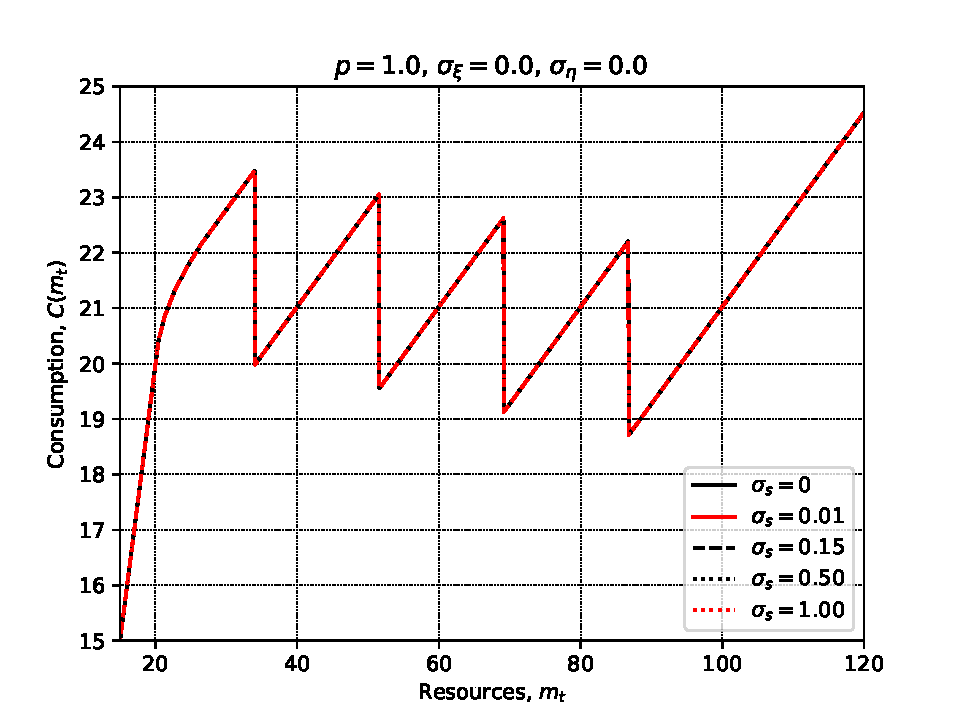
\includegraphics[width=\linewidth]{p1_xi0_eta0.pdf}
    \caption{Have switching option with certainty, $p = 1$.}
\end{subfigure}
\hfill
\begin{subfigure}{0.48\textwidth}
    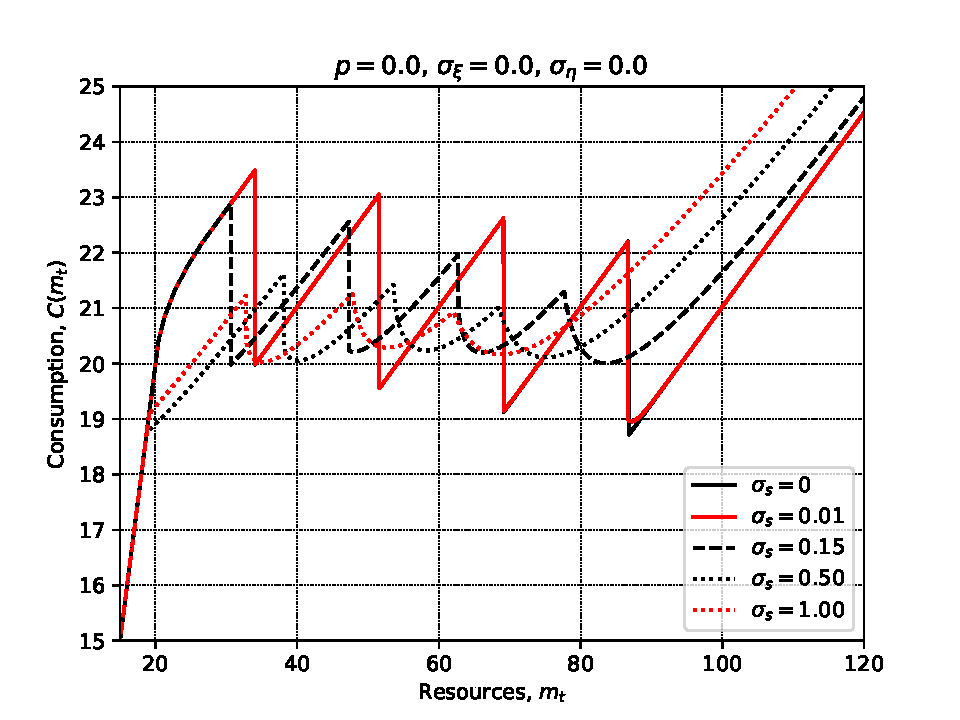
\includegraphics[width=\linewidth]{p0_xi0_eta0.pdf}
    \caption{Stay as worker with certainty without search effort, $p = 0$.}
\end{subfigure}
\caption{The plots show optimal consumption rules of the workers who decides to continue working in period
$t = T - 5$ for a set of search cost scales $\sigma_s$ in the absence of income uncertainty or taste shocks, for the
case with $p = 1.0$ (left panel) with $p = 0.0$ (right panel). The rest of the model parameters are $R = 1$,
$\beta = 0.98$, $y = 20$.}
\label{fig:fig2}
\end{figure}

In contrast, when $p = 0.0$ (Fig.~\ref{fig:fig2}(b)), the worker who does not exert search effort,
continues to stay as a worker with certainty. This gives the worker a motive to exert
search effort, which determines the likelihood of receiving the option to switch. For a
given level of search frictions, decreasing $p$ increases the smoothness of the solution.
Moreover, for a given level of $p$, increasing the search frictions (higher value of $\sigma_s$) also
increases smoothness. Fig.~\ref{fig:fig2}(b) also shows the asymmetric smoothness offered by search,
when there are no taste or income shocks. The smoothness happens to the right of the
discontinuities. This is because for low liquid resources, workers optimally choose to
continue working and hence do not exert any search effort. Workers only exert positive
effort to receive the option to retire when they have ample liquid resources. Therefore,
the smoothness from search frictions only happens to the right of the discontinuities.

To address this asymmetric smoothness, we need to introduce taste shocks. Since
the taste shocks can take a range of different values, there are certain realizations of
the taste shock that make the worker want to have the option to switch, even at levels
of liquid assets at which, in the absence of a taste shock, the worker would not want
to switch. In other words, with the introduction of taste shocks, the range of liquid
assets around the discontinuities over which the worker exerts search effort expands.
Fig.~\ref{fig:fig3}(a) shows that with the incorporation of taste shocks, the consumption function now
smoothes out more uniformly around the discontinuities. Moreover, introducing taste
shocks allows the search frictions to significantly smooths out most of the discontinuities
in the optimal consumption function. This holds even for a very small smoothness
parameter for the taste shocks, $\sigma_\xi = 0.005$. This is because now there is a positive
likelihood of a worker receiving a taste shock that makes them exert search effort even
for values of $M_t$ for which the worker would not exert any search effort in the absence
of taste shocks. Increasing the magnitude of the taste shocks to $\sigma_\xi = 0.02$ (Fig.~\ref{fig:fig3}(b))
significantly reduces the size of all the discontinuities in the consumption function.
Moreover, only moderately sized search frictions are needed to virtually completely
smooth out the consumption function.

%---- Figure 3 ----
\begin{figure}[htbp]
\centering
\begin{subfigure}{0.48\textwidth}
    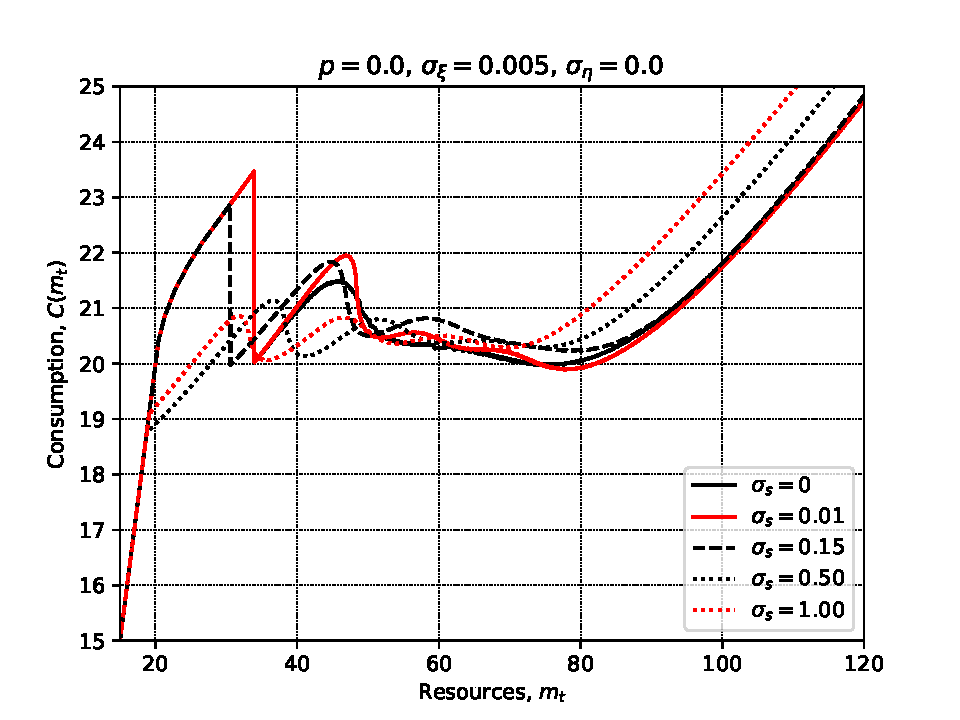
\includegraphics[width=\linewidth]{p0_xi0p005_eta0.pdf}
    \caption{Small taste shocks, $\sigma_\xi = 0.005$.}
\end{subfigure}
\hfill
\begin{subfigure}{0.48\textwidth}
    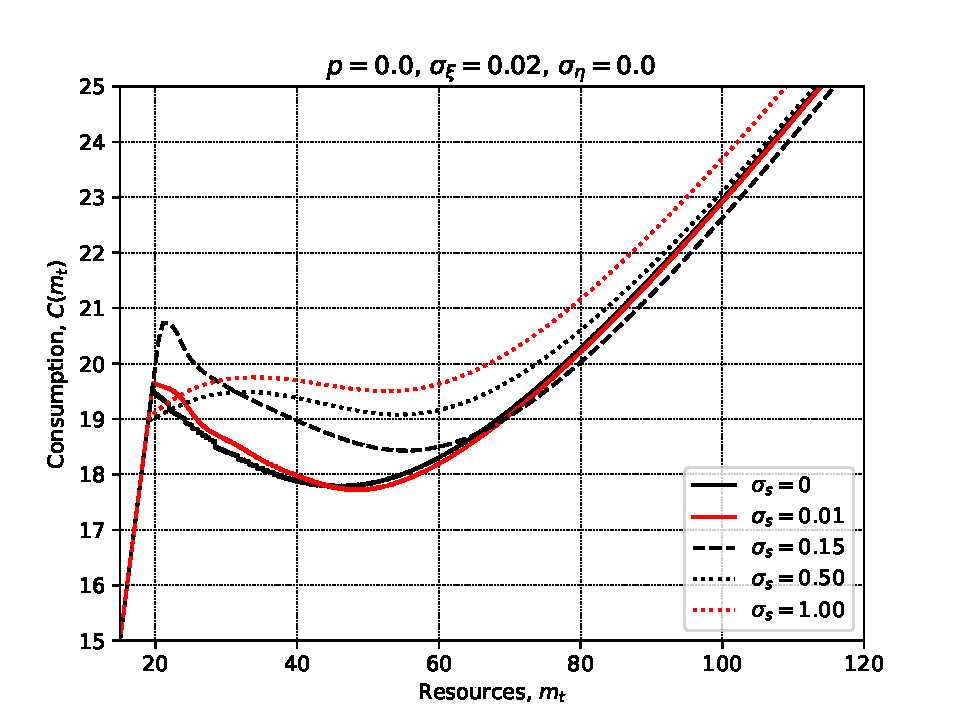
\includegraphics[width=\linewidth]{p0_xi0p02_eta0.pdf}
    \caption{Large taste shocks, $\sigma_\xi = 0.02$.}
\end{subfigure}
\caption{The plots show optimal consumption rules of the workers who decides to continue working in period
$t = T - 5$ for the case with $p = 0$, in the presence of small taste shocks (left panel) and large taste shocks
(right panel), without income uncertainty.}
\label{fig:fig3}
\end{figure}

The results discussed so far do not include any income uncertainty. Adding
income uncertainty even into standard consumption-saving models adds curvature and
smoothness to the consumption rules. We study the impact of incorporating income
uncertainty to the retirement problem on the smoothness of the decision rules in
Figs.~\ref{fig:fig4}(a) and~\ref{fig:fig4}(b). These figures show that while income uncertainty adds smoothness, it does
not play a significant role in reducing the size of the discontinuities. Therefore, search
frictions and taste shocks play the dominant role in smoothing out the problem. An
appropriate combination of search frictions, taste shocks, and income uncertainty can
yield a monotonically increasing outcome-specific consumption function by smoothing
out the discontinuities that propagate through each period while iterating backwards.

%---- Figure 4 ----
\begin{figure}[htbp]
\centering
\begin{subfigure}{0.48\textwidth}
    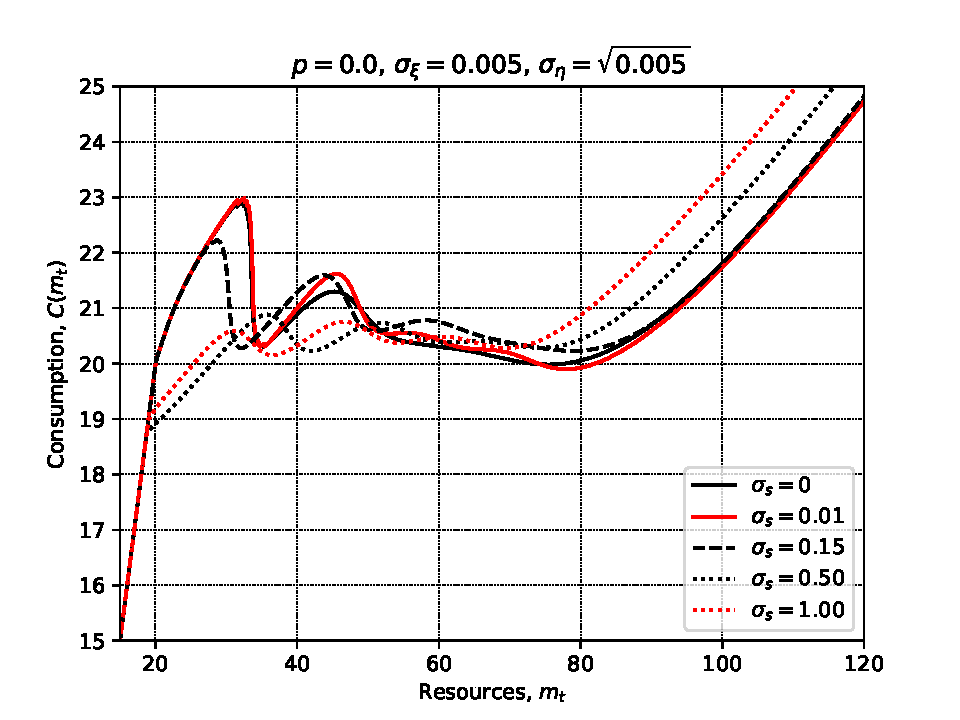
\includegraphics[width=\linewidth]{p0_xi0p005_etaSqrt0p005.pdf}
    \caption{Small taste shocks, $\sigma_\xi = 0.005$.}
\end{subfigure}
\hfill
\begin{subfigure}{0.48\textwidth}
    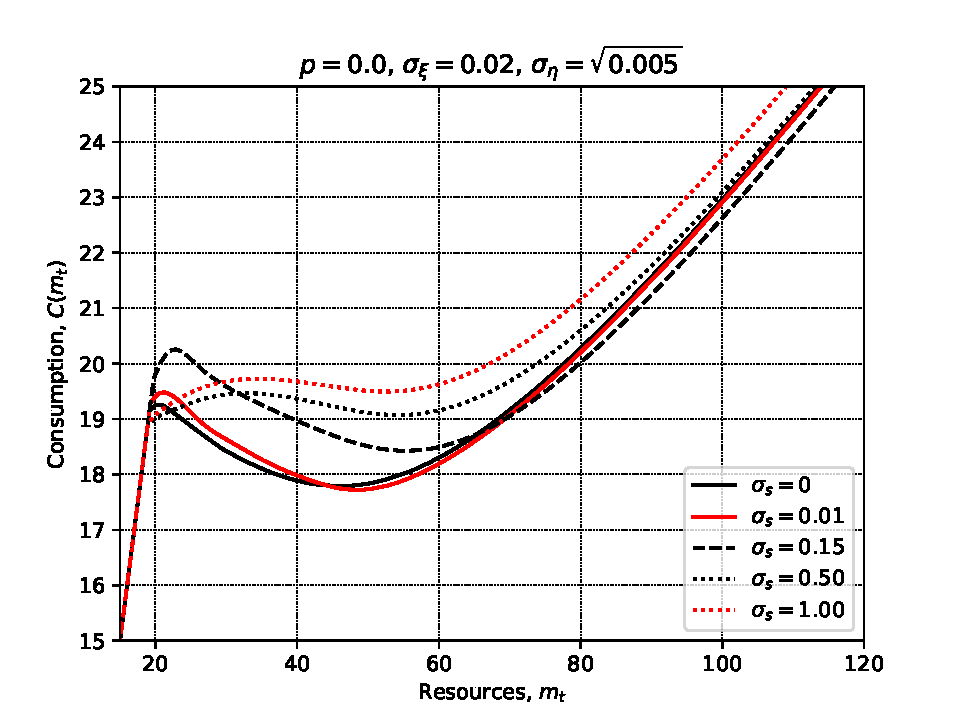
\includegraphics[width=\linewidth]{p0_xi0p02_etaSqrt0p005.pdf}
    \caption{Large taste shocks, $\sigma_\xi = 0.02$.}
\end{subfigure}
\caption{The plots show optimal consumption rules of the workers who decides to continue working in period
$t = T - 5$ for the case with $p = 0$, in the presence of small taste shocks (left panel) and large taste shocks
(right panel), with income uncertainty.}
\label{fig:fig4}
\end{figure}

It is important to note that although each of these smoothness mechanisms serve
to smooth out the solution for the worker's problem, they have different economic
interpretations and affect the optimal consumption rule differently. While lowering
the exogenous probability of receiving the option to switch, $p$, and increasing the search
frictions, $\sigma_s$, shift the consumption function upwards, large taste shocks, $\sigma_\xi$, and income
shocks, $\sigma_\eta$, shift the consumption function downwards. Ceteris paribus, decreasing
$p$ or increasing $\sigma_s$, reduce the likelihood of the worker switching their discrete state
successfully. This means that the likelihood of the worker retiring in a given period
decreases. As a result, the expected number of years that an agent works increases
and they save less in a given period. In contrast, when the size of the taste shocks is
increased, the uncertainty surrounding the likelihood of a worker's retirement decision
increases. Consequently, the agents save more in a given period, because unexpectedly
retiring early would limit the resources that the agent can consume for the remainder of
their life. Similarly, when the size of the income shocks increases, households increase
their buffer stock savings, and the consumption function shifts down. Therefore,
although each of the smoothness mechanisms achieve the common goal of `concavifying'
the solution, they have different interpretations and different impacts on the optimal
consumption rule.

To illustrate these points graphically, we start from the baseline consumption function
that has the discontinuities completely smoothed out using smoothness parameters $p =
0$, $\sigma_\xi = 0.02$, $\sigma_s = 0.5$, and $\sigma_\eta = \sqrt{0.005}$. Fig.~\ref{fig:fig5}(a) shows the impact of lowering $p$ from the
baseline level to $p = 0.1$ and $p = 0.5$, which decreases smoothness, and Fig.~\ref{fig:fig5}(b) shows the
impact of increasing the search frictions from the baseline level to $\sigma_s = 1.0$ and $\sigma_s = 2.0$,
which increases smoothness. As mentioned above, increasing smoothness by adjusting
either of the two mechanisms shifts the optimal consumption rule upwards. On the
other hand, Fig.~\ref{fig:fig6}(a) shows the impact of increasing the size of the taste shocks from the
baseline level to $\sigma_\xi = 0.025$ and $\sigma_\xi = 0.03$, and Fig.~\ref{fig:fig6}(b) shows the impact of increasing the
size of the income shocks from the baseline level to $\sigma_\eta = 5\sqrt{0.005}$ and $\sigma_\eta = 7.5\sqrt{0.005}$.
These figures demonstrate that, as expected, increasing the magnitude of the taste or
income shocks shifts the optimal consumption function downwards. Therefore, while a
combination of these smoothing mechanisms will smooth out the discontinuities, it is
also important to note how each of them shift the decision rule differently.

%---- Figure 5 ----
\begin{figure}[htbp]
\centering
\begin{subfigure}{0.48\textwidth}
    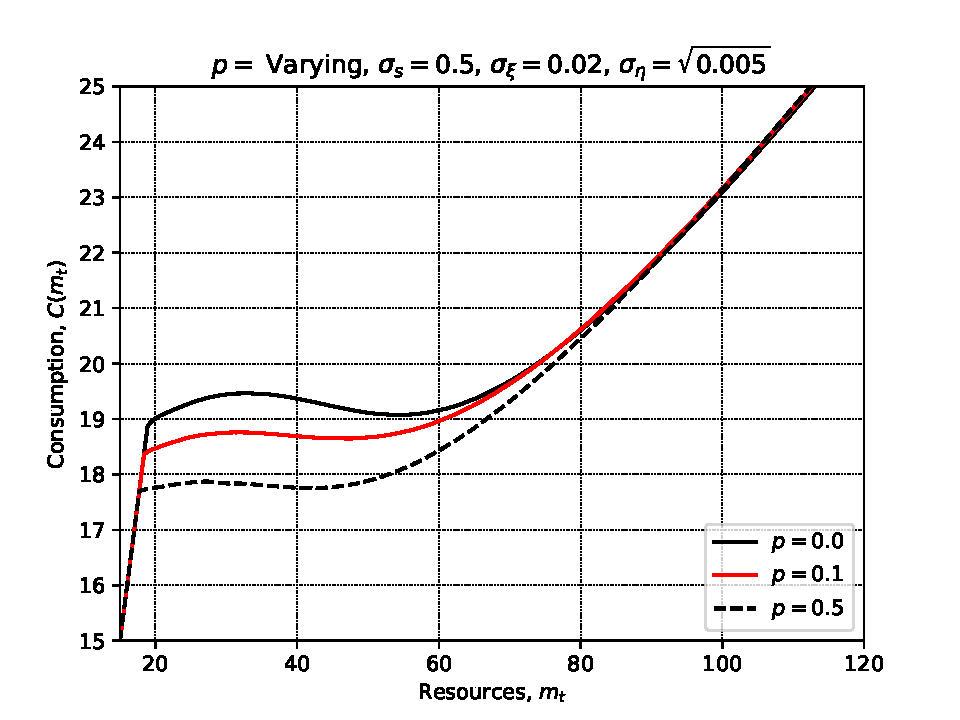
\includegraphics[width=\linewidth]{VaryP.pdf}
    \caption{Varying the exogenous probability of receiving the option to switch.}
\end{subfigure}
\hfill
\begin{subfigure}{0.48\textwidth}
    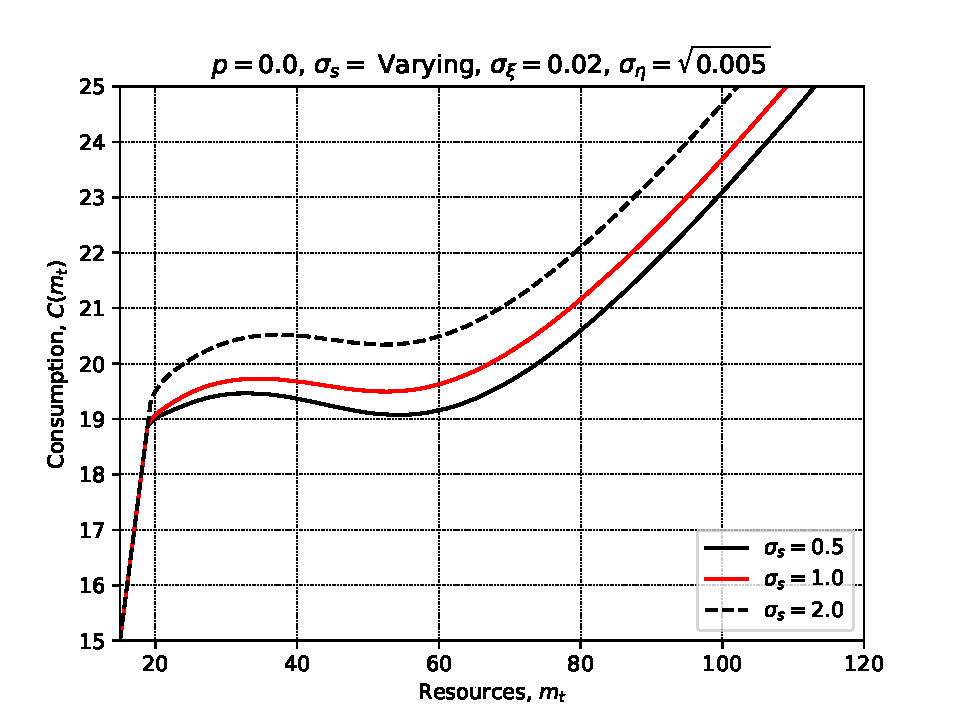
\includegraphics[width=\linewidth]{VaryS.pdf}
    \caption{Varying search friction intensity.}
\end{subfigure}
\caption{The plots show the impact of increasing the smoothness parameters for the exogenous option probability
(left panel) and increasing the magnitude of the search frictions (right panel).}
\label{fig:fig5}
\end{figure}

%---- Figure 6 ----
\begin{figure}[htbp]
\centering
\begin{subfigure}{0.48\textwidth}
    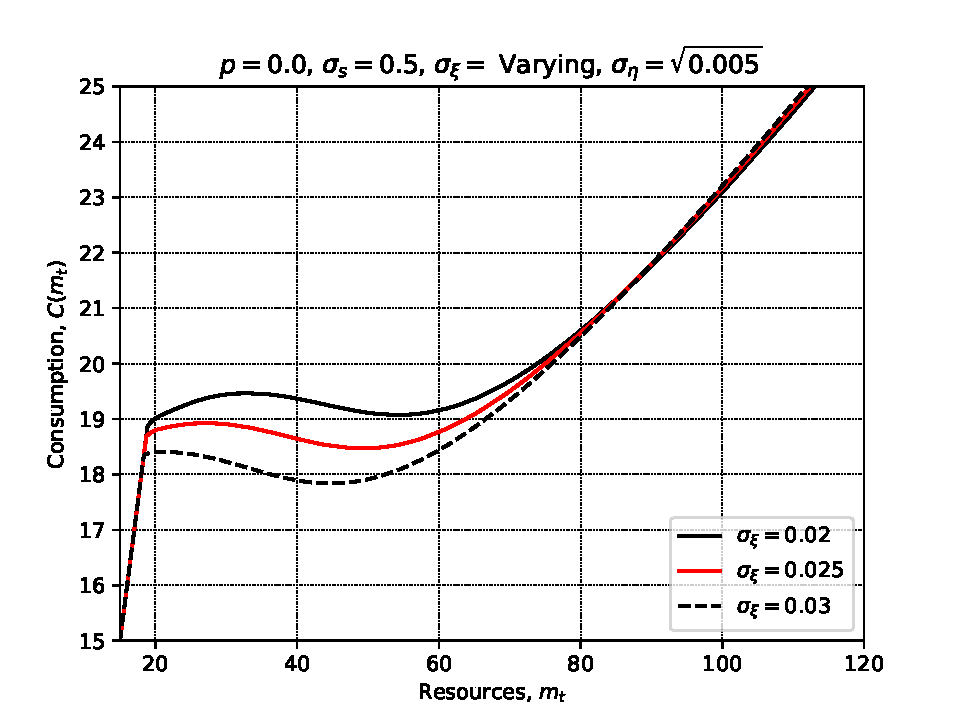
\includegraphics[width=\linewidth]{VaryXi.pdf}
    \caption{Varying the magnitude of the taste shocks.}
\end{subfigure}
\hfill
\begin{subfigure}{0.48\textwidth}
    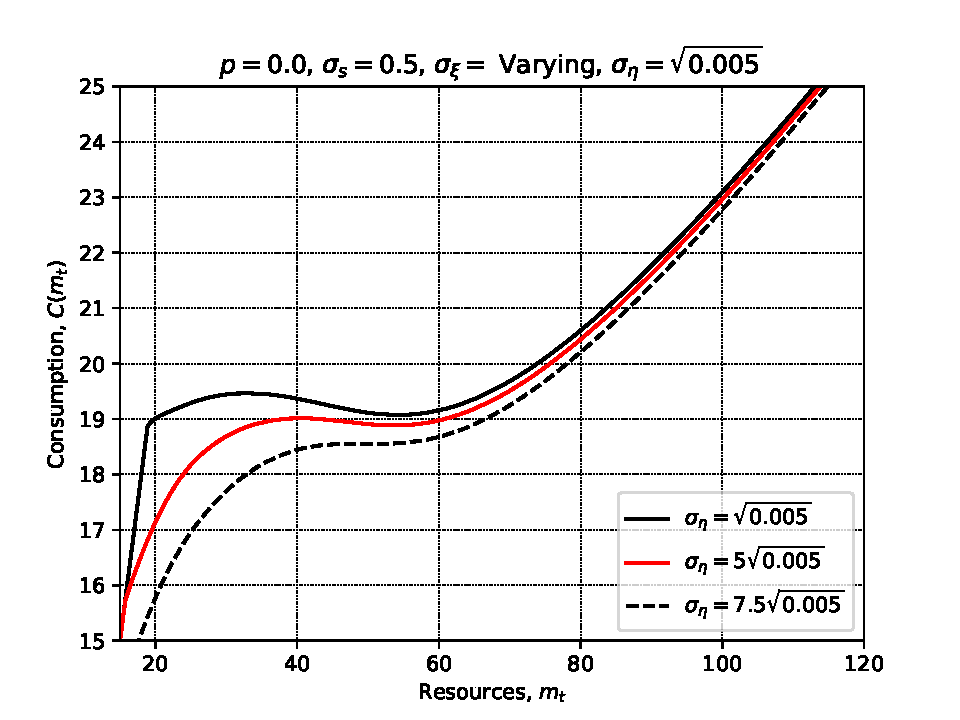
\includegraphics[width=\linewidth]{VaryEta.pdf}
    \caption{Varying the magnitude of the income shocks.}
\end{subfigure}
\caption{The plots show the impact of increasing the smoothness parameters for the taste shocks (left panel) and
increasing the magnitude of the income shocks (right panel).}
\label{fig:fig6}
\end{figure}

%============================================================
\subsection{Income discretization and phantom kinks}
\label{sec:incdisc}
%============================================================

The smoothing mechanisms studied above are \emph{economic}: they reshape the agent's
decision rule. This subsection instead isolates a \emph{numerical} source of
non-smoothness that must not be confused with the economic discontinuities from discrete
retirement. When the continuous transitory income density is replaced by a coarse
equiprobable grid, the expectation over next-period marginal utility is a sum over a few
nodes. That discrete approximation injects \emph{phantom kinks} into the outcome-specific
consumption function---spurious non-monotonicities that have no counterpart in the
underlying continuous-income problem. The economic kinks associated with the retirement
option remain part of the true solution; the phantom kinks should not.

\paragraph{Experiment.}
To isolate income integration, we shut down other smoothing channels: $p = 1$
(so $\sigma_s = 0$) and no taste shocks ($\sigma_\xi = 0$, one taste node). We set
$\sigma_\eta = \sqrt{0.005}$, matching the paper's income-shock figures, and compare:
\begin{enumerate}
    \item \emph{Discretization} of the mean-one lognormal transitory shock with
    $N \in \{1,7,31,151\}$ equiprobable nodes;
    \item the \emph{transition-matrix} method (Section~\ref{sec:tranmatrix}), which
    integrates the same continuous density via a precomputed $b\to m$ matrix
    ($500\times 510$ income grids here).
\end{enumerate}
Other parameters are $R = 1$, $\beta = 0.98$, $y = 20$. Figure~\ref{fig:incdisc} plots
the working-state consumption rule over $m \in [15,120]$.

\begin{figure}[htbp]
\centering
    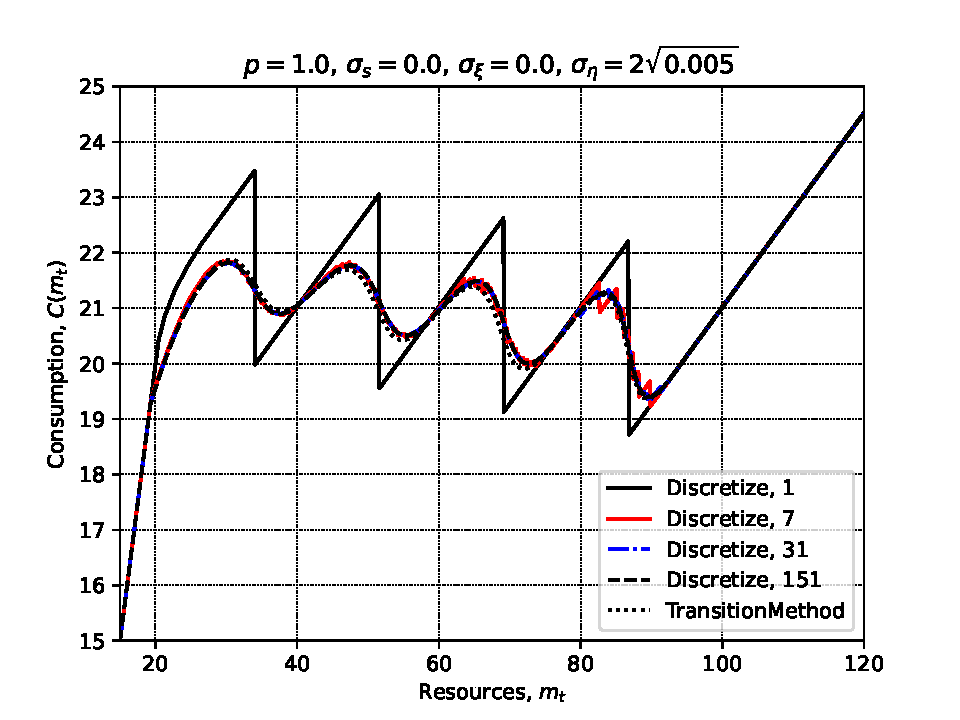
\includegraphics[width=0.6\linewidth]{IncomeDiscMethod_Convergence.pdf}
\caption{Phantom kinks from income discretization. Coarse $N$ produces spurious
wiggles in $C(m)$; refining $N$ (or using the transition matrix) removes them.
Held fixed: $\sigma_\eta = \sqrt{0.005}$, $p = 1$, $\sigma_s = 0$, $\sigma_\xi = 0$.
The remaining curvature is the economically relevant discrete-choice pattern, not a
discretization artifact.}
\label{fig:incdisc}
\end{figure}

\paragraph{What the figure shows.}
With $N=1$ the consumption rule exhibits large sawtooth phantom kinks. Raising $N$ to
$7$ and then $31$ damps those artifacts; at $N=151$ they are essentially gone and the
rule is smooth aside from the economic discrete-choice structure. The transition-matrix
solution overlays that fine-discretization \emph{smoothness}: it does not reintroduce
the coarse-$N$ zigzags. That is the sense in which the method ``works''---it targets
the continuous income integral that the discrete nodes only approximate.

\paragraph{Benchmarking caveat.}
A natural quantitative check is the pointwise gap between each method and the
$N=151$ discretization. We report solve times and that gap in Table~\ref{tab:incdisc},
but with an important caveat: $N=151$ is still a \emph{discrete} income approximation,
not the continuous-income truth. Small residual differences between the transition
matrix and $N=151$ therefore need not mean the matrix is ``wrong''; they can reflect
two different approximations to the same continuous expectation. Moreover, those gaps
are \emph{horizon-dependent}: near the terminal period the two methods are very close,
while earlier periods accumulate integration differences, so a max-absolute deviation
versus $N=151$ can grow even when neither rule displays phantom kinks. The right visual
benchmark for the paper's claim is therefore Figure~\ref{fig:incdisc} (presence or
absence of spurious non-monotonicities), not a claim that the matrix is uniformly
closer to $N=151$ than every coarser $N$ at every $t$.

\begin{table}[htbp]
\centering
\caption{Solve time by income-integration method
($\sigma_\eta = \sqrt{0.005}$, $p=1$, $\sigma_s=0$, $\sigma_\xi=0$).
Max.\ / mean abs.\ deviation of $C(m)$ vs.\ $N=151$ on $m\in[15,120]$ are reported
as a diagnostic only (see text); they are not the success criterion for removing
phantom kinks.}
\label{tab:incdisc}
\begin{tabular}{lcccc}
\toprule
Method & Gridpoints & Solve time (s) & Max.\ abs.\ vs $151$ & Mean abs.\ vs $151$ \\
\midrule
Discretization    & $1$   & $0.50$ & $4.72$ & $0.023$ \\
Discretization    & $7$   & $0.66$ & $4.68$ & $0.004$ \\
Discretization    & $31$  & $1.60$ & $0.094$ & $0.001$ \\
Discretization    & $151$ & $14.3$ & $0$ & $0$ \\
Transition matrix & ---   & $4.10$ & $0.034$ & $0.0005$ \\
\bottomrule
\end{tabular}
\end{table}

\noindent
Table~\ref{tab:incdisc} also makes the cost point: obtaining a kink-free rule by pushing
discretization to $N=151$ is expensive relative to a moderate transition-matrix grid that
achieves the same qualitative smoothness in Figure~\ref{fig:incdisc}.

\paragraph{Note on shock size.}
The illustration uses $\sigma_\eta = \sqrt{0.005}$, as in the paper's other income-shock
figures. The transition matrix employs a fixed $(b,m)$ support; if $\sigma_\eta$ is
scaled up substantially (e.g.\ $2\sqrt{0.005}$), more mass sits near the grid edge and
the same matrix can diverge more from a fine discretization unless the income grids are
widened and refined (at cost scaling with the product of the grid sizes). The phantom-kink
lesson---coarse $N$ creates numerical wiggles; continuous integration or fine $N$ removes
them---is not tied to that particular $\sigma_\eta$, but quantitative gaps versus a
fixed $N=151$ benchmark are.

%============================================================
\subsection{Algorithm}
%------------------------------------------------------------
This section outlines the algorithm for solving the problem of the worker who continues
to work in the current period. The problem for the retiree can be pre-solved relatively
easily. With the solution of the worker who continues to work and the retiree at hand,
it is straightforward to compute the solution of the worker with the option to switch.
With ample smoothness, the EGM-step should not produce any suboptimal points.
However, if there is not enough smoothness, then an additional `upper envelope' step
is required to remove the suboptimal points. The upper envelope refinement step in
\citet{Iskhakov2017-jb} is an example of an algorithm that
can be employed at the end of the EGM-step to achieve this.

\begin{algorithm}[htbp]
\caption{EGM-step with search for the worker who continues to work}
\DontPrintSemicolon
Let $\vec{\eta} = \{\eta_1, \dots, \eta_J\}$ and $\vec{\xi} = \{\xi_1, \dots, \xi_K\}$ be vectors of quadrature points with associated weights
$\vec{\omega} = \{\omega_1, \dots, \omega_J\}$ and $\vec{\mu} = \{\mu_1, \dots, \mu_K\}$, respectively.\;
Form an ascending grid over end-of-period wealth, $\vec{A}_t = \{A_t^1, \dots, A_t^I\}$\;
\For{$i = 1, \dots, I$}{
    \For{$j = 1, \dots, J$}{
        Compute $M_{t+1}^j(A_i) = R A_i + y \eta_{t+1}^j$\;
        \For{$d_{t+1} = 0, 1$}{
            Compute $c_{t+1}^{\Ret}(M_{t+1}^j(A_i))$ by interpolating $c_{t+1}^{\Ret}(\vec{M}_{t+1})$ at the point $M_{t+1}^j(A_i)$\;
            Compute $c_{t+1}^{W}(M_{t+1}^j(A_i))$ by interpolating $c_{t+1}^{W}(\vec{M}_{t+1})$ at the point $M_{t+1}^j(A_i)$\;
            Compute $V_{t+1}^{\Ret}(M_{t+1}^j(A_i))$ by interpolating $V_{t+1}^{\Ret}(\vec{M}_{t+1})$ at the point $M_{t+1}^j(A_i)$\;
            \For{$k = 1, \dots, K$}{
                Compute $V_{t+1}^{W}(M_{t+1}^j(A_i), \xi_k)$ by interpolating $V_{t+1}^{W}(\vec{M}_{t+1})$ at the point $M_{t+1}^j(A_i)$ and multiplying it by $\xi_k$\;
                Compute $V_{t+1}^{RW}(M_{t+1}^j(A_i), \xi_k) = \max\{V_{t+1}^{\Ret}(M_{t+1}^j(A_i)), V_{t+1}^{W}(M_{t+1}^j(A_i), \xi_k)\}$\;
                Compute $\mathbbm{1}_{t+1}^0(M_{t+1}^j(A_i), \xi_k) = 1$ if $V_{t+1}^{\Ret}(M_{t+1}^j(A_i)) \ge V_{t+1}^{W}(M_{t+1}^j(A_i), \xi_k)$ and $0$ otherwise.\;
                Compute $\mathbbm{1}_{t+1}^1(M_{t+1}^j(A_i), \xi_k) = 1 - \mathbbm{1}_{t+1}^0(M_{t+1}^j(A_i), \xi_k)$\;
                Compute $\mathrm{RHS}_1^{\mathrm{pre}}(M_{t+1}^j(A_i), \xi_k) = \mathbbm{1}_{t+1}^0(M_{t+1}^j(A_i), \xi_k) \cdot u'(c_{t+1}^{\Ret}(M_{t+1}^j(A_i))) + \xi_k \cdot \mathbbm{1}_{t+1}^1(M_{t+1}^j(A_i), \xi_k) \cdot u'(c_{t+1}^{W}(M_{t+1}^j(A_i)))$\;
                Compute $\mathrm{RHS}_2^{\mathrm{pre}}(M_{t+1}^j(A_i), \xi_k) = \xi_k \cdot u'(c_{t+1}^{W}(M_{t+1}^j(A_i)))$\;
            }
        }
    }
    Compute $\goth{V}_t^1(A_i) = \sum_{j=1}^{J} \sum_{k=1}^{K} \omega_j \mu_k \cdot V_{t+1}^{RW}(M_{t+1}^j(A_i), \xi_k)$\;
    Compute $\goth{V}_t^2(A_i) = \sum_{j=1}^{J} \sum_{k=1}^{K} \omega_j \mu_k \cdot V_{t+1}^{W}(M_{t+1}^j(A_i), \xi_k)$\;
    Compute $\eff_t(A_i) = 1 - \exp\left(-\beta(1 - p)(\goth{V}_t^1(A_i) - \goth{V}_t^2(A_i))/\sigma_s\right)$\;
    Compute $\theta(\eff_t(A_i)) = \sigma_s (\eff_t(A_i) + (1 - \eff_t(A_i)) \log(1 - \eff_t(A_i)))$\;
    Compute $P_1(\eff_t(A_i)) = (1 - \eff_t(A_i)) \cdot p + \eff_t(A_i)$\;
    Compute $P_2(\eff_t(A_i)) = (1 - \eff_t(A_i)) \cdot (1 - p)$\;
    Compute $\mathrm{RHS}_1(A_i) = \sum_{j=1}^{J} \sum_{k=1}^{K} \omega_j \mu_k \cdot \mathrm{RHS}_1^{\mathrm{pre}}(M_{t+1}^j(A_i), \xi_k)$\;
    Compute $\mathrm{RHS}_2(A_i) = \sum_{j=1}^{J} \sum_{k=1}^{K} \omega_j \mu_k \cdot \mathrm{RHS}_2^{\mathrm{pre}}(M_{t+1}^j(A_i), \xi_k)$\;
    Compute $\mathrm{RHS}(A_i) = R\beta (P_1(\eff_t(A_i)) \mathrm{RHS}_1(A_i) + P_2(\eff_t(A_i)) \mathrm{RHS}_2(A_i))$\;
    Compute expected value function $\E V_{t+1}(M_{t+1}(A_i)) = P_1(\eff_t(A_i)) \cdot \goth{V}_t^1(A_i) + P_2(\eff_t(A_i)) \cdot \goth{V}_t^2(A_i)$\;
    Compute current consumption $c_t^{W}(A_i) = u'^{-1}(\mathrm{RHS}(A_i))$\;
    Compute value function $V_t^{W}(M_t(A_i)) = u(c_t^{W}(A_i), 1, \eff_t(A_i)) + \beta \E V_{t+1}(M_{t+1}(A_i))$\;
    Compute endogenous grid point $M_t(A_i) = c_t^{W}(A_i) + A_i$\;
}
Collect the points $M_t(A_i)$, $c_t^{W}(A_i)$, and $V_t^{W}(M_t(A_i))$ to form the consumption function, $c_t^{W}(\vec{M}_t)$, and value function, $V_t^{W}(\vec{M}_t)$.\;
\end{algorithm}

%------------------------------------------------------------
\subsubsection{Transition-matrix income integration}
\label{sec:tranmatrix}
%------------------------------------------------------------

In Algorithm~1, the expectation over the transitory income shock is taken by looping over
the $J$ quadrature nodes $\vec{\eta}$ and interpolating the next-period functions at each
implied $M_{t+1}^j(A_i)$. As an alternative, the transitory-income integration can be
recast as a single (precomputed) linear map, following the transition-matrix approach of
\citet{White2015-fz}.

\paragraph{Idea.}
Let $b = R A_t$ denote next-period wealth \emph{before} the income draw, and
$m = R A_t + y\eta$ next-period market resources \emph{after} it. For a fixed income
process, the conditional density of $m$ given $b$ is time-invariant, so the mapping from a
function defined on an $m$-grid to its conditional expectation on a $b$-grid can be encoded
once as a matrix $\Pi$ with entries $\Pi_{b,m} \approx \Pr(m \mid b)$.

\paragraph{Steps.}
\begin{enumerate}
    \item Build dense grids over $b$ and $m$ (exponentially spaced) and construct $\Pi$
    from the mean-one lognormal transitory density. Because the $m$-grid is non-uniform,
    each density evaluation is weighted by the local grid spacing $\Delta m$ before
    row-normalization (so that $\Pi$ approximates $\int f(m)\,g(m-b)\,dm$ rather than an
    equally weighted sum over columns). Probability mass mapped outside the tabulated
    $m$-range is dropped and each row is renormalized to sum to one.
    \item For each next-period quantity of interest (marginal utility and value), evaluate
    it on the $m$-grid, then obtain its conditional expectation on the $b$-grid by the
    matrix product $\Pi \, f(\vec{m})$. Expectations are then interpolated onto
    $b = R\,\vec{A}_t$ in inverse form (CRRA-inverse for marginal utilities;
    $V_T = -1/V$ for values) before the EGM step.
    \item The remaining EGM and envelope steps of Algorithm~1 are unchanged.
\end{enumerate}

\paragraph{Rationale.}
Because $\Pi$ is assembled once and reused across periods, the per-period cost of the
income expectation reduces to a matrix multiplication. Relative to a coarse
equiprobable shock grid, the matrix integrates the continuous density and thereby
avoids the phantom kinks documented in Section~\ref{sec:incdisc}
(Figure~\ref{fig:incdisc}), typically at lower cost than pushing discretization to a
very fine $N$ (Table~\ref{tab:incdisc}). As noted there, a fixed $(b,m)$ grid may need
widening if $\sigma_\eta$ is scaled up substantially.

%============================================================
\section{Retirement model with stochastic account realizations}\label{sec:RetirementModelPrices}
%============================================================
The retirement application of Section~\ref{sec:RetirementModel} smooths the work--retire margin with three mechanisms: an exogenous probability $p$ of receiving the option to switch, directed search at convex cost, and multiplicative log-normal taste shocks, with transitory income risk as a fourth, continuous-choice, smoother. This section introduces idiosyncratic price dispersion as a fifth source of variatition.

The idea is very intuitively discribed in Section~\ref{sec:DurableModel} for a durable goods model. In the durable model the household searches for a car; contingent on a successful search it observes a stochastic price $p_t$ and then decides whether to buy or to keep. Here the household searches for the option to retire; contingent on receiving that option it observes a stochastic realization of its retirement account and then decides whether to take the draw---retire, absorbing, with that wealth---or to deny it and work another period. Continuing to work is the analog of keeping; claiming the realized account is the analog of adjusting at the realized price. Because $p$ already denotes the exogenous option probability, we write $\phi_t$ for the account realization. Agents who have the option observe $\phi_t$ before choosing and can reject an unattractive draw by remaining at work. Detailed derivations---envelope conditions, Euler equations, the interaction with search, and the EGM algorithm---are in Appendix~\ref{sec:appdx_retirement}.

%------------------------------------------------------------
\subsection{Extension: Stochastic retirement wealth}\label{subsec:RetirementPrices}
%------------------------------------------------------------
This subsection isolates account-value dispersion from the other retirement smoothers, in the same spirit as Section~\ref{subsec:ModelBasicPrice}. Neither taste shocks nor search frictions are present, so a worker who receives the option to retire resolves the discrete choice by a hard maximum. The comparison itself is contingent on the realized account value; the retiree's \emph{problem}, once the draw has been accepted, is not. To shut down search we set the exogenous option probability to $p=1$, so the option---and therefore a draw of $\phi_t$---arrives with certainty and optimal effort is identically zero.

At the start of period $t$, after the transitory income shock $\eta_t$ has materialized and beginning-of-period book resources $M_t$ are known, the household observes an i.i.d.\ multiplicative realization of the retirement account
\begin{align}
	\log \phi_t \sim \mathcal{N}\Big(-\frac{\sigma_\phi^2}{2},\,\sigma_\phi^2\Big),
	\qquad \mathbb{E}[\phi_t]=1, \label{eq:ret_price_dist}
\end{align}
independent of $\eta_t$ and independent across periods. If the household claims, retirement begins with wealth
\begin{align}
	\tilde M_t = \phi_t M_t, \label{eq:ret_price_Mtilde}
\end{align}
and from that point the agent is an ordinary retiree: the Bellman problem, budget $A_t=\tilde M_t-c_t$, and Euler equation are exactly those of Section~\ref{sec:RetirementModel}, evaluated at $\tilde M_t$ rather than at $M_t$. If the household denies the draw, it remains a worker with book resources $M_t$ and the standard budget $A_t=M_t-c_t$; the realization $\phi_t$ is discarded. The draw is therefore a one-shot, rejectable mark-to-market of the nest egg at the moment of claiming---a stochastic liquidation value, annuity conversion factor, or defined-contribution account realization---not an ongoing price of consumption in retirement. Once the draw is accepted, $\phi_t$ is locked into the level of wealth and is not redrawn.

This is the analog of the durable model's assumption that only the \emph{purchase} of new durables is exposed to $p_t$. The worker who does not claim never transacts in the retirement account, just as the keeper never transacts in the durable market. A high realization of $\phi_t$ raises the value of retiring and, conditional on claiming, the resources out of which the retiree consumes; a low realization has the opposite effect and can be rejected.

The retiree's problem is therefore unchanged in form. Write $V_t^{\Ret}(\cdot)$ for the baseline retiree value of Section~\ref{sec:RetirementModel}. The value of claiming at the realized account is simply that function evaluated at scaled wealth,
\begin{align}
	V_t^{\Ret}(\tilde M_t)
	= V_t^{\Ret}(\phi_t M_t),
	\label{eq:ret_price_VRet}
\end{align}
with claiming-period consumption $c_t^{\Ret}(\phi_t M_t)$ read off the same baseline policy. There is no separate price-contingent retiree Euler equation and no need to re-solve the retiree problem at each quadrature node of $\phi$: unlike the durable adjuster, whose first-order condition in $d_t$ depends on $p_t$ (equation~\eqref{eq:price_foc_d}), the intensive margin here is movement along a single consumption function.

The worker who does not claim solves, with $p=1$ and no taste shocks,
\begin{align}
	V_t^{W}(M_t)
	&= \max_{0\le c_t\le M_t}
	\left\{
		\log(c_t)-\delta
		+ \beta\,\goth{V}_t^{1}(A_t)
	\right\},
	\label{eq:ret_price_VW}
\end{align}
with $A_t=M_t-c_t$ and $\goth{V}_t^{1}$ the expected value of saving $A_t$ when the option---and a fresh draw of $\phi$---arrives next period.

Because $\phi_t$ is observed before the discrete choice is made, the beginning-of-period problem of a worker who has the option is the realization-contingent hard maximum
\begin{align}
	V_t(M_t,\phi_t)
	= \max\Big\{
		V_t^{\Ret}(\phi_t M_t),\;
		V_t^{W}(M_t)
	\Big\}.
	\label{eq:ret_price_discrete}
\end{align}
A high $\phi_t$ makes claiming more attractive and, if accepted, delivers higher retirement consumption along $c_t^{\Ret}(\cdot)$; a low $\phi_t$ makes claiming less attractive and is denied whenever $V_t^{\Ret}(\phi_t M_t)<V_t^{W}(M_t)$. The model therefore induces state-contingent variation in both the retirement margin and the wealth at which the retiree starts, while leaving the retiree's decision \emph{rule} unchanged.

As with the price-integrated durable value~\eqref{eq:price_barv}, the object that matters for the previous period's continuation is
\begin{align}
	\bar V_t(M_t)
	\equiv \mathbb{E}_{\phi_t}\big[V_t(M_t,\phi_t)\big]
	= \mathbb{E}_{\phi_t}\Big[
		\max\big\{
			V_t^{\Ret}(\phi_t M_t),\;
			V_t^{W}(M_t)
		\big\}
	\Big],
	\label{eq:ret_price_barV}
\end{align}
which replaces $V_t(M_t,\{R,W\})$ inside $\goth{V}_{t-1}^{1}$. Unlike the multiplicative taste shock $\xi_t$ of Section~\ref{sec:RetirementModel}, which scales the worker's value and thereby reweights the discrete comparison without changing either branch's consumption, $\phi_t$ changes the \emph{argument} of the retiree's consumption function. The policy $c_t^{\Ret}(\phi_t M_t)$ is realization-contingent even though the function $c_t^{\Ret}(\cdot)$ itself is not, and the model's reported (ex-ante) consumption function is the $\phi$-weighted average of the realized hard choices. As $\sigma_\phi\to 0$, $\phi_t\to 1$ almost surely and the model collapses to the hard-maximum baseline of Section~\ref{sec:RetirementModel} with $p=1$ and $\sigma_\xi=0$.

Two differences from the durable-price extension are worth flagging. First, retirement is self-absorbing, so a household that accepts $\phi_t$ cannot return to work next period to wait for a better draw; the analog of ``keeping'' is available only before claiming. Second, because $\phi_t$ rescales the state rather than the first-order condition, the retiree is solved once, and each $\phi$-node is only an evaluation point---cheaper than re-solving the durable adjuster at every $p_k$. The smoothing mechanism is nevertheless the same: integrating~\eqref{eq:ret_price_discrete} over $\phi_t$ replaces a single wealth threshold $M^\ast$ at which $V^{\Ret}(M^\ast)=V^{W}(M^\ast)$ with a family of thresholds $M^\ast(\phi)$, so the ex-ante claiming probability is interior and the expected marginal value that enters last period's Euler equation is smoothed. We derive the envelope conditions, the terminal-period solution, and the EGM algorithm in Appendix~\ref{subsec:appdx_ret_price}.

%------------------------------------------------------------
\subsection{Extension: Search and stochastic retirement wealth}\label{subsec:RetirementSearchPrices}
%------------------------------------------------------------
This subsection nests the directed-search technology of Section~\ref{sec:RetirementModel} with the stochastic account realizations of Section~\ref{subsec:RetirementPrices}. The protocol is now the full analog of searching for a car. The household chooses search effort; contingent on a successful search it receives the option to retire \emph{and} a draw of the retirement account; it then takes the draw or works another period. As in Section~\ref{subsec:ModelBasicFull}, taste shocks and directed search are alternative ways of smoothing the discrete margin, so the nested environment uses search rather than taste shocks. The exogenous option probability $p\in[0,1)$ is restored, so a worker who exerts no effort receives a draw with probability $p$ and a worker who exerts maximal effort receives one with certainty.

The account realization follows~\eqref{eq:ret_price_dist}, with $\phi_t\perp\eta_t$ and i.i.d.\ across periods. The within-period timeline is as follows. After $\eta_t$ has materialized and $M_t$ is known, the household learns whether the option arrived (determined by last period's effort). If it did not, the agent must work; $\phi_t$ is then irrelevant, because there is no account to claim. If it did, the agent observes $\phi_t$ and chooses the hard maximum~\eqref{eq:ret_price_discrete}: claim $\tilde M_t=\phi_t M_t$ and retire, or deny and work. Search effort $\eff_t$ is chosen at the end of a working period and shifts the probability of receiving a (new) draw next period, exactly as in Section~\ref{sec:RetirementModel}.

The retiree's problem remains the baseline problem evaluated at claimed wealth. The worker who must continue working solves
\begin{align}
	V_t^{W}(M_t)
	&= \max_{\substack{0\le c_t\le M_t\\ 0\le\eff_t\le 1}}
	\left\{
		\log(c_t)-\delta-\theta(\eff_t)
		+ \beta P_1(\eff_t)\,\goth{V}_t^{1}(A_t)
		+ \beta P_2(\eff_t)\,\goth{V}_t^{2}(A_t)
	\right\},
	\label{eq:ret_full_VW}
\end{align}
with $A_t=M_t-c_t$, $P_1(\eff_t)=(1-\eff_t)p+\eff_t$, $P_2(\eff_t)=(1-\eff_t)(1-p)$, and the same search-cost function $\theta(\eff_t)=\sigma_s\bigl(\eff_t+(1-\eff_t)\log(1-\eff_t)\bigr)$ as in Section~\ref{sec:RetirementModel}. Current $\phi_t$ does not enter~\eqref{eq:ret_full_VW}: a worker who did not claim does not cash the account this period. What changes is the continuation. The expected value of saving $A_t$ when the option arrives next period now integrates over next period's account draw as well as income,
\begin{align}
	\goth{V}_t^{1}(A_t)
	&= \int_{y_{t+1}}\int_{\phi_{t+1}}
	V_{t+1}\bigl(M_{t+1}(A_t),\{R,W\},\phi_{t+1}\bigr)\,
	dF(y_{t+1})\,dF(\phi_{t+1}),
	\label{eq:ret_full_gothV1}
\end{align}
where $M_{t+1}=A_t R+y_{t+1}$ (the agent worked this period) and
\begin{align}
	V_{t+1}\bigl(M_{t+1},\{R,W\},\phi_{t+1}\bigr)
	&= \max\Big\{
		V_{t+1}^{\Ret}(\phi_{t+1} M_{t+1}),\;
		V_{t+1}^{W}(M_{t+1})
	\Big\}.
	\label{eq:ret_full_discrete}
\end{align}
The expected value of saving $A_t$ when the option does \emph{not} arrive,
\begin{align}
	\goth{V}_t^{2}(A_t)
	&= \int_{y_{t+1}}
	V_{t+1}^{W}\bigl(M_{t+1}(A_t)\bigr)\,
	dF(y_{t+1}),
	\label{eq:ret_full_gothV2}
\end{align}
does not integrate over $\phi_{t+1}$, because a must-work agent cannot claim. Future draws still sit inside $V^{W}$ through $\goth{V}^{1}$ and $\goth{V}^{2}$ one period ahead.

Search effort is chosen only on the working branch, after consumption, and does not depend on the current draw (the current $\phi_t$ is already sunk from the point of view of next period's option). The closed-form effort rule of Section~\ref{sec:RetirementModel} therefore carries over with the new gothic values~\eqref{eq:ret_full_gothV1}--\eqref{eq:ret_full_gothV2}:
\begin{align}
	\eff_t^{\ast}(A_t)
	&= 1-\exp\left(
		-\frac{\beta(1-p)}{\sigma_s}
		\bigl(\goth{V}_t^{1}(A_t)-\goth{V}_t^{2}(A_t)\bigr)
	\right).
	\label{eq:ret_full_effort}
\end{align}
Account-value dispersion raises $\goth{V}_t^{1}$ relative to $\goth{V}_t^{2}$ because the option to retire is now also an option on $\phi_{t+1}$: the household claims when the draw is attractive and otherwise continues working. That option value increases the excess value of receiving the option, and therefore increases search effort---the two frictions are complements, exactly as a low durable price raises $\varepsilon_t^{\ast}$ in Section~\ref{subsec:ModelBasicFull}.

The object that enters today's Euler equations is the pair of gothic values already defined; equivalently, one may write the beginning-of-period $\phi$-integrated value of a worker who will have the option as
\begin{align}
	\bar V_t^{R,W}(M_t)
	\equiv \mathbb{E}_{\phi_t}\Big[
		\max\big\{
			V_t^{\Ret}(\phi_t M_t),\;
			V_t^{W}(M_t)
		\big\}
	\Big],
	\label{eq:ret_full_barVRW}
\end{align}
so that $\goth{V}_{t-1}^{1}(A_{t-1})=\mathbb{E}_{\eta_t}[\bar V_t^{R,W}(R A_{t-1}+y_t)]$. Equation~\eqref{eq:ret_full_VW} nests the standalone extensions: with $\sigma_\phi\to 0$ it collapses to the search problem of Section~\ref{sec:RetirementModel} (without taste shocks); with $\sigma_s\to\infty$ or $p=1$ (so $\eff_t^{\ast}=0$) it collapses to the realization-contingent hard maximum of Section~\ref{subsec:RetirementPrices}; and with both limits simultaneous it collapses to the hard-maximum baseline. We derive the combined envelope conditions, the worker's Euler equation, the terminal-period solution, and the EGM algorithm for the nested model in Appendix~\ref{subsec:appdx_ret_full}.

The two frictions play complementary roles. Search governs whether a draw arrives; $\phi_t$ is the content of the draw, and the hard maximum~\eqref{eq:ret_full_discrete} is the decision to take it or to work another period. Search alone cannot cherry-pick a good account realization, because effort is chosen before $\phi_{t+1}$ is observed; account dispersion alone cannot smooth the problem of a worker who did not receive the option, because that agent cannot claim at any $\phi$. Together they smooth both the arrival of the option and the terms on which it is exercised.


\subsection{Results}
Introducing price dispersion smooths the problem numerical with two features which figure~\ref{fig:fig8} illustrates. The left panel shows the consumption function for larger price dispersion. A higher price dispersion means that the agent could receive a much larger retirement wealth amount or a smaller amount. Therefore, agents who receive a low draw might want to wait another period and hope for a better draw in the future. As a result, larger price dispersion leads to a smoother consumption function. Numerically, it matters how many price points we are considering. The right panel shows that with only 5 points (red), we increase the number of discontinuities, but it is not enough to smooth the full consumption function. With a larger number of points and th assumption of a large number of agents, the combined consumption function consists of the average of many functions in which some agents accept and others do not. Note that for a large number of shock points -- eg 151 -- the smoothing does not change much compared to an even larger number --eg 351.


%---- Figure 8 ----
\begin{figure}[htbp]
	\centering
	\begin{subfigure}{0.48\textwidth}
		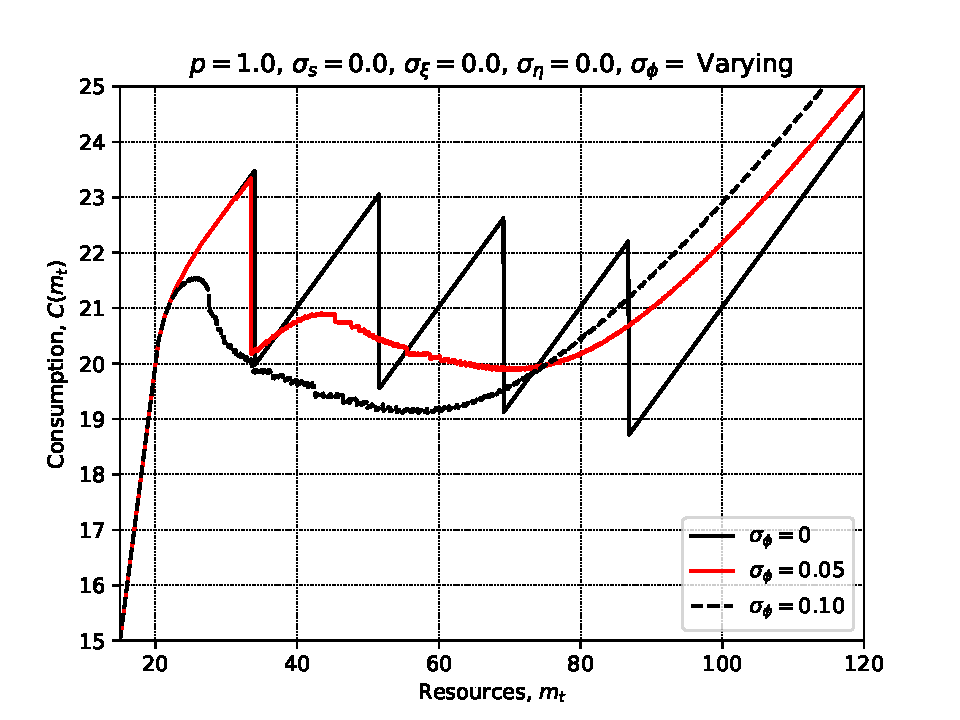
\includegraphics[width=\linewidth]{VaryPhi.pdf}
		\caption{Varying the price dispersion of retirement wealth.}
	\end{subfigure}
	\hfill
	\begin{subfigure}{0.48\textwidth}
		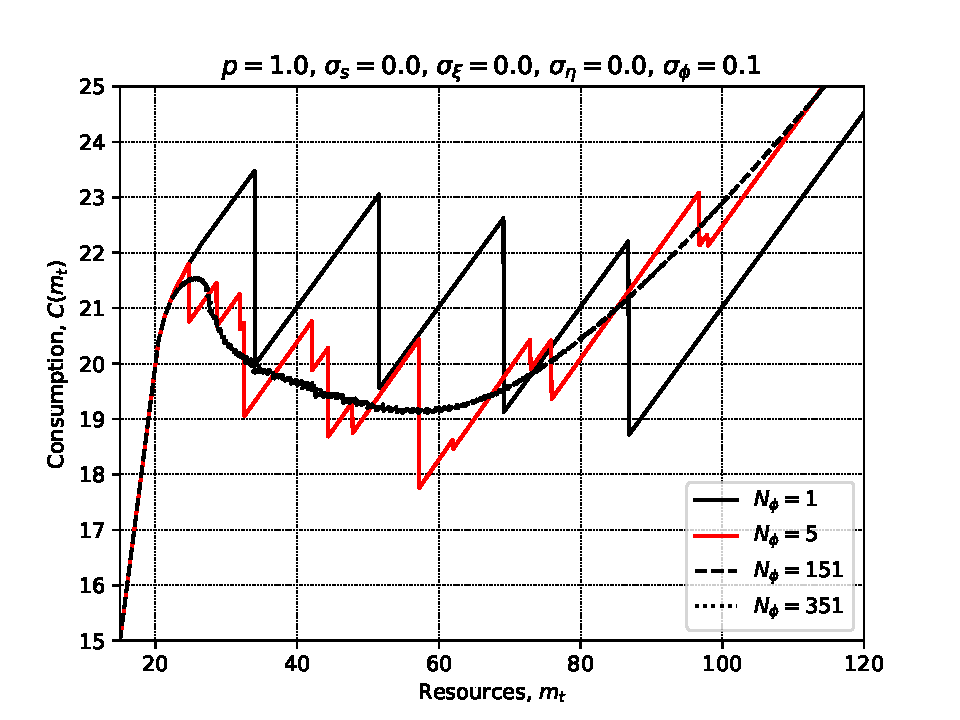
\includegraphics[width=\linewidth]{VaryPhiCount.pdf}
		\caption{Varying the number of price dispersion shock points.}
	\end{subfigure}
	\caption{The plots show the impact of increasing the smoothness through larger standard deviation of price dispersion
	(left panel) and increasing the number of price shock points (right panel).}
	\label{fig:fig8}
\end{figure}

Additionally, we can combine search with price dispersion. Since agents only receive a draw if they are searching, combining both methods amplifies the smoothing. Figure~\ref{fig:fig9} shows on the left that increasing search while keeping price dispersion small leads to a powerful smoothing mechanism. The right panel shows the opposite. When we keep search intensity as given, but increase price dispersion, the consumption function becomes very smooth and differentiable.

%---- Figure 9 ----
\begin{figure}[htbp]
	\centering
	\begin{subfigure}{0.48\textwidth}
		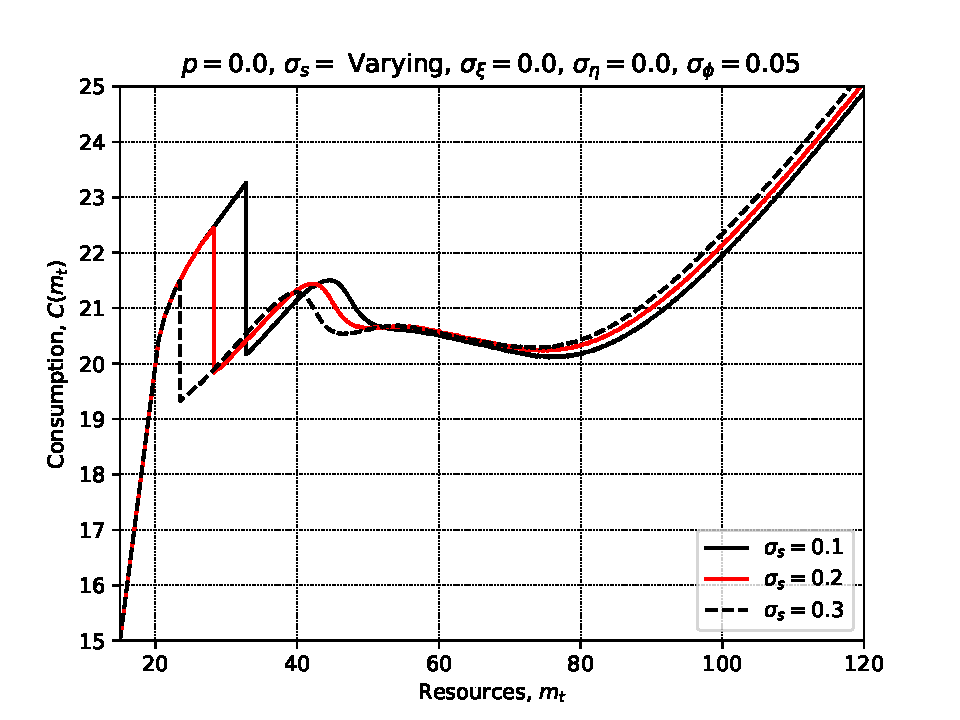
\includegraphics[width=\linewidth]{SearchPhi_VaryS.pdf}
		\caption{Varying the search intensity given price dispersion of retirement wealth.}
	\end{subfigure}
	\hfill
	\begin{subfigure}{0.48\textwidth}
		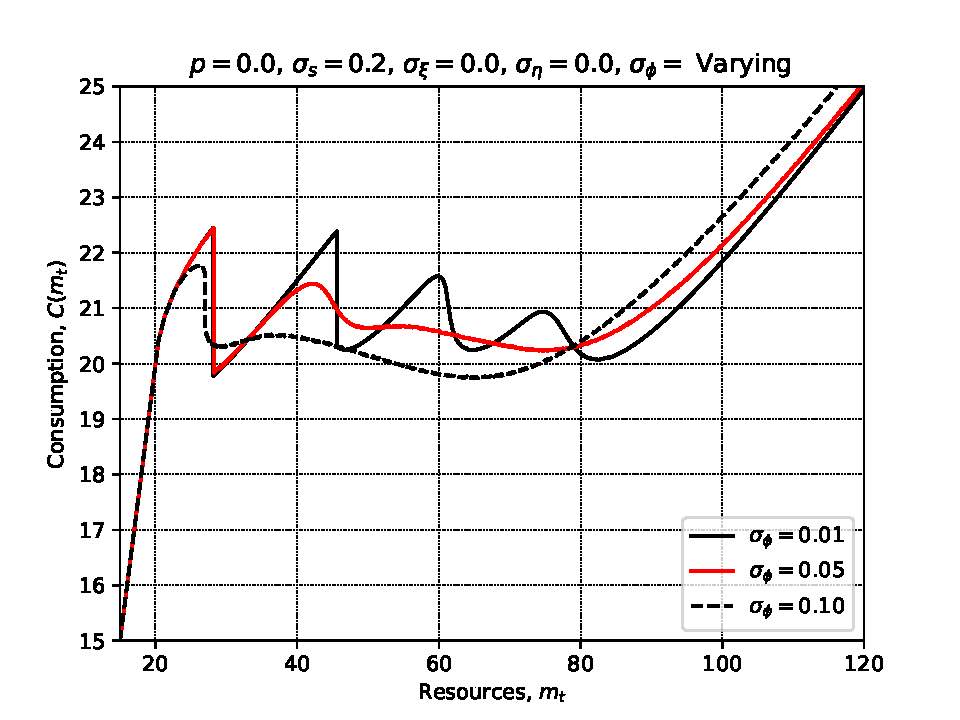
\includegraphics[width=\linewidth]{SearchPhi_VaryPhi.pdf}
		\caption{Varying price dispersion of retirement wealth given search intensity.}
	\end{subfigure}
	\caption{The plots show the impact of smoothness through the combination of search and price dispersion. Left panel keeps price dispersion fixed and varies search intensity and right panel keeps search intensity fixed and varies price dispersion.}
	\label{fig:fig9}
\end{figure}
\section{Durable model}\label{sec:DurableModel}

The second example is a consumption-savings model with durable and nondurable goods. It is a simplified version of the model in \cite{Monninger2025-cz} which uses endogeneous search as a numerical tool to solve the model. This section focuses on the solution method and compares the usage of taste shocks, endogeneous search, and stochastic durable prices.

\subsection{Model setup}\label{sec:ModelBasic}
The model consists of ex-ante identical agents who face uninsurable income risk and can consume non-durable goods, receive flow utility from a durable good, and can save in one single risk-free liquit asset.

\begin{figure}[h!]
	\centering
	\includegraphics[width=\textwidth]{timeline_DurableModel.pdf}
	\caption{Timeline of the durable model}
	\label{fig:timeline_DurableModel}
\end{figure}

The agent starts each period with beginning-of-period durable stock ($n_t$) and market resources ($m_t$). The agent solves the adjuster and keeper problems separately and chooses optimal levels of nondurable consumption $c_t$, durable stock $d_t$, and assets $a_t$. The discrete keep-versus-adjust decision is then resolved by a hard maximum over the two conditional value functions. At the end of the period, the agent holds a durable stock $d_t$ and liquid assets $a_t$. Between period $t$ and $t+1$, the transitory income shock materializes, interest is received, and the durable stock depreciates.

Each household is characterized by two state variables: beginning-of-period market resources $m_t$ and the stock of durables $n_t$. Preferences exhibit constant relative risk aversion and combine nondurable consumption $c_t$ and the service flow of durables $d_t$ using a Cobb-Douglas aggregator\footnote{Using this form is standard (eg see \cite{Berger2015-kp, McKay2021-ib}) which is in line with micro-evidence \cite{Berger2018-yb}. An alternative approach is to use a CES aggregator as in \cite{Mankiw1983-za}}:
\begin{align}
	u(c_t, d_t) &= \frac{\big(c_t^\alpha d_t^{1-\alpha}\big)^{1-\rho}}{1-\rho}, \qquad \alpha \in (0,1), \ \rho > 0.
\end{align}

At the start of the period, the household observes $(m_t, n_t)$ and decides whether to keep the durable stock unchanged or to adjust. If no adjustment occurs, the household sets $d_t = n_t$ and allocates $m_t$ between nondurable consumption and savings. If the household adjusts, it sells the entire beginning-of-period stock at no price risk but incurs a proportional adjustment cost $\tau \in (0,1)$. The resulting liquidity is
\begin{align}
	\ell_t = m_t + (1-\tau)n_t,
\end{align}
which can then be allocated across nondurable consumption, a new durable stock $d_t$, and savings $a_t$.

The household's problem is the hard discrete choice between keeping and adjusting:
\begin{align}
	v_t(m_t,n_t) = \max\Big\{ v_t^{\text{keep}}(m_t,n_t),\; v_t^{\text{adj}}(\ell_t)\Big\},
\end{align}
where $v_t^{\text{keep}}$ and $v_t^{\text{adj}}$ are the value functions conditional on keeping or adjusting.

Labor income is idiosyncratic and purely transitory. Normalized income is
\begin{align}
	y_t = \theta_t,
\end{align}
where $\theta_t$ is i.i.d.\ log-normally distributed with $\mathbb{E}[\theta_t] = 1$ and a strictly positive standard deviation. There is no unemployment risk.

Assets earn a single interest rate $r$, so the gross interest factor is $\mathcal{R} = 1+r$. The durable stock depreciates at rate $\delta \in (0,1)$. There are no maintenance costs and no operation costs. Therefore, next-period states evolve according to
\begin{align}
	m_{t+1} &= \mathcal{R} a_t + \theta_{t+1},\\
	n_{t+1} &= (1-\delta)\, d_t.
\end{align}

Borrowing is prohibited: the loan-to-value ratio is zero and the lower bound on assets is $\underline{a}=0$, so end-of-period assets must satisfy $a_t \ge 0$.

Hence, the Bellman equations conditional on keep and adjust are:
\begin{align}
	v_t^{\text{keep}}(m_t,n_t) &= \max_{c_t} \ u(c_t ,d_t) + \beta \mathbb{E}_t \big[ v_{t+1}(m_{t+1},n_{t+1}) \big],\\
	& \text{s.t. } a_t = m_t - c_t \geq 0,\\
	& \qquad d_t = n_t,\\
	& \qquad m_{t+1} = \mathcal{R} a_t + \theta_{t+1},\\
	& \qquad n_{t+1} = (1-\delta)\, d_t.\\[1em]
	v_t^{\text{adj}}(\ell_t) &= \max_{c_t,d_t} \ u(c_t,d_t) + \beta \mathbb{E}_t \big[ v_{t+1}(m_{t+1},n_{t+1}) \big],\\
	& \text{s.t. } a_t = \ell_t - c_t - d_t \geq 0,\\
	& \qquad m_{t+1} = \mathcal{R} a_t + \theta_{t+1},\\
	& \qquad n_{t+1} = (1-\delta)\, d_t.
\end{align}

With the following first-order conditions with respect to nondurable consumption and durable stock:
\begin{align}
	\frac{\partial v_t^{adj}}{\partial c_t} &= u_c(c_t, d_t) \geq \beta \mathcal{R}\, \mathbb{E}_t \big[v_{t+1}^m\big], \label{eq:FOC_c_basic} \\
	\frac{\partial v_t^{adj}}{\partial d_t} &= u_d(c_t, d_t) \geq \beta \mathcal{R}\, \mathbb{E}_t\big[v_{t+1}^m\big] - \beta (1 - \delta)\, \mathbb{E}_t\big[v_{t+1}^n\big], \label{eq:FOC_d_basic}
\end{align}

Equations~\ref{eq:FOC_c_basic} and~\ref{eq:FOC_d_basic} are stated as KKT conditions. Equality holds when the borrowing constraint does not bind, and the left-hand side strictly exceeds the right-hand side when it does. Equation~\ref{eq:FOC_c_basic} equates the marginal utility of nondurable consumption with the discounted shadow value of savings. Equation~\ref{eq:FOC_d_basic} shows that the marginal utility of durables equals the net user cost: the first term on the right is the discounted opportunity cost $\mathcal{R}$ of diverting a unit of resources into durables rather than liquid assets, and the second term is the discounted benefit of carrying the remaining durable stock $(1-\delta)d_t$ into the next period.

\subsection{Algorithm}\label{subsec:AlgorithmBasic}
This section outlines the algorithm for one recursive period of the baseline model: no Extreme Value Type~I taste shocks, no directed search, and no durable-price dispersion. The discrete keep-versus-adjust choice is resolved by a hard maximum. The terminal period is closed form---the keeper sets $c_T=m_T$ and $d_T=n_T$, the adjuster sets $c_T=\alpha\ell_T$ and $d_T=(1-\alpha)\ell_T$, and the two branches are combined by a hard max---so Algorithm~\ref{alg:durable_baseline} starts from a given next-period solution $(v_{t+1},\,v_{t+1}^{m},\,v_{t+1}^{n})$.

Define the end-of-period (gothic) objects on $(d_t,a_t)$ by
\begin{align}
	\mathfrak{v}_c'(d_t,a_t) &= \beta\,\mathcal{R}\,\mathbb{E}_t\big[v_{t+1}^{m}(n_{t+1},m_{t+1})\big],\\
	\mathfrak{v}_d'(d_t,a_t) &= \beta\,(1-\delta)\,\mathbb{E}_t\big[v_{t+1}^{n}(n_{t+1},m_{t+1})\big],\\
	\mathfrak{v}(d_t,a_t) &= \beta\,\mathbb{E}_t\big[v_{t+1}(n_{t+1},m_{t+1})\big],
\end{align}
with $m_{t+1}=\mathcal{R}a_t+\theta_{t+1}$ and $n_{t+1}=(1-\delta)d_t$. The expectation over $\theta_{t+1}$ may be evaluated by quadrature (as written below) or by the transition-matrix integration described in Appendix~\ref{sec:appdx_model_basic}. Because adjustment costs make the first-order conditions only necessary, the keeper step applies a DC-EGM upper envelope \citep{Iskhakov2017-jb} and the adjuster step applies FUES \citep{Dobrescu2022-ii}.

\begin{algorithm}[htbp]
\caption{EGM step for the baseline durable model (hard max)}
\label{alg:durable_baseline}
\DontPrintSemicolon
Let $\vec{\theta}=\{\theta_1,\dots,\theta_J\}$ be quadrature points for the transitory income shock with weights $\vec{\omega}=\{\omega_1,\dots,\omega_J\}$.\;
Form ascending grids $\vec{a}_t=\{a^1,\dots,a^I\}$, $\vec{d}_t=\{d^1,\dots,d^L\}$, a fine durable grid $\vec{d}_t^{\mathrm{adj}}$ for the adjuster FOC scan, and beginning-of-period grids $\vec{n}_t$, $\vec{m}_t$.\;
\BlankLine
\tcc{End-of-period (gothic) functions}
\For{$i = 1,\dots,I$}{
	\For{$q = 1,\dots,L$}{
		\For{$j = 1,\dots,J$}{
			Compute $m_{t+1}^{j}(a^i)=\mathcal{R}a^i+\theta_j$ and $n_{t+1}(d^q)=(1-\delta)d^q$\;
			Interpolate $v_{t+1}$, $v_{t+1}^{m}$, and $v_{t+1}^{n}$ at $(n_{t+1}(d^q),\,m_{t+1}^{j}(a^i))$\;
		}
		Compute $\mathfrak{v}_c'(d^q,a^i)=\beta\mathcal{R}\sum_{j=1}^{J}\omega_j\,v_{t+1}^{m}(n_{t+1}(d^q),m_{t+1}^{j}(a^i))$\;
		Compute $\mathfrak{v}_d'(d^q,a^i)=\beta(1-\delta)\sum_{j=1}^{J}\omega_j\,v_{t+1}^{n}(n_{t+1}(d^q),m_{t+1}^{j}(a^i))$\;
		Compute $\mathfrak{v}(d^q,a^i)=\beta\sum_{j=1}^{J}\omega_j\,v_{t+1}(n_{t+1}(d^q),m_{t+1}^{j}(a^i))$\;
	}
}
\BlankLine
\tcc{Keeper: EGM with $d_t=n_t$, then DC-EGM upper envelope}
\For{each $n\in\vec{n}_t$}{
	\For{$i = 1,\dots,I$}{
		Compute $c_t^{\mathrm{keep}}(a^i;n)=u_c^{-1}\big(\mathfrak{v}_c'(n,a^i);\,n\big)$\;
		Compute endogenous resources $m_t^{\mathrm{EGM}}(a^i;n)=a^i+c_t^{\mathrm{keep}}(a^i;n)$\;
		Compute $v_t^{\mathrm{EGM}}(a^i;n)=u\big(c_t^{\mathrm{keep}}(a^i;n),n\big)+\mathfrak{v}(n,a^i)$\;
	}
	Apply a DC-EGM upper envelope to $\{(m_t^{\mathrm{EGM}},\,c_t^{\mathrm{keep}},\,v_t^{\mathrm{EGM}})\}$ and interpolate onto $\vec{m}_t$ to obtain $c_t^{\mathrm{keep}}(n,m)$, $a_t^{\mathrm{keep}}=\max\{m-c_t^{\mathrm{keep}},0\}$, and $d_t^{\mathrm{keep}}=n$\;
	Compute $v_t^{\mathrm{keep}}(n,m)=u(c_t^{\mathrm{keep}},n)+\mathfrak{v}(n,a_t^{\mathrm{keep}})$, $v_t^{m,\mathrm{keep}}=u_c(c_t^{\mathrm{keep}},n)$, and $v_t^{n,\mathrm{keep}}=u_d(c_t^{\mathrm{keep}},n)+\mathfrak{v}_d'(n,a_t^{\mathrm{keep}})$\;
}
\BlankLine
\tcc{Adjuster: FOC roots in $a$ on a fine $d$-grid, then FUES in liquidity}
Initialize empty candidate clouds for $(\ell_t,c_t,d_t,a_t,v_t)$\;
\For{each $d\in\vec{d}_t^{\mathrm{adj}}$}{
	Find all roots $a$ of $u_d(c,d)-\mathfrak{v}_c'(d,a)+\mathfrak{v}_d'(d,a)=0$ with $c=u_c^{-1}\big(\mathfrak{v}_c'(d,a);\,d\big)$\;
	\For{each root $a$}{
		Compute $\ell_t=a+c+d$ and $v_t^{\mathrm{adj}}=u(c,d)+\mathfrak{v}(d,a)$\;
		Append $(\ell_t,c,d,a,v_t^{\mathrm{adj}})$ to the candidate cloud\;
	}
}
Sort candidates by $\ell_t$ and apply FUES to obtain refined points $(\ell_t,c_t^{\mathrm{adj}},d_t^{\mathrm{adj}},a_t^{\mathrm{adj}},v_t^{\mathrm{adj}})$\;
Construct one-dimensional interpolants $c_t^{\mathrm{adj}}(\ell)$, $d_t^{\mathrm{adj}}(\ell)$, and $a_t^{\mathrm{adj}}(\ell)$\;
\For{each $(n,m)\in\vec{n}_t\times\vec{m}_t$}{
	Compute $\ell_t=m+(1-\tau)n$\;
	Evaluate $c_t^{\mathrm{adj}}(\ell_t)$, $d_t^{\mathrm{adj}}(\ell_t)$, and $a_t^{\mathrm{adj}}=\max\{\ell_t-c_t^{\mathrm{adj}}-d_t^{\mathrm{adj}},0\}$\;
	Compute $v_t^{\mathrm{adj}}(\ell_t)=u(c_t^{\mathrm{adj}},d_t^{\mathrm{adj}})+\mathfrak{v}(d_t^{\mathrm{adj}},a_t^{\mathrm{adj}})$, $v_t^{m,\mathrm{adj}}=u_c(c_t^{\mathrm{adj}},d_t^{\mathrm{adj}})$, and $v_t^{n,\mathrm{adj}}=(1-\tau)\,u_c(c_t^{\mathrm{adj}},d_t^{\mathrm{adj}})$\;
}
\BlankLine
\tcc{Hard-max discrete choice}
\For{each $(n,m)\in\vec{n}_t\times\vec{m}_t$}{
	Set $\mathcal{I}_t(n,m)=1$ if $v_t^{\mathrm{adj}}\big(m+(1-\tau)n\big)\ge v_t^{\mathrm{keep}}(n,m)$ and $0$ otherwise\;
	Set $(c_t,d_t,a_t,v_t,v_t^{m},v_t^{n})$ to the adjuster branch if $\mathcal{I}_t=1$ and to the keeper branch if $\mathcal{I}_t=0$\;
}
Collect the combined policies and (inverse) value functions on $(\vec{n}_t,\vec{m}_t)$ for use in period $t-1$.\;
\end{algorithm}

\subsection{Illustration of the numerical challenge}

Fig.~\ref{fig:baseline_T} illustrates the terminal solution. Taking the hard-max between the options of adjusting and keeping, the S,s structure emerges (fig.~\ref{fig:baseline_ss_T}) which leads to a sharp switch between fully adjusting or fully keeping. As a result, the optimal policy functions of the model conditional on adjusting and keeping experience discontinuities along the switchpoints as illustrated for the durable consumption function (fig.~\ref{fig:baseline_d_T}).

\begin{figure}[htbp]
	\centering
	\begin{subfigure}{0.48\textwidth}
		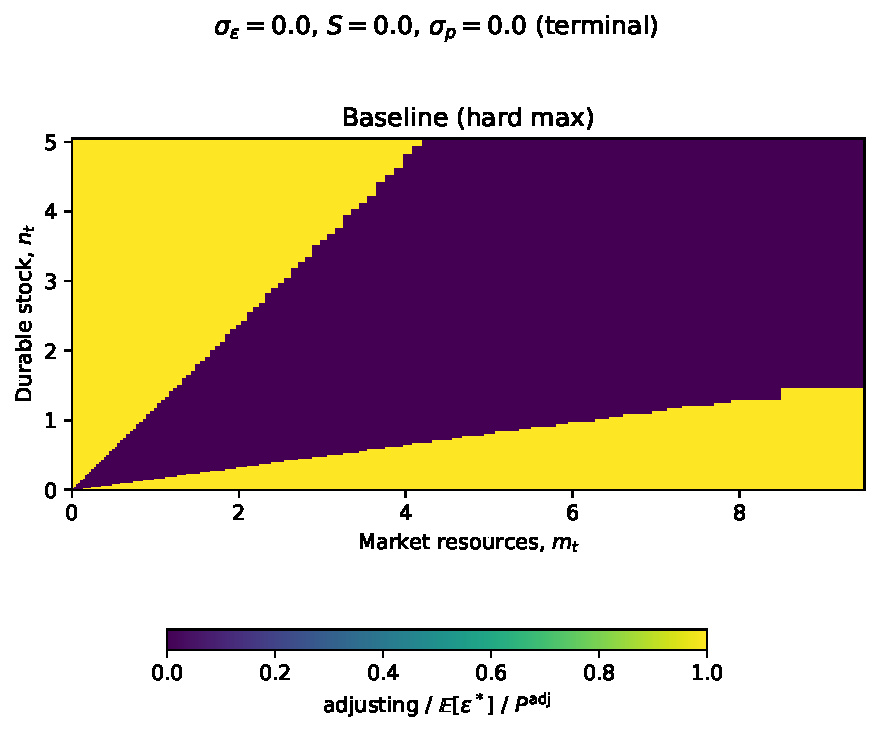
\includegraphics[width=\linewidth]{../../Figures/DurableModel/Baseline_Ss_T.pdf}
		\caption{Adjustment region (S,s bands).}
		\label{fig:baseline_ss_T}
	\end{subfigure}
	\hfill
	\begin{subfigure}{0.48\textwidth}
		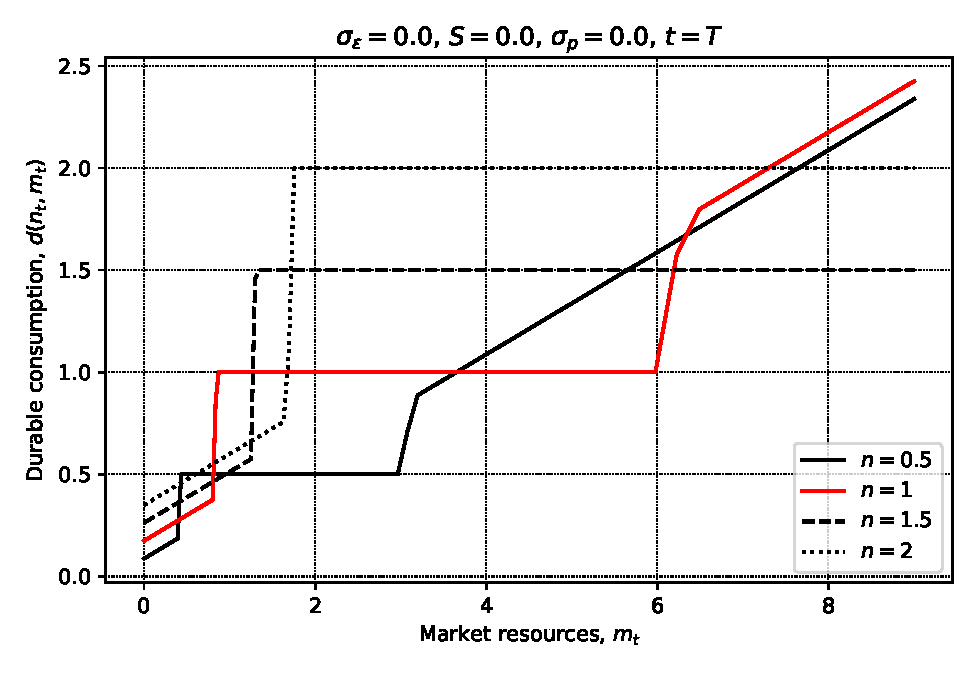
\includegraphics[width=\linewidth]{../../Figures/DurableModel/Baseline_d_T.pdf}
		\caption{Durable policy $d_t(n_t,m_t)$.}
		\label{fig:baseline_d_T}
	\end{subfigure}
	\vspace{0.5em}
	\begin{subfigure}{0.48\textwidth}
		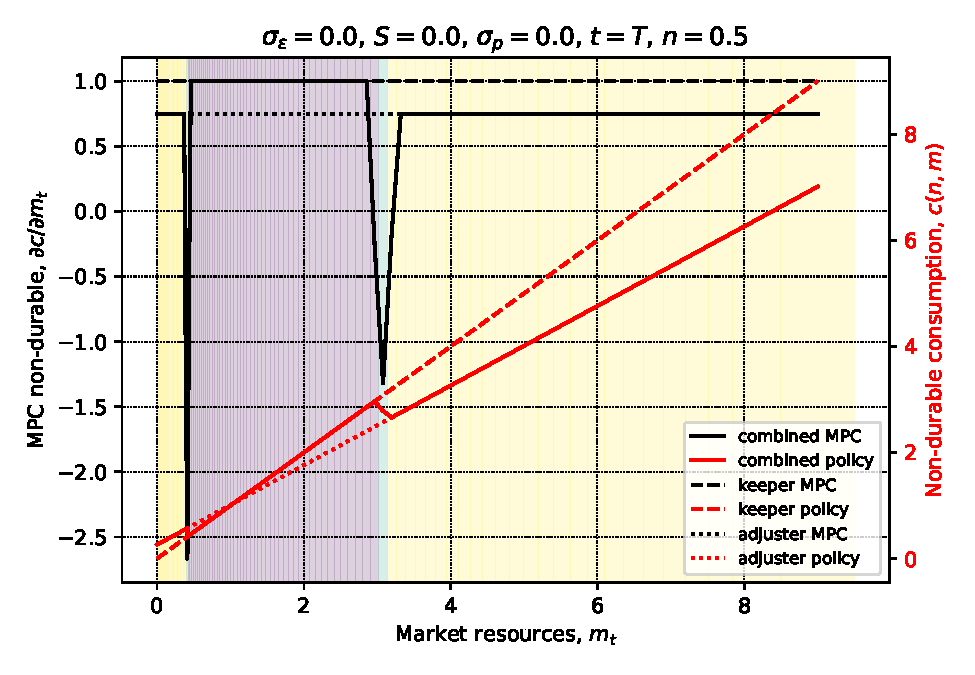
\includegraphics[width=\linewidth]{../../Figures/DurableModel/Baseline_c_T_MPC_decomp.pdf}
		\caption{MPC decomposition of nondurable consumption $c_t(n_t,m_t)$.}
		\label{fig:baseline_c_T_MPC_decomp}
	\end{subfigure}
	\hfill
	\begin{subfigure}{0.48\textwidth}
		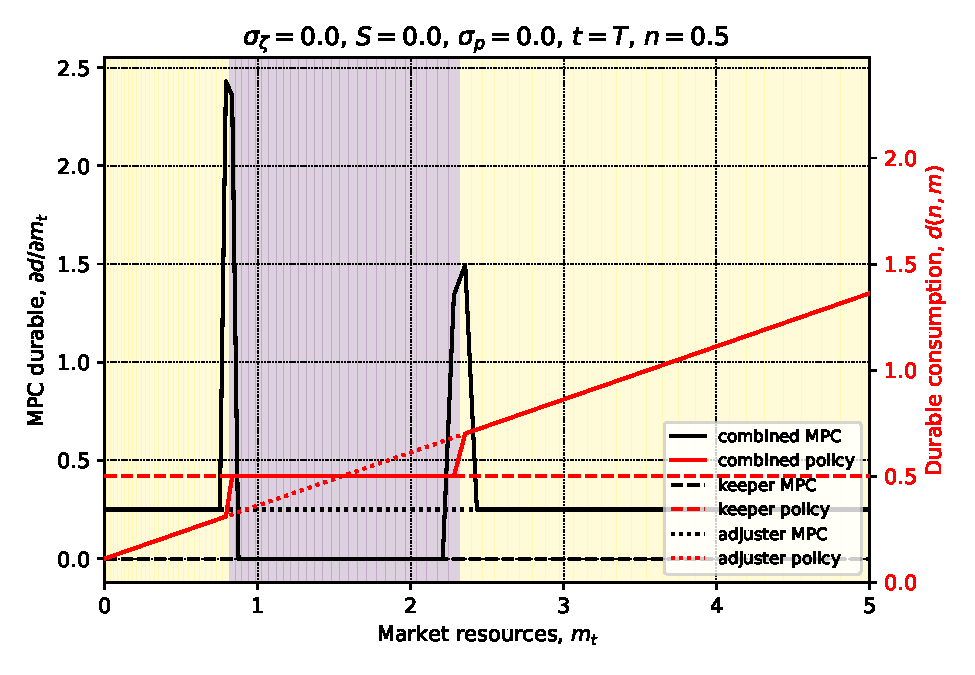
\includegraphics[width=\linewidth]{../../Figures/DurableModel/Baseline_d_T_MPC_decomp.pdf}
		\caption{MPC decomposition of durable consumption $d_t(n_t,m_t)$.}
		\label{fig:baseline_d_T_MPC_decomp}
	\end{subfigure}
	\caption{Terminal-period solution of the baseline durable model (hard max). The upper left panel shows the keep--adjust regions in $(m_t,n_t)$ space; the upper right panel shows the combined durable policy for selected beginning-of-period durable stocks $n_t$. The lower panels show the MPC decomposition of nondurable and durable consumption given a fixed beginning-of-period durable stock $n_t$.}
	\label{fig:baseline_T}
\end{figure}
	
	
In earlier periods, the agent incorporates the switchpoints in the next period into the solution of today's problem. Together with non-convex adjustment costs, the first order conditions are only necessary, but not sufficient. Hence, we need to incorporate an upper envelope algorithm such as FUES. However, even with this algorithm, small discontinuities still arise in the adjuster policy functions. Additionally, by combining the keeper and adjuster functions each period, these non-convexities propagade backwards similar to the retirement problem. Figure~\ref{fig:baseline_t_MPC_decomp} illustrates this for a fixed beginning-of-period durable stock $n_t$. In the yellow adjuster region, the policy function and MPC follows the adjuster policy function. With higher market resources, the S,s border gets crossed resulting in stark spikes in MPCs.

\begin{figure}[htbp]
	\centering
	\begin{subfigure}{0.48\textwidth}
		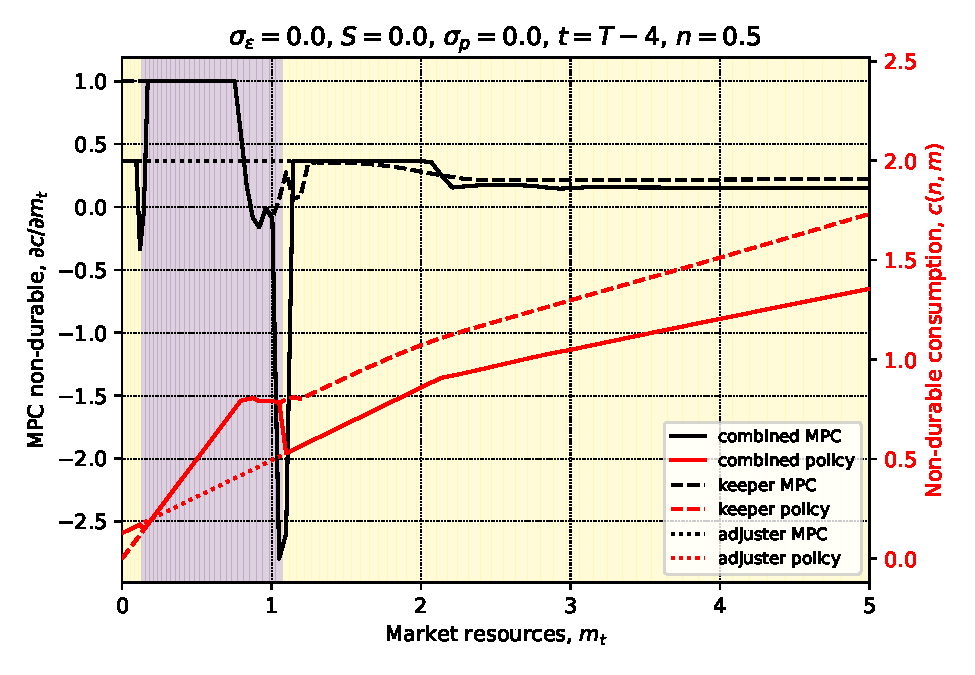
\includegraphics[width=\linewidth]{../../Figures/DurableModel/Baseline_c_periodt_MPC_decomp.pdf}
		\caption{MPC decomposition of nondurable consumption $c_t(n_t,m_t)$.}
		\label{fig:baseline_c_periodt_MPC_decomp}
	\end{subfigure}
	\hfill
	\begin{subfigure}{0.48\textwidth}
		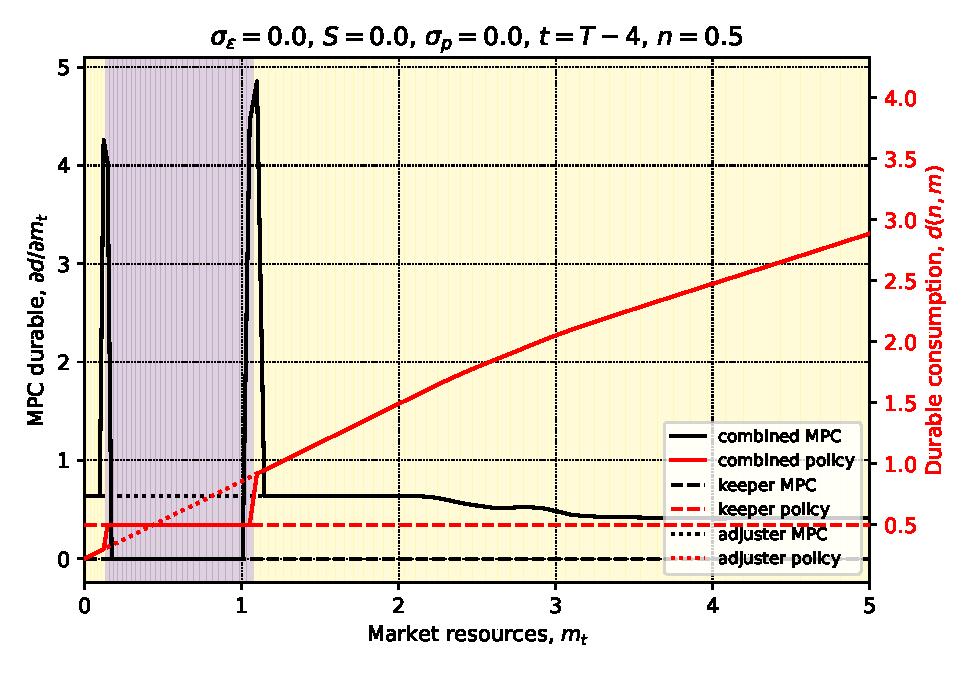
\includegraphics[width=\linewidth]{../../Figures/DurableModel/Baseline_d_periodt_MPC_decomp.pdf}
		\caption{MPC decomposition of durable consumption $d_t(n_t,m_t)$.}
		\label{fig:baseline_d_periodt_MPC_decomp}
	\end{subfigure}
	\caption{MPC and policy functions of non-durable and durable consumption.}
	\label{fig:baseline_t_MPC_decomp}
\end{figure}
\subsection{Extension: Extreme Value Type I Taste Shocks}\label{subsec:ModelBasicTaste}

The hard maximum in the discrete keep-versus-adjust decision produces a kink in the value function and a discontinuity in the policy functions at the state combinations $(m_t,n_t)$ where the household is indifferent between the two branches. Following the discrete--continuous choice literature (e.g.\ \cite{Iskhakov2017-jb}), this subsection smooths that discontinuity with i.i.d.\ Extreme Value Type I (Gumbel) taste shocks on the two discrete alternatives, while leaving search frictions aside (these are introduced separately in Section~\ref{subsec:ModelBasicSearch}). Unlike the multiplicative mean-one log-normal taste shocks used in the retirement application of Section~\ref{sec:RetirementModel}, EV Type I shocks enter \emph{additively} on each branch and are integrated out in closed form: they randomize the discrete outcome directly through logit choice probabilities, without introducing an additional continuous (or discretized) state.

At the start of period $t$, after observing $(m_t,n_t)$, the household draws i.i.d.\ Extreme Value Type I shocks $(\varepsilon_t^{\text{keep}},\varepsilon_t^{\text{adj}})$ and chooses the branch that maximizes the shock-augmented conditional value,
\begin{align}
	v_t(m_t,n_t)
	&= \max\Big\{
		v_t^{\text{keep}}(m_t,n_t) + \sigma_\varepsilon\,\varepsilon_t^{\text{keep}},\;
		v_t^{\text{adj}}(\ell_t) + \sigma_\varepsilon\,\varepsilon_t^{\text{adj}}
	\Big\}, \label{eq:taste_discrete_EV}
\end{align}
where $\sigma_\varepsilon > 0$ is the taste-shock scale and $\ell_t = m_t+(1-\tau)n_t$. The conditional value functions $v_t^{\text{keep}}(m_t,n_t)$ and $v_t^{\text{adj}}(\ell_t)$ retain exactly the same Bellman definitions as in the baseline model: the taste shocks do not enter the inner continuous maximizations, so the first-order conditions~\eqref{eq:FOC_c_basic}--\eqref{eq:FOC_d_basic} and the continuous policies $c_t^{\text{keep}}$, $c_t^{\text{adj}}$, $d_t^{\text{adj}}$ are unchanged.

Because $(\varepsilon_t^{\text{keep}},\varepsilon_t^{\text{adj}})$ are i.i.d.\ Extreme Value Type I, the expectation of~\eqref{eq:taste_discrete_EV} has the closed-form log-sum representation
\begin{align}
	v_t(m_t,n_t)
	&= \sigma_\varepsilon \log\Big(
		\exp\big(v_t^{\text{keep}}(m_t,n_t)/\sigma_\varepsilon\big)
		+ \exp\big(v_t^{\text{adj}}(\ell_t)/\sigma_\varepsilon\big)
	\Big), \label{eq:taste_logsum}
\end{align}
with logit choice probabilities
\begin{align}
	P_t^{\text{adj}}(m_t,n_t)
	&= \frac{\exp\big(v_t^{\text{adj}}(\ell_t)/\sigma_\varepsilon\big)}
	{\exp\big(v_t^{\text{keep}}(m_t,n_t)/\sigma_\varepsilon\big)
	+ \exp\big(v_t^{\text{adj}}(\ell_t)/\sigma_\varepsilon\big)},
	\qquad
	P_t^{\text{keep}}(m_t,n_t) = 1 - P_t^{\text{adj}}(m_t,n_t). \label{eq:taste_logit}
\end{align}
The expected (ex-ante) policy functions are the probability-weighted averages of the two branches,
\begin{align}
	c_t(m_t,n_t) &= P_t^{\text{keep}}\, c_t^{\text{keep}}(m_t,n_t) + P_t^{\text{adj}}\, c_t^{\text{adj}}(\ell_t), \label{eq:taste_c_combined}\\
	d_t(m_t,n_t) &= P_t^{\text{keep}}\, n_t + P_t^{\text{adj}}\, d_t^{\text{adj}}(\ell_t). \label{eq:taste_d_combined}
\end{align}
As $\sigma_\varepsilon \to 0$, the logit probabilities collapse to the hard indicators of the baseline model and~\eqref{eq:taste_logsum} collapses to the hard maximum. Larger $\sigma_\varepsilon$ spreads probability mass onto the inferior branch near indifference, so $c_t$ and $d_t$ (and the marginal-value functions derived from the inclusive value~\eqref{eq:taste_logsum}) are smooth in $(m_t,n_t)$. No quadrature over taste nodes is required: the EV Type I assumption delivers the inclusive value and choice probabilities in closed form. The taste shocks do not alter the household's budget set, so the no-borrowing constraint $a_t \ge 0$ is unaffected. I derive the envelope conditions, the Euler equations, and the EGM algorithm with EV Type I taste shocks in appendix~\ref{subsec:appdx_taste_basic}.

As a result, the S,s curve in the terminal period is smoothened and adjuster values between zero and one are optimal. In the aggregate, the policy functions are a convex combination of adjuster and keeper policy functions around the S,s thresholds. Fig~\ref{fig:tasteshock_T} illustrates the point clearly.

\begin{figure}[htbp]
	\centering
	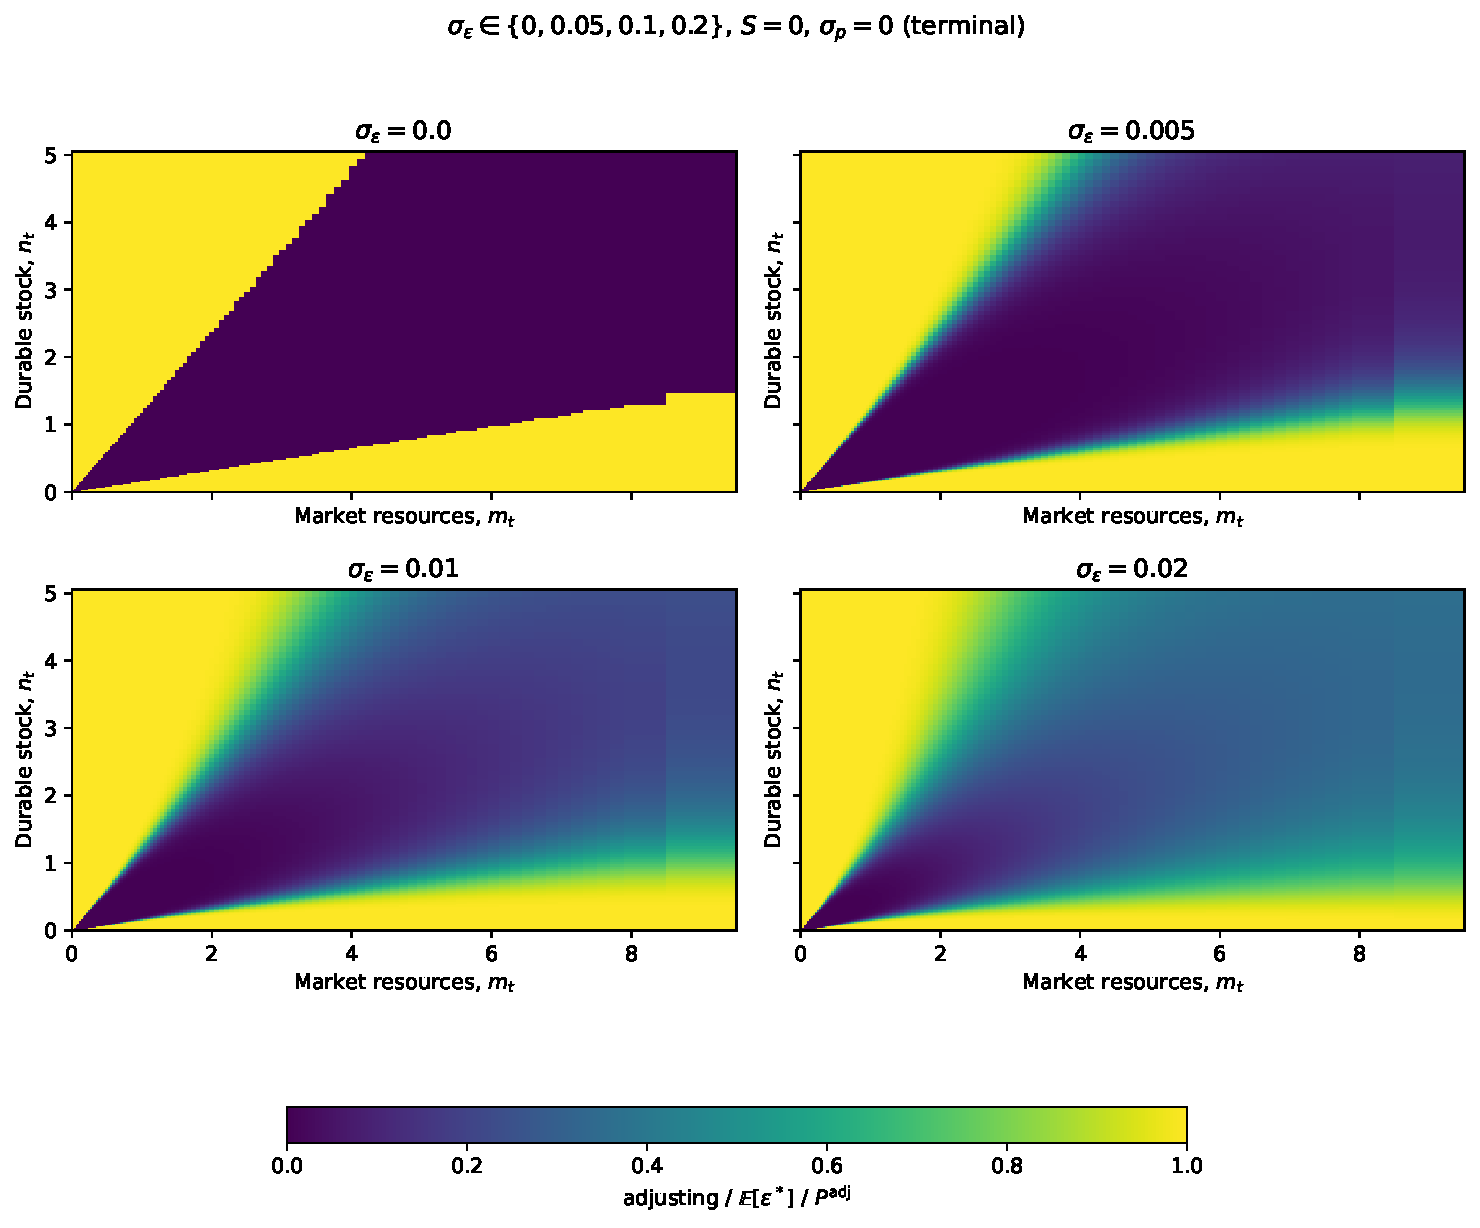
\includegraphics[width=\linewidth]{../../Figures/DurableModel/TasteShock_Ss_T.pdf}
	\caption{Terminal-period keep--adjust regions in $(m_t,n_t)$ space under EV Type I taste shocks for $\sigma_\varepsilon \in \{0, 0.05, 0.1, 0.2\}$.}
	\label{fig:tasteshock_ss_T}
	\label{fig:tasteshock_T}
\end{figure}

As a result, the discontinuities in period t disapear with a small EV shock parameter. Fig~\ref{fig:tasteshock_periodt_MPC_decomp} show the now continuous consumption functions and marginal propensities to consume and expend.


\begin{figure}[htbp]
	\centering
	\begin{subfigure}{0.48\textwidth}
		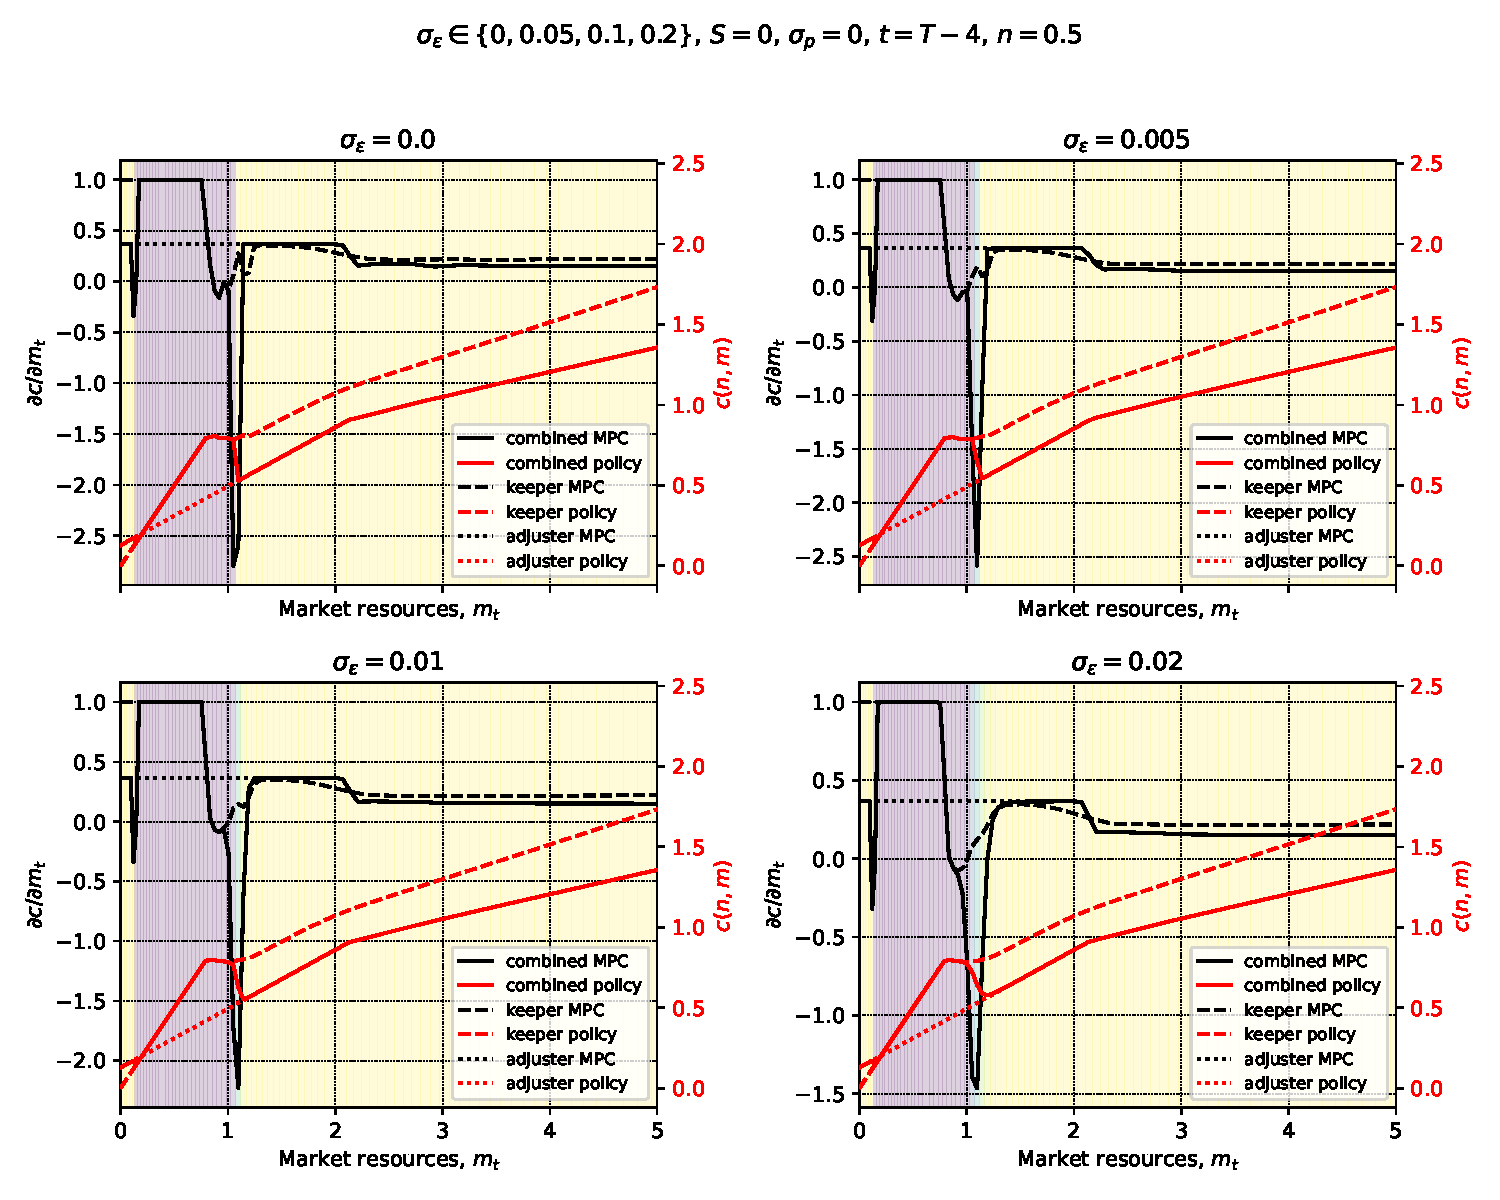
\includegraphics[width=\linewidth]{../../Figures/DurableModel/TasteShock_c_periodt_MPC_decomp.pdf}
		\caption{MPC decomposition of nondurable consumption $c_t(n_t,m_t)$.}
		\label{fig:tasteshock_c_periodt_MPC_decomp}
	\end{subfigure}
	\hfill
	\begin{subfigure}{0.48\textwidth}
		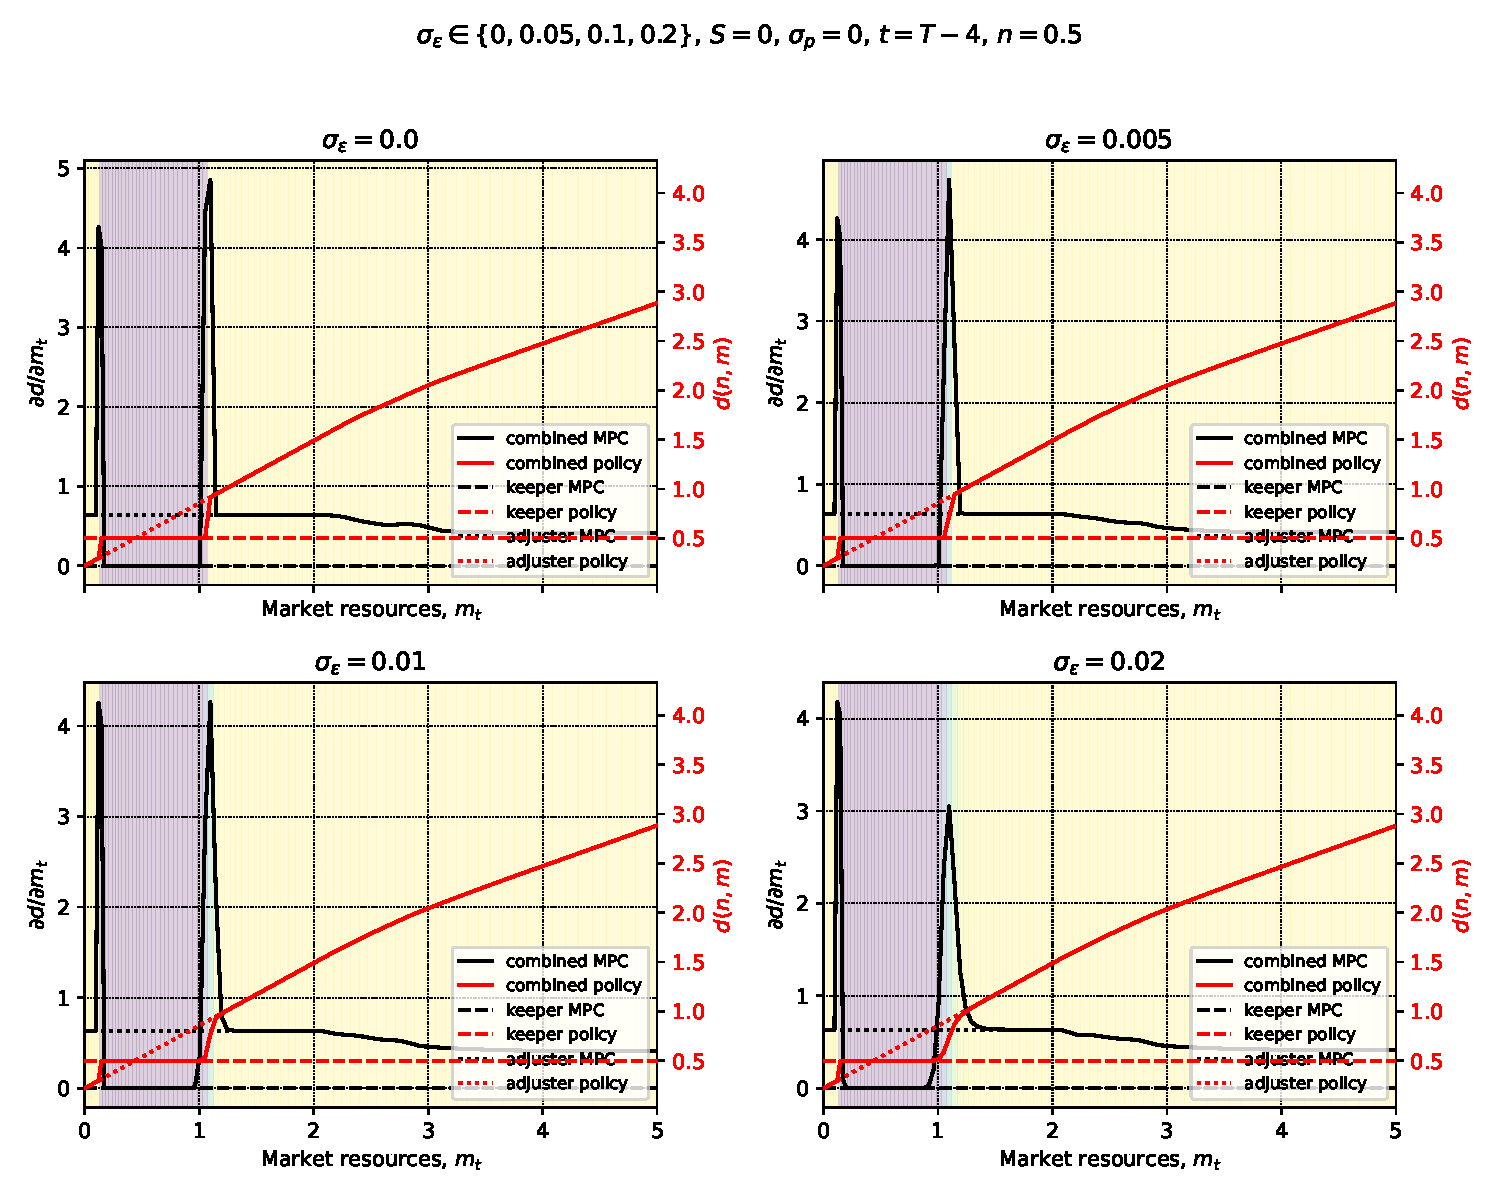
\includegraphics[width=\linewidth]{../../Figures/DurableModel/TasteShock_d_periodt_MPC_decomp.pdf}
		\caption{MPC decomposition of durable consumption $d_t(n_t,m_t)$.}
		\label{fig:tasteshock_d_periodt_MPC_decomp}
	\end{subfigure}
	\caption{MPC and policy functions of non-durable and durable consumption using EV taste shocks.}
	\label{fig:tasteshock_periodt_MPC_decomp}
\end{figure}

\subsection{Extension: Search Frictions}\label{subsec:ModelBasicSearch}

This subsection instead reintroduces the directed-search mechanism of the full model into the basic environment, without taste shocks. Rather than resolving the keep-versus-adjust margin with a hard maximum, the household chooses a search intensity $\varepsilon_t \in [0,1]$ that determines the weight placed on the adjuster's conditional value in the current period. Exerting search effort is costly, with cost function
\begin{align}
	\sigma(\varepsilon_t) = S\big[\varepsilon_t + (1-\varepsilon_t)\log(1-\varepsilon_t)\big], \label{eq:search_cost_basic}
\end{align}
where $S>0$ governs the degree of friction in the market for durables, following \cite{Khan2019-ew}. The beginning-of-period problem becomes
\begin{align}
	v_t(m_t,n_t) = \max_{\varepsilon_t \in [0,1]} \Big[(1-\varepsilon_t)\, v_t^{\text{keep}}(m_t,n_t) + \varepsilon_t\, v_t^{\text{adj}}(\ell_t) - \sigma(\varepsilon_t)\Big], \label{eq:search_discrete_basic}
\end{align}
where $v_t^{\text{keep}}$ and $v_t^{\text{adj}}$ retain exactly the same Bellman definitions as in the baseline model, except that the continuation value $v_{t+1}(m_{t+1},n_{t+1})$ appearing inside them is now itself given recursively by equation~\eqref{eq:search_discrete_basic} one period ahead, rather than by the hard maximum of the baseline model. All other features of the basic environment---the single interest rate $\mathcal{R}$, the absence of maintenance costs, and the no-borrowing constraint $a_t \ge 0$---are unchanged.

Search effort is chosen before the discrete outcome is known: $\varepsilon_t$ can be interpreted as the probability with which the household successfully locates a suitable durable this period, so the combined value function~\eqref{eq:search_discrete_basic} is a probability-weighted average of the two conditional values, net of the search cost. As $S \to 0$, search becomes costless, the household sets $\varepsilon_t \in \{0,1\}$, and the model collapses to the hard-maximum baseline; as $S \to \infty$, search becomes prohibitively costly, $\varepsilon_t^\ast \to 0$, and the household never adjusts. I derive the optimal search-effort rule, the smooth combined marginal-value functions, and the associated EGM steps in appendix~\ref{subsec:appdx_search_basic}.

Endogeneous search achieves a similar smoothing compared to the EV shocks. Fig~\ref{fig:search_ss_T} illustrates the terminal period solution. A small search cost is sufficient to lead to a smoothened S,s region.

\begin{figure}[htbp]
	\centering
	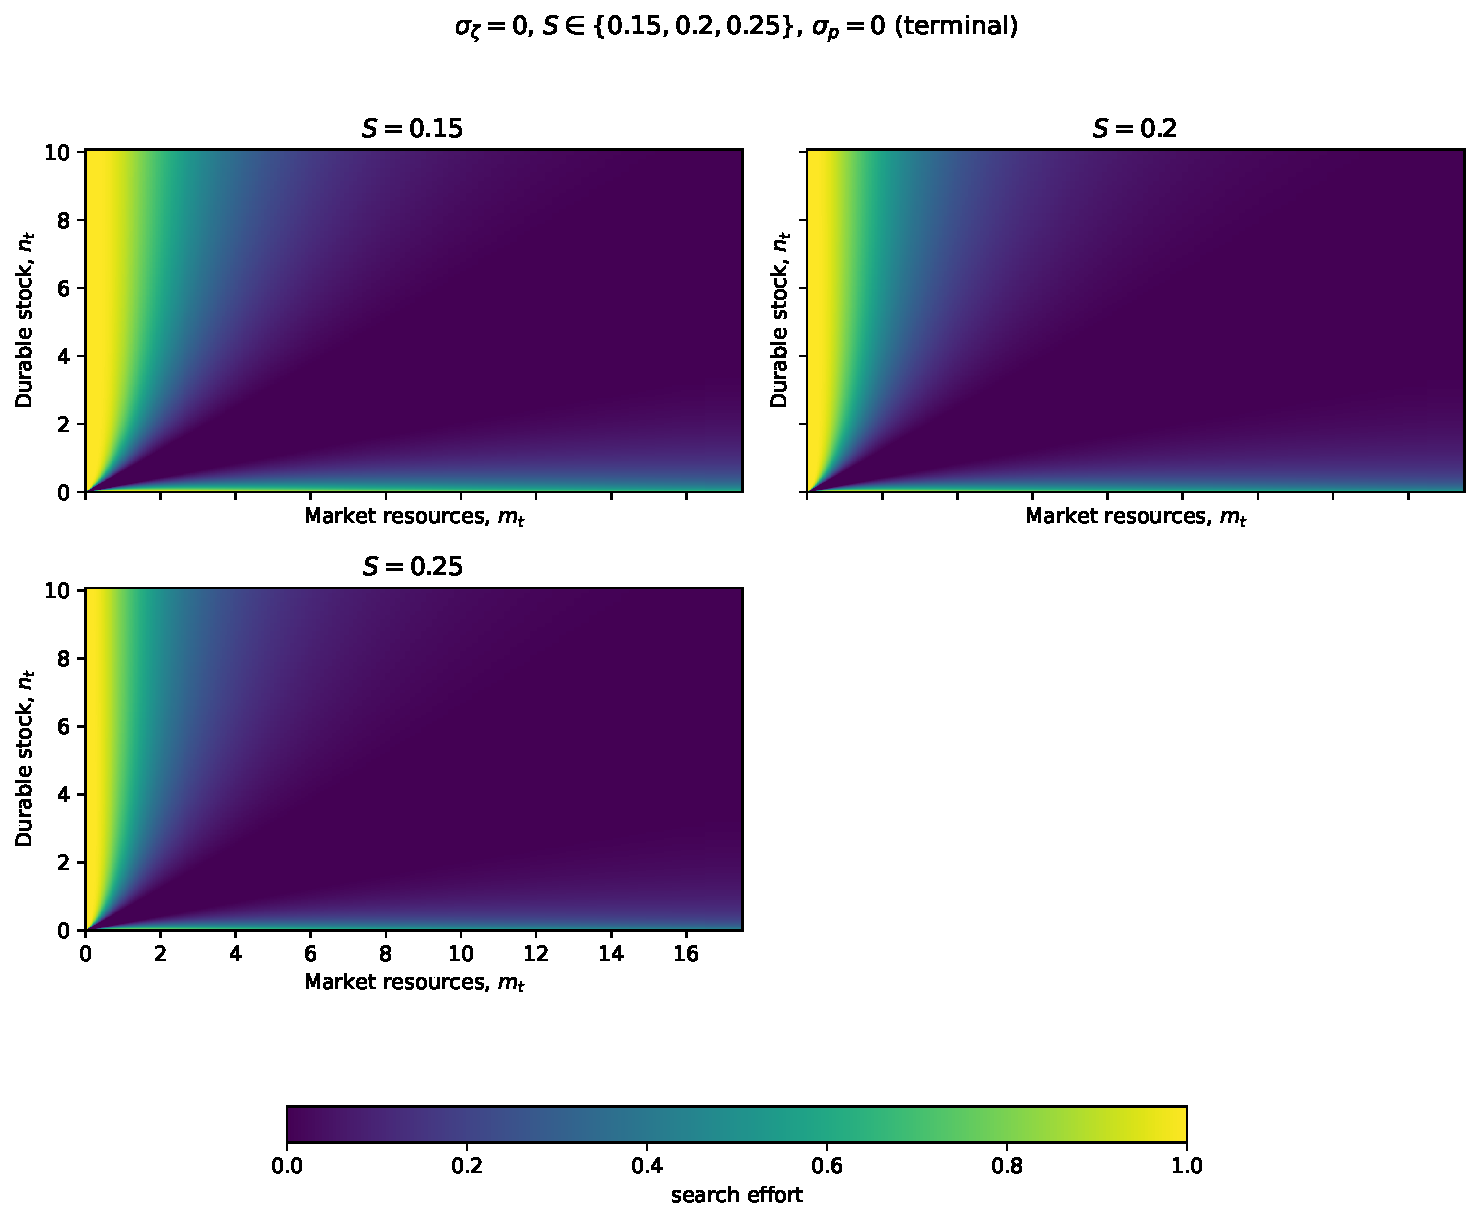
\includegraphics[width=\linewidth]{../../Figures/DurableModel/Search_Ss_T.pdf}
	\caption{Terminal-period keep--adjust regions in $(m_t,n_t)$ space under endogeneous search for search-cost scales $S \in \{0, 0.05, 0.1, 0.2\}$.}
	\label{fig:search_ss_T}
\end{figure}

As a result, optimal consumption functions in period t are smooth as well (see fig~\ref{fig:search_periodt_MPC_decomp}).

\begin{figure}[htbp]
	\centering
	\begin{subfigure}{0.48\textwidth}
		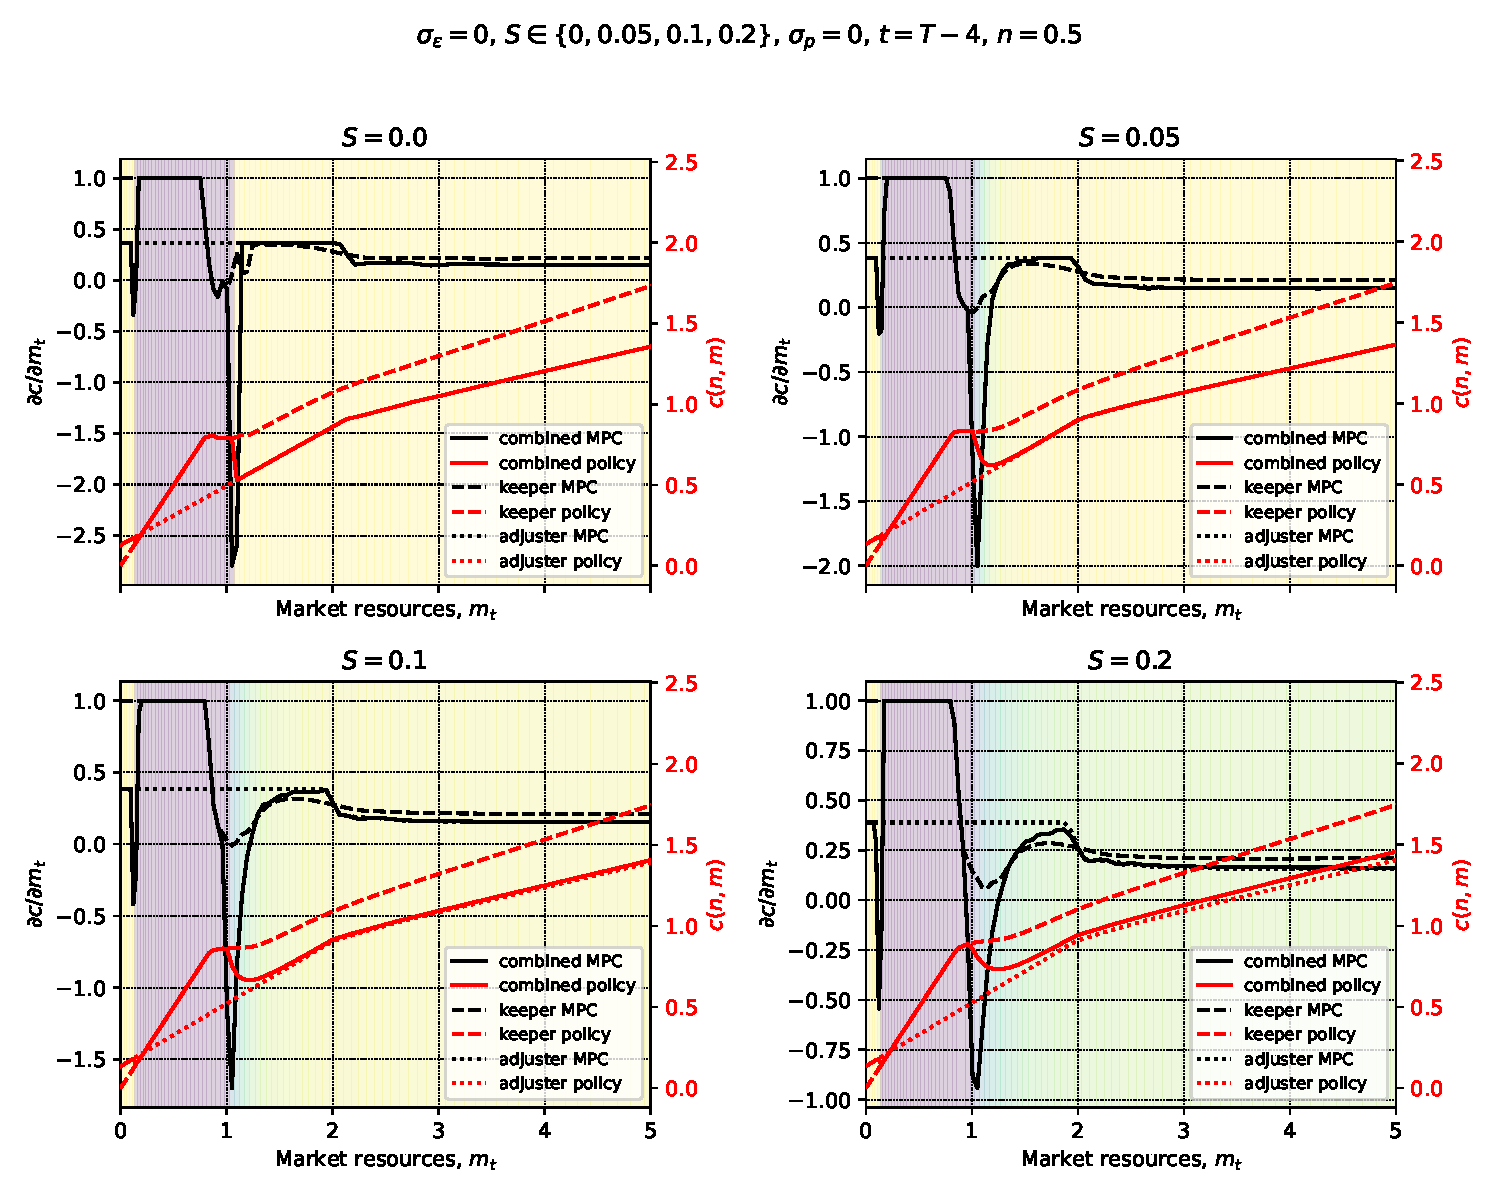
\includegraphics[width=\linewidth]{../../Figures/DurableModel/Search_c_periodt_MPC_decomp.pdf}
		\caption{MPC decomposition of nondurable consumption $c_t(n_t,m_t)$.}
		\label{fig:search_c_periodt_MPC_decomp}
	\end{subfigure}
	\hfill
	\begin{subfigure}{0.48\textwidth}
		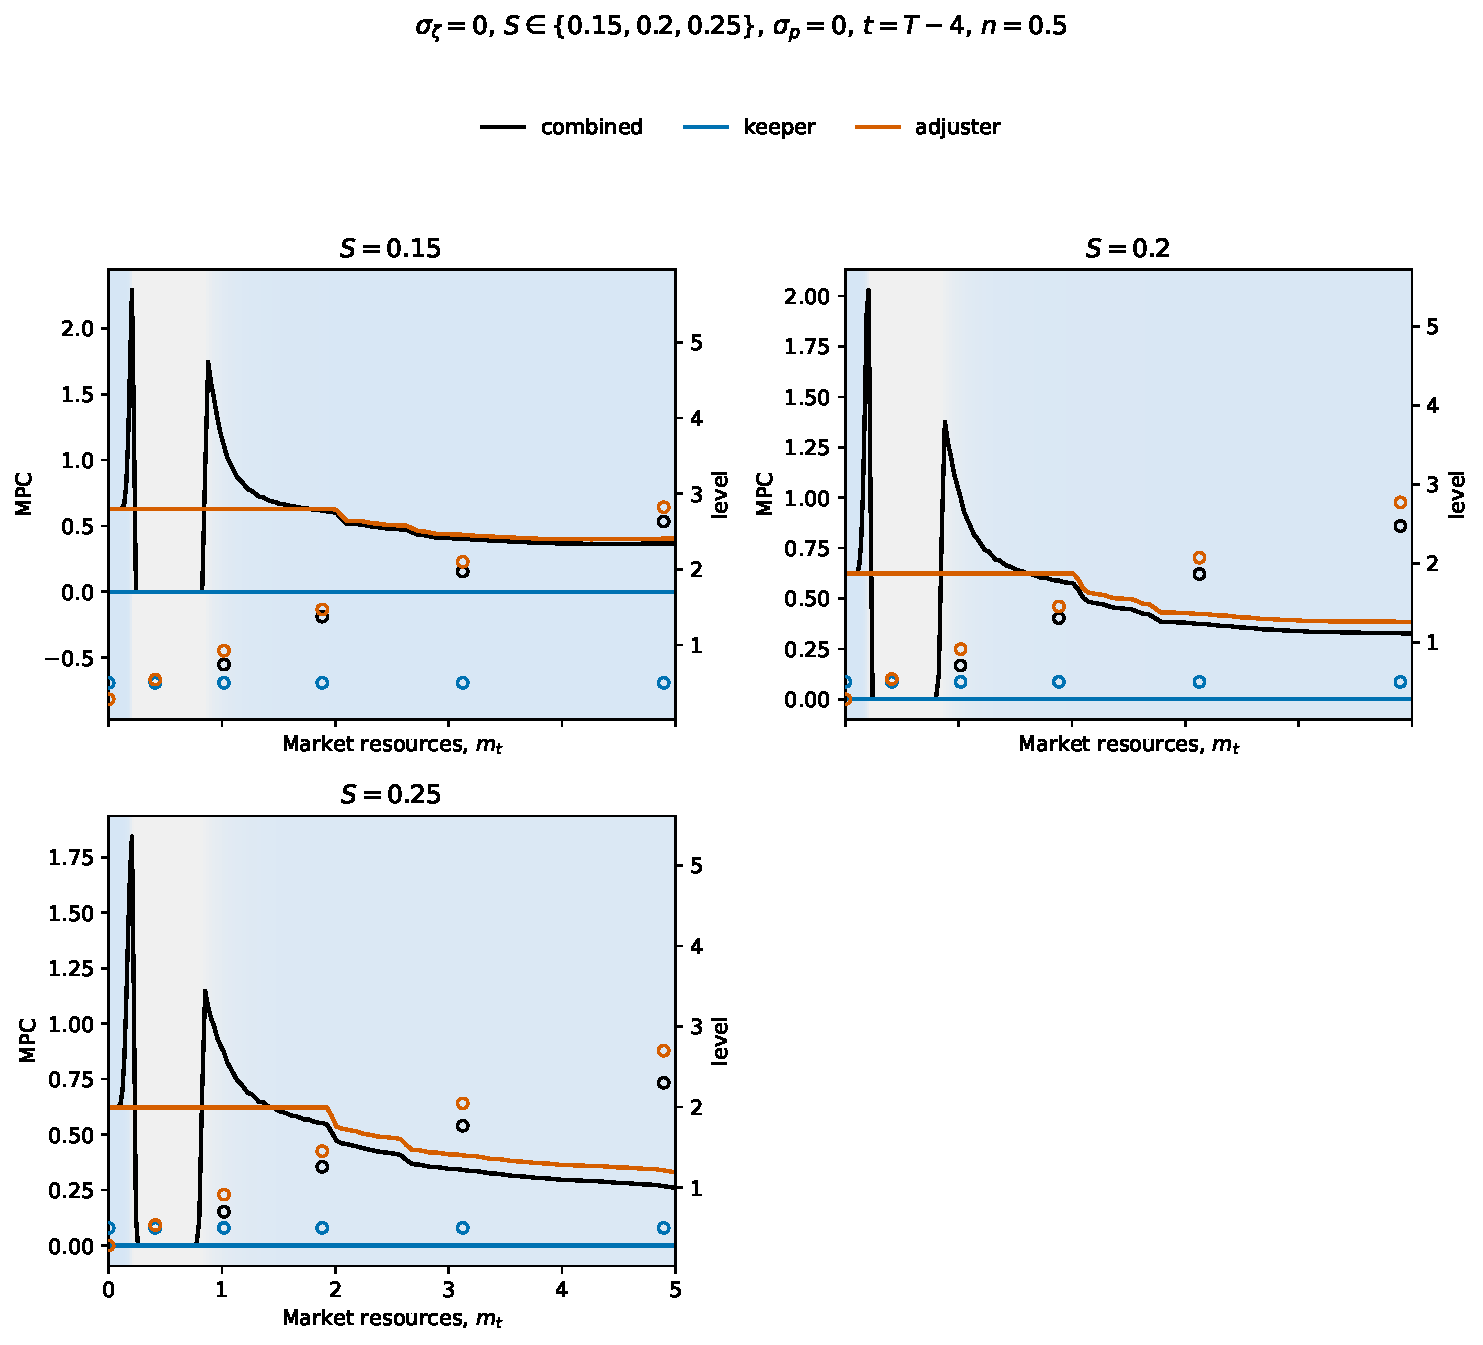
\includegraphics[width=\linewidth]{../../Figures/DurableModel/Search_d_periodt_MPC_decomp.pdf}
		\caption{MPC decomposition of durable consumption $d_t(n_t,m_t)$.}
		\label{fig:search_d_periodt_MPC_decomp}
	\end{subfigure}
	\caption{MPC and policy functions of non-durable and durable consumption using endogeneous search.}
	\label{fig:search_periodt_MPC_decomp}
\end{figure}


\subsection{Extension: Stochastic Durable Prices}\label{subsec:ModelBasicPrice}

This subsection introduces a third source of variation, orthogonal to the taste shocks of Section~\ref{subsec:ModelBasicTaste} and the search frictions of Section~\ref{subsec:ModelBasicSearch}: an idiosyncratic, i.i.d.\ shock to the relative price at which the durable good can be purchased in the period of adjustment. Neither taste shocks nor search frictions are present in this subsection, so the discrete choice between keeping and adjusting again resolves through a hard maximum, but now the adjuster's problem---and hence the comparison itself---is contingent on the realized price.

At the start of period $t$, after the transitory income shock $\theta_t$ has materialized, the household observes an i.i.d.\ relative price $p_t$ at which new units of the durable good can be bought this period. The price is log-normally distributed with mean one,
\begin{align}
	\log p_t \sim \mathcal{N}\Big(-\frac{\sigma_p^2}{2},\, \sigma_p^2\Big), \qquad \mathbb{E}[p_t] = 1, \label{eq:price_dist}
\end{align}
independent of $\theta_t$ and independent across periods. Only the \emph{purchase} of new durables is exposed to this price risk: households liquidate their existing durable stock exactly as in the baseline model, at the fixed proportional recovery rate $1-\tau$, so the liquidity available upon adjustment, $\ell_t = m_t + (1-\tau)n_t$, is unaffected by $p_t$. This is consistent with an interpretation in which trading in a used durable is governed by a separate, deterministic adjustment cost, while the price of a new unit on the market this period fluctuates, e.g.\ a household trading in a used car against the fluctuating price of a new one.

The keeper's problem is entirely unaffected by $p_t$, since no purchase occurs, so $v_t^{\text{keep}}(m_t,n_t)$ retains its baseline Bellman definition. The adjuster's budget constraint, however, now reads
\begin{align}
	a_t = \ell_t - c_t - p_t\, d_t \ge 0, \label{eq:price_budget}
\end{align}
in place of $a_t=\ell_t-c_t-d_t$, so the conditional value function becomes a function of both $\ell_t$ and $p_t$,
\begin{align}
	v_t^{\text{adj}}(\ell_t,p_t) &= \max_{c_t,d_t} \ u(c_t,d_t) + \beta \mathbb{E}_t \big[ v_{t+1}(m_{t+1},n_{t+1}) \big],\\
	& \text{s.t. equation~\eqref{eq:price_budget},}\\
	& \qquad m_{t+1} = \mathcal{R} a_t + \theta_{t+1}, \qquad n_{t+1} = (1-\delta)\,d_t.
\end{align}
Everything else about the household's environment---the interest rate $\mathcal{R}$, the depreciation rate $\delta$, and the no-borrowing constraint $a_t \ge 0$---is unchanged, and next period's durable stock $n_{t+1}$ continues to be measured in physical units, so $p_t$ affects only the current-period cost of acquiring $d_t$, not its future service flow beyond ordinary depreciation.

With the price-contingent budget constraint~\eqref{eq:price_budget}, the adjuster's Lagrangian is
\begin{align}
	\mathscr{L} = u(c_t,d_t) + \beta \mathbb{E}_t\big[v_{t+1}(m_{t+1},n_{t+1})\big] + \lambda_t^{\mathrm{adj}}\big(\ell_t - c_t - p_t\, d_t - a_t\big),
\end{align}
with $m_{t+1}=\mathcal{R}a_t+\theta_{t+1}$ and $n_{t+1}=(1-\delta)d_t$. The first-order conditions with respect to $c_t$, $a_t$, and $d_t$ are
\begin{align}
	\frac{\partial \mathscr{L}}{\partial c_t} &= u_c(c_t,d_t) - \lambda_t^{\mathrm{adj}} = 0
	&&\Longrightarrow\quad \lambda_t^{\mathrm{adj}} = u_c(c_t,d_t), \label{eq:price_foc_c}\\
	\frac{\partial \mathscr{L}}{\partial a_t} &= \beta \mathcal{R}\, \mathbb{E}_t\big[v_{t+1}^m\big] - \lambda_t^{\mathrm{adj}} = 0
	&&\Longrightarrow\quad \lambda_t^{\mathrm{adj}} = \beta \mathcal{R}\, \mathbb{E}_t\big[v_{t+1}^m\big], \label{eq:price_foc_a}\\
	\frac{\partial \mathscr{L}}{\partial d_t} &= u_d(c_t,d_t) + \beta(1-\delta)\,\mathbb{E}_t\big[v_{t+1}^n\big] - p_t\,\lambda_t^{\mathrm{adj}} = 0
	&&\Longrightarrow\quad u_d(c_t,d_t) = p_t\,\lambda_t^{\mathrm{adj}} - \beta(1-\delta)\,\mathbb{E}_t\big[v_{t+1}^n\big]. \label{eq:price_foc_d}
\end{align}
In KKT form, these are the price-modified analogues of the baseline conditions~\eqref{eq:FOC_c_basic}--\eqref{eq:FOC_d_basic}:
\begin{align}
	u_c(c_t, d_t) &\geq \beta \mathcal{R}\, \mathbb{E}_t \big[v_{t+1}^m\big], \\
	u_d(c_t, d_t) &\geq p_t\,\beta \mathcal{R}\, \mathbb{E}_t\big[v_{t+1}^m\big] - \beta (1 - \delta)\, \mathbb{E}_t\big[v_{t+1}^n\big].
\end{align}
Equation~\eqref{eq:price_foc_c} is identical in form to~\eqref{eq:FOC_c_basic}: because $p_t$ multiplies only $d_t$ in the budget, it does not appear in the $c_t$ first-order condition, so $c_t^{\mathrm{adj},\ast}$ solves the same equation as in the baseline model \emph{given} $d_t$. Equation~\eqref{eq:price_foc_d} differs from~\eqref{eq:FOC_d_basic}: the marginal cost of an extra unit of durables is now $p_t\lambda_t^{\mathrm{adj}}$ rather than $\lambda_t^{\mathrm{adj}}$, since each unit of $d_t$ costs $p_t$ units of $\ell_t$ instead of one. Equality holds when the borrowing constraint does not bind.

Because $p_t$ is observed before the discrete choice is made, the household's beginning-of-period problem is the price-contingent hard maximum
\begin{align}
	v_t(m_t,n_t,p_t) = \max\Big\{ v_t^{\text{keep}}(m_t,n_t),\; v_t^{\text{adj}}(\ell_t,p_t)\Big\}. \label{eq:price_discrete}
\end{align}
A high realization of $p_t$ raises the marginal cost of adjusting and, other things equal, makes the household less likely to adjust and, conditional on adjusting, to purchase a smaller quantity of the durable; a low realization has the opposite effect. Because agents can reject an offer when the drawn price leads to an allocation which is worse than the keeper solution, the model induces state-contingent variation in both the adjustment margin and the size of the resulting durable purchase.

As with the EV Type I inclusive value, the object that matters for the previous period's continuation value is the price-integrated value function
\begin{align}
	\bar v_t(m_t,n_t) \equiv \mathbb{E}_{p_t}\Big[v_t(m_t,n_t,p_t)\Big]
	= \mathbb{E}_{p_t}\Big[\max\big\{ v_t^{\text{keep}}(m_t,n_t),\; v_t^{\text{adj}}(\ell_t,p_t) \big\}\Big], \label{eq:price_barv}
\end{align}
which replaces $v_t(m_t,n_t)$ inside the Bellman equations for $v_{t-1}^{\text{keep}}$ and $v_{t-1}^{\text{adj}}$. Unlike EV Type I taste shocks, which leave the adjuster's optimal continuous choices unchanged and only reweight the discrete comparison through logit probabilities, the price shock changes the adjuster's optimal consumption-durable split itself, so $v_t^{\text{adj}}(\ell_t,p_t)$ must be solved separately for every relevant realization of $p_t$; the resulting policy functions $c_t^{\text{adj}}(\ell_t,p_t)$ and $d_t^{\text{adj}}(\ell_t,p_t)$ are likewise price-contingent, and the model's reported (ex-ante) nondurable-consumption and durable-purchase functions are price-weighted averages of these state-contingent choices, in the same spirit as $\bar v_t$. As $\sigma_p \to 0$, $p_t \to 1$ almost surely and the model collapses to the hard-maximum baseline of Section~\ref{sec:ModelBasic}. I derive the envelope conditions, the terminal-period solution, and the EGM algorithm with stochastic durable prices in appendix~\ref{subsec:appdx_price_basic}.

Even stochastic prices induce enough uncertainty to lead to adjusting intensities between zero and one as seen in
fig~\ref{fig:pricestd_Ss_T}. However, since sharp thresholds still exist, the consumption functions in T-1 are not as smooth as with taste shocks or endogeneous search.

\begin{figure}[htbp]
	\centering
	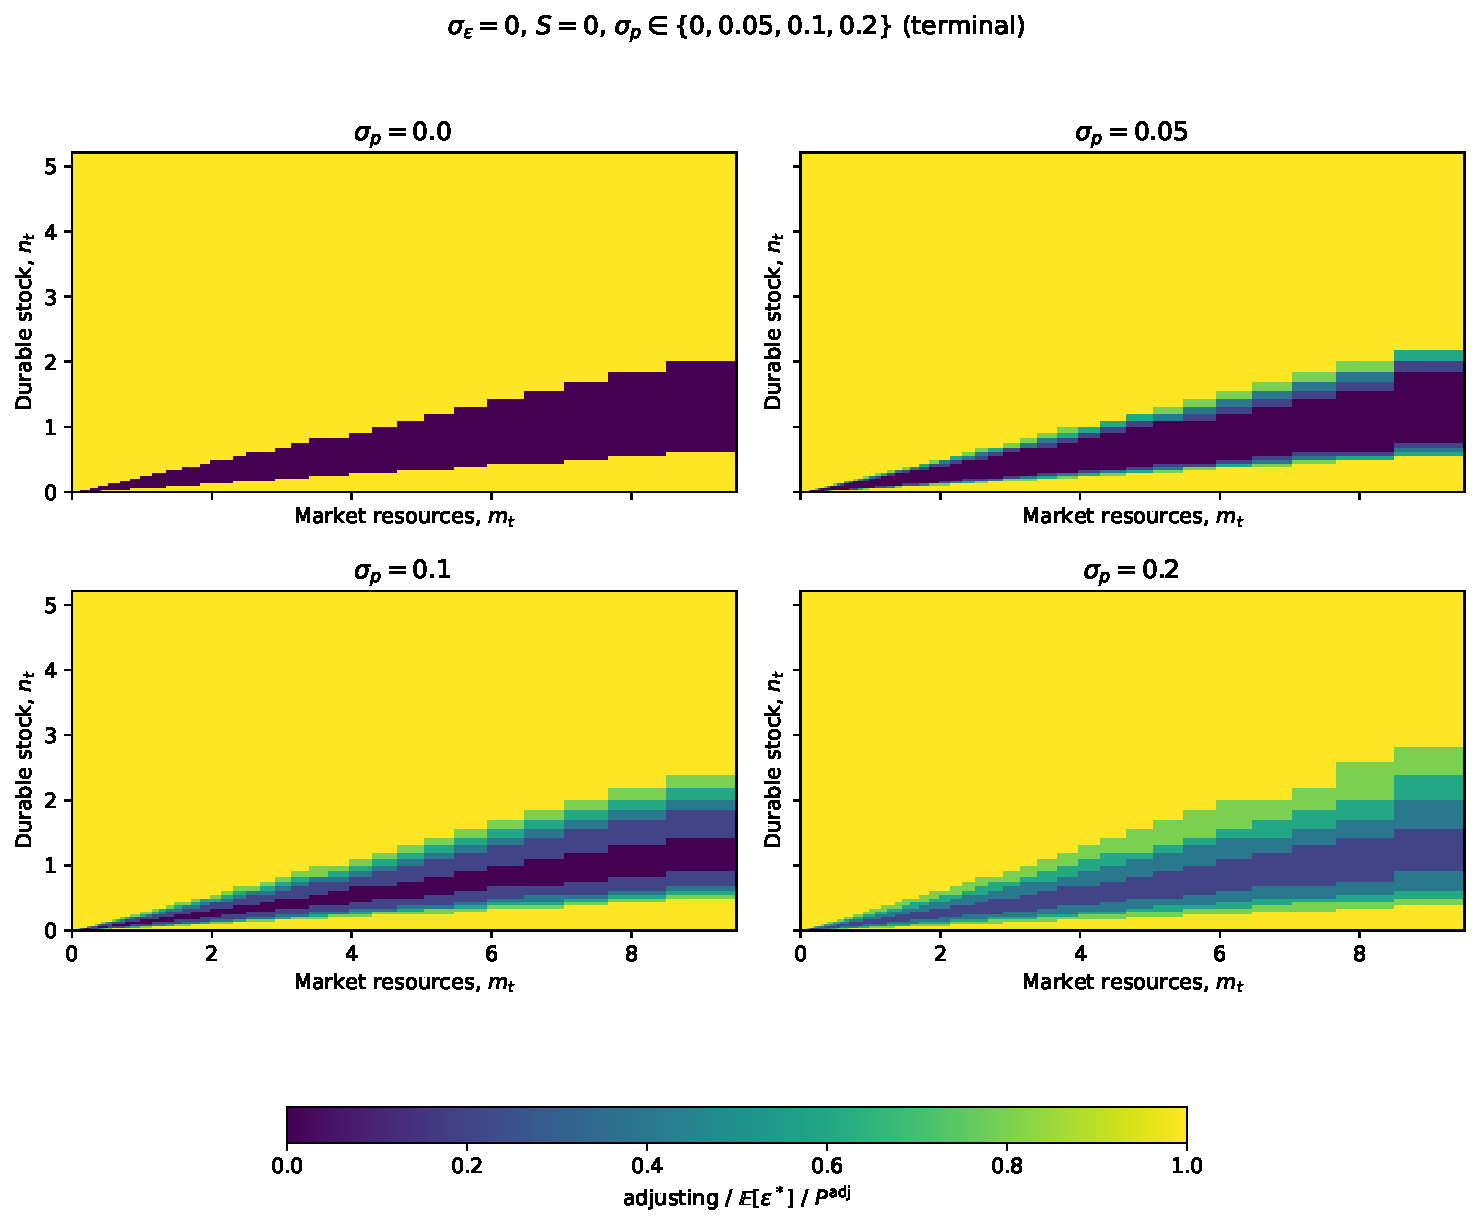
\includegraphics[width=0.85\linewidth]{../../Figures/DurableModel/PriceStd_Ss_T.pdf}
	\caption{Adjustment regions in period $T$ under stochastic durable prices for $\sigma_p \in \{0, 0.05, 0.1, 0.2\}$ (fixed number of price nodes). Greater price dispersion softens the hard keep--adjust threshold.}
	\label{fig:pricestd_Ss_T}
\end{figure}

Figure~\ref{fig:PriceStd_periodt_MPC_decomp} shows the policy functions for variation in the price dispersion and figure~\ref{fig:PriceCount_periodt_MPC_decomp} for a coraser grid of price points.

\begin{figure}[htbp]
	\centering
	\begin{subfigure}{0.48\textwidth}
		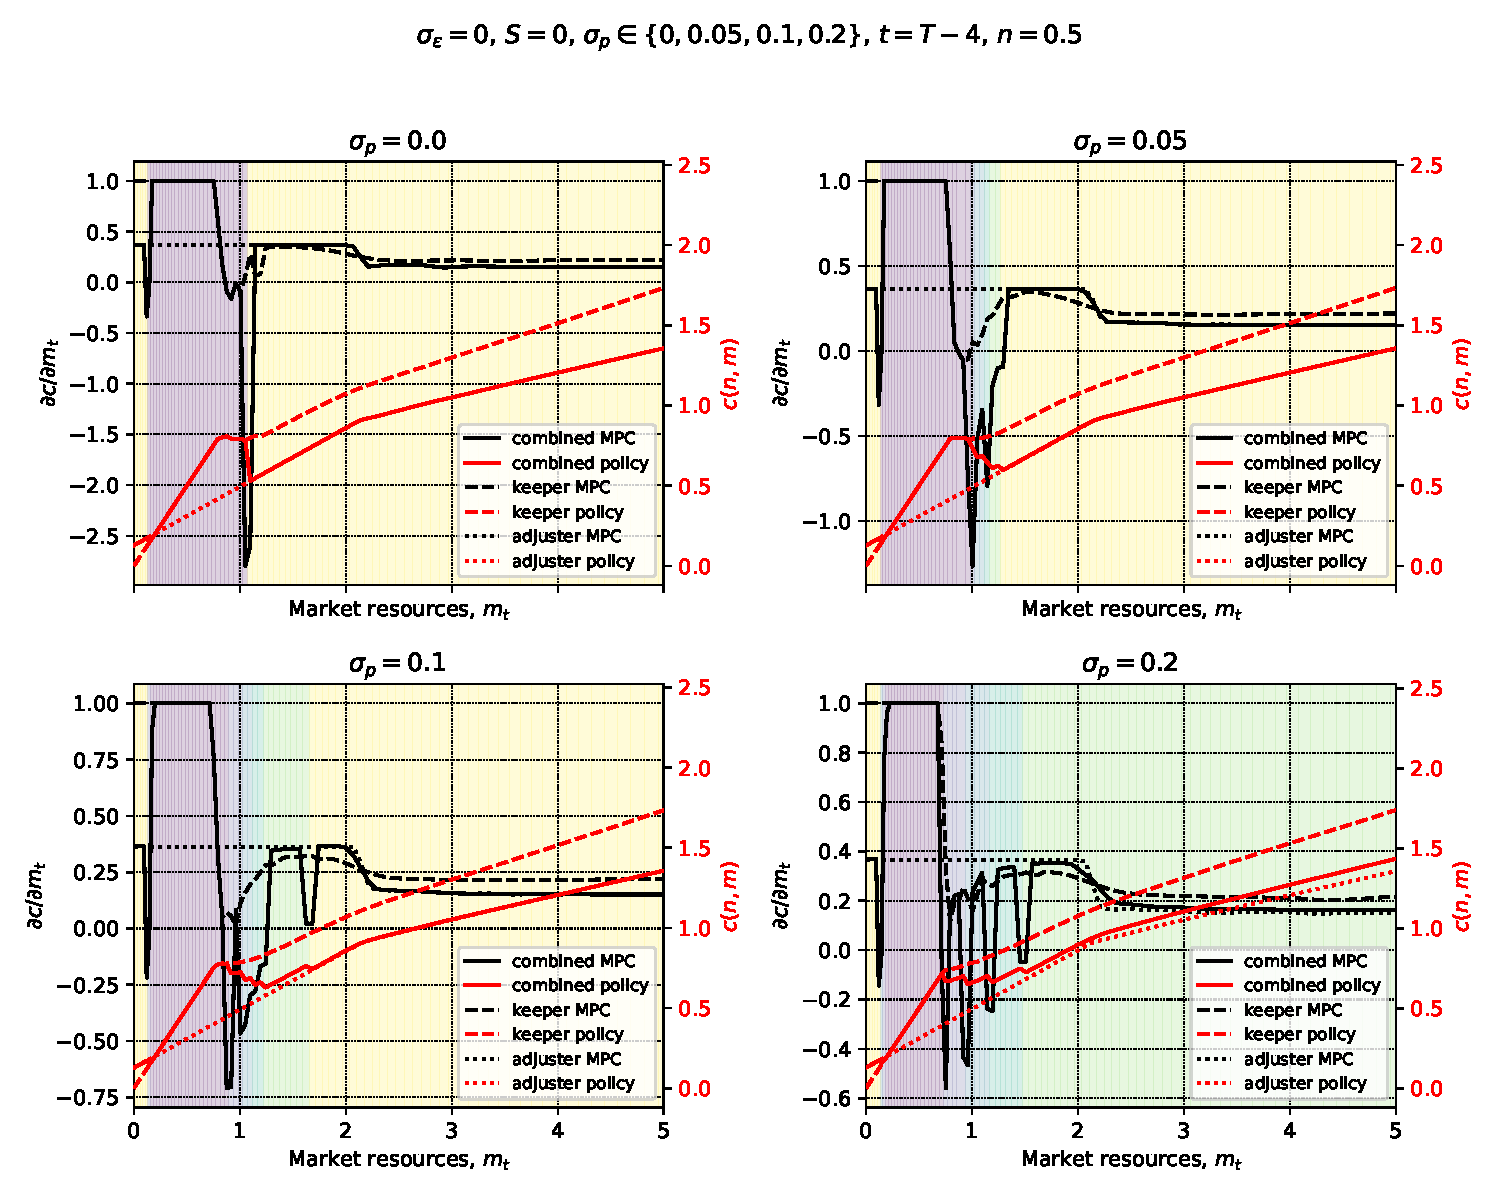
\includegraphics[width=\linewidth]{../../Figures/DurableModel/PriceStd_c_periodt_MPC_decomp.pdf}
		\caption{MPC decomposition of nondurable consumption $c_t(n_t,m_t)$.}
		\label{fig:PriceStd_c_periodt_MPC_decomp}
	\end{subfigure}
	\hfill
	\begin{subfigure}{0.48\textwidth}
		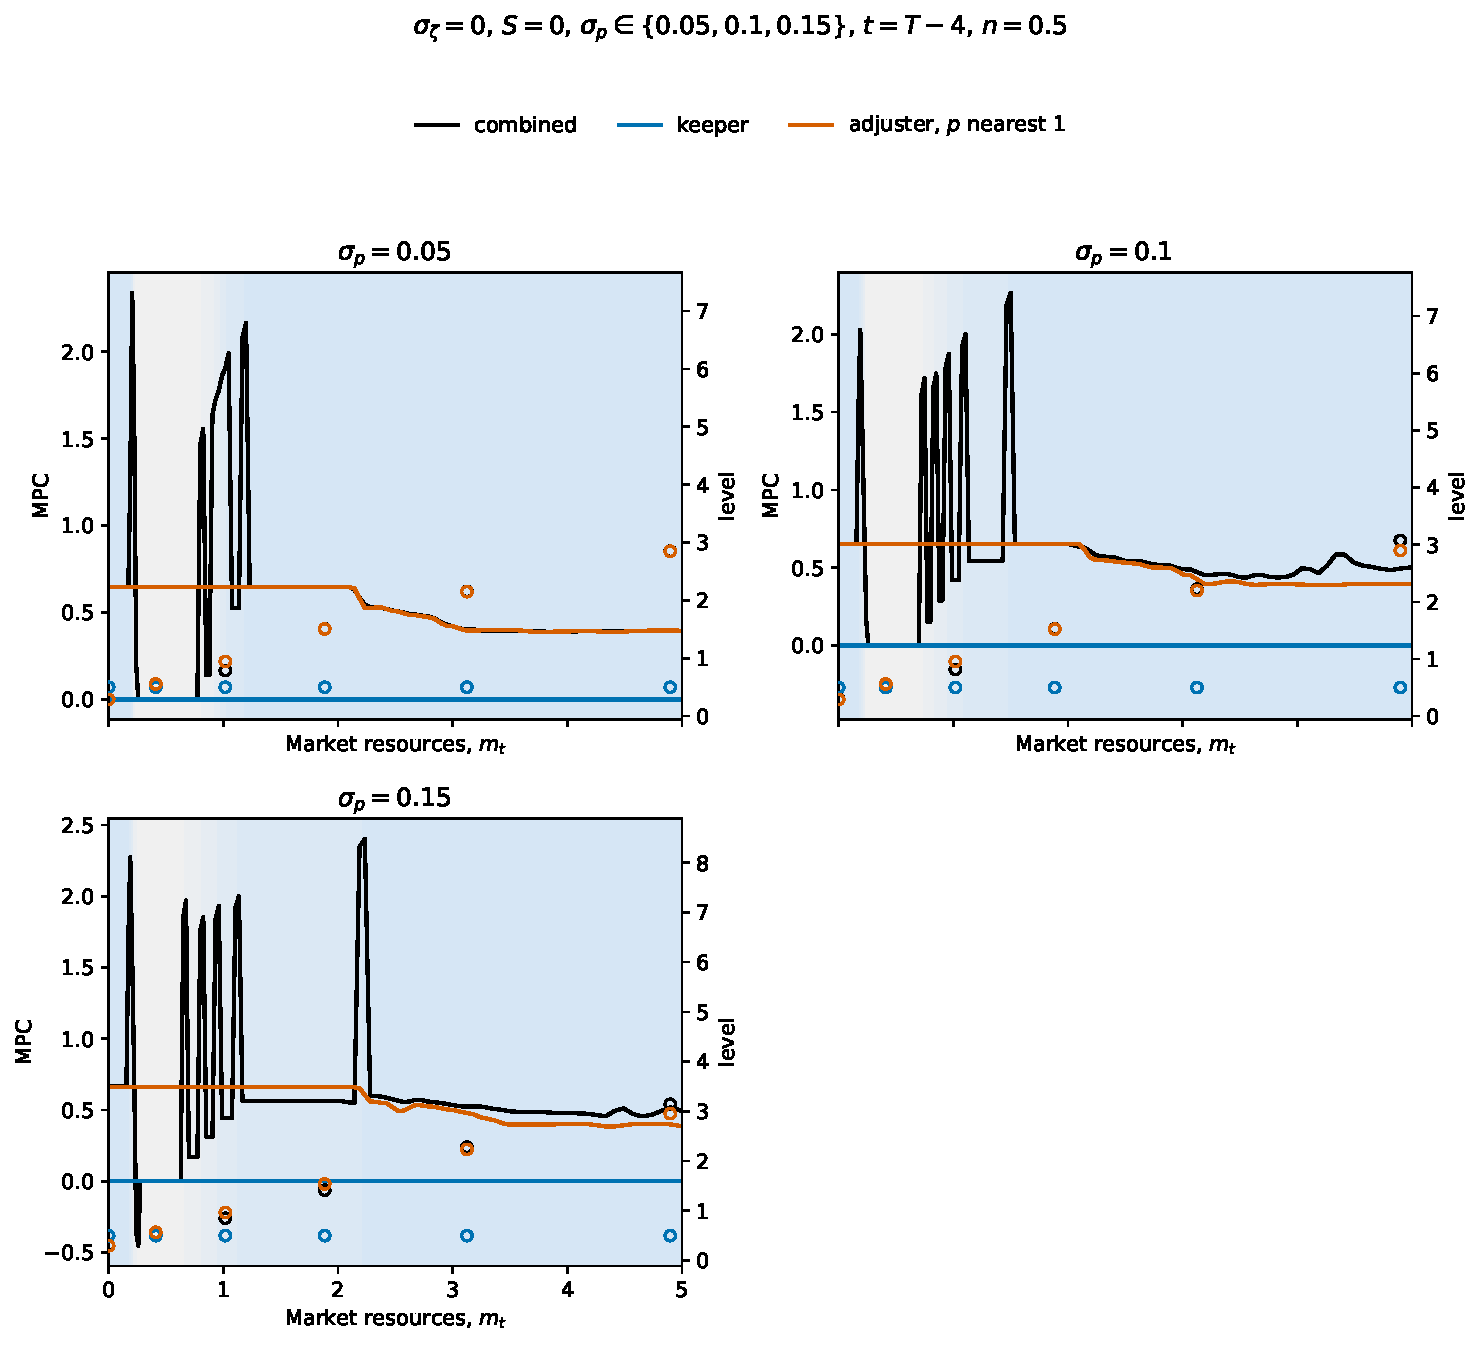
\includegraphics[width=\linewidth]{../../Figures/DurableModel/PriceStd_d_periodt_MPC_decomp.pdf}
		\caption{MPC decomposition of durable consumption $d_t(n_t,m_t)$.}
		\label{fig:PriceStd_d_periodt_MPC_decomp}
	\end{subfigure}
	\caption{MPC and policy functions of non-durable and durable consumption using stochastic prices.}
	\label{fig:PriceStd_periodt_MPC_decomp}
\end{figure}


\begin{figure}[htbp]
	\centering
	\begin{subfigure}{0.48\textwidth}
		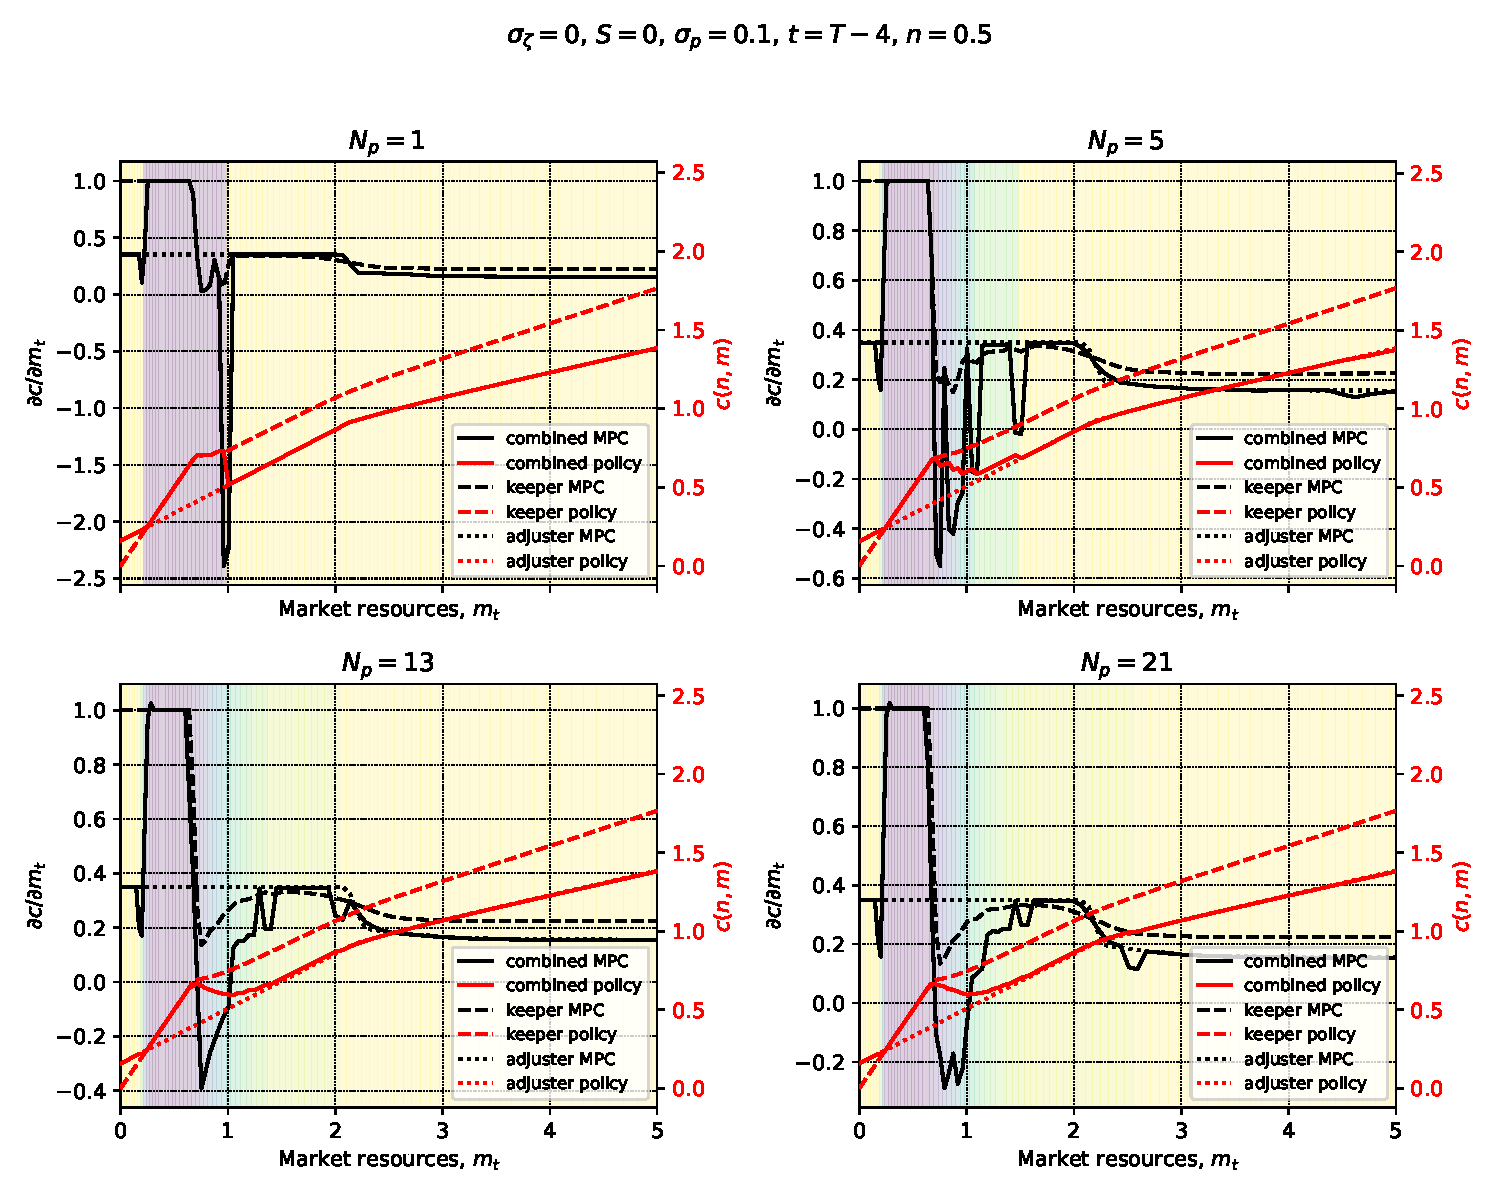
\includegraphics[width=\linewidth]{../../Figures/DurableModel/PriceCount_c_periodt_MPC_decomp.pdf}
		\caption{MPC decomposition of nondurable consumption $c_t(n_t,m_t)$.}
		\label{fig:PriceCount_c_periodt_MPC_decomp}
	\end{subfigure}
	\hfill
	\begin{subfigure}{0.48\textwidth}
		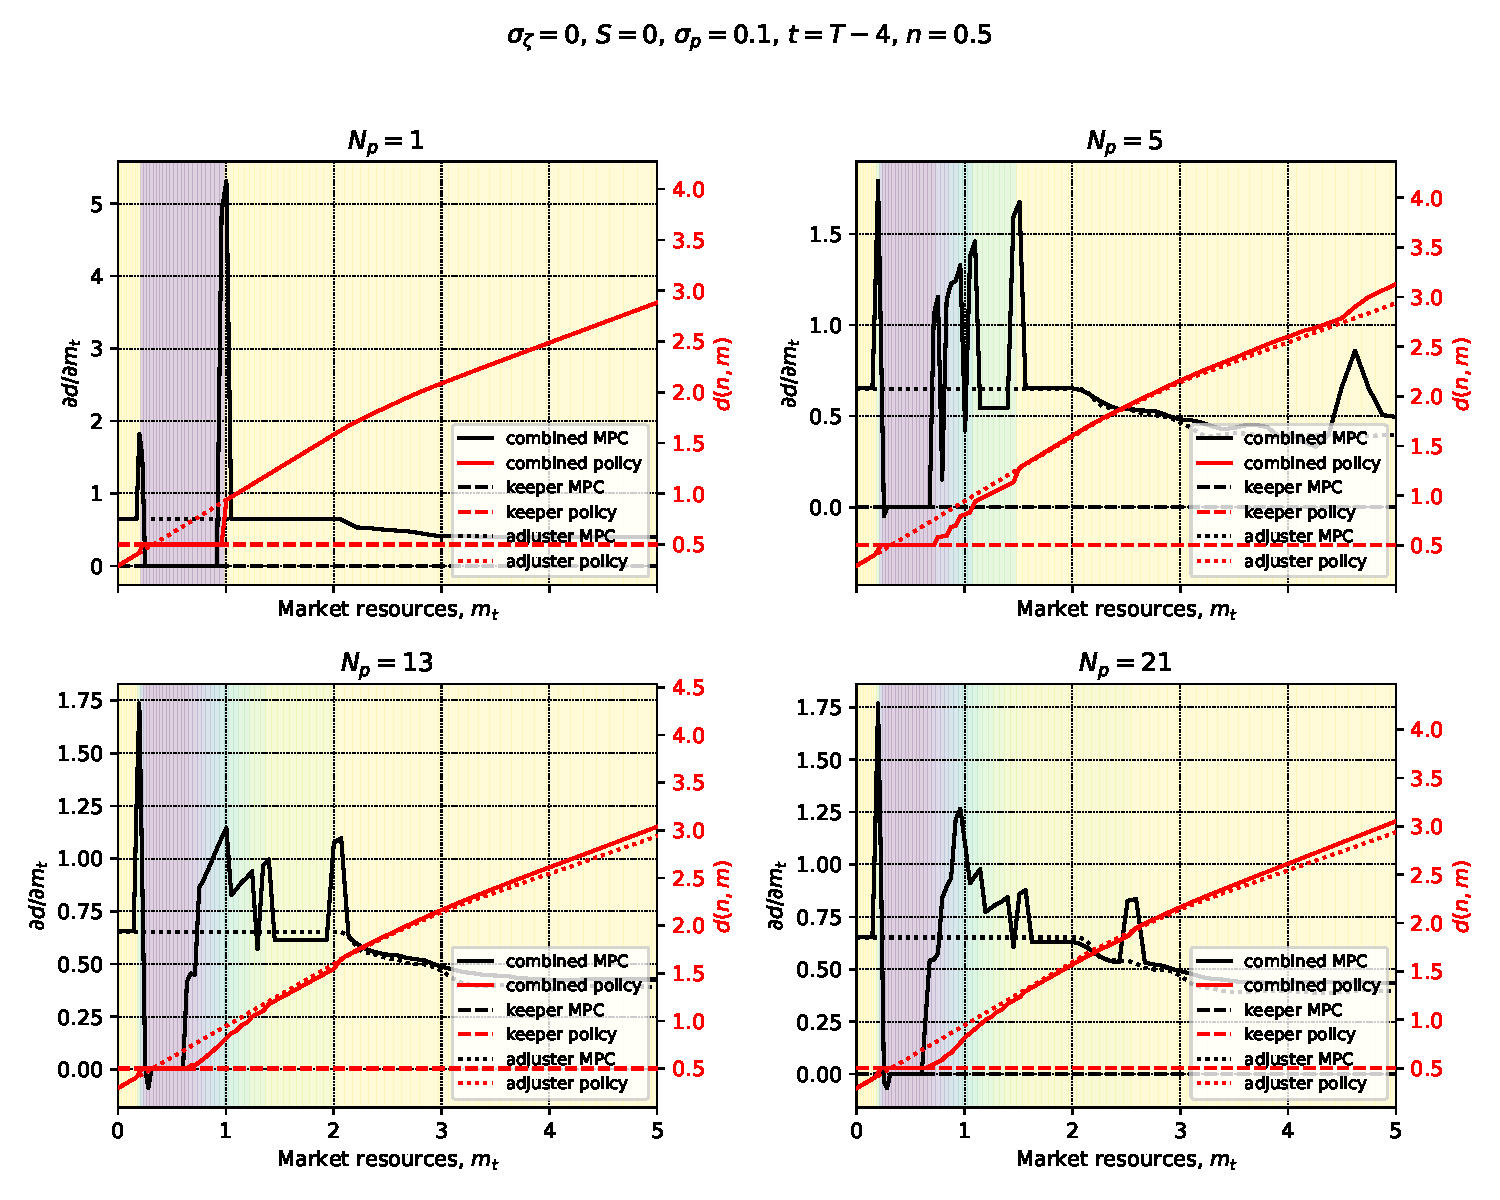
\includegraphics[width=\linewidth]{../../Figures/DurableModel/PriceCount_d_periodt_MPC_decomp.pdf}
		\caption{MPC decomposition of durable consumption $d_t(n_t,m_t)$.}
		\label{fig:PriceCount_d_periodt_MPC_decomp}
	\end{subfigure}
	\caption{MPC and policy functions of non-durable and durable consumption varying the number of price points.}
	\label{fig:PriceCount_periodt_MPC_decomp}
\end{figure}


\subsection{Extension: Search and Stochastic Prices}\label{subsec:ModelBasicFull}

This subsection nests the search frictions of Section~\ref{subsec:ModelBasicSearch} with the stochastic durable prices of Section~\ref{subsec:ModelBasicPrice}. Extreme Value Type I taste shocks (Section~\ref{subsec:ModelBasicTaste}) and directed search are alternative ways of smoothing the keep-versus-adjust margin; nesting both would double-smooth the discrete choice without a clear economic interpretation, so the nested environment uses search rather than EV Type I shocks, together with price risk on the adjuster's continuous problem.

The household faces an idiosyncratic relative price $p_t$ at which new durables can be purchased and chooses a search intensity $\varepsilon_t\in[0,1]$ that determines the probability of successfully adjusting, at convex cost $\sigma(\varepsilon_t)$ from equation~\eqref{eq:search_cost_basic}. The price is independent of income,
\begin{align}
	\log p_t &\sim \mathcal{N}\Big(-\frac{\sigma_p^2}{2},\,\sigma_p^2\Big), \qquad \mathbb{E}[p_t]=1, \label{eq:full_p_dist}
\end{align}
with $p_t\perp\theta_t$ and i.i.d.\ across periods.

The within-period timeline is as follows. After $\theta_t$ has materialized and $(m_t,n_t)$ are known, the household observes $p_t$. Liquidity upon adjustment remains $\ell_t=m_t+(1-\tau)n_t$, independent of the price. The keeper's problem is unaffected by $p_t$, so $v_t^{\text{keep}}(m_t,n_t)$ retains its baseline Bellman definition. The adjuster's budget constraint is the price-contingent constraint~\eqref{eq:price_budget}, so the adjuster's conditional value $v_t^{\text{adj}}(\ell_t,p_t)$ and its continuous policies $c_t^{\text{adj}}(\ell_t,p_t)$, $d_t^{\text{adj}}(\ell_t,p_t)$ are exactly as in Section~\ref{subsec:ModelBasicPrice}. Given these two conditional values, the household chooses search intensity to maximize the price-contingent objective
\begin{align}
	v_t(m_t,n_t,p_t)
	&= \max_{\varepsilon_t\in[0,1]}
	\Big[(1-\varepsilon_t)\, v_t^{\text{keep}}(m_t,n_t)
	+ \varepsilon_t\, v_t^{\text{adj}}(\ell_t,p_t)
	- \sigma(\varepsilon_t)\Big]. \label{eq:full_discrete}
\end{align}
Equation~\eqref{eq:full_discrete} nests the standalone search and price extensions as special cases: with $\sigma_p\to 0$ it collapses to the search problem~\eqref{eq:search_discrete_basic}; with $S\to 0$ it collapses to the price-contingent hard maximum~\eqref{eq:price_discrete}; and with both limits simultaneous it collapses to the hard-maximum baseline of Section~\ref{sec:ModelBasic}.

Because $p_{t+1}$ is drawn afresh every period, the object that enters today's Euler equations is the price-integrated value function
\begin{align}
	\bar v_t(m_t,n_t)
	&\equiv \mathbb{E}_{p_t}\big[v_t(m_t,n_t,p_t)\big], \label{eq:full_barv}
\end{align}
which replaces $v_t(m_t,n_t)$ inside the Bellman equations for $v_{t-1}^{\text{keep}}$ and $v_{t-1}^{\text{adj}}$. The two frictions play complementary roles: $p_t$ shifts the adjuster's continuous problem and therefore the level of $v_t^{\text{adj}}$; and $\varepsilon_t^\ast$ translates the resulting gap $v_t^{\text{adj}}-v_t^{\text{keep}}$ into a smooth probability of adjusting. I derive the optimal search-effort rule, the combined envelope conditions, the Euler equations, the terminal-period solution, and the EGM algorithm for the nested model in appendix~\ref{subsec:appdx_full_basic}.

Using a combination of endogeneous search and stochastic prices can smooth policy functions when searchfrictions are not enough. Figure~\ref{fig:pricestd_search_Ss_T} illustrates the S,s region for the terminal period, and figure~\ref{fig:PriceStd_Search_periodt_MPC_decomp} shows the MPCs in period t.


\begin{figure}[htbp]
	\centering
	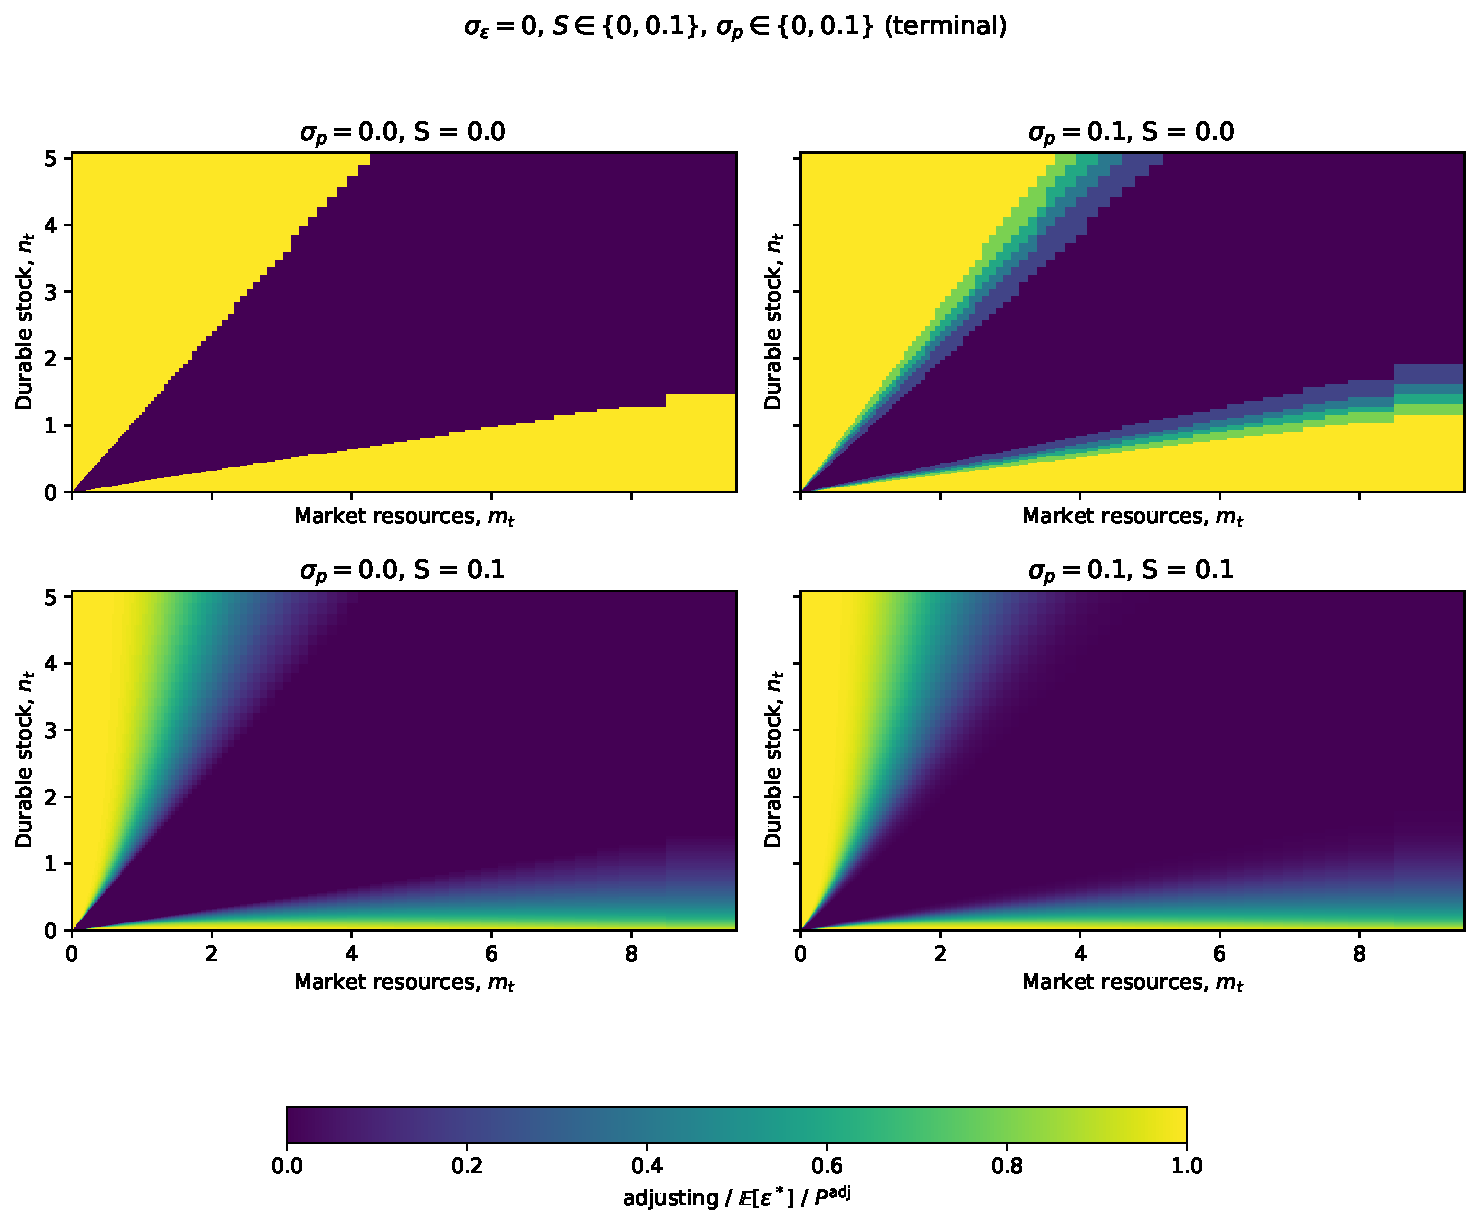
\includegraphics[width=0.85\linewidth]{../../Figures/DurableModel/PriceStd_Search_Ss_T.pdf}
	\caption{Adjustment regions in period $T$ under stochastic durable prices and endogeneous search.}
	\label{fig:pricestd_search_Ss_T}
\end{figure}


\begin{figure}[htbp]
	\centering
	\begin{subfigure}{0.48\textwidth}
		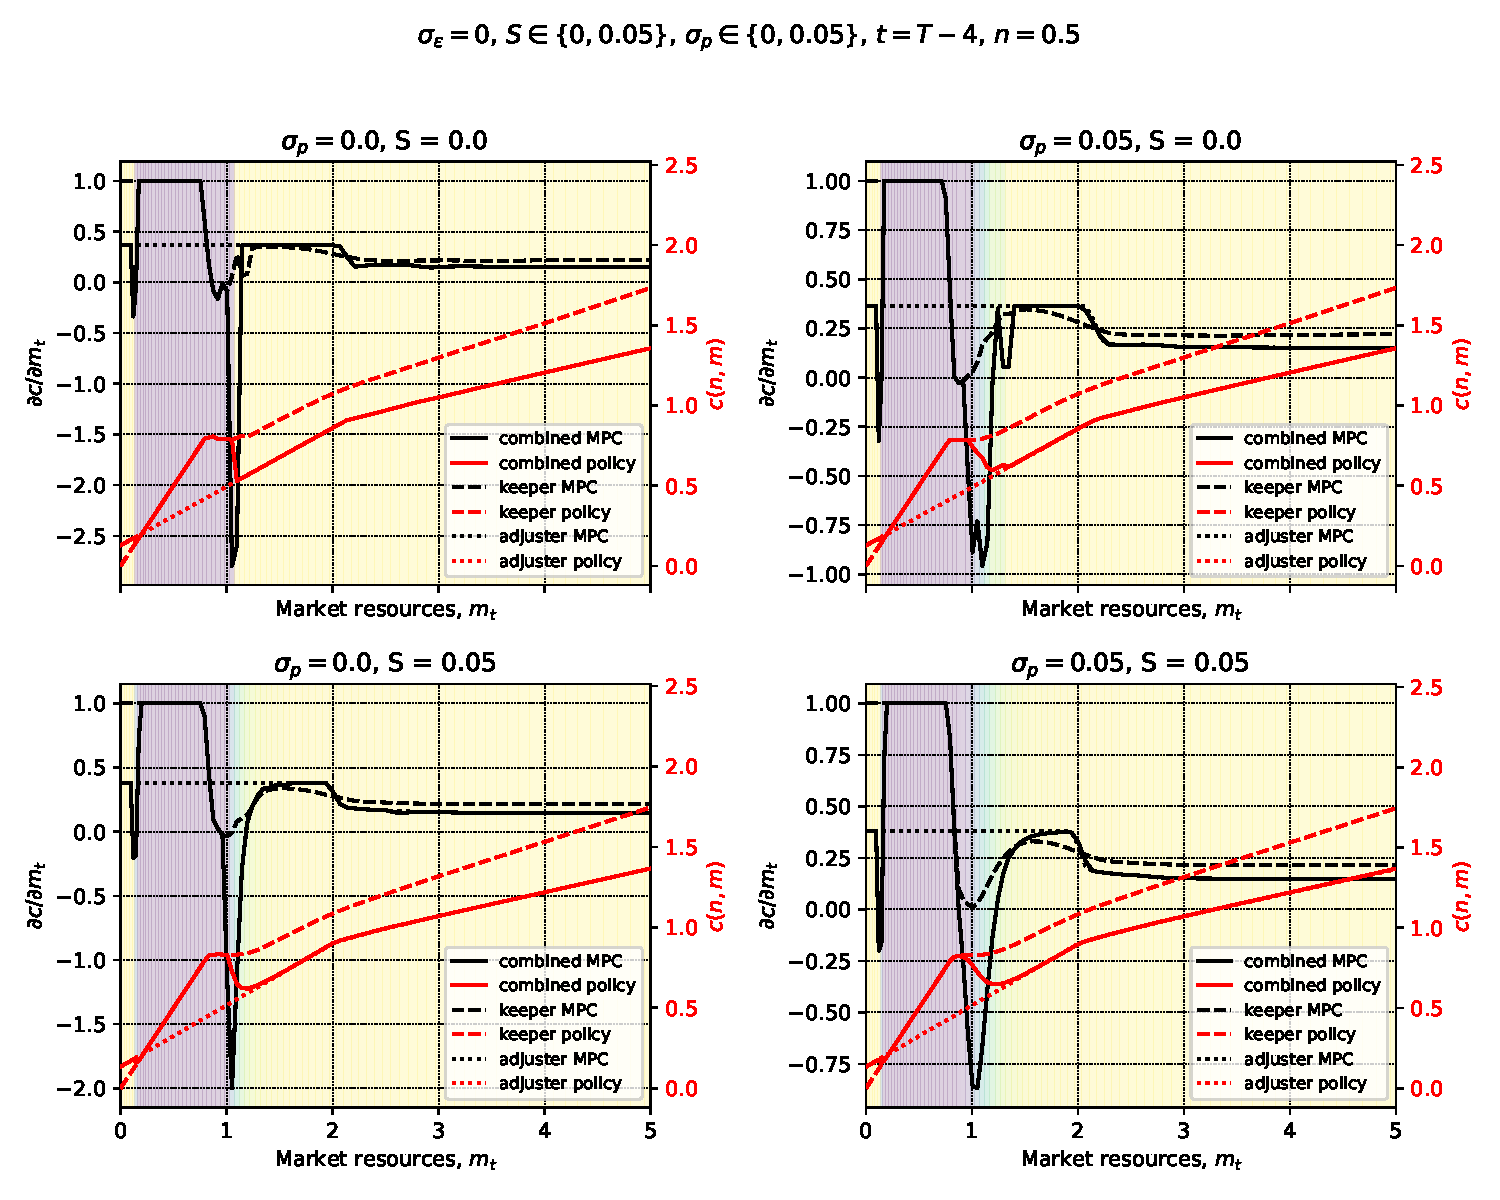
\includegraphics[width=\linewidth]{../../Figures/DurableModel/PriceStd_Search_c_periodt_MPC_decomp.pdf}
		\caption{MPC decomposition of nondurable consumption $c_t(n_t,m_t)$.}
		\label{fig:PriceStd_Search_c_periodt_MPC_decomp}
	\end{subfigure}
	\hfill
	\begin{subfigure}{0.48\textwidth}
		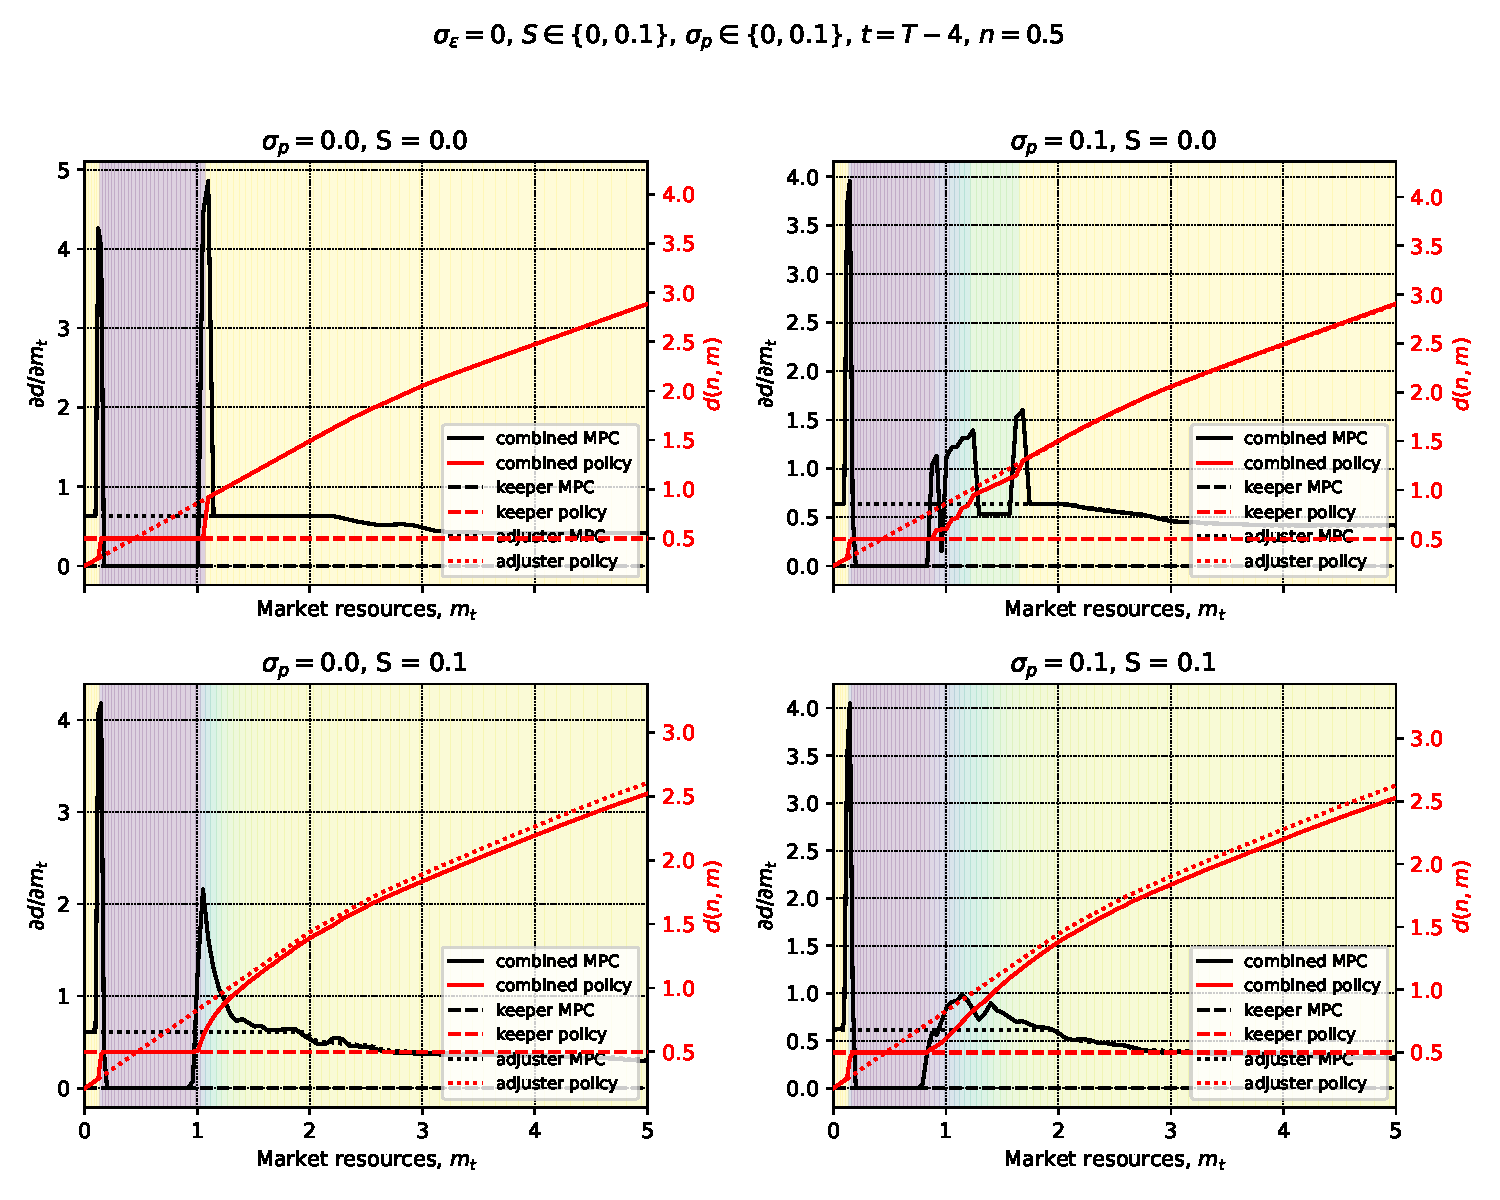
\includegraphics[width=\linewidth]{../../Figures/DurableModel/PriceStd_Search_d_periodt_MPC_decomp.pdf}
		\caption{MPC decomposition of durable consumption $d_t(n_t,m_t)$.}
		\label{fig:PriceStd_Search_d_periodt_MPC_decomp}
	\end{subfigure}
	\caption{MPC and policy functions of non-durable and durable consumption using stochastic prices and search.}
	\label{fig:PriceStd_Search_periodt_MPC_decomp}
\end{figure}


\subsection{Comparing smoothness mechanisms: Lifecycle}\label{subsec:ModelBasicSmoothingCompare}

As in the retirement application of Section~\ref{sec:RetirementModel}, each of the mechanisms above---EV Type~I taste shocks $\sigma_\varepsilon$, search frictions $S$, durable-price dispersion $\sigma_p$, and transitory income risk $\sigma_\eta$---can smooth the discontinuities that arise from the hard keep-versus-adjust margin. It is therefore natural to ask whether they also shift the combined decision rules in economically distinct directions, as taste shocks and search frictions do for the worker's consumption function.

To make the comparison transparent, I fix beginning-of-period durables at a representative stock $n_t=n_0$ and plot the \emph{combined} policies $c_t(n_0,m_t)$ and $d_t(n_0,m_t)$ in an earlier period, together with the corresponding marginal propensities $\partial c_t/\partial m_t$ and $\partial d_t/\partial m_t$. Starting from a lightly smoothed reference in each channel, I then increase one smoothness parameter at a time (holding the others at their inactive values, except that the income experiment retains a small EV scale so that the discrete margin remains smooth). Figures~\ref{fig:smoothing_shifts_levels} and~\ref{fig:smoothing_shifts_mpcs} summarize the results.

In contrast to the retirement model, all four mechanisms move the durable policies in the \emph{same} direction. Raising $\sigma_\varepsilon$, $S$, $\sigma_p$, or $\sigma_\eta$ increases combined nondurable consumption, decreases combined durable holdings, and dampens the sharp MPC spikes that appear around the S,s band under a hard maximum. The common pattern reflects the nature of the discrete choice. Keep-versus-adjust reallocates a stock subject to a transaction cost $\tau$; it does not permanently alter the household's labor-income stream. Larger search costs, a more diffuse logit mix of keep and adjust, or greater ex-ante averaging over purchase prices all reduce the weight (or the extremity) of the full adjuster branch relative to keeping $d_t=n_t$. The combined rule therefore shifts toward the keeper---higher liquid consumption out of $m_t$ and a durable stock closer to the inherited $n_0$---and the discontinuous jump in MPCs at the S,s threshold is attenuated. Larger income shocks reinforce the same qualitative shift through standard precautionary saving into liquid resources.

These visual improvements are matched by the numerical kink diagnostics stored with each period's solution. For the keeper, I count decreasing segments of the EGM locus (the breaks between nondecreasing pieces that necessitate an upper envelope); for the adjuster, I count the FOC candidates removed by FUES. Table~\ref{tab:smoothing_kinks} reports both counts and shares in the same earlier period as Figures~\ref{fig:smoothing_shifts_levels}--\ref{fig:smoothing_shifts_mpcs}, for the hard-max baseline and one representative magnitude of each discrete-choice smoother. Relative to the hard maximum, taste shocks, search frictions, and price dispersion all drive the keeper's decreasing-segment count to zero. Taste shocks and search frictions also eliminate FUES removals in that period; price dispersion leaves a small residual share of removed adjuster points (the absolute count is not comparable to the single-price baseline because FUES is applied separately at each price node), but the keeper side is fully cleaned and the combined MPC spikes are still damped. A zero deletion count is not the same as an accurate interpolant; Section~\ref{subsec:ModelBasicEuler} pairs the counts with off-grid Euler residuals.

\begin{table}[htbp]
\centering
\caption{Period-$t$ kink diagnostics under the hard-max baseline and one smoothed magnitude of each discrete-choice channel. Keeper: number and share of decreasing EGM segments. Adjuster: number and share of FOC points removed by FUES. The $\sigma_p$ adjuster count sums over price nodes.}
\label{tab:smoothing_kinks}
\begin{tabular}{lcccc}
\hline
 & \multicolumn{2}{c}{Keeper} & \multicolumn{2}{c}{Adjuster} \\
\cline{2-3}\cline{4-5}
Specification & Decr.\ seg. & Share & Kinks rem. & Share \\
\hline
Hard max & 5 & 0.045 & 4 & 0.040 \\
$\sigma_\varepsilon = 0.05$ & 0 & 0 & 0 & 0 \\
$S = 0.1$ & 0 & 0 & 0 & 0 \\
$\sigma_p = 0.1$ & 0 & 0 & 17 & 0.035 \\
\hline
\end{tabular}
\end{table}

The retirement contrast is immediate. There, lowering the probability of a successful switch or raising search frictions reduces the likelihood of leaving work, so agents expect more years of labor income and consume more today; larger taste shocks instead raise the risk of retiring ``too early'' and induce precautionary saving, so consumption falls. Taste and search therefore shift the worker's rule in opposite directions even though both smooth the discrete margin. In the durable environment, both channels primarily reweight the same keep-versus-adjust comparison toward less aggressive adjustment, so their effects on combined $c_t$ and $d_t$ line up---as do price dispersion and income risk.

\begin{figure}[htbp]
	\centering
	\begin{subfigure}{0.48\textwidth}
		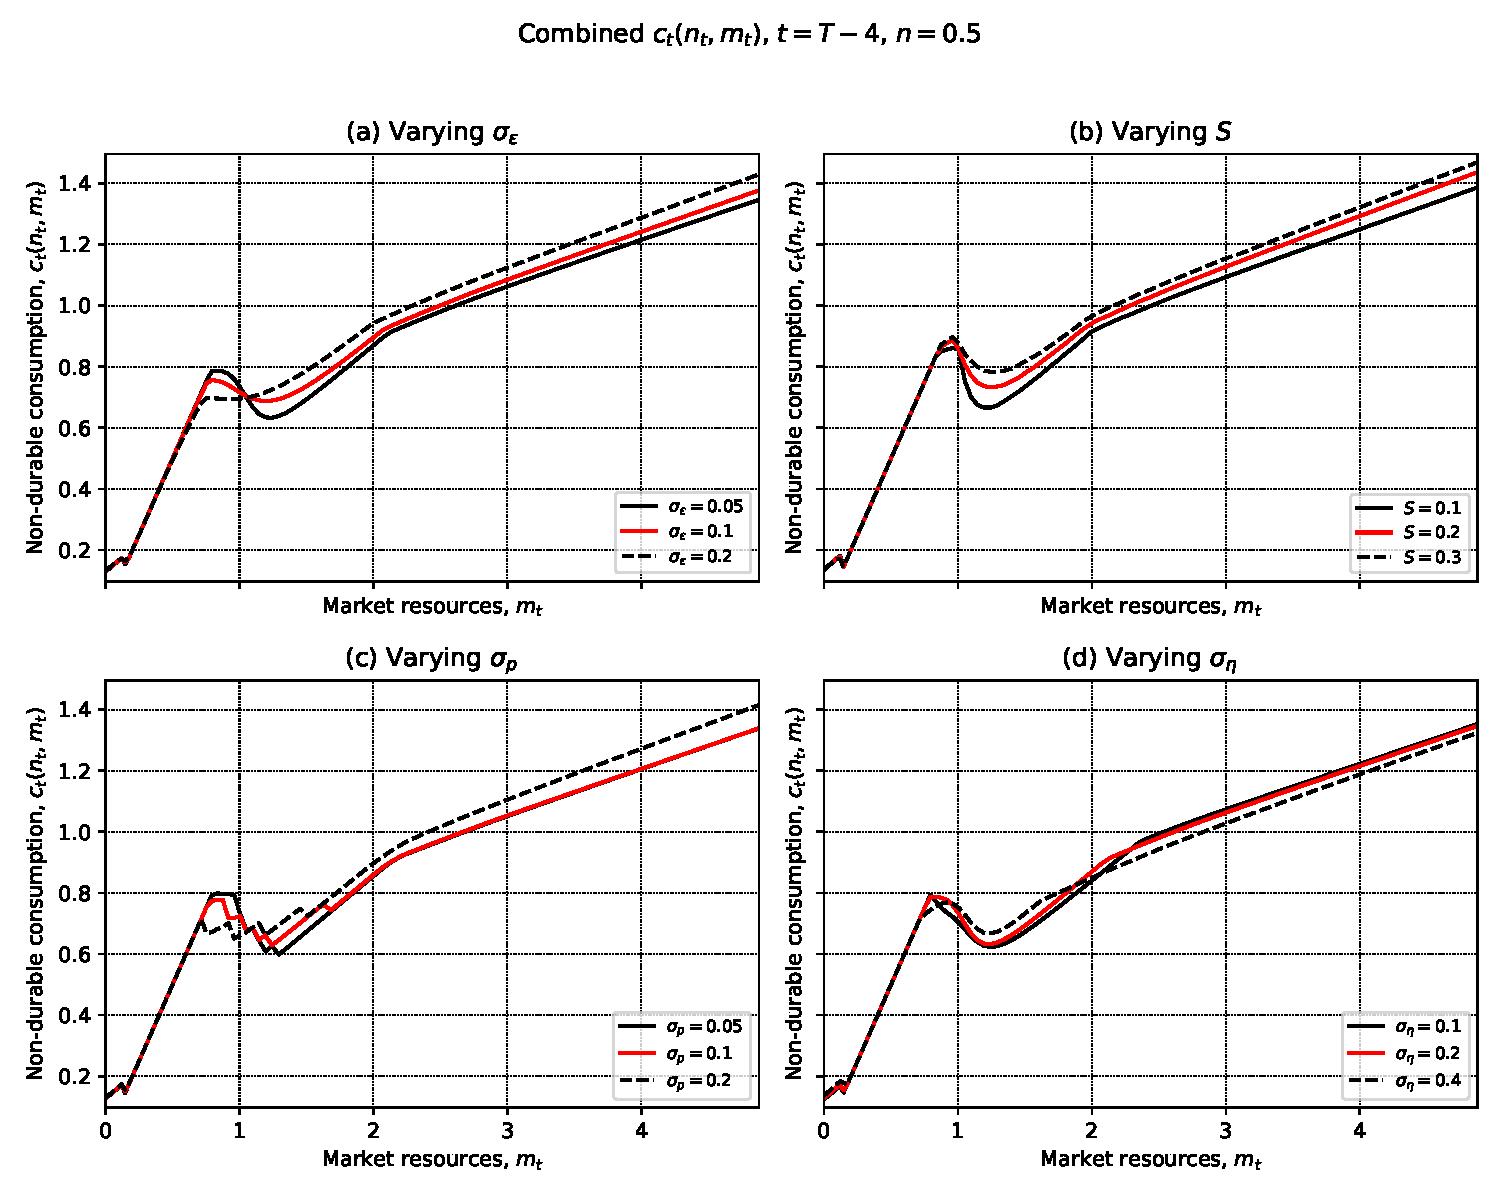
\includegraphics[width=\linewidth]{../../Figures/DurableModel/SmoothingShifts_c_periodt.pdf}
		\caption{Combined nondurable consumption $c_t(n_0,m_t)$.}
		\label{fig:smoothing_shifts_c}
	\end{subfigure}
	\hfill
	\begin{subfigure}{0.48\textwidth}
		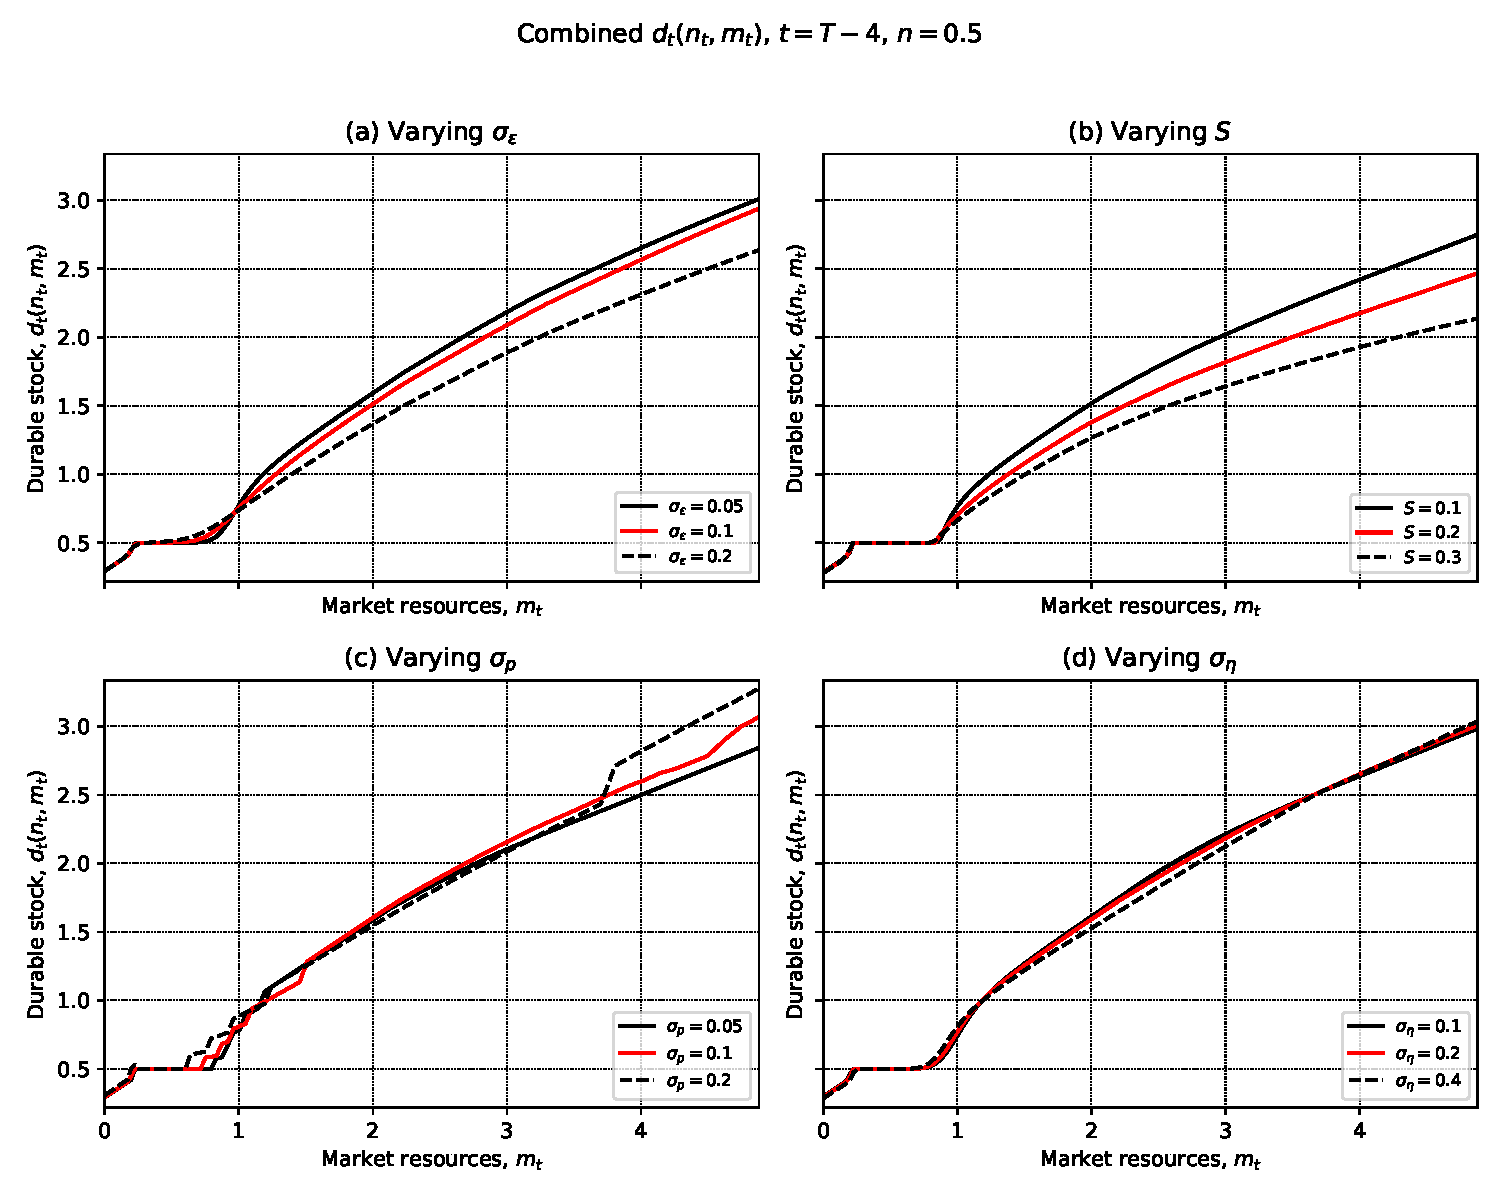
\includegraphics[width=\linewidth]{../../Figures/DurableModel/SmoothingShifts_d_periodt.pdf}
		\caption{Combined durable stock $d_t(n_0,m_t)$.}
		\label{fig:smoothing_shifts_d}
	\end{subfigure}
	\caption{Combined policies at fixed $n_0$ when each smoothness channel is strengthened. Panels vary (a)~$\sigma_\varepsilon$, (b)~$S$, (c)~$\sigma_p$, and (d)~$\sigma_\eta$. All four raise $c_t$ and lower $d_t$ relative to the lightly smoothed reference in that panel.}
	\label{fig:smoothing_shifts_levels}
\end{figure}

\begin{figure}[htbp]
	\centering
	\begin{subfigure}{0.48\textwidth}
		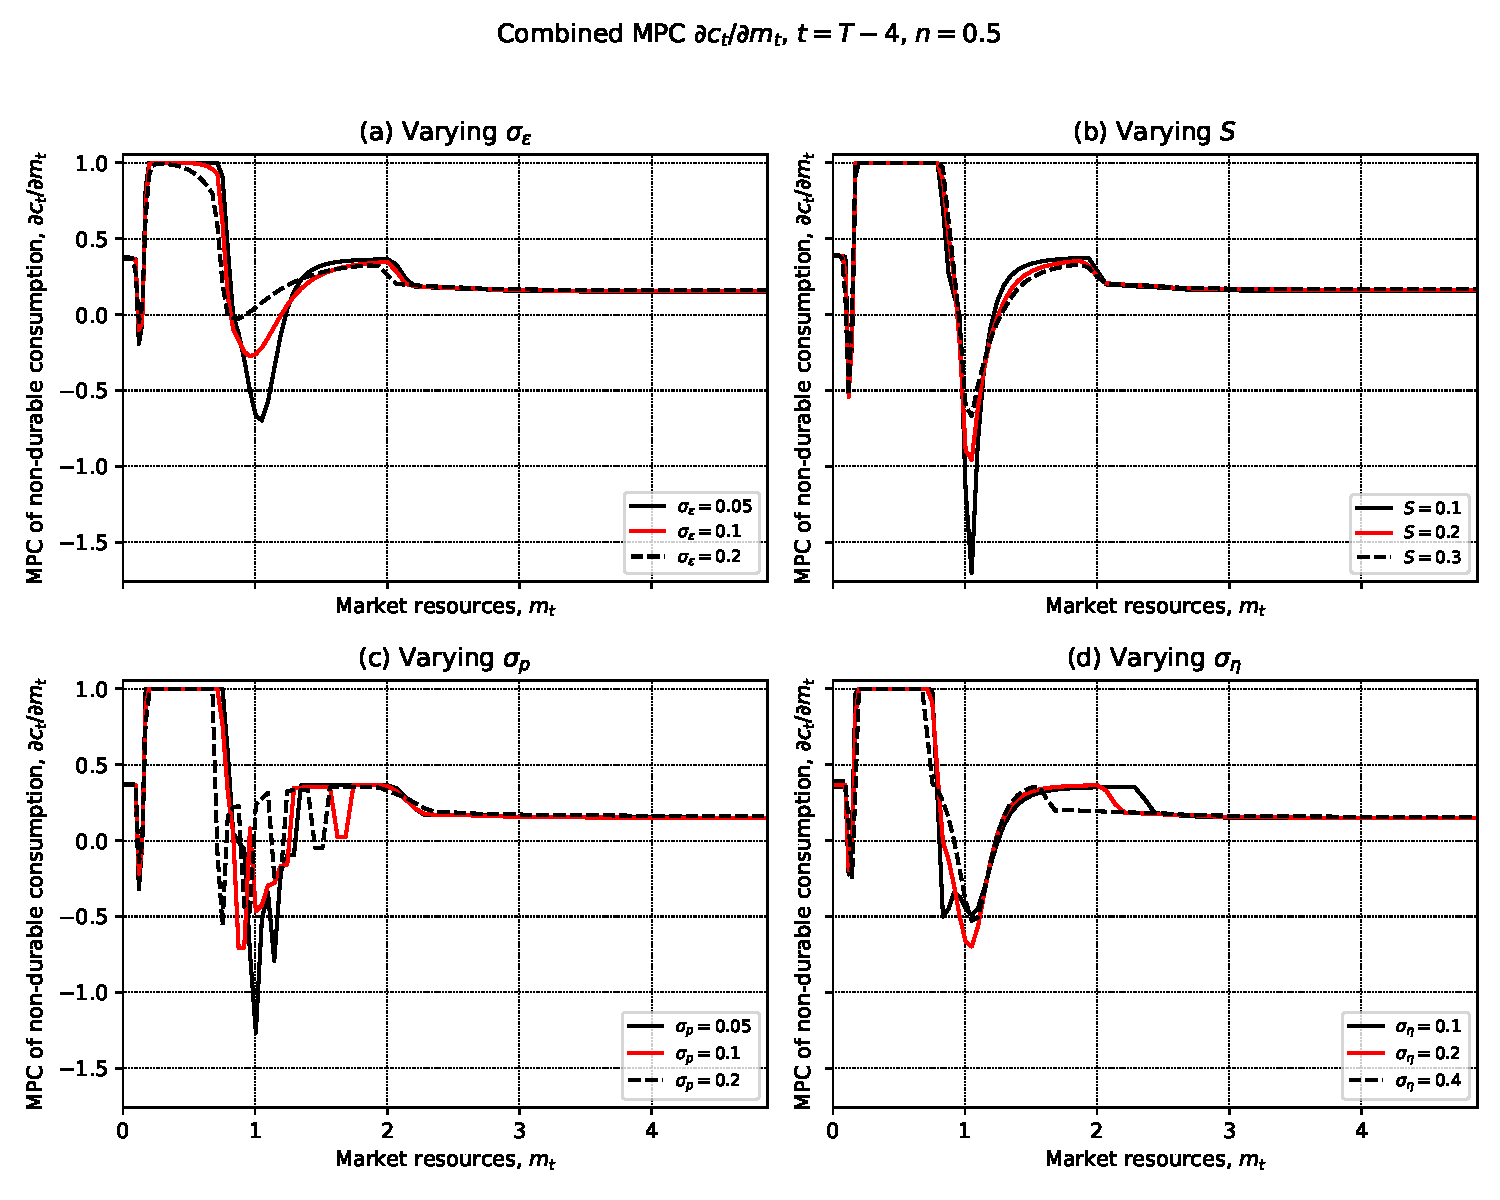
\includegraphics[width=\linewidth]{../../Figures/DurableModel/SmoothingShifts_c_MPC_periodt.pdf}
		\caption{MPC of nondurable consumption $\partial c_t/\partial m_t$.}
		\label{fig:smoothing_shifts_c_MPC}
	\end{subfigure}
	\hfill
	\begin{subfigure}{0.48\textwidth}
		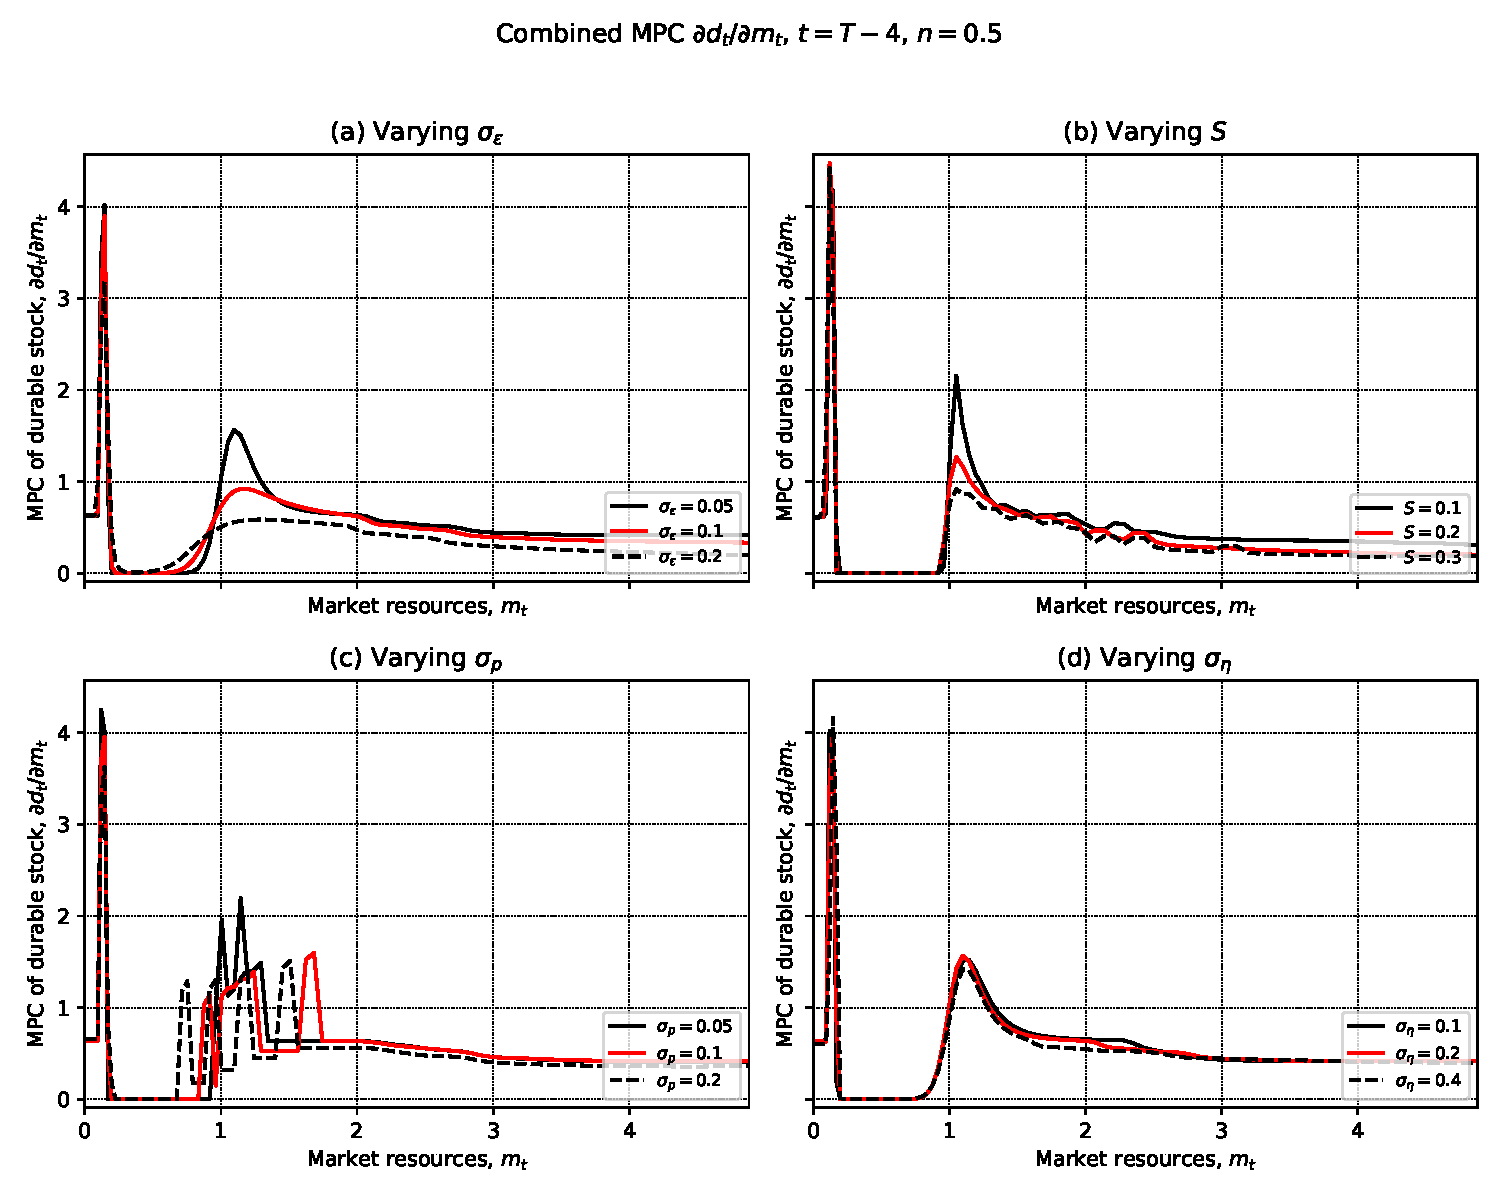
\includegraphics[width=\linewidth]{../../Figures/DurableModel/SmoothingShifts_d_MPC_periodt.pdf}
		\caption{MPC of durable stock $\partial d_t/\partial m_t$.}
		\label{fig:smoothing_shifts_d_MPC}
	\end{subfigure}
	\caption{Combined MPCs at fixed $n_0$ under the same four experiments as Figure~\ref{fig:smoothing_shifts_levels}. Strengthening any channel dampens the spikes around the S,s band.}
	\label{fig:smoothing_shifts_mpcs}
\end{figure}

\subsection{Comparing smoothness mechanisms: Infinite horizon}
\label{subsec:ModelBasicInf}

The comparisons above are period-$t$ objects on a fixed beginning-of-period durable stock. I next ask how the same three discrete-choice smoothers---EV taste shocks $\sigma_\varepsilon$, search frictions $S$, and durable-price dispersion $\sigma_p$---shape the \emph{stationary} economy. For each channel I solve the infinite-horizon problem with that smoother active and the other two shut off, using the same magnitudes as in Figures~\ref{fig:smoothing_shifts_levels}--\ref{fig:smoothing_shifts_mpcs}. Given the converged policies, I build the transition matrix over the joint $(n,m)$ histogram grid, compute the ergodic distribution, and report aggregate steady-state nondurable consumption $C$, durable stock $D$, durable expenditure $\mathrm{DEX}$, total expenditure $\mathrm{TEX}$, liquid assets $A$, and the adjustment probability $\mathrm{ADJ}$.

I also compute sequence-space Jacobians of these aggregates with respect to the risk-free return $R$ and to a labor (mean-income) shock, using the fake-news algorithm for sequence-space Jacobians; the labor Jacobians are reported separately below. Table~\ref{tab:inf_ss} reports the steady-state aggregates.

\begin{table}[htbp]
\centering
\caption{Infinite-horizon steady-state aggregates: EV taste shocks $\sigma_\varepsilon$, and search+price with either $\sigma_p$ varied at $S=0.2$ or $S$ varied at $\sigma_p=0.1$.}
\label{tab:inf_ss}
\footnotesize
\begin{tabular}{llcccccc}
\hline
 &  & \multicolumn{6}{c}{Steady state} \\
\cline{3-8}
 &  & $C$ & $D$ & $\mathrm{DEX}$ & $\mathrm{TEX}$ & $A$ & $\mathrm{ADJ}$ (\%) \\
\hline
\multirow{3}{*}{$\sigma_\zeta$} & $0.1$ & $0.80$ & $3.56$ & $0.18$ & $0.97$ & $0.94$ & $12.2$ \\
 & $0.15$ & $0.79$ & $3.27$ & $0.16$ & $0.95$ & $0.71$ & $18.6$ \\
 & $0.2$ & $0.79$ & $3.03$ & $0.15$ & $0.94$ & $0.60$ & $24.7$ \\
\addlinespace
\multirow{3}{*}{$\sigma_p$ ($S=0.2$)} & $0.08$ & $0.81$ & $4.28$ & $0.21$ & $1.03$ & $1.39$ & $7.7$ \\
 & $0.1$ & $0.81$ & $4.51$ & $0.23$ & $1.04$ & $1.32$ & $8.7$ \\
 & $0.12$ & $0.82$ & $4.87$ & $0.24$ & $1.06$ & $1.27$ & $9.9$ \\
\addlinespace
\multirow{3}{*}{$S$ ($\sigma_p=0.1$)} & $0.15$ & $0.81$ & $4.59$ & $0.23$ & $1.04$ & $1.27$ & $9.3$ \\
 & $0.2$ & $0.81$ & $4.51$ & $0.23$ & $1.04$ & $1.32$ & $8.7$ \\
 & $0.25$ & $0.81$ & $4.45$ & $0.22$ & $1.04$ & $1.37$ & $8.3$ \\
\hline
\end{tabular}

\end{table}

\paragraph{Results.}

All numerical smoothing mechanisms also smooth consumption policy functions. As a result, both the steady state non-durable consumption, and durable expenditure reduce with higher smoothing intensity. The flip site are slightly larger asset holdings. One key divergence is the share of adjuster. A larger taste shock leads to more households who exogenously want to adjust. For prices, we get a larger share as well, but for a different reason. Higher price dispersion lead to cheaper durable goods and hence, households who draw a lucky price draw adjust more frequently. The opposite is true for search. With a higher search friction, households start searching earlier, but the intensity reduces which leads to a lower share of adjusters. Therefore, when we want to target MPC or MPX, all three measures lead to a dampened number. But when we also want to target the share of adjusters, taste and price shocks lead to the opposite effect of search frictions.

\paragraph{Kinks and Euler residuals}
\label{subsec:ModelBasicEuler}

Table~\ref{tab:smoothing_kinks} records cleanliness of the raw EGM cloud. The object that is stored and plotted is an interpolant of the refined cloud, so a zero deletion count does not by itself establish that the computed rule solves the problem that was posed. A policy mixed over dominated Euler roots can look as smooth as one whose envelope has nothing left to delete. I therefore pair the kink counts with off-grid Euler residuals in the sense of \citet{Judd1992-sp}. For an unconstrained continuous choice $c$ with implied Euler consumption $c^{\mathrm{impl}}$,
\begin{align}
	\mathrm{EE}(c)
	\;=\;
	\log_{10}\!\left(
		\left\lvert \frac{c - c^{\mathrm{impl}}}{c} \right\rvert
		+ 10^{-16}
	\right).
	\label{eq:judd_ee}
\end{align}
More negative is more accurate: $-4$ is a $0.01\%$ consumption error, $-3$ a $0.1\%$ error. Residuals are branch-conditional---keepers on $c_t^{\mathrm{keep}}$, adjusters on the durable first-order condition converted to the same consumption units ($\mathrm{EE}_d^{\mathrm{adj}}$)---and are never evaluated at the mixed policy $\bar c_t$, which does not satisfy the Euler equation even when both branches do. The test mesh is off the solution grid; constrained points are dropped. I report the mean and the 95th percentile, because the mean can look acceptable while a thin set of points near the S,s band is not.

Table~\ref{tab:smoothing_euler} places both diagnostics in the same period as Figures~\ref{fig:smoothing_shifts_levels}--\ref{fig:smoothing_shifts_mpcs}, now for every listed magnitude of $\sigma_\varepsilon$, $S$, and $\sigma_p$. For the keeper the computational claim holds. Decreasing segments are zero at all three taste and search values, and $\mathrm{EE}_c^{\mathrm{keep}}$ improves with the smoother: the hard-max mean and 95th percentile are $-4.19$ and $-2.50$; at $\sigma_\varepsilon=0.2$ they are $-4.52$ and $-3.39$, and at $S=0.3$ they are $-4.42$ and $-3.24$. The smoother combined consumption rule is not an average over dominated keeper roots. Price dispersion likewise zeros the keeper count at all three $\sigma_p$, with only a small deterioration in the mean (from $-4.11$ at $\sigma_p=0.05$ to $-4.00$ at $0.2$).

For the adjuster the deletion count is not enough. Taste and search eliminate FUES removals at every listed magnitude, but the 95th percentile of $\mathrm{EE}_d^{\mathrm{adj}}$ remains positive---$0.45$ to $0.69$ as $\sigma_\varepsilon$ rises, $0.27$ to $0.22$ as $S$ rises---while the mean stays around $-3$. Raising the smoother does not repair the tail. Price dispersion continues to remove points ($20$, $17$, $34$ as $\sigma_p$ increases) and has a similar tail. Cleanliness of the raw FOC cloud is not the same as accuracy of the stored $(c,d)$ interpolant, so FUES is not shown to be redundant by the deletion count alone. Taste, search, and prices are different economies and are not ranked by residual size; the residuals certify internal accuracy of each specification, not proximity to the frictionless target. Table~\ref{tab:smoothing_euler_inf} reports the same kink and Euler diagnostics for the infinite-horizon stationary policies of Section~\ref{subsec:ModelBasicInf}.

\begin{table}[htbp]
\centering
\caption{Period-$t$ kink counts and Euler residuals under the hard-max baseline and the same $\sigma_\varepsilon$, $S$, and $\sigma_p$ sweep as Figure~\ref{fig:smoothing_shifts_levels}. Residuals are mean and 95th percentile of~\eqref{eq:judd_ee} on an off-grid test mesh; constrained points excluded. The $\sigma_p$ adjuster kink count sums over price nodes.}
\label{tab:smoothing_euler}
\small
\begin{tabular}{llcccccc}
\hline
 &  & \multicolumn{2}{c}{Kinks} & \multicolumn{2}{c}{$\mathrm{EE}_c^{\mathrm{keep}}$} & \multicolumn{2}{c}{$\mathrm{EE}_d^{\mathrm{adj}}$} \\
\cline{3-4}\cline{5-6}\cline{7-8}
 &  & Decr.\ seg. & FUES rem. & Mean & P95 & Mean & P95 \\
\hline
\multicolumn{2}{l}{Hard max} & 5 & 4 & $-4.19$ & $-2.50$ & $-3.49$ & $-2.42$ \\
\addlinespace
\multirow{3}{*}{$\sigma_\zeta$} & $0.05$ & 0 & 0 & $-4.22$ & $-3.23$ & $-3.04$ & $0.45$ \\
 & $0.1$ & 0 & 0 & $-4.39$ & $-3.32$ & $-3.03$ & $0.48$ \\
 & $0.2$ & 0 & 0 & $-4.52$ & $-3.39$ & $-3.25$ & $0.69$ \\
\addlinespace
\multirow{3}{*}{$S$} & $0.1$ & 0 & 0 & $-4.23$ & $-3.13$ & $-3.06$ & $0.27$ \\
 & $0.2$ & 0 & 0 & $-4.34$ & $-3.21$ & $-3.22$ & $0.22$ \\
 & $0.3$ & 0 & 0 & $-4.42$ & $-3.24$ & $-3.20$ & $0.22$ \\
\addlinespace
\multirow{3}{*}{$\sigma_p$} & $0.05$ & 0 & 20 & $-4.11$ & $-2.92$ & $-2.96$ & $0.53$ \\
 & $0.1$ & 0 & 17 & $-4.04$ & $-2.93$ & $-2.97$ & $0.52$ \\
 & $0.2$ & 0 & 34 & $-4.00$ & $-2.94$ & $-2.87$ & $0.65$ \\
\hline
\end{tabular}

\end{table}

\begin{table}[htbp]
\centering
\caption{Infinite-horizon kink counts and Euler residuals under the same $\sigma_\varepsilon$, $S$, and $\sigma_p$ sweep as Figure~\ref{fig:smoothing_shifts_levels} and Table~\ref{tab:inf_ss}. Each channel is varied with the other two shut off. Residuals are mean and 95th percentile of~\eqref{eq:judd_ee} on an off-grid test mesh evaluated at the stationary policy; constrained points excluded. The $\sigma_p$ adjuster kink count sums over price nodes.}
\label{tab:smoothing_euler_inf}
\small
\begin{tabular}{llcccccc}
\hline
 &  & \multicolumn{2}{c}{Kinks} & \multicolumn{2}{c}{$\mathrm{EE}_c^{\mathrm{keep}}$} & \multicolumn{2}{c}{$\mathrm{EE}_d^{\mathrm{adj}}$} \\
\cline{3-4}\cline{5-6}\cline{7-8}
 &  & Decr.\ seg. & FUES rem. & Mean & P95 & Mean & P95 \\
\hline
\multirow{3}{*}{$\sigma_\zeta$} & $0.1$ & 0 & 0 & $-5.08$ & $-4.09$ & $-1.49$ & $1.35$ \\
 & $0.15$ & 0 & 0 & $-5.20$ & $-4.15$ & $-1.92$ & $0.94$ \\
 & $0.2$ & 0 & 0 & $-5.29$ & $-4.17$ & $-2.17$ & $0.66$ \\
\addlinespace
\multirow{3}{*}{$S$} & $0.15$ & 1 & 0 & $-3.59$ & $-2.23$ & $-1.24$ & $1.59$ \\
 & $0.2$ & 0 & 0 & $-3.89$ & $-2.64$ & $-2.24$ & $0.50$ \\
 & $0.25$ & 0 & 0 & $-4.80$ & $-3.60$ & $-2.05$ & $0.53$ \\
\addlinespace
\multirow{3}{*}{$\sigma_p$} & $0.05$ & 0 & 102 & $-4.76$ & $-3.31$ & $-1.89$ & $1.24$ \\
 & $0.1$ & 0 & 59 & $-5.01$ & $-3.83$ & $-2.73$ & $0.10$ \\
 & $0.15$ & 1 & 22 & $-4.92$ & $-3.87$ & $-3.20$ & $-1.00$ \\
\addlinespace
\multirow{3}{*}{$\sigma_p$ ($S=0.2$)} & $0.08$ & 0 & 55 & $-4.88$ & $-3.86$ & $-2.12$ & $1.21$ \\
 & $0.1$ & 0 & 48 & $-4.89$ & $-3.82$ & $-2.08$ & $1.31$ \\
 & $0.12$ & 2 & 35 & $-4.92$ & $-3.81$ & $-2.25$ & $0.99$ \\
\addlinespace
\multirow{3}{*}{$S$ ($\sigma_p=0.1$)} & $0.15$ & 0 & 64 & $-4.62$ & $-3.27$ & $-2.11$ & $1.08$ \\
 & $0.2$ & 0 & 48 & $-4.89$ & $-3.82$ & $-2.08$ & $1.31$ \\
 & $0.25$ & 0 & 49 & $-4.89$ & $-3.84$ & $-2.20$ & $1.10$ \\
\hline
\end{tabular}

\end{table}

\paragraph{Jacobians}
Using the smoothing mechanism also allows us to calculate Jacobians smoother:

\begin{figure}[htbp]
	\centering
	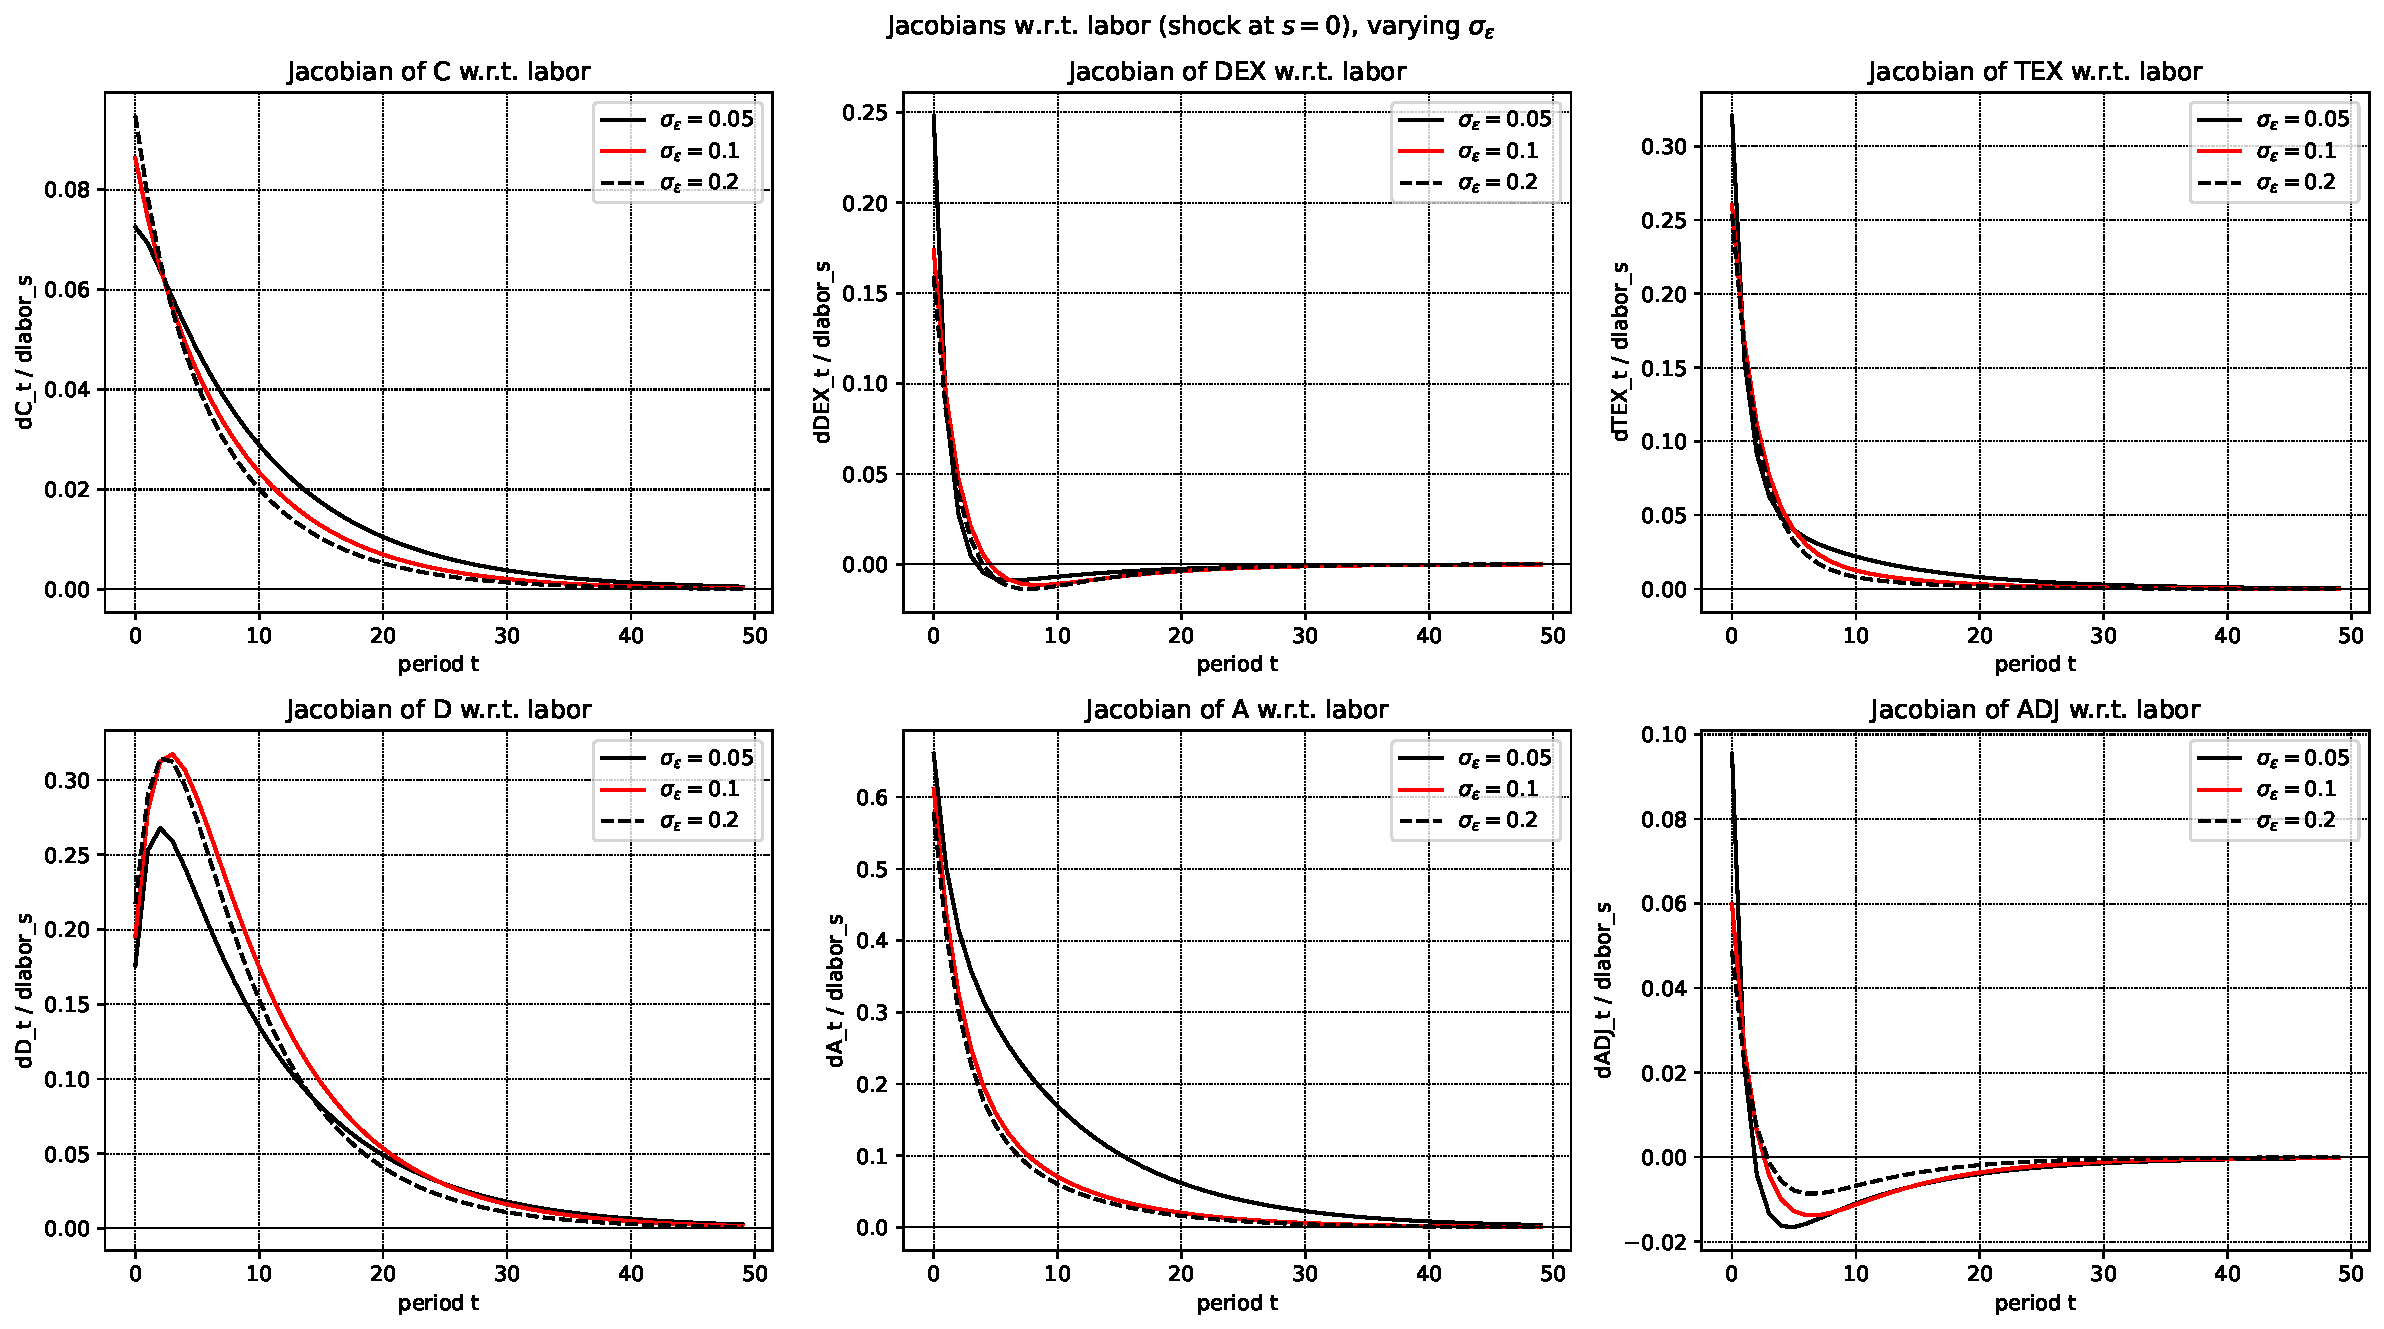
\includegraphics[width=0.85\linewidth]{../../Figures/DurableModel/Taste_Inf_Jacobians_labor.pdf}
	\caption{Jacobians wrt labor varying taste intensity.}
	\label{fig:Taste_Inf_Jacobians_labor}
\end{figure}

\begin{figure}[htbp]
	\centering
	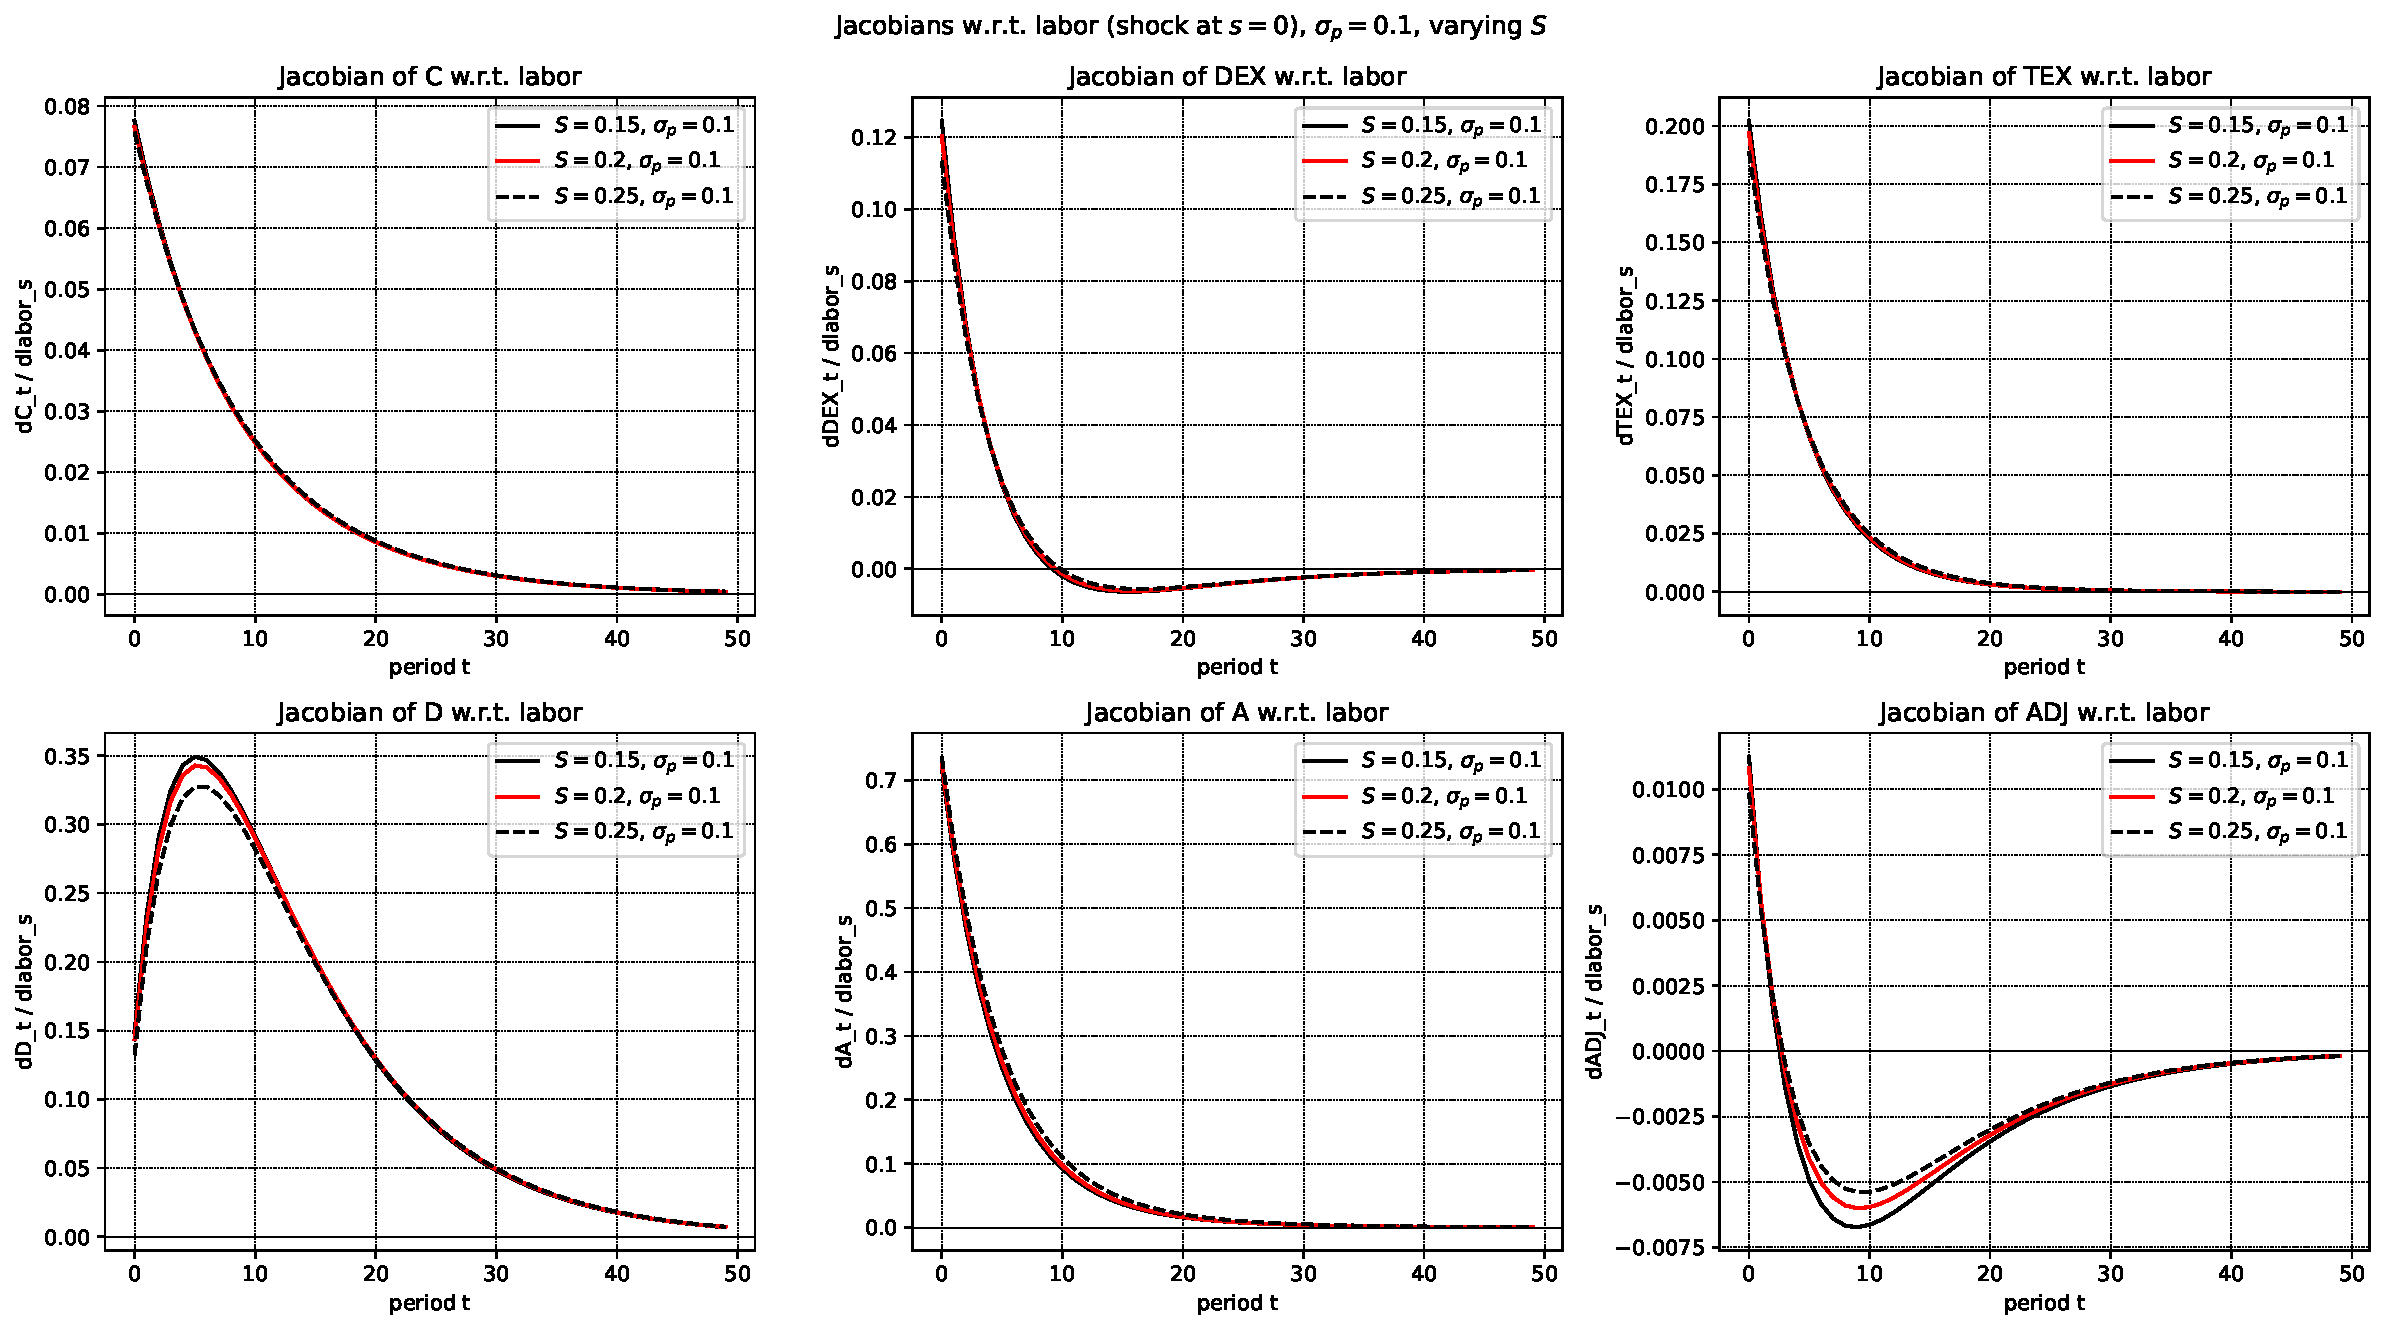
\includegraphics[width=0.85\linewidth]{../../Figures/DurableModel/Combined_varS_Inf_Jacobians_labor.pdf}
	\caption{Jacobians wrt labor varying search intensity.}
	\label{fig:Combined_varS_Inf_Jacobians_labor}
\end{figure}

\begin{figure}[htbp]
	\centering
	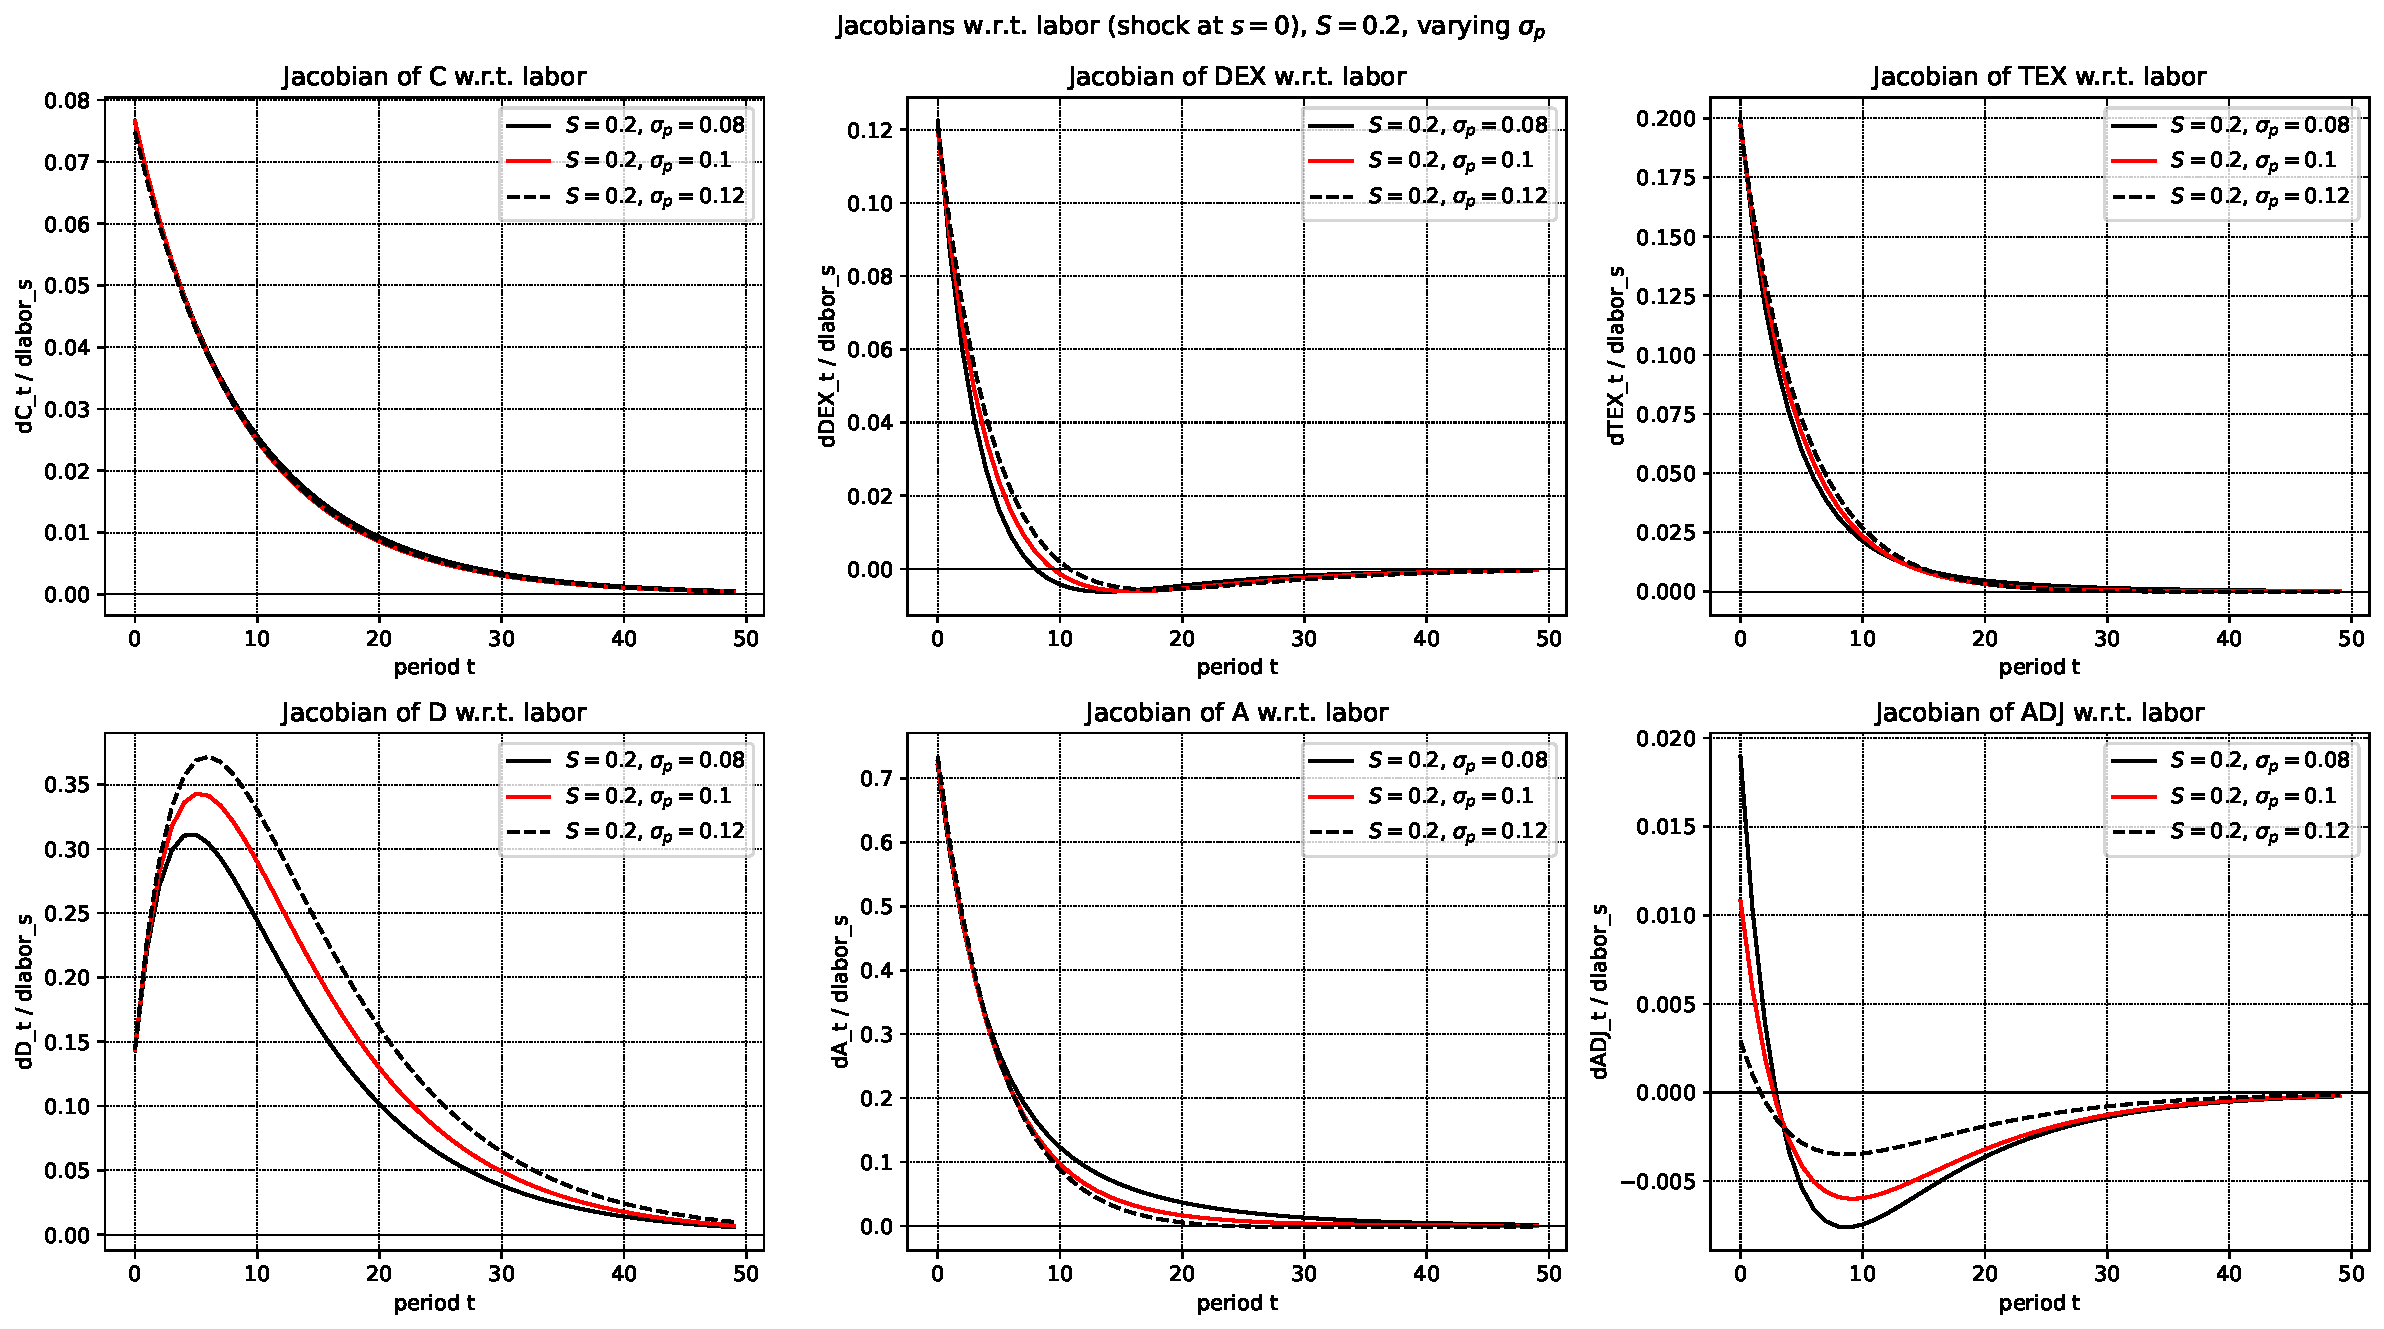
\includegraphics[width=0.85\linewidth]{../../Figures/DurableModel/Combined_varP_Inf_Jacobians_labor.pdf}
	\caption{Jacobians wrt labor varying price dispersion.}
	\label{fig:Combined_varS_InP_Jacobians_labor}
\end{figure}


%============================================================
\section{Conclusion}\label{sec:Conclusion}
%============================================================
This paper introduces search as a new method for smoothing out discrete-continuous
choice (DC) problems. While search can significantly reduce the size of the disconti-
nuities in the decision rule of a DC problem, to get uniform smoothness around the
discontinuities, we need to incorporate taste shocks as well. Together, search and taste
shocks offer modelers greater control over the degree of smoothness in DC models, while
rationalizing the smoothness into the agent's choice problem. With ample smoothness,
discontinuities in the decision rule can be smoothed out entirely; thus, eliminating the
need for incorporating an additional, computationally costly, step of identifying and
removing suboptimal points generated in the EGM step for DC models. This paper
studies search in the context of a consumption-saving-retirement problem; however, the
framework can be easily applied to models of housing purchase, lumpy firm investments,
and a wide array of other DC models.
We additionally document how a coarse income-shock discretization injects phantom
kinks into the decision rule, and describe a transition-matrix method that integrates
the continuous income density and removes those numerical artifacts at moderate cost.


%============================================================
% References
%============================================================
\bibliographystyle{plainnat}
\bibliography{References_v3}

\clearpage
%============================================================
% Appendices
%============================================================
\appendix

%============================================================
\section{Retirement-model appendix}\label{sec:appdx_retirement}
%============================================================
This appendix derives the objects used in Sections~\ref{sec:RetirementModel} and~\ref{sec:RetirementModelPrices}. Section~\ref{subsec:appdx_ret_baseline} records the baseline envelopes and Euler equations (no account-value risk). Section~\ref{subsec:appdx_ret_price} introduces stochastic retirement-account realizations in isolation. Section~\ref{subsec:appdx_ret_full} nests those realizations with directed search.

%------------------------------------------------------------
\subsection{Baseline envelopes and Euler equations}\label{subsec:appdx_ret_baseline}
%------------------------------------------------------------
The environment is that of Section~\ref{sec:RetirementModel}: log utility, disutility of work $\delta$, convex search cost $\theta(\eff_t)=\sigma_s\bigl(\eff_t+(1-\eff_t)\log(1-\eff_t)\bigr)$, option probabilities $P_1(\eff_t)=(1-\eff_t)p+\eff_t$ and $P_2(\eff_t)=(1-\eff_t)(1-p)$, and $M_{t+1}=A_t R+y_{t+1}d_t$ with $y_{t+1}=y\eta_{t+1}$. Claiming delivers book resources one-for-one, so both branches use $A_t=M_t-c_t$.

\paragraph{Retiree.}
Retirement is self-absorbing. The Bellman equation is
\begin{align}
	V_t^{\Ret}(M_t)
	&= \max_{0\le c_t\le M_t}
	\left\{
		\log(c_t)+\beta V_{t+1}^{\Ret}(A_t R)
	\right\},
	\qquad A_t=M_t-c_t.
\end{align}
The Lagrangian $\mathscr{L}=\log(c_t)+\beta V_{t+1}^{\Ret}(A_t R)+\lambda_t^{\Ret}(M_t-c_t-A_t)$ yields
\begin{align}
	\lambda_t^{\Ret} = \frac{1}{c_t}
	= \beta R\,\frac{\partial V_{t+1}^{\Ret}(A_t R)}{\partial M_{t+1}}.
\end{align}
The envelope theorem gives $\partial V_t^{\Ret}/\partial M_t=\lambda_t^{\Ret}=1/c_t^{\Ret}$, which iterated forward is $\partial V_{t+1}^{\Ret}/\partial M_{t+1}=1/c_{t+1}^{\Ret}$. Substituting produces the baseline retiree Euler equation
\begin{align}
	\frac{1}{c_t}
	= R\beta\,\frac{1}{c_{t+1}^{\Ret}(A_t R)},
	\label{eq:ret_baseline_euler}
\end{align}
or $c_t^{\Ret}=\bigl(R\beta(c_{t+1}^{\Ret}(A_t R))^{-1}\bigr)^{-1}$, as in the main text. The gothic retiree value is $\goth{V}_t^{\Ret}(A_t)\equiv V_{t+1}^{\Ret}(A_t R)$. This retiree problem is an input to Sections~\ref{subsec:appdx_ret_price}--\ref{subsec:appdx_ret_full}: a claimed account $\tilde M=\phi M$ is just a different starting point for the same functions $V_t^{\Ret}$ and $c_t^{\Ret}$.

\paragraph{Worker who must work.}
With the taste shock $\xi_t$ outside the inner maximum, as in Section~\ref{sec:RetirementModel},
\begin{align}
	V_t^{W}(M_t,\xi_t)
	&= \xi_t\max_{\substack{0\le c_t\le M_t\\ 0\le\eff_t\le 1}}
	\left\{
		\log(c_t)-\delta-\theta(\eff_t)
		+\beta P_1(\eff_t)\,\goth{V}_t^{1}(A_t)
		+\beta P_2(\eff_t)\,\goth{V}_t^{2}(A_t)
	\right\}.
	\label{eq:ret_baseline_VW}
\end{align}
Splitting consumption and effort into sequential sub-periods, the effort first-order condition is
\begin{align}
	\theta'(\eff_t^{\ast})
	&= \beta(1-p)\bigl(\goth{V}_t^{1}(A_t)-\goth{V}_t^{2}(A_t)\bigr),
\end{align}
and since $\theta'(\eff)=-\sigma_s\log(1-\eff)$,
\begin{align}
	\eff_t^{\ast}(A_t)
	&= 1-\exp\left(
		-\frac{\beta(1-p)}{\sigma_s}
		\bigl(\goth{V}_t^{1}(A_t)-\goth{V}_t^{2}(A_t)\bigr)
	\right).
	\label{eq:ret_baseline_effort}
\end{align}
The consumption first-order condition, evaluated at $\eff_t^{\ast}$, is
\begin{align}
	\frac{1}{c_t}
	&= \beta\left[
		P_1(\eff_t^{\ast})\,\frac{\partial\goth{V}_t^{1}}{\partial A_t}
		+P_2(\eff_t^{\ast})\,\frac{\partial\goth{V}_t^{2}}{\partial A_t}
	\right].
	\label{eq:ret_baseline_foc_c}
\end{align}
Differentiating the gothic values,
\begin{align}
	\frac{\partial\goth{V}_t^{1}}{\partial A_t}
	&= R\,\mathbb{E}_t\left[
		\frac{\partial V_{t+1}^{R,W}(M_{t+1},\xi_{t+1})}{\partial M_{t+1}}
	\right],
	\\
	\frac{\partial\goth{V}_t^{2}}{\partial A_t}
	&= R\,\mathbb{E}_t\left[
		\frac{\partial V_{t+1}^{W}(M_{t+1},\xi_{t+1})}{\partial M_{t+1}}
	\right],
\end{align}
where the expectation is over $(y_{t+1},\xi_{t+1})$. The envelope theorem applied to~\eqref{eq:ret_baseline_VW}, using that $\eff_t^{\ast}$ is already optimal so its indirect effect vanishes, gives
\begin{align}
	\frac{\partial V_t^{W}(M_t,\xi_t)}{\partial M_t}
	&= \xi_t\cdot\frac{1}{c_t^{W}}
	= \xi_t\,u'(c_t^{W},1,\eff_t^{\ast}).
	\label{eq:ret_baseline_env_W}
\end{align}
For the worker who has the option,
\begin{align}
	V_t^{R,W}(M_t,\xi_t)
	&= \max\big\{V_t^{\Ret}(M_t),\; V_t^{W}(M_t,\xi_t)\big\},
\end{align}
so
\begin{align}
	\frac{\partial V_{t+1}^{R,W}}{\partial M_{t+1}}
	&= \mathbbm{1}_{t+1}^{0}\cdot\frac{1}{c_{t+1}^{\Ret}}
	+\mathbbm{1}_{t+1}^{1}\cdot\xi_{t+1}\cdot\frac{1}{c_{t+1}^{W}},
	\label{eq:ret_baseline_env_RW}
\end{align}
with $\mathbbm{1}_{t+1}^{0}=1$ iff $V_{t+1}^{\Ret}\ge V_{t+1}^{W}$ and $\mathbbm{1}_{t+1}^{1}=1-\mathbbm{1}_{t+1}^{0}$. Substituting~\eqref{eq:ret_baseline_env_W}--\eqref{eq:ret_baseline_env_RW} into~\eqref{eq:ret_baseline_foc_c} recovers the worker consumption function in the main text.

\paragraph{Terminal period.}
With $V_{T+1}\equiv 0$ and no borrowing, both branches set $A_T=0$. The retiree consumes $c_T^{\Ret}=M_T$ and $V_T^{\Ret}=\log(M_T)$. The worker consumes $c_T^{W}=M_T$ and $V_T^{W}(M_T,\xi_T)=\xi_T\bigl(\log(M_T)-\delta\bigr)$ (effort is irrelevant because there is no $T+1$). The option-contingent value is the hard maximum of the two.

%------------------------------------------------------------
\subsection{Derivations: Stochastic retirement wealth (Section~\ref{subsec:RetirementPrices})}\label{subsec:appdx_ret_price}
%------------------------------------------------------------
This subsection derives the envelope conditions, the Euler equations, the terminal-period solution, and the EGM algorithm for the account-realization extension of Section~\ref{subsec:RetirementPrices}. Taste shocks and search are shut down ($p=1$, $\sigma_\xi=0$, $\eff_t\equiv 0$). The retiree's Bellman problem, first-order condition, and envelope of Section~\ref{subsec:appdx_ret_baseline} carry over unchanged: once a draw has been accepted, the agent is an ordinary retiree starting from $\tilde M_t=\phi_t M_t$. The worker's budget remains $A_t=M_t-c_t$. What changes is the discrete comparison and, through that comparison, the continuation that enters the worker's Euler equation.

\paragraph{Claiming maps into the baseline retiree.}
Define claimed wealth by~\eqref{eq:ret_price_Mtilde}, $\tilde M_t=\phi_t M_t$. The value of accepting the draw is the baseline retiree value evaluated at that point,
\begin{align}
	V_t^{\mathrm{claim}}(M_t,\phi_t)
	&\equiv V_t^{\Ret}(\phi_t M_t),
	\label{eq:ret_price_Vclaim}
\end{align}
with claiming-period consumption $c_t^{\mathrm{claim}}(M_t,\phi_t)=c_t^{\Ret}(\phi_t M_t)$. The retiree Euler equation remains~\eqref{eq:ret_baseline_euler}; $\phi_t$ does not appear in it. After claiming, $A_t=\phi_t M_t-c_t^{\Ret}(\phi_t M_t)$ and $M_{t+1}=A_t R$, with no further account draws.

\paragraph{Envelope conditions.}
By the chain rule, the derivative of claiming value with respect to \emph{book} resources $M_t$, holding $\phi_t$ fixed, is
\begin{align}
	\frac{\partial V_t^{\mathrm{claim}}(M_t,\phi_t)}{\partial M_t}
	&= \phi_t\cdot\frac{\partial V_t^{\Ret}(\tilde M_t)}{\partial\tilde M_t}
	= \phi_t\cdot\frac{1}{c_t^{\Ret}(\phi_t M_t)}.
	\label{eq:ret_price_env_Ret}
\end{align}
An extra unit of book wealth is worth $\phi_t$ units of retirement wealth, each of which has marginal value $1/c_t^{\Ret}(\tilde M_t)$. Relative to the baseline envelope $\partial V_t^{\Ret}/\partial M_t=1/c_t^{\Ret}$, the right-hand side is scaled by $\phi_t$ and the consumption function is evaluated at $\phi_t M_t$ rather than at $M_t$. This is the analog of the durable-price envelope in which $p_t$ changes the adjuster's optimum: here $\phi_t$ changes the state at which that optimum is evaluated, not the first-order condition itself.

The worker never claims, so
\begin{align}
	\frac{\partial V_t^{W}(M_t)}{\partial M_t}
	&= \frac{1}{c_t^{W}(M_t)},
	\label{eq:ret_price_env_W}
\end{align}
exactly as in the baseline without taste shocks.

\paragraph{Discrete choice with a stochastic account.}
Recall the realization-contingent discrete choice~\eqref{eq:ret_price_discrete},
\begin{align}
	V_t(M_t,\phi_t)
	&= \max\Big\{V_t^{\Ret}(\phi_t M_t),\; V_t^{W}(M_t)\Big\}.
\end{align}
Define the state- and draw-contingent indicators $\mathbbm{1}_t^{0}(M_t,\phi_t)=1$ iff $V_t^{\Ret}(\phi_t M_t)\ge V_t^{W}(M_t)$ and $\mathbbm{1}_t^{1}(M_t,\phi_t)=1-\mathbbm{1}_t^{0}(M_t,\phi_t)$. Applying the envelope theorem to the outer maximum,
\begin{align}
	\frac{\partial V_t(M_t,\phi_t)}{\partial M_t}
	&= \mathbbm{1}_t^{0}\cdot\phi_t\cdot\frac{1}{c_t^{\Ret}(\phi_t M_t)}
	+\mathbbm{1}_t^{1}\cdot\frac{1}{c_t^{W}(M_t)}.
	\label{eq:ret_price_env_RW}
\end{align}
Unlike the multiplicative taste shock of Section~\ref{sec:RetirementModel}, which reweights the two branches without changing either continuous policy, $\phi_t$ affects~\eqref{eq:ret_price_env_RW} both through the indicator (the extensive margin) and through the argument of $c_t^{\Ret}$ and the factor $\phi_t$ (the intensive margin and the mark-to-market of book wealth).

\paragraph{Integrating out the account draw.}
The objects that enter the time-$(t-1)$ Euler equations are the $\phi$-integrated value and marginal-value functions
\begin{align}
	\bar V_t(M_t)
	&\equiv \mathbb{E}_{\phi_t}\big[V_t(M_t,\phi_t)\big],
	\label{eq:ret_price_barV_defn}\\
	\bar V_{M,t}(M_t)
	&\equiv \mathbb{E}_{\phi_t}\left[
		\mathbbm{1}_t^{0}\cdot\phi_t\cdot\frac{1}{c_t^{\Ret}(\phi_t M_t)}
		+\mathbbm{1}_t^{1}\cdot\frac{1}{c_t^{W}(M_t)}
	\right].
	\label{eq:ret_price_barVM}
\end{align}
Equation~\eqref{eq:ret_price_barV_defn} restates~\eqref{eq:ret_price_barV}. With $p=1$, the gothic value of a worker is $\goth{V}_{t-1}^{1}(A_{t-1})=\mathbb{E}_{\eta_t}[\bar V_t(R A_{t-1}+y_t)]$. The gothic retiree value is unchanged: $\goth{V}_{t-1}^{\Ret}(A_{t-1})=V_t^{\Ret}(R A_{t-1})$, because a household that has already claimed no longer faces $\phi$. As $\sigma_\phi\to 0$, $\phi_t\to 1$ a.s., $\mathbbm{1}_t^{0}\to\mathbbm{1}\{V_t^{\Ret}(M_t)\ge V_t^{W}(M_t)\}$, and~\eqref{eq:ret_price_barVM} collapses to the baseline hard-maximum envelope~\eqref{eq:ret_baseline_env_RW} without taste shocks.

The model's ex-ante ($\phi$-weighted) consumption function follows the same logic. Because the household observes $\phi_t$ before choosing, the realized policy for a given draw is a hard 0/1 choice,
\begin{align}
	c_t(M_t,\phi_t)
	&= \mathbbm{1}_t^{0}\,c_t^{\Ret}(\phi_t M_t)
	+\mathbbm{1}_t^{1}\,c_t^{W}(M_t),
\end{align}
while the ex-ante policy reported for plotting is
\begin{align}
	\bar c_t(M_t)
	&\equiv \mathbb{E}_{\phi_t}\big[c_t(M_t,\phi_t)\big]
	= \mathbb{E}_{\phi_t}\Big[
		\mathbbm{1}_t^{0}\,c_t^{\Ret}(\phi_t M_t)
		+\mathbbm{1}_t^{1}\,c_t^{W}(M_t)
	\Big].
	\label{eq:ret_price_barc}
\end{align}

\paragraph{Euler equations.}
The retiree's Euler equation is the baseline~\eqref{eq:ret_baseline_euler}, evaluated at whatever claimed wealth the household accepted. For the worker, with $p=1$ so that $P_1=1$ and $P_2=0$,
\begin{align}
	\frac{1}{c_t^{W}(A_t)}
	&= R\beta\,\mathbb{E}_t\big[\bar V_{M,t+1}(M_{t+1})\big]
	= R\beta\int_{y_{t+1}}\int_{\phi_{t+1}}
	\left[
		\mathbbm{1}_{t+1}^{0}\cdot\phi_{t+1}\cdot\frac{1}{c_{t+1}^{\Ret}(\phi_{t+1} M_{t+1})}
		+\mathbbm{1}_{t+1}^{1}\cdot\frac{1}{c_{t+1}^{W}(M_{t+1})}
	\right]
	dF(y_{t+1})\,dF(\phi_{t+1}),
	\label{eq:ret_price_euler_W}
\end{align}
where $\mathbbm{1}_{t+1}^{0}=\mathbbm{1}_{t+1}^{0}(M_{t+1},\phi_{t+1})$, $c_{t+1}^{W}=c_{t+1}^{W}(M_{t+1})$, and $M_{t+1}=A_t R+y_{t+1}$. Relative to the baseline worker Euler, the only structural change is that the retiree-branch contribution to next period's marginal value is $\phi_{t+1}/c_{t+1}^{\Ret}(\phi_{t+1} M_{t+1})$ rather than $1/c_{t+1}^{\Ret}(M_{t+1})$, and the indicator is $\phi_{t+1}$-contingent.

\paragraph{Terminal period.}
With $V_{T+1}\equiv 0$ and borrowing prohibited, both branches set $A_T=0$. The worker's terminal solution is unaffected by the account draw: $c_T^{W}=M_T$ and $V_T^{W}=\log(M_T)-\delta$. For a claimant, $c_T^{\Ret}(\phi_T M_T)=\phi_T M_T$ and
\begin{align}
	V_T^{\Ret}(\phi_T M_T) = \log(\phi_T M_T) = \log(M_T)+\log(\phi_T).
	\label{eq:ret_price_terminal}
\end{align}
The terminal discrete choice is $V_T(M_T,\phi_T)=\max\{V_T^{\Ret}(\phi_T M_T),\,V_T^{W}(M_T)\}$. Substituting the closed forms, the household claims iff
\begin{align}
	\log(M_T)+\log(\phi_T)
	\ge \log(M_T)-\delta
	\quad\Longleftrightarrow\quad
	\phi_T \ge e^{-\delta}.
	\label{eq:ret_price_terminal_threshold}
\end{align}
The terminal extensive margin is independent of wealth: both branches consume all resources, so $M_T$ cancels and the comparison reduces to whether the log account realization exceeds the (negative of) work disutility. High $\phi_T$ favors claiming; low $\phi_T$ is denied. (In earlier periods wealth matters, because remaining at work preserves a claim on future labor income \emph{and} on future draws.) The continuation handed to period $T-1$ is $\bar V_T(M_T)=\mathbb{E}_{\phi_T}[V_T(M_T,\phi_T)]$.

\paragraph{EGM algorithm with stochastic retirement wealth.}
Let $\vec\phi=\{\phi_1,\dots,\phi_K\}$ be quadrature nodes for the log-normal account density with weights $\vec\mu=\{\mu_1,\dots,\mu_K\}$, and let $\vec\eta=\{\eta_1,\dots,\eta_J\}$ be quadrature nodes for the transitory income shock with weights $\vec\omega$, as in Algorithm~1 of Section~\ref{sec:RetirementModel}. Because $\phi_t$ rescales the state at which the baseline retiree is evaluated rather than the retiree's first-order condition, the retiree is solved \emph{once}---in contrast to the durable-price algorithm of Appendix~\ref{subsec:appdx_price_basic}, which re-solves the adjuster at every $p_k$. The algorithm for one recursive period, starting from a given next-period solution $(c_{t+1}^{\Ret},\,c_{t+1}^{W},\,V_{t+1}^{\Ret},\,V_{t+1}^{W})$, proceeds as follows.

\begin{enumerate}
	\item \textbf{Solve the retiree once,} by EGM on $A_t=\tilde M_t-c_t$ exactly as in Section~\ref{subsec:appdx_ret_baseline}, yielding $c_t^{\Ret}(\tilde M)$ and $V_t^{\Ret}(\tilde M)$ on a grid that extends to at least $\phi_{\max}M_{\max}$ so that every claiming evaluation $\phi_k M$ lies in range.
	\item \textbf{Solve the worker once.} The worker does not depend on current $\phi_t$. For each $A_i$ on a grid $\vec A_t$, compute $M_{t+1}^{j}=R A_i+y\eta_j$ and, for each $(j,k)$,
	\begin{align}
		V_{t+1}(M_{t+1}^{j},\phi_k)
		&= \max\big\{
			V_{t+1}^{\Ret}(\phi_k M_{t+1}^{j}),\;
			V_{t+1}^{W}(M_{t+1}^{j})
		\big\},
		\\
		\mathrm{RHS}^{\mathrm{pre}}(M_{t+1}^{j},\phi_k)
		&= \mathbbm{1}_{t+1}^{0}\cdot\phi_k\cdot\frac{1}{c_{t+1}^{\Ret}(\phi_k M_{t+1}^{j})}
		+\mathbbm{1}_{t+1}^{1}\cdot\frac{1}{c_{t+1}^{W}(M_{t+1}^{j})}.
	\end{align}
	Then
	\begin{align}
		\goth{V}_t^{1}(A_i)
		&= \sum_{j=1}^{J}\sum_{k=1}^{K}\omega_j\mu_k\,V_{t+1}(M_{t+1}^{j},\phi_k),
		\\
		\mathrm{RHS}(A_i)
		&= R\beta\sum_{j=1}^{J}\sum_{k=1}^{K}\omega_j\mu_k\,\mathrm{RHS}^{\mathrm{pre}}(M_{t+1}^{j},\phi_k),
		\\
		c_t^{W}(A_i)
		&= \mathrm{RHS}(A_i)^{-1},
	\end{align}
	with endogenous grid $M_t^{W}(A_i)=A_i+c_t^{W}(A_i)$ and
	$V_t^{W}(M_t^{W}(A_i))=\log(c_t^{W}(A_i))-\delta+\beta\,\goth{V}_t^{1}(A_i)$. Interpolate onto a common $M$-grid.
	\item \textbf{Combine on the $M$-grid, integrating over $\phi_k$.} For each $M$ and each node $\phi_k$, form $\mathbbm{1}^{0}(M,\phi_k)$ from $V_t^{\Ret}(\phi_k M)\ge V_t^{W}(M)$, then integrate as in~\eqref{eq:ret_price_barV_defn}--\eqref{eq:ret_price_barVM} (and, for reporting,~\eqref{eq:ret_price_barc}). Feed $\bar V_t$ and $\bar V_{M,t}$ into the period-$(t-1)$ gothic step; feed $V_t^{\Ret}$ and $c_t^{\Ret}$ forward unchanged.
\end{enumerate}
Computational cost scales with $K$ only in the combine step and in the $J\times K$ sum that builds $\goth{V}_t^{1}$; the retiree and worker EGM inversions remain single passes. As $\sigma_\phi\to 0$, $K=1$ with $\phi_1=1$ recovers the hard-maximum baseline with $p=1$.

%------------------------------------------------------------
\subsection{Derivations: Search and stochastic retirement wealth (Section~\ref{subsec:RetirementSearchPrices})}\label{subsec:appdx_ret_full}
%------------------------------------------------------------
This subsection derives the optimal search-effort rule, the combined envelope conditions, the Euler equations, the terminal-period solution, and the EGM algorithm for the nested environment of Section~\ref{subsec:RetirementSearchPrices}. The within-branch building blocks are taken from the standalone extensions: the retiree is exactly the baseline of Section~\ref{subsec:appdx_ret_baseline}, evaluated at claimed wealth $\phi_t M_t$; the search cost $\theta(\eff_t)$ and its derivative $\theta'(\eff_t)=-\sigma_s\log(1-\eff_t)$ are those of Section~\ref{sec:RetirementModel}; and the worker's budget remains $A_t=M_t-c_t$. Taste shocks are shut down. What is new is that a successful search delivers a rejectable account draw rather than a sure claim at book value.

\paragraph{Claiming first-order conditions.}
Holding $\phi_t$ fixed and accepting the draw, the retiree's problem is the baseline problem at $\tilde M_t=\phi_t M_t$. The Euler equation is~\eqref{eq:ret_baseline_euler} and the chain-rule envelope is~\eqref{eq:ret_price_env_Ret}. No search takes place after claiming.

\paragraph{Optimal search effort.}
Search is chosen only on the working branch, after consumption, and current $\phi_t$ does not enter the worker's problem. Splitting~\eqref{eq:ret_full_VW} into sequential sub-periods as in the main text,
\begin{align}
	\goth{V}_t(A_t)
	&= \max_{0\le\eff_t\le 1}
	\left\{
		\log(c_t)-\delta-\theta(\eff_t)
		+\beta P_1(\eff_t)\,\goth{V}_t^{1}(A_t)
		+\beta P_2(\eff_t)\,\goth{V}_t^{2}(A_t)
	\right\},
	\label{eq:ret_full_gothV}
\end{align}
with $\goth{V}_t^{1}$ and $\goth{V}_t^{2}$ given by~\eqref{eq:ret_full_gothV1}--\eqref{eq:ret_full_gothV2}. Because $\theta$ is strictly convex, the objective is strictly concave in $\eff_t$. The interior first-order condition is
\begin{align}
	-\theta'(\eff_t^{\ast})
	&= \beta(1-p)\bigl(\goth{V}_t^{1}(A_t)-\goth{V}_t^{2}(A_t)\bigr)
	\nonumber\\
	-\sigma_s\log(1-\eff_t^{\ast})
	&= \beta(1-p)\bigl(\goth{V}_t^{1}(A_t)-\goth{V}_t^{2}(A_t)\bigr),
\end{align}
which yields the closed form~\eqref{eq:ret_full_effort}. The formula is identical to the baseline~\eqref{eq:ret_baseline_effort}; what changes is the content of $\goth{V}_t^{1}$. A mean-preserving spread in $\phi_{t+1}$ raises $\goth{V}_t^{1}$ because $V_{t+1}(M,\{R,W\},\phi)=\max\{V_{t+1}^{\Ret}(\phi M),V_{t+1}^{W}(M)\}$ is convex in the claimed value and the household can reject bad draws. The excess value $\goth{V}_t^{1}-\goth{V}_t^{2}$ therefore rises with $\sigma_\phi$, and so does $\eff_t^{\ast}$. As in the baseline, $\eff_t^{\ast}=0$ whenever $\goth{V}_t^{1}\le\goth{V}_t^{2}$, and $\eff_t\le 1$ never binds for finite $\sigma_s$ because $\theta'(\eff)\to\infty$ as $\eff\to 1^{-}$. Special cases recover the earlier extensions: with $\phi_t\equiv 1$,~\eqref{eq:ret_full_effort} reduces to~\eqref{eq:ret_baseline_effort} without taste shocks; with $p=1$, $P_1=1$ independently of effort and $\eff_t^{\ast}=0$, which is the account-only problem of Section~\ref{subsec:appdx_ret_price}.

\paragraph{Envelope conditions and combined marginal values.}
Because $\eff_t^{\ast}$ is chosen optimally, the envelope theorem eliminates indirect effects through search effort when differentiating the worker's value. On the working branch,
\begin{align}
	\frac{\partial V_t^{W}(M_t)}{\partial M_t}
	&= \frac{1}{c_t^{W}(M_t)},
	\label{eq:ret_full_env_W}
\end{align}
as in~\eqref{eq:ret_price_env_W}: current $\phi_t$ does not appear. For a worker who has the option, the envelope of the outer maximum~\eqref{eq:ret_full_discrete} is
\begin{align}
	\frac{\partial V_t(M_t,\{R,W\},\phi_t)}{\partial M_t}
	&= \mathbbm{1}_t^{0}(M_t,\phi_t)\cdot\phi_t\cdot\frac{1}{c_t^{\Ret}(\phi_t M_t)}
	+\mathbbm{1}_t^{1}(M_t,\phi_t)\cdot\frac{1}{c_t^{W}(M_t)},
	\label{eq:ret_full_env_RW}
\end{align}
which is~\eqref{eq:ret_price_env_RW} (the discrete comparison is still a hard maximum; search operates one period ahead). Differentiating the gothic values~\eqref{eq:ret_full_gothV1}--\eqref{eq:ret_full_gothV2},
\begin{align}
	\frac{\partial\goth{V}_t^{1}}{\partial A_t}
	&= R\int_{y_{t+1}}\int_{\phi_{t+1}}
	\frac{\partial V_{t+1}(M_{t+1},\{R,W\},\phi_{t+1})}{\partial M_{t+1}}
	\,dF(y_{t+1})\,dF(\phi_{t+1}),
	\label{eq:ret_full_dV1}\\
	\frac{\partial\goth{V}_t^{2}}{\partial A_t}
	&= R\int_{y_{t+1}}
	\frac{\partial V_{t+1}^{W}(M_{t+1})}{\partial M_{t+1}}
	\,dF(y_{t+1}),
	\label{eq:ret_full_dV2}
\end{align}
with $M_{t+1}=A_t R+y_{t+1}$ and the integrands given by~\eqref{eq:ret_full_env_RW} and~\eqref{eq:ret_full_env_W} one period ahead.

\paragraph{Integrating out account draws.}
The beginning-of-period objects that enter time-$(t-1)$ gothic values are
\begin{align}
	\bar V_t^{R,W}(M_t)
	&\equiv \mathbb{E}_{\phi_t}\Big[
		\max\big\{V_t^{\Ret}(\phi_t M_t),\; V_t^{W}(M_t)\big\}
	\Big],
	\label{eq:ret_full_barVRW_defn}\\
	\bar V_{M,t}^{R,W}(M_t)
	&\equiv \mathbb{E}_{\phi_t}\left[
		\mathbbm{1}_t^{0}\cdot\phi_t\cdot\frac{1}{c_t^{\Ret}(\phi_t M_t)}
		+\mathbbm{1}_t^{1}\cdot\frac{1}{c_t^{W}}
	\right].
	\label{eq:ret_full_barVMRW}
\end{align}
Equation~\eqref{eq:ret_full_barVRW_defn} restates~\eqref{eq:ret_full_barVRW}. The worker who must work is not integrated over current $\phi_t$. The ex-ante ($\phi$-weighted) consumption of an agent who has the option is
\begin{align}
	\bar c_t^{R,W}(M_t)
	&\equiv \mathbb{E}_{\phi_t}\Big[
		\mathbbm{1}_t^{0}\,c_t^{\Ret}(\phi_t M_t)
		+\mathbbm{1}_t^{1}\,c_t^{W}(M_t)
	\Big],
	\label{eq:ret_full_barc}
\end{align}
while the working-branch consumption $c_t^{W}(M_t)$ and effort $\eff_t^{\ast}(A_t)$ are not functions of current $\phi_t$. Because the household observes $\phi_t$ before the discrete choice, the \emph{realized} policy for a given draw is the hard choice at that realization;~\eqref{eq:ret_full_barc} is the object reported for plotting.

\paragraph{Euler equations.}
The retiree's Euler equation remains~\eqref{eq:ret_baseline_euler}. For the worker, the consumption first-order condition of~\eqref{eq:ret_full_VW} at $\eff_t^{\ast}$ is
\begin{align}
	\frac{1}{c_t^{W}}
	&= \beta\left[
		P_1(\eff_t^{\ast})\,\frac{\partial\goth{V}_t^{1}}{\partial A_t}
		+P_2(\eff_t^{\ast})\,\frac{\partial\goth{V}_t^{2}}{\partial A_t}
	\right].
	\label{eq:ret_full_foc_c}
\end{align}
Substituting~\eqref{eq:ret_full_dV1}--\eqref{eq:ret_full_dV2} and the envelopes~\eqref{eq:ret_full_env_W}--\eqref{eq:ret_full_env_RW} one period ahead,
\begin{equation}
\begin{aligned}
	\frac{1}{c_t^{W}}
	&= R\beta\Bigg[
		P_1(\eff_t^{\ast})
		\int_{y_{t+1}}\int_{\phi_{t+1}}
		\left(
			\mathbbm{1}_{t+1}^{0}\cdot\phi_{t+1}\cdot\frac{1}{c_{t+1}^{\Ret}(\phi_{t+1} M_{t+1})}
			+\mathbbm{1}_{t+1}^{1}\cdot\frac{1}{c_{t+1}^{W}}
		\right)
		dF(y_{t+1})\,dF(\phi_{t+1})
		\\
		&\qquad
		+P_2(\eff_t^{\ast})
		\int_{y_{t+1}}
		\frac{1}{c_{t+1}^{W}}
		\,dF(y_{t+1})
	\Bigg].
	\label{eq:ret_full_euler_W}
\end{aligned}
\end{equation}
Relative to the baseline worker Euler in Section~\ref{sec:RetirementModel}, three things change: the taste shock $\xi_{t+1}$ is absent; the retiree-branch marginal utility is $\phi_{t+1}/c_{t+1}^{\Ret}(\phi_{t+1} M_{t+1})$ rather than $1/c_{t+1}^{\Ret}(M_{t+1})$; and $\mathbbm{1}_{t+1}^{0}$ depends on $\phi_{t+1}$. Relative to the account-only Euler~\eqref{eq:ret_price_euler_W}, the continuation additionally mixes over next period's arrival of the option through $P_1(\eff_t^{\ast})$ and $P_2(\eff_t^{\ast})$.

\paragraph{Terminal period.}
The within-branch terminal solutions are those of the account-only extension: $c_T^{W}=M_T$, $V_T^{W}=\log(M_T)-\delta$, and $V_T^{\Ret}(\phi_T M_T)=\log(\phi_T M_T)$ from~\eqref{eq:ret_price_terminal}. Search effort is irrelevant at $T$ because there is no $T+1$. The terminal discrete problem of a worker who has the option is the hard maximum~\eqref{eq:ret_price_terminal_threshold}, and $\bar V_T^{R,W}(M_T)=\mathbb{E}_{\phi_T}[V_T(M_T,\phi_T)]$ is the continuation handed to period $T-1$ through $\goth{V}_{T-1}^{1}$. A worker who does not have the option at $T$ must work, so $\goth{V}_{T-1}^{2}$ is the expected value of $V_T^{W}(R A_{T-1}+y_T)$.

\paragraph{EGM algorithm with search and stochastic retirement wealth.}
Let $\vec\phi=\{\phi_1,\dots,\phi_{K}\}$ and $\vec\eta=\{\eta_1,\dots,\eta_J\}$ be quadrature nodes with weights $\vec\mu$ and $\vec\omega$, as above. The algorithm nests the standalone account and search steps of Section~\ref{subsec:appdx_ret_price} and Algorithm~1 in the main text.

\begin{enumerate}
	\item \textbf{Solve the retiree once,} by EGM exactly as in Section~\ref{subsec:appdx_ret_baseline}, on a $\tilde M$-grid that covers $\phi_{\max}M_{\max}$. The retiree does not search and does not depend on $\phi$ except through the starting state.
	\item \textbf{Form gothic values on $\vec A_t$.} For each $A_i$ and each income node $\eta_j$, set $M_{t+1}^{j}=R A_i+y\eta_j$. Interpolate the period-$(t+1)$ worker solution to obtain $V_{t+1}^{W}(M_{t+1}^{j})$ and $c_{t+1}^{W}(M_{t+1}^{j})$, and interpolate the retiree solution at each claimed wealth $\phi_k M_{t+1}^{j}$. Then
	\begin{align}
		V_{t+1}(M_{t+1}^{j},\phi_k)
		&= \max\big\{
			V_{t+1}^{\Ret}(\phi_k M_{t+1}^{j}),\;
			V_{t+1}^{W}(M_{t+1}^{j})
		\big\},
		\\
		\mathrm{RHS}_1^{\mathrm{pre}}(M_{t+1}^{j},\phi_k)
		&= \mathbbm{1}_{t+1}^{0}\cdot\phi_k\cdot\frac{1}{c_{t+1}^{\Ret}(\phi_k M_{t+1}^{j})}
		+\mathbbm{1}_{t+1}^{1}\cdot\frac{1}{c_{t+1}^{W}(M_{t+1}^{j})},
		\\
		\mathrm{RHS}_2^{\mathrm{pre}}(M_{t+1}^{j})
		&= \frac{1}{c_{t+1}^{W}(M_{t+1}^{j})}.
	\end{align}
	Integrate
	\begin{align}
		\goth{V}_t^{1}(A_i)
		&= \sum_{j=1}^{J}\sum_{k=1}^{K}\omega_j\mu_k\,V_{t+1}(M_{t+1}^{j},\phi_k),
		\\
		\goth{V}_t^{2}(A_i)
		&= \sum_{j=1}^{J}\omega_j\,V_{t+1}^{W}(M_{t+1}^{j}),
		\\
		\mathrm{RHS}_1(A_i)
		&= \sum_{j=1}^{J}\sum_{k=1}^{K}\omega_j\mu_k\,\mathrm{RHS}_1^{\mathrm{pre}}(M_{t+1}^{j},\phi_k),
		\\
		\mathrm{RHS}_2(A_i)
		&= \sum_{j=1}^{J}\omega_j\,\mathrm{RHS}_2^{\mathrm{pre}}(M_{t+1}^{j}).
	\end{align}
	\item \textbf{Effort, probabilities, and worker EGM.} Compute
	\begin{align}
		\eff_t(A_i)
		&= 1-\exp\bigl(-\beta(1-p)(\goth{V}_t^{1}(A_i)-\goth{V}_t^{2}(A_i))/\sigma_s\bigr),
		\\
		\theta(\eff_t(A_i))
		&= \sigma_s\bigl(\eff_t(A_i)+(1-\eff_t(A_i))\log(1-\eff_t(A_i))\bigr),
		\\
		P_1(\eff_t(A_i))
		&= (1-\eff_t(A_i))p+\eff_t(A_i),
		\\
		P_2(\eff_t(A_i))
		&= (1-\eff_t(A_i))(1-p),
		\\
		\mathrm{RHS}(A_i)
		&= R\beta\bigl(
			P_1(\eff_t(A_i))\,\mathrm{RHS}_1(A_i)
			+P_2(\eff_t(A_i))\,\mathrm{RHS}_2(A_i)
		\bigr),
		\\
		c_t^{W}(A_i)
		&= \mathrm{RHS}(A_i)^{-1},
		\\
		\mathbb{E}V_{t+1}(A_i)
		&= P_1(\eff_t(A_i))\,\goth{V}_t^{1}(A_i)
		+P_2(\eff_t(A_i))\,\goth{V}_t^{2}(A_i),
		\\
		V_t^{W}(M_t(A_i))
		&= \log(c_t^{W}(A_i))-\delta-\theta(\eff_t(A_i))
		+\beta\,\mathbb{E}V_{t+1}(A_i),
		\\
		M_t(A_i)
		&= c_t^{W}(A_i)+A_i.
	\end{align}
	Interpolate $c_t^{W}$ and $V_t^{W}$ onto the common $M$-grid. If there is not enough smoothness, apply an upper-envelope refinement as in Algorithm~1 of the main text.
	\item \textbf{Combine on the $M$-grid, integrating over $\phi_k$.} For each $M$ and each $\phi_k$, form $\mathbbm{1}^{0}(M,\phi_k)$ from $V_t^{\Ret}(\phi_k M)\ge V_t^{W}(M)$ and integrate as in~\eqref{eq:ret_full_barVRW_defn}--\eqref{eq:ret_full_barVMRW} (and, for reporting,~\eqref{eq:ret_full_barc}). Feed $\bar V_t^{R,W}$, $\bar V_{M,t}^{R,W}$, $V_t^{W}$, $\partial V_t^{W}/\partial M_t$, $V_t^{\Ret}$, and $c_t^{\Ret}$ into the period-$(t-1)$ gothic step.
\end{enumerate}
As in the earlier algorithms, inverse representations of the (marginal) value functions may be stored so that infinite conditional values do not propagate into interpolation error. Computational cost scales with $K$ only through evaluations of the already-solved retiree at $\phi_k M$ and through the $J\times K$ sum for $\goth{V}_t^{1}$; the retiree EGM itself is not repeated.

\clearpage
\section{Model Appendix}\label{sec:appdx_model_basic}
\subsection{Derive Beginning-of-Period Marginal Value Functions}

Problem in Bellman Form:
The value function is the hard maximum over keeping $d_t = n_t$ and adjusting $d_t \neq n_t$:
\begin{align}
	v_t(m_t,n_t) &= \max\Big\{ v_t^{keep}(m_t,n_t),\; v_t^{adj}(\ell_t) \Big\}\\
	& \text{where:} \nonumber\\
	\ell_t &= m_t + (1 - \tau) n_t \\
	a_t &=\ell_t - c_t - d_t \geq 0,\\
	m_{t+1} &= \mathcal{R} a_t + \theta_{t+1},\\
	n_{t+1} &= (1-\delta)\,d_t\\
	u(c_t,d_t) &= \frac{(c_t^\alpha d_t^{1 - \alpha})^{1 - \rho}}{1 - \rho}
\end{align}

Where we have the Bellman for the keeper:
\begin{align}
	v_t^{keep}(m_t,n_t) &= \max_{c_t} u(c_t,n_t) + \beta \mathbb{E}_t \Big(v_{t+1}(m_{t+1}, n_{t+1})\Big)\\
	& \text{s.t.} \nonumber\\
	a_t &= m_t- c_t \geq 0,\\
	m_{t+1} &= \mathcal{R} a_t + \theta_{t+1},\\
	n_{t+1} &= (1-\delta)\,d_t\\
	d_t &= n_t \\
	u(c_t,d_t) &= \frac{(c_t^\alpha d_t^{1 - \alpha})^{1 - \rho}}{1 - \rho}
\end{align}

And for the adjuster:
\begin{align}
	v_t^{adj}(\ell_t) &= \max_{c_t,d_t} u(c_t,d_t) + \beta \mathbb{E}_t \Big(v_{t+1}(m_{t+1}, n_{t+1})\Big)\\
	& \text{s.t.} \nonumber \\
	\ell_t &= m_t + (1 - \tau) n_t \\
	a_t &= \ell_t - c_t - d_t \geq 0,\\
	m_{t+1} &= \mathcal{R} a_t + \theta_{t+1},\\
	n_{t+1} &= (1-\delta)\,d_t\\
	u(c_t,d_t) &= \frac{(c_t^\alpha d_t^{1 - \alpha})^{1 - \rho}}{1 - \rho}
\end{align}


\textbf{Step 1 (chain rule / envelope):} The adjuster value is a function of \(\ell_t\),
\[
v_t^{adj} = v_t^{adj}(\ell_t),\qquad \ell_t = m_t + (1-\tau)n_t.
\]
By the chain rule
\begin{align}
	\frac{\partial v_t^{adj}(\ell_t)}{\partial m_t}
	&= \frac{\partial v_t^{adj}(\ell_t)}{\partial \ell_t}\cdot\frac{\partial \ell_t}{\partial m_t}, \\
	\frac{\partial v_t^{adj}(\ell_t)}{\partial n_t}
	&= \frac{\partial v_t^{adj}(\ell_t)}{\partial \ell_t}\cdot\frac{\partial \ell_t}{\partial n_t}.
\end{align}

\textbf{Step 2 (derivatives of \(\ell_t\)):}
\[
\frac{\partial\ell_t}{\partial m_t} = 1, \qquad
\frac{\partial\ell_t}{\partial n_t} = 1-\tau.
\]

\textbf{Step 3 (envelope for \(\partial v^{adj}/\partial \ell_t\)):} The adjuster problem is
\[
\max_{c_t,d_t}\; u(c_t,d_t) + \beta\mathbb{E}_t\big[v_{t+1}(m_{t+1},n_{t+1})\big]
\quad\text{s.t.}\quad a_t = \ell_t - c_t - d_t,
\]
with the stated laws of motion. Because \(\ell_t\) enters only through the linear resource constraint \(a_t=\ell_t-c_t-d_t\), the envelope theorem implies that
\[
\frac{\partial v_t^{adj}(\ell_t)}{\partial \ell_t} = \lambda_t^{adj},
\]
where \(\lambda_t^{adj}\) is the Lagrange multiplier on the resource constraint (i.e. the marginal value of an extra unit of \(\ell_t\)).

\textbf{Step 4 (relation between \(\lambda_t^{adj}\) and marginal utility):} The FOC w.r.t.\ \(c_t\) (ignoring binding additional constraints) sets
\[
\lambda_t^{adj} = u_c(c_t^\ast,d_t^\ast).
\]
With the specified utility,
\[
u_c(c,d) = (c^\alpha d^{1-\alpha})^{-\rho}\,\alpha c^{\alpha-1} d^{1-\alpha}
= \alpha\, c^{\alpha(1-\rho)-1}\, d^{(1-\alpha)(1-\rho)}.
\]
If the borrowing constraint binds and has multiplier \(\mu_t\), then
\(\lambda_t^{adj}\) equals \(u_c\) plus the relevant shadow price (i.e. \(\lambda_t^{adj}=u_c+\) extra multipliers).

\textbf{Step 5 (combine chain rule and envelope):} Using Steps 1--4,
\begin{align}
		\frac{\partial v_t^{adj}}{\partial m_t}
		= \lambda_t^{adj}
		= u_c(c_t^\ast,d_t^\ast)
\label{eq:adj_m_basic}
\end{align}
and
\begin{align}
		\frac{\partial v_t^{adj}}{\partial n_t}
		= (1-\tau)\,\lambda_t^{adj}
		= (1-\tau)\,u_c(c_t^\ast,d_t^\ast)
\label{eq:adj_n_basic}
\end{align}
evaluated at the adjuster optimum \((c_t^\ast,d_t^\ast)\) (and with \(\lambda_t^{adj}\) augmented by constraint multipliers if applicable).

\bigskip
\hrule
\bigskip

\paragraph{Keeper: stepwise derivation (same style)}

In the keeper regime we have \(d_t = n_t\) (fixed) and the household chooses only \(c_t\). The state is \((m_t,n_t)\) and
\[
a_t = m_t - c_t, \qquad
m_{t+1} = \mathcal{R}a_t + \theta_{t+1}, \qquad
n_{t+1} = (1-\delta)\,n_t.
\]

\textbf{Keeper Step 1 (envelope for \(m_t\)):} Since \(m_t\) enters linearly via \(a_t=m_t-c_t\), the envelope theorem gives
\begin{align}
		\frac{\partial v_t^{keep}(m_t,n_t)}{\partial m_t}
		= \lambda_t^{keep}
		= u_c(c_t^\ast,n_t)
\label{eq:keep_m_basic}
\end{align}
where again \(\lambda_t^{keep}\) is the Lagrange multiplier on the budget and \(u_c\) is as above (add constraint multipliers if the borrowing constraint binds).

\textbf{Keeper Step 2 (envelope for \(n_t\)):} The durable stock \(n_t\) affects the keeper value through two channels:
\begin{enumerate}
	\item Directly in current utility because \(d_t=n_t\): marginal contribution \(u_d(c_t^\ast,n_t)\).
	\item Indirectly via \(n_{t+1} = (1-\delta)\,n_t\), which affects \(v_{n,t+1}\).
\end{enumerate}
Applying the envelope theorem and the chain rule,
\begin{align}
	\frac{\partial v_t^{keep}}{\partial n_t}
	&= u_d(c_t^\ast,n_t)
	+ \beta\,\mathbb{E}_t\Bigg[ v_{n,t+1}\cdot\frac{\partial n_{t+1}}{\partial n_t}\Bigg] \\
	&= u_d(c_t^\ast,n_t)
	+ \beta\,\mathbb{E}_t\Bigg[ v_{n,t+1}\,(1-\delta)\Bigg].
\end{align}
Thus
\begin{align}
		\frac{\partial v_t^{keep}(m_t,n_t)}{\partial n_t}
		= u_d(c_t^\ast,n_t)
		+ \beta (1-\delta)\, \mathbb{E}_t\big[ v_{n,t+1}\big]
\label{eq:keep_n_basic}
\end{align}
with
\[
u_d(c,d) = (1-\alpha)\, c^{\alpha(1-\rho)}\, d^{(1-\alpha)(1-\rho)-1}.
\]

\bigskip
\hrule
\bigskip

\paragraph{Combined expression with adjust / keep indicator}

Let \(\mathcal{I}_t\) be the indicator for \emph{adjusting} at time \(t\) (\(\mathcal{I}_t=1\) if adjust, $0$ if keep). Then the beginning-of-period partials of the value function can be summarized as
\begin{align}
	\frac{\partial v_t(m_t,n_t)}{\partial m_t}
	&= \mathcal{I}_t \frac{\partial v_t^{adj}}{\partial m_t}
	+ (1-\mathcal{I}_t) \frac{\partial v_t^{keep}}{\partial m_t} \\
	&= \mathcal{I}_t \lambda_t^{adj} + (1-\mathcal{I}_t) \lambda_t^{keep}
	= \frac{\partial u(c_t,d_t)}{\partial c_t}
	\label{eq:combined_m_basic}
\end{align}
(the final equality holds when \(\lambda\)'s equal marginal utility of consumption; add constraint multipliers if necessary).

Similarly,
\begin{align}
	\frac{\partial v_t(m_t,n_t)}{\partial n_t}
	&= \mathcal{I}_t \frac{\partial v_t^{adj}}{\partial n_t}
	+ (1-\mathcal{I}_t) \frac{\partial v_t^{keep}}{\partial n_t} \\
	&= \mathcal{I}_t (1-\tau)\lambda_t^{adj}
	+ (1-\mathcal{I}_t)\Bigg\{ u_d(c_t,n_t)
	+ \beta (1-\delta)\, \mathbb{E}_t\big[v_{n,t+1}\big]\Bigg\}.
	\label{eq:combined_n_basic}
\end{align}

If \(\lambda_t^{adj}=u_c(c_t^\ast,d_t^\ast)\) and \(\lambda_t^{keep}=u_c(c_t^\ast,n_t)\), you may substitute the explicit formulas for \(u_c\) and \(u_d\) given above to obtain fully expanded expressions.


\paragraph{Last period}
This terminal-period solution serves as the initial condition for the backward induction used to find the infinite-horizon fixed point; it is not a true end-of-life period but rather a starting guess from which the backward recursion is iterated until convergence. We set the continuation value to zero, $v_{t+1}\equiv 0$. Since there is no future utility cost of debt and borrowing is prohibited ($LTV=0$, $\underline{a}=0$), both the keeper and the adjuster optimally set end-of-period assets to $a = 0$. For the keeper ($d_t = n_t$), this gives $c^{keep} = m_t$.

For the adjuster problem, the binding borrowing constraint is simply:
\begin{align}
	a = 0
\end{align}

Hence, the budget constraint:
\begin{align}
	\ell &= c + d + a = c + d
\end{align}

Meaning we solve:
\begin{align}
	\mathscr{L} &= u(c,d) + \lambda\bigl(\ell - c - d\bigr)\\
	\frac{\partial \mathscr{L}}{\partial c} &= u_c(c,d) = \lambda\\
	\frac{\partial \mathscr{L}}{\partial d} &= u_d(c,d) = \lambda
\end{align}

Setting both first-order conditions equal and using CRRA utility $u(c,d) = \dfrac{(c^{\alpha} d^{1-\alpha})^{1-\rho}}{1-\rho}$:

\begin{align}
	u_c(c,d) &= u_d(c,d) \\
	\frac{\alpha (c^\alpha d^{1-\alpha})^{-\rho}}{c} &= \frac{(1-\alpha)(c^\alpha d^{1-\alpha})^{-\rho}}{d} \\
	\frac{c}{d} &= \frac{\alpha}{1-\alpha}\\
	c &= d\,\frac{\alpha}{1-\alpha}
\end{align}

Plugging this into the budget constraint:
\begin{align}
	\ell &= c + d = d\,\frac{\alpha}{1-\alpha} + d = d\,\frac{1}{1-\alpha}
\end{align}

Therefore, we have the solutions:
\begin{align}
	d^{*} &= (1-\alpha)\,\ell \\
	c^{*} &= \alpha\,\ell
\end{align}
Note that $c^* = \alpha\ell$ is a consequence of the Cobb-Douglas aggregator, which fixes budget-share $\alpha$ for nondurables.


\paragraph{Calculate End-Of-Period Functions}

The standard approach is to discretize the stochastic variables with a limited amount of discrete points such as in Tauchen and others. The arising problem with a discrete choice problem is that policy functions become discontinuous and the value function is non-smooth. As a result, evaluating the next period's (marginal) value function on a few points can lead to \textit{phantom} secondary non-concavities; that is large point masses are distributed at a few points instead of using all points in the surrounding area. The most straightforward solution is to increase the number of points with which a distribution is discretized.

Instead, I use a method of \textit{transition matrix} or \textit{lotteries} often used to receive model solutions\footnote{This method was developed by Matthew White for this particular purpose}. That is, splitting up the transitory shock $\theta$ such that the difference between beginning of period
\begin{align}
	b_t &= \mathcal{R}\, a_{t-1}\\
	m_t - b_t &= \theta_t
\end{align}

The algorithm is as follows:
\begin{enumerate}
	\item Pre-solution step
	\begin{enumerate}
		\item Specify a fairly dense grid of beginning-of-period market resources and bank balances $m$ and $b$
		\item Calculate the pdf of $\theta: f_{\theta t}(m - b)$ and create a matrix with probabilities with $b$ values by row and $m$ values by column.
		\item Create a Markov transition matrix by taking the row-wise sum and divide the row by it.
	\end{enumerate}
	\item Solution step
	\begin{enumerate}
		\item Evaluate $v_{t+1}(m_{t+1}, n_{t+1})$ on the cross product of the dense m-grid and some grid of $n$.
		\item Pre-multiply the Markov matrix by the created matrix. The resulting matrix is $b$ row-wise and $n$ column wise.
		\item Construct a linear interpolation function.
		\item Create the end-of-period (marginal) functions over the end-of-period variables $a$ (assets) and $d$ (durable stock) by evaluating the interim function denoted by $\mathfrak{v}(d_t, a_t)$, $\mathfrak{v}^{'}_c(d_t, a_t)$, and $\mathfrak{v}^{'}_d(d_t, a_t)$
	\end{enumerate}
\end{enumerate}


\paragraph{Solve Keeper}
The keeper solution specifies that the beginning-of-period durable stock $n_t$ is equal to the end-of-period durable stock $d_t$. Therefore, we only have to calculate optimal level of $c_t$ and $a_t$ which we can do by EGM and an upper-envelope algorithm to deal with non-concavities.

\begin{enumerate}
	\item Loop over each point of the end-of-period durable stock $d_t$
	\item Invert the end-of-period marginal value function to obtain $c_t$. From $u_c(c_t,n_t)=\mathfrak{v}^{'}_c(n_t,a_t)$ with $d_t=n_t$ fixed:\\
	\begin{align*}
		c_t = \left[\frac{\mathfrak{v}^{'}_c(n_t,a_t)}{\alpha\,n_t^{(1-\alpha)(1-\rho)}}\right]^{\frac{1}{\alpha(1-\rho)-1}}
	\end{align*}
	\item Calculate the endogenous beginning-of-period market resources using the budget constraint
	\begin{align*}
		m_t &= c_t + a_t
	\end{align*}
	\item Use the upper envelope algorithm
	\item Construct a function over $n$ and $m$
\end{enumerate}



\paragraph{Solve Adjuster}
Solving the adjuster problem follows the paper by \cite{Dobrescu2022-ii}:
\begin{enumerate}
	\item Loop over each end of period durable stock $d_t$
	\item Calculate $c_t$ over a dense grid of $a_t$ using the EGM step. Setting the first-order condition $u_c(c_t,d_t)=\mathfrak{v}^{'}_c(d_t,a_t)$ and inverting with respect to $c_t$ (holding $d_t$ fixed) yields\\
	\begin{align}
		c_t &= \left[\frac{\mathfrak{v}^{'}_c(d_t,a_t)}{\alpha\,d_t^{(1-\alpha)(1-\rho)}}\right]^{\frac{1}{\alpha(1-\rho)-1}}
	\end{align}
	\item Find all roots of $a_t$ which obey the first order conditions
	\begin{align}
		0 &= u^{'}_d(c, d) - \mathfrak{v}^{'}_c(d_t, a_t) + \mathfrak{v}^{'}_d(d_t, a_t)
	\end{align}
	\item Calculate $\ell_t$ with the budget constraint
	\begin{align}
		\ell_t &= c_t + d_t + a_t
	\end{align}
	\item Calculate the value:
	\begin{align}
		v_t &= u(c_t, d_t) + \mathfrak{v}(d_t, a_t)
	\end{align}
	\item Apply FUES
	\item Create functions over $(\ell)$
\end{enumerate}


\paragraph{Discrete Choice}
To solve the discrete choice between adjusting and keeping, take the hard maximum of the two conditional value functions:
\begin{align}
	v_t(m_t,n_t) &= \max\Big\{ v_t^{keep}(m_t,n_t),\; v_t^{adj}\big(m_t + (1-\tau)n_t\big) \Big\}.
\end{align}
Define the indicator $\mathcal{I}_t = 1$ if $v_t^{adj}(\ell_t) \ge v_t^{keep}(m_t,n_t)$ and $\mathcal{I}_t = 0$ otherwise. The combined policy functions are then
\begin{align}
	c_t &= (1-\mathcal{I}_t)\, c_t^{keep} + \mathcal{I}_t\, c_t^{adj}, \qquad
	d_t = (1-\mathcal{I}_t)\, n_t + \mathcal{I}_t\, d_t^{adj},
\end{align}
and the combined (marginal) value functions follow equations~\eqref{eq:combined_m_basic}--\eqref{eq:combined_n_basic}. When computing (marginal) value functions, note that a positive probability of an infinite conditional value implies that the combined function also takes the value infinity. To facilitate the evaluation of functions involving infinities, I store and assess their inverse representations, and subsequently invert them again when the arrays are used.


\subsection{Derivations: Extreme Value Type I Taste Shocks (Section~\ref{subsec:ModelBasicTaste})}\label{subsec:appdx_taste_basic}

This subsection derives the envelope conditions, the Euler equations, and the EGM algorithm for the EV Type I taste-shock extension of Section~\ref{subsec:ModelBasicTaste}. Throughout, $v_t^{keep}(m_t,n_t)$ and $v_t^{adj}(\ell_t)$ are exactly as defined in Section~\ref{sec:appdx_model_basic}, so the within-branch first-order conditions~\eqref{eq:FOC_c_basic}--\eqref{eq:FOC_d_basic}, the Step 1--5 envelope derivation for the adjuster (equations~\eqref{eq:adj_m_basic}--\eqref{eq:adj_n_basic}), and the keeper envelope derivation (equations~\eqref{eq:keep_m_basic}--\eqref{eq:keep_n_basic}) carry over unchanged. What changes is how the two branches are combined and, consequently, what continuation value enters the Euler equations one period back.

\paragraph{Log-sum inclusive value and logit probabilities}
Recall the EV Type I discrete choice from equations~\eqref{eq:taste_discrete_EV}--\eqref{eq:taste_logit}. The inclusive (ex-ante) value is the closed-form log-sum
\begin{align}
	v_t(m_t,n_t)
	&= \sigma_\varepsilon \log\Big(
		\exp\big(v_t^{keep}(m_t,n_t)/\sigma_\varepsilon\big)
		+ \exp\big(v_t^{adj}(\ell_t)/\sigma_\varepsilon\big)
	\Big), \label{eq:taste_logsum_app}
\end{align}
with logit choice probabilities $P_t^{adj}(m_t,n_t)$ and $P_t^{keep}=1-P_t^{adj}$ as in~\eqref{eq:taste_logit}. The taste shocks do not enter the inner maximizations defining $v_t^{keep}$ and $v_t^{adj}(\ell_t)$, so those maximizations---and hence $c_t^{keep,\ast}$, $c_t^{adj,\ast}$, and $d_t^{adj,\ast}$---are independent of $(\varepsilon_t^{keep},\varepsilon_t^{adj})$. Differentiating the log-sum~\eqref{eq:taste_logsum_app} and using the envelope results $\partial v_t^{keep}/\partial m_t = u_c(c_t^{keep,\ast},n_t)$ and $\partial v_t^{adj}/\partial m_t = u_c(c_t^{adj,\ast},d_t^{adj,\ast})$ from~\eqref{eq:keep_m_basic} and~\eqref{eq:adj_m_basic} yields the probability-weighted combined marginal values
\begin{align}
	\frac{\partial v_t(m_t,n_t)}{\partial m_t}
	&= P_t^{keep}\, u_c(c_t^{keep,\ast},n_t) + P_t^{adj}\, u_c(c_t^{adj,\ast},d_t^{adj,\ast}), \label{eq:taste_vm}\\
	\frac{\partial v_t(m_t,n_t)}{\partial n_t}
	&= P_t^{keep}\Big[u_d(c_t^{keep,\ast},n_t) + \beta(1-\delta)\,\mathbb{E}_t\big[v_{n,t+1}\big]\Big]
	+ P_t^{adj}\,(1-\tau)\, u_c(c_t^{adj,\ast},d_t^{adj,\ast}), \label{eq:taste_vn}
\end{align}
where the $n$-derivative of the adjuster branch uses $\partial \ell_t/\partial n_t=(1-\tau)$ as in~\eqref{eq:adj_n_basic}. Unlike the multiplicative mean-one log-normal taste shock used in the retirement application, there is no additional scaling factor on the adjuster's marginal contribution: the EV shocks enter only through the logit weights $P_t^{keep}$ and $P_t^{adj}$. As $\sigma_\varepsilon\to 0$, $P_t^{adj}\to\mathcal{I}_t$ and~\eqref{eq:taste_vm}--\eqref{eq:taste_vn} collapse to the hard-maximum combined envelopes~\eqref{eq:combined_m_basic}--\eqref{eq:combined_n_basic}.

\paragraph{Expected policies}
The ex-ante (probability-weighted) policy functions are
\begin{align}
	c_t(m_t,n_t) &= P_t^{keep}\, c_t^{keep,\ast}(m_t,n_t) + P_t^{adj}\, c_t^{adj,\ast}(\ell_t), \label{eq:taste_c_app}\\
	d_t(m_t,n_t) &= P_t^{keep}\, n_t + P_t^{adj}\, d_t^{adj,\ast}(\ell_t), \label{eq:taste_d_app}
\end{align}
which restates~\eqref{eq:taste_c_combined}--\eqref{eq:taste_d_combined}. Because the inclusive value~\eqref{eq:taste_logsum_app} already integrates out the Gumbel shocks in closed form, no quadrature over taste nodes is required: $v_t$, $\partial v_t/\partial m_t$, $\partial v_t/\partial n_t$, $c_t$, and $d_t$ are evaluated directly from the two conditional branches and the logit probabilities.

\paragraph{Euler equations}
The within-branch first-order conditions are unchanged in form, but the continuation value is now the EV-smoothed inclusive value $v_{t+1}$ from~\eqref{eq:taste_logsum_app} rather than the hard maximum:
\begin{align}
	u_c(c_t^{adj,\ast},d_t^{adj,\ast}) &\ge \beta \mathcal{R}\, \mathbb{E}_t\big[v_{m,t+1}\big], \\
	u_d(c_t^{adj,\ast},d_t^{adj,\ast}) &\ge \beta \mathcal{R}\, \mathbb{E}_t\big[v_{m,t+1}\big] - \beta(1-\delta)\,\mathbb{E}_t\big[v_{n,t+1}\big],
\end{align}
and analogously for the keeper with $d_t = n_t$ fixed, where $v_{m,t+1}=\partial v_{t+1}/\partial m_{t+1}$ and $v_{n,t+1}=\partial v_{t+1}/\partial n_{t+1}$ are given by~\eqref{eq:taste_vm}--\eqref{eq:taste_vn} one period ahead. Writing $\mathbb{E}_t[\cdot]$ as the expectation over $\theta_{t+1}$ and substituting~\eqref{eq:taste_vm} makes explicit that the right-hand side averages next period's income \emph{and} the logit-weighted keep/adjust margins, e.g.
\begin{align}
	u_c(c_t^{adj,\ast},d_t^{adj,\ast}) = \beta \mathcal{R}\, \mathbb{E}_{\theta_{t+1}}\Big[
		P_{t+1}^{keep}\, u_c(c_{t+1}^{keep,\ast},n_{t+1})
		+ P_{t+1}^{adj}\, u_c(c_{t+1}^{adj,\ast},d_{t+1}^{adj,\ast})
	\Big]
\end{align}
when the no-borrowing constraint does not bind.

\paragraph{Terminal period}
The within-branch terminal solutions are unaffected by the taste shocks, since $(\varepsilon_T^{keep},\varepsilon_T^{adj})$ do not enter the inner maximizations: $c_T^{keep}=m_T$ for the keeper, and $c_T^{adj\ast}=\alpha \ell_T$, $d_T^{adj\ast}=(1-\alpha)\ell_T$ for the adjuster, exactly as derived in the ``Last period'' paragraph of Section~\ref{sec:appdx_model_basic}. Only the discrete resolution changes: the terminal inclusive value is the log-sum~\eqref{eq:taste_logsum_app} at $T$, and the terminal expected policies follow~\eqref{eq:taste_c_app}--\eqref{eq:taste_d_app}.

\paragraph{EGM algorithm with EV Type I taste shocks}
No taste-shock quadrature grid is needed. In addition to the income-shock integration already used to build the end-of-period functions $\mathfrak{v}(d_t,a_t)$, $\mathfrak{v}_c'(d_t,a_t)$, and $\mathfrak{v}_d'(d_t,a_t)$ (Section~\ref{sec:appdx_model_basic}, ``Calculate End-Of-Period Functions''), the algorithm proceeds as follows:
\begin{enumerate}
	\item \textbf{Solve the within-branch problems unchanged.} Solve the keeper by EGM and upper envelope, and the adjuster by root-finding and FUES, exactly as in the ``Solve Keeper'' and ``Solve Adjuster'' paragraphs above. This yields $c_{t}^{keep}(m_t,n_t)$, $v_t^{keep}(m_t,n_t)$, $c_t^{adj}(\ell_t)$, $d_t^{adj}(\ell_t)$, and $v_t^{adj}(\ell_t)$.
	\item \textbf{Combine with the log-sum / logit formulas on a grid of $(m_t,n_t)$.} For each grid point, evaluate $v_t^{keep}(m_t,n_t)$ and $v_t^{adj}(\ell_t)$, form $P_t^{adj}$ and $P_t^{keep}$ from~\eqref{eq:taste_logit}, and set
	\begin{align}
		v_t(m_t,n_t) &= \sigma_\varepsilon \log\Big(
			\exp\big(v_t^{keep}/\sigma_\varepsilon\big)
			+ \exp\big(v_t^{adj}/\sigma_\varepsilon\big)
		\Big), \\
		v_{m,t}(m_t,n_t) &= P_t^{keep}\, u_c(c_t^{keep,\ast},n_t) + P_t^{adj}\, u_c(c_t^{adj,\ast},d_t^{adj,\ast}), \\
		v_{n,t}(m_t,n_t) &= P_t^{keep}\, v_{n,t}^{keep}(m_t,n_t) + P_t^{adj}\,(1-\tau)\, u_c(c_t^{adj,\ast},d_t^{adj,\ast}),
	\end{align}
	together with the expected policies~\eqref{eq:taste_c_app}--\eqref{eq:taste_d_app}. Numerically, evaluate the log-sum in the numerically stable form $\max\{v^{keep},v^{adj}\}+\sigma_\varepsilon\log\big(\sum_j \exp((v^j-\max)/\sigma_\varepsilon)\big)$ (as in \texttt{calcLogSumChoiceProbs} with \texttt{smoothtype='type1'}).
	\item \textbf{Feed $v_t$, $v_{m,t}$, $v_{n,t}$ into the period-$(t-1)$ end-of-period step,} in place of the hard-maximum objects used in the baseline model, so that the transition-matrix income integration described above operates on the EV-smoothed functions.
\end{enumerate}
As $\sigma_\varepsilon\to 0$, step~2 collapses to the hard-maximum combine of the baseline algorithm. For $\sigma_\varepsilon>0$, the inclusive value and probability-weighted policies are smooth in $(m_t,n_t)$, which is precisely what reduces the propagation of kinks through the backward recursion.


\subsection{Derivations: Search Frictions (Section~\ref{subsec:ModelBasicSearch})}\label{subsec:appdx_search_basic}

This subsection derives the optimal search-effort rule and the smooth combined (marginal) value functions for the search extension of Section~\ref{subsec:ModelBasicSearch}, and states the resulting EGM algorithm. As in the taste-shock extension, the within-branch Bellman problems for $v_t^{keep}(m_t,n_t)$ and $v_t^{adj}(\ell_t)$, and hence the first-order conditions~\eqref{eq:FOC_c_basic}--\eqref{eq:FOC_d_basic} and the envelope results~\eqref{eq:adj_m_basic}--\eqref{eq:keep_n_basic}, are unchanged; only the way the two branches are combined, and the continuation value that results, is different.

\paragraph{Optimal search effort}
Recall the search problem from equation~\eqref{eq:search_discrete_basic},
\begin{align}
	v_t(m_t,n_t) = \max_{\varepsilon_t \in [0,1]} \underbrace{\Big[(1-\varepsilon_t)\, v_t^{keep}(m_t,n_t) + \varepsilon_t\, v_t^{adj}(\ell_t) - \sigma(\varepsilon_t)\Big]}_{\equiv\, g(\varepsilon_t;\,m_t,n_t)}.
\end{align}
The cost function's derivative is
\begin{align}
	\sigma(\varepsilon_t) &= S\big[\varepsilon_t + (1-\varepsilon_t)\log(1-\varepsilon_t)\big] \nonumber\\
	\sigma'(\varepsilon_t) &= S\Big[1 + \big(-\log(1-\varepsilon_t)\big) + (1-\varepsilon_t)\cdot\Big(\!-\frac{1}{1-\varepsilon_t}\Big)\cdot(-1)\Big] = S\big[1 - \log(1-\varepsilon_t) - 1\big] = -S\log(1-\varepsilon_t), \label{eq:sigma_prime}
\end{align}
and $\sigma''(\varepsilon_t) = S/(1-\varepsilon_t) > 0$ for $\varepsilon_t \in [0,1)$, so $\sigma$ is strictly convex and $g(\cdot;m_t,n_t)$ is strictly concave in $\varepsilon_t$ (linear minus convex). The first-order condition for an interior optimum is
\begin{align}
	\frac{\partial g}{\partial \varepsilon_t} = v_t^{adj}(\ell_t) - v_t^{keep}(m_t,n_t) - \sigma'(\varepsilon_t^\ast) = 0
	\quad\Longleftrightarrow\quad
	v_t^{adj}(\ell_t) - v_t^{keep}(m_t,n_t) = -S\log(1-\varepsilon_t^\ast),
\end{align}
which, solving for $\varepsilon_t^\ast$, gives the closed-form optimal search-effort rule
\begin{align}
	\varepsilon_t^\ast(m_t,n_t) = \max\left\{0,\; 1 - \exp\left(-\frac{v_t^{adj}(\ell_t) - v_t^{keep}(m_t,n_t)}{S}\right)\right\}. \label{eq:eps_star_basic}
\end{align}
The $\max\{0,\cdot\}$ reflects the constraint $\varepsilon_t \ge 0$: when $v_t^{adj}(\ell_t) \le v_t^{keep}(m_t,n_t)$, the unconstrained formula would return a non-positive number, but exerting effort to increase the weight on an inferior branch is never optimal, so the constraint binds at $\varepsilon_t^\ast=0$. Because $\sigma'(\varepsilon_t)\to\infty$ as $\varepsilon_t\to 1^-$, the upper constraint $\varepsilon_t\le 1$ never binds for finite $v_t^{adj}-v_t^{keep}$, consistent with search never delivering the adjustment opportunity with certainty. As $S \to 0$, $\varepsilon_t^\ast \to \mathbb{1}\{v_t^{adj}(\ell_t) > v_t^{keep}(m_t,n_t)\}$, the hard indicator $\mathcal{I}_t$ of the baseline model.

\paragraph{Envelope theorem and combined marginal value functions}
Because $\varepsilon_t^\ast(m_t,n_t)$ is chosen to satisfy the first-order (or Karush-Kuhn-Tucker) condition above, the envelope theorem implies that the indirect effect of $m_t$ or $n_t$ operating through $\varepsilon_t^\ast$ vanishes when differentiating $v_t(m_t,n_t) = g(\varepsilon_t^\ast(m_t,n_t);m_t,n_t)$, leaving only the direct effects through $v_t^{keep}$ and $v_t^{adj}(\ell_t)$:
\begin{align}
	\frac{\partial v_t(m_t,n_t)}{\partial m_t}
	&= (1-\varepsilon_t^\ast)\,\frac{\partial v_t^{keep}}{\partial m_t} + \varepsilon_t^\ast\,\frac{\partial v_t^{adj}}{\partial \ell_t}\cdot\frac{\partial \ell_t}{\partial m_t}
	= (1-\varepsilon_t^\ast)\,\lambda_t^{keep} + \varepsilon_t^\ast\,\lambda_t^{adj}, \label{eq:search_vm}\\
	\frac{\partial v_t(m_t,n_t)}{\partial n_t}
	&= (1-\varepsilon_t^\ast)\,\frac{\partial v_t^{keep}}{\partial n_t} + \varepsilon_t^\ast\,(1-\tau)\,\lambda_t^{adj}
	= (1-\varepsilon_t^\ast)\Big[u_d(c_t^{keep,\ast},n_t) + \beta(1-\delta)\,\mathbb{E}_t[v_{n,t+1}]\Big] + \varepsilon_t^\ast\,(1-\tau)\,\lambda_t^{adj}, \label{eq:search_vn}
\end{align}
using $\lambda_t^{adj}=u_c(c_t^{adj,\ast},d_t^{adj,\ast})$, $\lambda_t^{keep}=u_c(c_t^{keep,\ast},n_t)$, and the keeper's $\partial v_t^{keep}/\partial n_t$ from~\eqref{eq:keep_n_basic}. Equations~\eqref{eq:search_vm}--\eqref{eq:search_vn} are the smooth, search-weighted analogues of the hard-indicator combined value functions~\eqref{eq:combined_m_basic}--\eqref{eq:combined_n_basic}, with $\varepsilon_t^\ast$ in place of $\mathcal{I}_t$; as $S\to0$ they coincide exactly, since $\varepsilon_t^\ast\to\mathcal{I}_t$.

\paragraph{Terminal period}
The within-branch terminal solutions are unaffected by search: $c_T^{keep}=m_T$ for the keeper and $c_T^{adj\ast}=\alpha\ell_T$, $d_T^{adj\ast}=(1-\alpha)\ell_T$ for the adjuster, exactly as in the ``Last period'' paragraph of Section~\ref{sec:appdx_model_basic}. The terminal discrete choice instead resolves through the optimal terminal search effort $\varepsilon_T^\ast(m_T,n_T) = \max\{0,\,1-\exp(-(v_T^{adj}(\ell_T)-v_T^{keep}(m_T,n_T))/S)\}$, and the smoothed terminal value and marginal-value functions follow~\eqref{eq:search_discrete_basic} and~\eqref{eq:search_vm}--\eqref{eq:search_vn} evaluated at $T$; these are the objects handed to period $T-1$.

\paragraph{EGM algorithm with search}
The algorithm follows the same outline as in the ``Discrete Choice'' paragraph above, with the hard maximum replaced by the smooth combination:
\begin{enumerate}
	\item Solve the keeper (EGM plus upper envelope) and the adjuster (root-finding plus FUES) exactly as in Section~\ref{sec:appdx_model_basic}, yielding $v_t^{keep}(m_t,n_t)$, $\lambda_t^{keep}(m_t,n_t)$, $v_t^{adj}(\ell_t)$, and $\lambda_t^{adj}(\ell_t)$ on a grid of $(m_t,n_t)$.
	\item Compute the optimal search effort $\varepsilon_t^\ast(m_t,n_t)$ from the closed form~\eqref{eq:eps_star_basic} at every grid point. As in the full model, this closed form can be evaluated directly, or, for robustness when either conditional value is infinite (e.g.\ an infeasible branch), effort can instead be selected by a fine grid search over $[0,1]$ that maximizes $g(\varepsilon_t;m_t,n_t)$; the two approaches coincide whenever both conditional values are finite.
	\item Form the combined value function $v_t(m_t,n_t)$ from~\eqref{eq:search_discrete_basic} and the combined marginal-value functions $v_{m,t}(m_t,n_t)$, $v_{n,t}(m_t,n_t)$ from~\eqref{eq:search_vm}--\eqref{eq:search_vn}.
	\item Feed $v_t$, $v_{m,t}$, $v_{n,t}$ into the period-$(t-1)$ end-of-period step in place of the hard-maximum objects used in the baseline model.
\end{enumerate}
When a conditional value is infinite (for example because a branch is infeasible), the combined value in step 3 is also infinite; as in the baseline model's discrete-choice paragraph, I store and evaluate inverse representations of the (marginal) value functions and invert them back only when the arrays are used, so that these infinities do not propagate into numerical errors during interpolation.


\subsection{Derivations: Stochastic Durable Prices (Section~\ref{subsec:ModelBasicPrice})}\label{subsec:appdx_price_basic}

This subsection derives the envelope conditions, the terminal-period solution, and the EGM algorithm for the stochastic-price extension of Section~\ref{subsec:ModelBasicPrice}. The keeper's Bellman problem, first-order condition, and envelope results, equations~\eqref{eq:keep_m_basic}--\eqref{eq:keep_n_basic}, carry over unchanged, since the keeper never transacts in the durable market. What changes is the adjuster's budget constraint, its first-order condition with respect to $d_t$ (equations~\eqref{eq:price_foc_c}--\eqref{eq:price_foc_d} in the main text), and, consequently, how the two branches are combined.

\paragraph{Adjuster first-order conditions with a stochastic price}
The price-modified first-order conditions~\eqref{eq:price_foc_c}--\eqref{eq:price_foc_d} are stated in the main text (Section~\ref{subsec:ModelBasicPrice}). Equation~\eqref{eq:price_foc_c} is identical in form to the baseline first-order condition~\eqref{eq:FOC_c_basic}: because $p_t$ multiplies only $d_t$ in the budget constraint, it does not appear in the $c_t$ first-order condition, so $c_t^{adj,\ast}$ solves the same equation as in the baseline model \emph{given} $d_t$. Equation~\eqref{eq:price_foc_d} is the price-modified analogue of the baseline condition~\eqref{eq:FOC_d_basic}: the marginal cost of an extra unit of durables is now $p_t\lambda_t^{adj}$ rather than $\lambda_t^{adj}$, since each unit of $d_t$ now costs $p_t$ units of $\ell_t$ instead of one. As KKT conditions, equality in~\eqref{eq:price_foc_c}--\eqref{eq:price_foc_d} holds whenever the borrowing constraint does not bind, and the left-hand side exceeds the right-hand side otherwise.

\paragraph{Envelope conditions}
Because $\ell_t$ still enters the adjuster's problem only through the linear resource constraint~\eqref{eq:price_budget}, and $p_t$ is a scalar parameter rather than a function of $\ell_t$, the envelope argument of Steps 1--5 above goes through unchanged with $p_t$ held fixed:
\begin{align}
	\frac{\partial v_t^{adj}(\ell_t,p_t)}{\partial m_t} = \frac{\partial v_t^{adj}}{\partial \ell_t} = \lambda_t^{adj} = u_c\big(c_t^{adj,\ast}(p_t),d_t^{adj,\ast}(p_t)\big), \label{eq:price_adj_m}\\
	\frac{\partial v_t^{adj}(\ell_t,p_t)}{\partial n_t} = (1-\tau)\,\frac{\partial v_t^{adj}}{\partial \ell_t} = (1-\tau)\,u_c\big(c_t^{adj,\ast}(p_t),d_t^{adj,\ast}(p_t)\big), \label{eq:price_adj_n}
\end{align}
which are formally identical to the baseline expressions~\eqref{eq:adj_m_basic}--\eqref{eq:adj_n_basic}: the price shock changes \emph{which} $(c_t^{adj,\ast},d_t^{adj,\ast})$ pair is optimal, but not the mapping from the marginal unit of $\ell_t$ to marginal utility once evaluated at that optimum. Note that $p_t$ does not enter equation~\eqref{eq:price_adj_n} directly, because the recovery value $(1-\tau)n_t$ embedded in $\ell_t$ is, by assumption, insulated from the current-period purchase price.

\paragraph{Discrete choice with a stochastic price}
Recall the price-contingent discrete choice from equation~\eqref{eq:price_discrete},
\begin{align}
	v_t(m_t,n_t,p_t) = \max\Big\{v_t^{keep}(m_t,n_t),\; v_t^{adj}(\ell_t,p_t)\Big\}.
\end{align}
Define the state- and price-contingent indicators $\mathbb{1}_t^{keep}(m_t,n_t,p_t)$ and $\mathbb{1}_t^{adj}(m_t,n_t,p_t)=1-\mathbb{1}_t^{keep}(m_t,n_t,p_t)$ analogously to the hard-maximum baseline, with $\mathbb{1}_t^{adj}=1$ iff $v_t^{adj}(\ell_t,p_t)\ge v_t^{keep}(m_t,n_t)$. Applying the envelope theorem to the outer maximum exactly as in equations~\eqref{eq:combined_m_basic}--\eqref{eq:combined_n_basic}, but now with the price-contingent adjuster policies $c_t^{adj,\ast}(p_t)$, $d_t^{adj,\ast}(p_t)$ from~\eqref{eq:price_foc_c}--\eqref{eq:price_foc_d},
\begin{align}
	\frac{\partial v_t(m_t,n_t,p_t)}{\partial m_t}
	&= \mathbb{1}_t^{keep}\, u_c(c_t^{keep,\ast},n_t) + \mathbb{1}_t^{adj}\, u_c\big(c_t^{adj,\ast}(p_t),d_t^{adj,\ast}(p_t)\big), \label{eq:price_vm}\\
	\frac{\partial v_t(m_t,n_t,p_t)}{\partial n_t}
	&= \mathbb{1}_t^{keep}\Big[u_d(c_t^{keep,\ast},n_t) + \beta(1-\delta)\,\mathbb{E}_t\big[\bar v_{n,t+1}\big]\Big]
	+ \mathbb{1}_t^{adj}\,(1-\tau)\, u_c\big(c_t^{adj,\ast}(p_t),d_t^{adj,\ast}(p_t)\big). \label{eq:price_vn}
\end{align}
Unlike the EV Type I taste shocks of Section~\ref{subsec:appdx_taste_basic}, which reweight the two branches through logit probabilities without changing the adjuster's continuous choices, the price shock affects these marginal values only indirectly, through its effect on the optimal $(c_t^{adj,\ast},d_t^{adj,\ast})$ pair and on the indicator functions themselves.

\paragraph{Integrating out the price shock}
As in the taste-shock case, the object that enters the time-$(t-1)$ Euler equations is the price-integrated value and marginal-value functions,
\begin{align}
	\bar v_t(m_t,n_t) &\equiv \mathbb{E}_{p_t}\big[v_t(m_t,n_t,p_t)\big], \label{eq:price_barv_defn}\\
	\bar v_{m,t}(m_t,n_t) &\equiv \mathbb{E}_{p_t}\Big[\mathbb{1}_t^{keep}\, u_c(c_t^{keep,\ast},n_t) + \mathbb{1}_t^{adj}\, u_c\big(c_t^{adj,\ast}(p_t),d_t^{adj,\ast}(p_t)\big)\Big], \label{eq:price_barvm}\\
	\bar v_{n,t}(m_t,n_t) &\equiv \mathbb{E}_{p_t}\Big[\mathbb{1}_t^{keep}\Big(u_d(c_t^{keep,\ast},n_t) + \beta(1-\delta)\,\mathbb{E}_t\big[\bar v_{n,t+1}\big]\Big) + \mathbb{1}_t^{adj}\,(1-\tau)\, u_c\big(c_t^{adj,\ast}(p_t),d_t^{adj,\ast}(p_t)\big)\Big], \label{eq:price_barvn}
\end{align}
where $\bar v_{m,t+1}$ and $\bar v_{n,t+1}$ on the right-hand side of~\eqref{eq:price_foc_a}--\eqref{eq:price_foc_d} one period ahead are themselves defined by the analogous expressions one period later; equation~\eqref{eq:price_barv_defn} restates equation~\eqref{eq:price_barv} from the main text. As $\sigma_p \to 0$, $p_t \to 1$ a.s., $\mathbb{1}_t^{adj} \to \mathcal{I}_t$, and equations~\eqref{eq:price_barvm}--\eqref{eq:price_barvn} collapse to the hard-maximum combined marginal-value functions~\eqref{eq:combined_m_basic}--\eqref{eq:combined_n_basic}.

The model's ex-ante (price-weighted) policy functions follow the same logic. Because the household observes $p_t$ before choosing, the realized policy for a given draw is a hard 0/1 choice, $c_t = \mathbb{1}_t^{keep}\,c_t^{keep} + \mathbb{1}_t^{adj}\,c_t^{adj}(p_t)$ and $d_t = \mathbb{1}_t^{keep}\,n_t + \mathbb{1}_t^{adj}\,d_t^{adj}(p_t)$, while the ex-ante policy functions reported for simulation and plotting are
\begin{align}
	\bar c_t(m_t,n_t) &\equiv \mathbb{E}_{p_t}\Big[\mathbb{1}_t^{keep}\, c_t^{keep} + \mathbb{1}_t^{adj}\, c_t^{adj}(p_t)\Big], \label{eq:price_barc}\\
	\bar d_t(m_t,n_t) &\equiv \mathbb{E}_{p_t}\Big[\mathbb{1}_t^{keep}\, n_t + \mathbb{1}_t^{adj}\, d_t^{adj}(p_t)\Big]. \label{eq:price_bard}
\end{align}

\paragraph{Euler equations}
The within-branch first-order conditions~\eqref{eq:price_foc_c}--\eqref{eq:price_foc_d} are unchanged in form, but, since $p_{t+1}$ is drawn afresh next period, the continuation value entering them is the price-integrated $\bar v_{t+1}$ rather than $v_{t+1}$:
\begin{align}
	u_c\big(c_t^{adj,\ast}(p_t),d_t^{adj,\ast}(p_t)\big) &\ge \beta \mathcal{R}\, \mathbb{E}_t\big[\bar v_{m,t+1}\big], \\
	u_d\big(c_t^{adj,\ast}(p_t),d_t^{adj,\ast}(p_t)\big) &\ge p_t\,\beta \mathcal{R}\, \mathbb{E}_t\big[\bar v_{m,t+1}\big] - \beta(1-\delta)\,\mathbb{E}_t\big[\bar v_{n,t+1}\big],
\end{align}
and analogously for the keeper with $d_t=n_t$ fixed and no price term, since the keeper does not purchase durables. Relative to the baseline Euler equation~\eqref{eq:FOC_d_basic}, the only change is the multiplication of the discounted marginal value of assets by the current-period price $p_t$ on the right-hand side of the durable first-order condition.

\paragraph{Terminal period}
The keeper's terminal solution is unaffected by the price shock: $c_T^{keep}=m_T$, exactly as in the ``Last period'' paragraph above. For the adjuster, since $v_{T+1}\equiv 0$ and borrowing is prohibited, the terminal problem is
\begin{align}
	\max_{c,d}\ u(c,d) \qquad \text{s.t.}\qquad \ell_T = c + p_T\, d.
\end{align}
The Lagrangian $\mathscr{L}=u(c,d)+\lambda(\ell_T - c - p_T d)$ gives $u_c(c,d)=\lambda$ and $u_d(c,d)=p_T\lambda$, so
\begin{align}
	\frac{u_d(c,d)}{u_c(c,d)} = p_T
	\quad\Longleftrightarrow\quad
	\frac{1-\alpha}{\alpha}\cdot\frac{c}{d} = p_T
	\quad\Longleftrightarrow\quad
	c = \frac{\alpha}{1-\alpha}\, p_T\, d.
\end{align}
Substituting into the budget constraint,
\begin{align}
	\ell_T = c + p_T d = p_T d\Big(\frac{\alpha}{1-\alpha}+1\Big) = \frac{p_T\, d}{1-\alpha}
	\quad\Longrightarrow\quad
	d_T^{adj,\ast} = \frac{(1-\alpha)\,\ell_T}{p_T}, \qquad c_T^{adj,\ast} = \alpha\,\ell_T. \label{eq:price_terminal}
\end{align}
As in the baseline model, $c_T^{adj,\ast}=\alpha\ell_T$ retains the fixed Cobb-Douglas expenditure share on nondurables regardless of the price, since a proportional increase in $p_T$ raises the cost per unit of $d_T$ without altering the optimal \emph{expenditure} share $(1-\alpha)\ell_T$ devoted to durables; the corresponding physical quantity purchased, $d_T^{adj,\ast}=(1-\alpha)\ell_T/p_T$, falls one-for-one with the price. The terminal discrete choice is $v_T(m_T,n_T,p_T)=\max\{v_T^{keep}(m_T,n_T),\,v_T^{adj}(\ell_T,p_T)\}$, and $\bar v_T(m_T,n_T)=\mathbb{E}_{p_T}[v_T(m_T,n_T,p_T)]$ is the continuation value handed to period $T-1$.

\paragraph{EGM algorithm with stochastic durable prices}
Let $\vec p = \{p_1,\dots,p_K\}$ be quadrature nodes for the log-normal price density with weights $\vec\mu=\{\mu_1,\dots,\mu_K\}$, in addition to the income-shock integration used to build the end-of-period functions $\mathfrak{v}(d_t,a_t)$, $\mathfrak{v}_c'(d_t,a_t)$, and $\mathfrak{v}_d'(d_t,a_t)$ (Section~\ref{sec:appdx_model_basic}, ``Calculate End-Of-Period Functions''). Crucially, because the price shock alters the adjuster's own first-order condition~\eqref{eq:price_foc_d} rather than merely reweighting an already-computed value, the adjuster problem must be re-solved at every price node, in contrast to the EV Type I taste-shock extension of Section~\ref{subsec:appdx_taste_basic}, where a single adjuster solve and a closed-form log-sum combine suffice. The algorithm proceeds as follows:
\begin{enumerate}
	\item \textbf{Solve the keeper once,} by EGM and upper envelope exactly as in the ``Solve Keeper'' paragraph above; the keeper's solution does not depend on $p_t$.
	\item \textbf{Solve the adjuster once per price node.} For each $p_k$, loop over the end-of-period durable grid $d_t$ and, for each $d_t$, over the grid of $a_t$:
	\begin{enumerate}
		\item Invert $u_c(c_t,d_t)=\mathfrak{v}_c'(d_t,a_t)$ for $c_t$ exactly as in the baseline model; equation~\eqref{eq:price_foc_c} confirms this step does not involve $p_k$.
		\item Find the roots of the price-modified first-order condition implied by~\eqref{eq:price_foc_d},
		\begin{align}
			0 = u_d(c_t,d_t) - p_k\,\mathfrak{v}_c'(d_t,a_t) + \mathfrak{v}_d'(d_t,a_t),
		\end{align}
		in place of $0=u_d(c_t,d_t)-\mathfrak{v}_c'(d_t,a_t)+\mathfrak{v}_d'(d_t,a_t)$ used in the baseline model.
		\item Compute the price-contingent liquidity $\ell_t^{(k)} = c_t + p_k\, d_t + a_t$ and the value $v_t = u(c_t,d_t)+\mathfrak{v}(d_t,a_t)$ (unchanged in form).
		\item Apply FUES over $\ell_t^{(k)}$ to obtain $c_t^{adj}(\ell_t;p_k)$, $d_t^{adj}(\ell_t;p_k)$, and $v_t^{adj}(\ell_t;p_k)$.
	\end{enumerate}
	\item \textbf{Combine on a grid of $(m_t,n_t)$.} For each grid point, compute $\ell_t=m_t+(1-\tau)n_t$ (independent of $p_k$) and $v_t^{keep}(m_t,n_t)$, then for each node $p_k$ evaluate $v_t^{adj}(\ell_t;p_k)$, form the indicators $\mathbb{1}^{keep}(m_t,n_t,p_k)$, $\mathbb{1}^{adj}(m_t,n_t,p_k)$, and integrate as in equations~\eqref{eq:price_barv_defn}--\eqref{eq:price_barvn} (and, for reporting, equations~\eqref{eq:price_barc}--\eqref{eq:price_bard}).
	\item \textbf{Feed $\bar v_t$, $\bar v_{m,t}$, $\bar v_{n,t}$ into the period-$(t-1)$ end-of-period step,} in place of the hard-maximum $v_t$, $v_{m,t}$, $v_{n,t}$ used in the baseline model.
\end{enumerate}
As in the baseline and taste-shock algorithms, I store and evaluate inverse representations of the (marginal) value functions so that any infinite conditional values (e.g.\ from an infeasible branch) do not propagate into numerical errors during interpolation.


\subsection{Derivations: Search and Stochastic Prices (Section~\ref{subsec:ModelBasicFull})}\label{subsec:appdx_full_basic}

This subsection derives the optimal search-effort rule, the combined envelope conditions, the Euler equations, the terminal-period solution, and the EGM algorithm for the nested search-and-price environment of Section~\ref{subsec:ModelBasicFull}. The within-branch building blocks are taken from the standalone extensions: the keeper is exactly as in Section~\ref{sec:appdx_model_basic}; the adjuster inherits the price-contingent first-order conditions~\eqref{eq:price_foc_c}--\eqref{eq:price_foc_d} and envelope results~\eqref{eq:price_adj_m}--\eqref{eq:price_adj_n}; and the search cost $\sigma(\varepsilon_t)$ and its derivative $\sigma'(\varepsilon_t)=-S\log(1-\varepsilon_t)$ are those of equations~\eqref{eq:search_cost_basic} and~\eqref{eq:sigma_prime}. What is new is the joint combination of search with price risk (without an additional EV Type I or multiplicative taste shock).

\paragraph{Adjuster first-order conditions}
Holding $p_t$ fixed, the adjuster's Lagrangian is identical to the stochastic-price case,
\begin{align}
	\mathscr{L} = u(c_t,d_t) + \beta \mathbb{E}_t\big[\bar v_{t+1}(m_{t+1},n_{t+1})\big] + \lambda_t^{adj}\big(\ell_t - c_t - p_t\, d_t - a_t\big),
\end{align}
where the continuation value is now the price-integrated $\bar v_{t+1}$ from equation~\eqref{eq:full_barv} one period ahead (rather than the price-only integral of Section~\ref{subsec:appdx_price_basic}, which used a hard maximum rather than search). The first-order conditions are therefore
\begin{align}
	\lambda_t^{adj} &= u_c(c_t,d_t) = \beta \mathcal{R}\, \mathbb{E}_t\big[\bar v_{m,t+1}\big], \label{eq:full_foc_c}\\
	u_d(c_t,d_t) &= p_t\,\lambda_t^{adj} - \beta(1-\delta)\,\mathbb{E}_t\big[\bar v_{n,t+1}\big], \label{eq:full_foc_d}
\end{align}
with equality when the borrowing constraint does not bind. The price $p_t$ enters only through the durable first-order condition~\eqref{eq:full_foc_d}, exactly as in~\eqref{eq:price_foc_d}. The keeper's first-order condition is likewise unchanged relative to the baseline, with $d_t=n_t$ fixed and no price term.

\paragraph{Optimal search effort}
Recall the nested discrete problem~\eqref{eq:full_discrete},
\begin{align}
	v_t(m_t,n_t,p_t)
	&= \max_{\varepsilon_t\in[0,1]}
	\underbrace{\Big[(1-\varepsilon_t)\, v_t^{keep}(m_t,n_t)
	+ \varepsilon_t\, v_t^{adj}(\ell_t,p_t)
	- \sigma(\varepsilon_t)\Big]}_{\equiv\, g(\varepsilon_t;\,m_t,n_t,p_t)}.
\end{align}
Because $\sigma$ is strictly convex, $g$ is strictly concave in $\varepsilon_t$. The interior first-order condition is
\begin{align}
	v_t^{adj}(\ell_t,p_t) - v_t^{keep}(m_t,n_t) - \sigma'(\varepsilon_t^\ast) = 0
	\quad\Longleftrightarrow\quad
	v_t^{adj}(\ell_t,p_t) - v_t^{keep}(m_t,n_t) = -S\log(1-\varepsilon_t^\ast),
\end{align}
which yields the closed-form, state- and price-contingent optimal search effort
\begin{align}
	\varepsilon_t^\ast(m_t,n_t,p_t)
	= \max\left\{0,\;
	1 - \exp\left(-\frac{v_t^{adj}(\ell_t,p_t) - v_t^{keep}(m_t,n_t)}{S}\right)
	\right\}. \label{eq:full_eps_star}
\end{align}
Relative to the search-only rule~\eqref{eq:eps_star_basic}, the gap that drives effort is now $v_t^{adj}(\ell_t,p_t)-v_t^{keep}$: a low durable price (which raises $v_t^{adj}$) increases $\varepsilon_t^\ast$, while a high price reduces it. As in the search-only case, $\varepsilon_t^\ast=0$ whenever $v_t^{adj}\le v_t^{keep}$, and the upper constraint $\varepsilon_t\le 1$ never binds for finite $S$. Special cases recover the earlier extensions: with $p_t\equiv 1$, equation~\eqref{eq:full_eps_star} reduces to~\eqref{eq:eps_star_basic}; with $S\to 0$, $\varepsilon_t^\ast\to\mathbb{1}\{v_t^{adj}(\ell_t,p_t)>v_t^{keep}\}$, the hard indicator of the price-contingent hard maximum.

\paragraph{Envelope conditions and combined marginal values}
Because $\varepsilon_t^\ast$ is chosen optimally, the envelope theorem eliminates indirect effects through search effort. Differentiating $v_t=g(\varepsilon_t^\ast;m_t,n_t,p_t)$ and using the adjuster envelopes~\eqref{eq:price_adj_m}--\eqref{eq:price_adj_n} together with the keeper envelopes~\eqref{eq:keep_m_basic}--\eqref{eq:keep_n_basic} gives
\begin{align}
	\frac{\partial v_t(m_t,n_t,p_t)}{\partial m_t}
	&= (1-\varepsilon_t^\ast)\, u_c(c_t^{keep,\ast},n_t)
	+ \varepsilon_t^\ast\, u_c\big(c_t^{adj,\ast}(p_t),d_t^{adj,\ast}(p_t)\big), \label{eq:full_vm}\\
	\frac{\partial v_t(m_t,n_t,p_t)}{\partial n_t}
	&= (1-\varepsilon_t^\ast)\Big[u_d(c_t^{keep,\ast},n_t) + \beta(1-\delta)\,\mathbb{E}_t\big[\bar v_{n,t+1}\big]\Big]
	+ \varepsilon_t^\ast\,(1-\tau)\, u_c\big(c_t^{adj,\ast}(p_t),d_t^{adj,\ast}(p_t)\big). \label{eq:full_vn}
\end{align}
Equations~\eqref{eq:full_vm}--\eqref{eq:full_vn} nest the earlier combined marginal-value formulas: with $\varepsilon_t^\ast\in\{0,1\}$ they collapse to the price-only indicators~\eqref{eq:price_vm}--\eqref{eq:price_vn}; with $p_t\equiv 1$ they collapse to the search-only envelopes~\eqref{eq:search_vm}--\eqref{eq:search_vn}. The price $p_t$ enters only indirectly through $(c_t^{adj,\ast},d_t^{adj,\ast})$ and through $\varepsilon_t^\ast$ itself.

\paragraph{Integrating out price shocks}
The objects that enter the time-$(t-1)$ Euler equations are the price-integrated value and marginal-value functions
\begin{align}
	\bar v_t(m_t,n_t)
	&\equiv \mathbb{E}_{p_t}\big[v_t(m_t,n_t,p_t)\big], \label{eq:full_barv_defn}\\
	\bar v_{m,t}(m_t,n_t)
	&\equiv \mathbb{E}_{p_t}\Big[
	(1-\varepsilon_t^\ast)\, u_c(c_t^{keep,\ast},n_t)
	+ \varepsilon_t^\ast\, u_c\big(c_t^{adj,\ast}(p_t),d_t^{adj,\ast}(p_t)\big)
	\Big], \label{eq:full_barvm}\\
	\bar v_{n,t}(m_t,n_t)
	&\equiv \mathbb{E}_{p_t}\Big[
	(1-\varepsilon_t^\ast)\Big(u_d(c_t^{keep,\ast},n_t) + \beta(1-\delta)\,\mathbb{E}_t\big[\bar v_{n,t+1}\big]\Big)
	+ \varepsilon_t^\ast\,(1-\tau)\, u_c\big(c_t^{adj,\ast}(p_t),d_t^{adj,\ast}(p_t)\big)
	\Big], \label{eq:full_barvn}
\end{align}
where $\varepsilon_t^\ast=\varepsilon_t^\ast(m_t,n_t,p_t)$ from~\eqref{eq:full_eps_star}, and equation~\eqref{eq:full_barv_defn} restates~\eqref{eq:full_barv} from the main text. The model's ex-ante (price-weighted) policy functions are
\begin{align}
	\bar c_t(m_t,n_t)
	&\equiv \mathbb{E}_{p_t}\Big[
	(1-\varepsilon_t^\ast)\, c_t^{keep} + \varepsilon_t^\ast\, c_t^{adj}(p_t)
	\Big], \label{eq:full_barc}\\
	\bar d_t(m_t,n_t)
	&\equiv \mathbb{E}_{p_t}\Big[
	(1-\varepsilon_t^\ast)\, n_t + \varepsilon_t^\ast\, d_t^{adj}(p_t)
	\Big], \label{eq:full_bard}\\
	\bar\varepsilon_t(m_t,n_t)
	&\equiv \mathbb{E}_{p_t}\big[\varepsilon_t^\ast(m_t,n_t,p_t)\big]. \label{eq:full_bareps}
\end{align}
Because the household observes $p_t$ before choosing $\varepsilon_t$, the \emph{realized} policy for a given draw is the search-weighted mix of keep and adjust at that price; equations~\eqref{eq:full_barc}--\eqref{eq:full_bareps} are the objects reported for simulation and plotting.

\paragraph{Euler equations}
Combining~\eqref{eq:full_foc_c}--\eqref{eq:full_foc_d} with the integrated continuation values~\eqref{eq:full_barvm}--\eqref{eq:full_barvn} yields the within-branch Euler equations
\begin{align}
	u_c\big(c_t^{adj,\ast}(p_t),d_t^{adj,\ast}(p_t)\big)
	&\ge \beta \mathcal{R}\, \mathbb{E}_t\big[\bar v_{m,t+1}\big], \\
	u_d\big(c_t^{adj,\ast}(p_t),d_t^{adj,\ast}(p_t)\big)
	&\ge p_t\,\beta \mathcal{R}\, \mathbb{E}_t\big[\bar v_{m,t+1}\big]
	- \beta(1-\delta)\,\mathbb{E}_t\big[\bar v_{n,t+1}\big],
\end{align}
and analogously for the keeper with $d_t=n_t$ fixed and no price term. Relative to the baseline, the only structural change inside the adjuster's durable Euler equation is the factor $p_t$ on the opportunity-cost term; relative to the price-only extension, the continuation values $\bar v_{m,t+1}$ and $\bar v_{n,t+1}$ additionally average over next period's search effort.

\paragraph{Terminal period}
The within-branch terminal solutions are those of the price extension: $c_T^{keep}=m_T$ for the keeper, and
\begin{align}
	c_T^{adj,\ast}=\alpha\,\ell_T, \qquad d_T^{adj,\ast}=\frac{(1-\alpha)\,\ell_T}{p_T},
\end{align}
from equation~\eqref{eq:price_terminal}. The terminal discrete problem then resolves through the optimal terminal search effort
\begin{align}
	\varepsilon_T^\ast(m_T,n_T,p_T)
	= \max\left\{0,\;
	1 - \exp\left(-\frac{v_T^{adj}(\ell_T,p_T) - v_T^{keep}(m_T,n_T)}{S}\right)
	\right\},
\end{align}
the terminal value follows~\eqref{eq:full_discrete} evaluated at $T$, and $\bar v_T(m_T,n_T)=\mathbb{E}_{p_T}[v_T(m_T,n_T,p_T)]$ is the continuation value handed to period $T-1$.

\paragraph{EGM algorithm with search and stochastic prices}
Let $\vec p=\{p_1,\dots,p_{K_p}\}$ be quadrature nodes for the log-normal price density with weights $\vec\mu^p$, in addition to the income-shock integration used to build $\mathfrak{v}(d_t,a_t)$, $\mathfrak{v}_c'(d_t,a_t)$, and $\mathfrak{v}_d'(d_t,a_t)$. The algorithm nests the standalone price and search steps:
\begin{enumerate}
	\item \textbf{Solve the keeper once,} by EGM and upper envelope exactly as in the ``Solve Keeper'' paragraph of Section~\ref{sec:appdx_model_basic}; the keeper does not depend on $p_t$.
	\item \textbf{Solve the adjuster once per price node.} For each $p_k$, proceed exactly as in the price-only algorithm of Section~\ref{subsec:appdx_price_basic}: invert $u_c=\mathfrak{v}_c'$ for $c_t$, find roots of
	\begin{align}
		0 = u_d(c_t,d_t) - p_k\,\mathfrak{v}_c'(d_t,a_t) + \mathfrak{v}_d'(d_t,a_t),
	\end{align}
	form $\ell_t^{(k)}=c_t+p_k\,d_t+a_t$, and apply FUES to obtain $c_t^{adj}(\ell_t;p_k)$, $d_t^{adj}(\ell_t;p_k)$, and $v_t^{adj}(\ell_t;p_k)$.
	\item \textbf{Combine on a grid of $(m_t,n_t)$, integrating over $p_k$.} For each grid point, compute $\ell_t=m_t+(1-\tau)n_t$ and $v_t^{keep}(m_t,n_t)$. Then for each $p_k$:
	\begin{enumerate}
		\item Evaluate $v_t^{adj}(\ell_t;p_k)$ and form the optimal search effort $\varepsilon^\ast(m_t,n_t,p_k)$ from~\eqref{eq:full_eps_star} (or, for robustness when a conditional value is infinite, by a fine grid search over $[0,1]$ maximizing $g$).
		\item Form the price-contingent value and marginal values from~\eqref{eq:full_discrete} and~\eqref{eq:full_vm}--\eqref{eq:full_vn}.
	\end{enumerate}
	Integrate with weights $\mu_k^p$ to obtain $\bar v_t$, $\bar v_{m,t}$, $\bar v_{n,t}$ as in~\eqref{eq:full_barv_defn}--\eqref{eq:full_barvn} (and, for reporting, $\bar c_t$, $\bar d_t$, $\bar\varepsilon_t$ from~\eqref{eq:full_barc}--\eqref{eq:full_bareps}).
	\item \textbf{Feed $\bar v_t$, $\bar v_{m,t}$, $\bar v_{n,t}$ into the period-$(t-1)$ end-of-period step,} in place of the hard-maximum objects used in the baseline model.
\end{enumerate}
As in the earlier algorithms, I store and evaluate inverse representations of the (marginal) value functions so that infinite conditional values do not propagate into numerical errors during interpolation. Computational cost scales with $K_p$ for both the adjuster solve and the combine step.

\clearpage
%============================================================
% Appendix: Smoothness theory for discrete-continuous models
%============================================================
% Requires \usepackage{amsthm} in the preamble of dcegmSearch.tex.
% Input from Appendix.tex.
%============================================================

\theoremstyle{plain}
\newtheorem{lemma}{Lemma}[section]
\newtheorem{proposition}[lemma]{Proposition}
\newtheorem{corollary}[lemma]{Corollary}

\theoremstyle{definition}
\newtheorem{definition}[lemma]{Definition}
\newtheorem{assumption}{Assumption}[section]
\newtheorem{remark}[lemma]{Remark}

\newcommand{\keep}{\mathrm{keep}}
\newcommand{\adj}{\mathrm{adj}}

\section{A Theory of Smoothness in Discrete--Continuous Models}
\label{sec:appdx_smoothness}

%------------------------------------------------------------
\subsection{Purpose and roadmap}
\label{subsec:smooth_purpose}
%------------------------------------------------------------

The main text establishes by numerical illustration that taste shocks and directed
search reduce the discontinuities generated by the EGM step in discrete--continuous
(DC) models. This appendix replaces those illustrations with propositions. It does
three things: it shows \emph{why} the hard-max model fails
(Section~\ref{subsec:smooth_negative}), \emph{how} taste shocks repair it
(Section~\ref{subsec:smooth_taste}), and \emph{how} directed search repairs it
(Section~\ref{subsec:smooth_search}), in each case with the exact smoothness class,
an explicit bound on curvature, and an explicit bound on the model bias incurred.

Two preliminary remarks shape everything that follows.

First, ``smoothness'' is not the operative property. What determines whether the EGM
step produces suboptimal points is \emph{strict monotonicity of the endogenous grid
map} $a\mapsto m(a)$, and by Lemma~\ref{lem:egm} that is a condition on \emph{bounded
second derivatives} of the continuation value, not on differentiability as such.
Differentiability is a separate matter: it governs whether marginal propensities to
consume jump. Separating these two targets is what allows the claim in the abstract
(suboptimal points can be eliminated by search alone) and the claim in the conclusion
(uniform smoothness additionally requires taste shocks) to be stated as two distinct
and simultaneously correct propositions. Under directed search with the log-type cost
function~\eqref{eq:search_cost_basic}, the first holds and the second fails; see
Proposition~\ref{prop:search}.

Second, all three mechanisms are the same mathematical object evaluated at different
parameters. Each is the convex conjugate of a cost of randomizing over the discrete
alternatives (Lemma~\ref{lem:conjugate}). The smoothness class of the solved model is
governed entirely by the local behaviour of that cost at the boundary of the choice
simplex. This yields the sharpest result in the appendix,
Proposition~\ref{prop:tradeoff}: the apparent conflict between concentrating
adjustment near the $(S,s)$ thresholds and obtaining smooth decision rules is an
artifact of the particular cost function in~\eqref{eq:search_cost_basic}, not a
theorem, and both properties can be obtained simultaneously.

\begin{remark}[Notation]
\label{rem:notation}
Section~\ref{subsec:ModelBasicTaste} uses $\varepsilon_t^{\keep},\varepsilon_t^{\adj}$
for the Extreme Value Type~I draws while Section~\ref{subsec:ModelBasicSearch} uses
$\varepsilon_t$ for search intensity. To avoid the collision, this appendix reserves
$\varepsilon$ for search intensity and writes the Gumbel draws as
$\zeta_t^{\keep},\zeta_t^{\adj}$. The main text should be harmonised accordingly.
\end{remark}

%------------------------------------------------------------
\subsection{A common reduced form}
\label{subsec:smooth_framework}
%------------------------------------------------------------

Let $x\in X\subseteq\mathbb{R}^{n}$ denote the beginning-of-period continuous state:
$x=M_t$ in the retirement model of Section~\ref{sec:RetirementModel} and
$x=(m_t,n_t)$ in the durable model of Section~\ref{sec:ModelBasic}. Let
$j\in\{0,1\}$ index the two discrete branches, with \emph{conditional value functions}
$v_t^{0}(x)$ and $v_t^{1}(x)$, each the value of a continuous optimisation problem
solved conditional on $j$. In the retirement model $(v^0,v^1)=(V_t^{\Ret},V_t^{W})$;
in the durable model $(v^0,v^1)=(v_t^{\keep},v_t^{\adj}\circ\ell)$ with
$\ell(m,n)=m+(1-\tau)n$. Define the \emph{value gap} and the \emph{indifference set}
\begin{align}
\Delta_t(x) &\equiv v_t^{1}(x)-v_t^{0}(x),
&
\mathcal{K}_t &\equiv \{x\in X:\Delta_t(x)=0\}.
\end{align}

All three mechanisms resolve the discrete choice through an \emph{aggregator}
$\Lambda:\mathbb{R}^2\to\mathbb{R}$ applied pointwise,
$v_t(x)=\Lambda(v_t^{0}(x),v_t^{1}(x))$. Because each is translation equivariant,
$\Lambda(v^0+k,v^1+k)=\Lambda(v^0,v^1)+k$ for all $k\in\mathbb{R}$, every aggregator
admits the \emph{reduced form}
\begin{align}
v_t(x) &= v_t^{0}(x) + \Phi\big(\Delta_t(x)\big)
\label{eq:reduced_form}
\end{align}
for a single scalar function $\Phi:\mathbb{R}\to\mathbb{R}$ with $\Phi(0)$ finite. This
is the device that reduces every regularity question below to a statement about $\Phi$
near the origin, composed with a transversality condition on $\Delta_t$. The three
cases of interest are
\begin{align}
\Phi^{\max}(\delta) &= \max\{0,\delta\},
&
\Phi^{\sigma}(\delta) &= \sigma_\varepsilon\log\!\big(1+e^{\delta/\sigma_\varepsilon}\big),
&
\Phi^{S}(\delta) &= \max_{\varepsilon\in[0,1]}\big\{\varepsilon\delta-\sigma(\varepsilon)\big\},
\label{eq:three_Phi}
\end{align}
corresponding respectively to the hard maximum of Section~\ref{sec:ModelBasic}, the
Extreme Value Type~I log-sum~\eqref{eq:taste_logsum}, and the directed-search problem
\eqref{eq:search_discrete_basic} with cost~\eqref{eq:search_cost_basic}.

Because the hard-max case produces functions that are not globally differentiable, the
$C^{k}$ scale alone is insufficient bookkeeping. For a closed set
$\mathcal{N}\subset X$ of measure zero, let $\mathcal{PC}^{k}(\mathcal{N})$ denote the
functions that are $C^{k}$ on $X\setminus\mathcal{N}$ with finite one-sided limits of
all derivatives up to order $k$ at each point of $\mathcal{N}$. Write
$\mathcal{N}_t$ for the \emph{singular set} of $v_t$, i.e.\ the set at which $v_t$
fails to be $C^1$. Tracking the cardinality (or the surface measure) of
$\mathcal{N}_t$ across backward iterations is what formalises the statement in
Section~\ref{sec:RetirementModel} that kinks are ``propagated back in time, thus,
exacerbating the problem.''

Finally, let
\begin{align}
\mathcal{E}_t(a) &\equiv \E_t\big[v_{m,t+1}(\mathcal{R}a+\theta_{t+1})\big],
&
m_t(a) &\equiv a + c_t(a),
\end{align}
so that $\mathcal{E}_t$ is the object the EGM step inverts and $m_t$ is the endogenous
grid map. The following definition makes the paper's central claim precise.

\begin{definition}
\label{def:clean}
The EGM step at $t$ is \emph{clean} if $a\mapsto m_t(a)$ is continuous and strictly
increasing on the unconstrained region. If the EGM step is clean, the candidate points
returned by the Euler equation require no upper-envelope refinement.
\end{definition}

%------------------------------------------------------------
\subsection{Assumptions}
\label{subsec:smooth_assumptions}
%------------------------------------------------------------

\begin{assumption}[Felicity]
\label{as:u}
$u$ is $C^{\infty}$ on the interior of its domain, strictly increasing and strictly
concave in each argument, with Inada conditions in each argument. In the durable
model $u(c,d)=(c^{\alpha}d^{1-\alpha})^{1-\rho}/(1-\rho)$ with
$\alpha\in(0,1)$, $\rho>0$; this $u$ is concave, being the composition of the
increasing concave map $z\mapsto z^{1-\rho}/(1-\rho)$ with the concave,
degree-one homogeneous aggregator $c^{\alpha}d^{1-\alpha}$.
\end{assumption}

\begin{assumption}[Interiority and regular constraint set]
\label{as:interior}
For each $t$ and each $x$ in the region of interest the optimal continuous choice is
interior, and the set on which $a_t\ge 0$ binds is relatively open with a $C^1$
boundary. Moreover the conditional marginal propensity to consume satisfies
$0<\partial c_t^{j}/\partial m<1$ on the unconstrained region.
\end{assumption}

Assumption~\ref{as:interior} is not cosmetic. The borrowing constraint generates a
kink of its own at the constrained/unconstrained boundary, and any statement that
kinks in the reported policy functions are \emph{discrete-choice} kinks requires that
this second source be separated out. The bound $\partial c/\partial m<1$ is used only
in Proposition~\ref{prop:uniform}.

\begin{assumption}[Terminal regularity]
\label{as:terminal}
At $T$ both conditional value functions are $C^{\infty}$ on the interior of the state
space.
\end{assumption}

Assumption~\ref{as:terminal} holds in both applications and supplies the base case of
every induction below: the retirement terminal problem is the closed-form logarithmic
problem, and the durable terminal problem has $c_T^{\keep}=m_T$, $c_T^{\adj}=\alpha\ell_T$
and $d_T^{\adj}=(1-\alpha)\ell_T/p_T$.

\begin{assumption}[Transversality]
\label{as:transversal}
For each $t$, $\mathcal{K}_t$ is a nonempty $C^{1}$ embedded submanifold of $X$ of
codimension one, and $\nabla\Delta_t(x)\neq 0$ for every $x\in\mathcal{K}_t$. Define
the \emph{jump magnitude}
\begin{align}
\kappa_t &\equiv \inf_{x\in\mathcal{K}_t}\big|\nabla\Delta_t(x)\big| > 0,
&
\Xi_t &\equiv \sup_{x\in\mathcal{K}_t}\big|\nabla\Delta_t(x)\big| < \infty .
\end{align}
In the retirement model this reduces to $\lambda_t^{W}(M^{\ast})\neq\lambda_t^{\Ret}(M^{\ast})$
at each crossing point $M^{\ast}$; in the durable model
$\nabla\Delta_t=\big(\lambda_t^{\adj}-\lambda_t^{\keep},\,(1-\tau)\lambda_t^{\adj}-v_{n,t}^{\keep}\big)$.
\end{assumption}

Assumption~\ref{as:transversal} does double duty. It is what makes the negative result
\emph{true} --- a degenerate tangential crossing would produce no kink at all --- and
it is what guarantees that the smoothing region in
Propositions~\ref{prop:evtaste} and~\ref{prop:search} has positive width of order
$\sigma_\varepsilon$ and $S$ respectively.

\begin{assumption}[Single crossing]
\label{as:singlecross}
For each fixed $n$, $\Delta_t(\cdot,n)$ has finitely many zeros, and in the durable
model $\partial_m\Delta_t>0$ on $\mathcal{K}_t$.
\end{assumption}

Assumption~\ref{as:singlecross} is what delivers an $(S,s)$ \emph{band} rather than an
arbitrary adjustment set. It is the least innocent assumption in this list: proving it
from primitives in a model whose continuation value is itself an aggregate of two
branches is not attempted here, and it should be verified numerically on the solved
model (Section~\ref{subsec:smooth_tests}).

\begin{assumption}[Shock regularity]
\label{as:shocks}
The transitory income shock $\theta_{t}$ has a density $f_\theta\in C^{\infty}$ with
all derivatives integrable against the kernels appearing below; the mean-one
log-normal specification of Sections~\ref{sec:RetirementModel}
and~\ref{sec:ModelBasic} qualifies. Where a taste shock $\xi_t$ is present its
density $f_\xi$ satisfies the same conditions.
\end{assumption}

Assumption~\ref{as:shocks} refers to the \emph{model}. The \emph{computed}
approximation replaces these densities by $J$- and $K$-node quadratures.
Lemma~\ref{lem:mollify} shows that these two objects have entirely different
regularity, which is the rigorous content of the phantom-kink discussion in
Section~\ref{sec:incdisc}.

\begin{assumption}[Impatience]
\label{as:impatience}
$\beta\mathcal{R}^{2}<1$.
\end{assumption}

Assumption~\ref{as:impatience} is required only for the uniform-in-$t$ estimate of
Proposition~\ref{prop:uniform} and is satisfied by both calibrations used in the
paper: $\mathcal{R}=1,\beta=0.98$ gives $\beta\mathcal{R}^2=0.98$, and
$\mathcal{R}=1.04^{0.25},\beta=0.975$ gives $\beta\mathcal{R}^2\approx 0.994$.

\begin{assumption}[Level normalisation; retirement model only]
\label{as:normalisation}
The felicity function is normalised so that the multiplicative taste shock
$\xi_t V_t^{W}$ of Section~\ref{sec:RetirementModel} is well defined, i.e.\ the
additive constant in $u$ is fixed.
\end{assumption}

Assumption~\ref{as:normalisation} deserves emphasis because it is substantive rather
than technical. A value function is determined only up to an affine transformation of
felicity, so a shock entering multiplicatively on $V_t^{W}$ is \emph{not} invariant to
that transformation: adding a constant to $u$ changes the model's predictions. The
accompanying code fixes the normalisation with an additive constant chosen for
interpolation accuracy. Any proposition about the multiplicative log-normal taste
shock is therefore conditional on Assumption~\ref{as:normalisation}. The Extreme Value
Type~I specification of Section~\ref{subsec:ModelBasicTaste}, being additive, requires
no such assumption, which is an argument in its favour that the main text does not
currently make.

%------------------------------------------------------------
\subsection{Four lemmas}
\label{subsec:smooth_lemmas}
%------------------------------------------------------------

\begin{lemma}[Regularity transfer and the envelope bootstrap]
\label{lem:transfer}
Under Assumptions~\ref{as:u}--\ref{as:interior}, for any $k\ge 0$:
\begin{enumerate}
    \item $\mathcal{E}_t\in C^{k}\;\Longrightarrow\;c_t=(u')^{-1}(\beta\mathcal{R}\mathcal{E}_t)\in C^{k}$;
    \item $c_t^{j}\in C^{k}\;\Longrightarrow\;v_t^{j}\in C^{k+1}$;
    \item consequently $v_{t+1}\in C^{k+1}\;\Longrightarrow\;v_t^{j}\in C^{k+1}$ for $j=0,1$.
\end{enumerate}
\end{lemma}

\begin{proof}
(i) $u'$ is $C^{\infty}$ with $u''<0$ on the interior, so by the inverse function
theorem $(u')^{-1}$ is $C^{\infty}$ on its range; a composition of a $C^{\infty}$ map
with a $C^{k}$ map is $C^{k}$. (ii) The envelope condition gives
$v_{m,t}^{j}=u'(c_t^{j})$, which is $C^{k}$ by the same argument; a function whose
gradient is $C^{k}$ is $C^{k+1}$. (iii) $v_{t+1}\in C^{k+1}$ implies
$v_{m,t+1}\in C^{k}$, hence $\mathcal{E}_t\in C^{k}$ (a finite sum or an integral of
$C^{k}$ functions), hence $c_t\in C^{k}$ by (i), hence $v_t^{j}\in C^{k+1}$ by (ii).
\end{proof}

Lemma~\ref{lem:transfer}(iii) is the workhorse of the appendix: the \emph{envelope
condition buys back the derivative lost in the Euler equation}, so conditional value
functions preserve their smoothness class across a backward step. It follows that
\emph{only the aggregator can destroy smoothness}, and the entire induction reduces to
the question of what class $\Phi$ admits.

\begin{lemma}[Mollification: exact integration versus quadrature]
\label{lem:mollify}
Let $g$ be locally bounded and piecewise $C^{\infty}$ with finitely many jump
discontinuities in $g'$, of magnitudes $[g'](z_i)$ at points $z_i$. Fix $y>0$.
\begin{enumerate}
    \item \emph{(Exact integration smooths infinitely.)} Under Assumption~\ref{as:shocks},
    $G(b)\equiv\int g(b+y\eta)f(\eta)\,d\eta\in C^{\infty}$, regardless of the
    singularities of $g$.
    \item \emph{(Quadrature does not smooth at all.)} For
    $G_J(b)\equiv\sum_{j=1}^{J}\omega_j\,g(b+y\eta_j)$ with $\omega_j>0$,
    $\sum_j\omega_j=1$, the derivative $G_J'$ has a jump of magnitude
    $\omega_j\,[g'](z_i)$ at each $b$ with $b+y\eta_j=z_i$. Hence $G_J\notin C^{1}$
    for every $J$.
    \item \emph{(Conservation of total jump.)} If the preimages are distinct, then for
    every $J$,
    \begin{align}
    \sum_{i}\sum_{j}\big|[G_J']\big| \;=\; \sum_{i}\big|[g'](z_i)\big| ,
    \end{align}
    so the \emph{largest} jump falls at rate $O(\max_j\omega_j)=O(1/J)$ while the
    \emph{total} jump is invariant in $J$.
\end{enumerate}
\end{lemma}

\begin{proof}
(i) Substituting $z=b+y\eta$ gives $G(b)=y^{-1}\int g(z)f\big((z-b)/y\big)dz$.
Differentiation in $b$ falls on $f$, not on $g$:
$G^{(r)}(b)=(-1)^{r}y^{-(r+1)}\int g(z)f^{(r)}\big((z-b)/y\big)dz$, which is finite for
every $r$ under Assumption~\ref{as:shocks} and continuous in $b$ by dominated
convergence. (ii) Immediate from $G_J'(b)=\sum_j\omega_j g'(b+y\eta_j)$ wherever
defined, evaluating one-sided limits. (iii) Sum the jumps in (ii) over $j$ and use
$\sum_j\omega_j=1$.
\end{proof}

Lemma~\ref{lem:mollify} is the precise version of the phantom-kink claim of
Section~\ref{sec:incdisc}. Part (iii) says that refining the income grid makes the
solution \emph{look} smooth without ever making it smooth, and it predicts exactly the
pattern in Table~\ref{tab:incdisc}: the mean absolute deviation collapses in $J$ while
the maximum absolute deviation falls slowly and non-monotonically. It also supplies a
better diagnostic than a maximum absolute deviation, namely the total variation of
$c_t'$, which is invariant in $J$ under quadrature and finite under exact integration.

\begin{lemma}[EGM monotonicity criterion]
\label{lem:egm}
Wherever $c_t$ is differentiable,
\begin{align}
m_t'(a) \;=\; 1+c_t'(a) \;=\; 1 - \frac{\beta\mathcal{R}^{2}\,\E_t\big[v_{mm,t+1}\big]}{\big|u''(c_t)\big|} .
\label{eq:egm_slope}
\end{align}
Consequently:
\begin{enumerate}
    \item if $\E_t[v_{mm,t+1}]\le 0$ then $m_t'(a)\ge 1$, and the EGM step is clean;
    \item in general the EGM step is clean if and only if
    \begin{align}
    \beta\mathcal{R}^{2}\,\E_t\big[v_{mm,t+1}\big] \;<\; \big|u''(c_t)\big|
    \qquad\text{pointwise;}
    \label{eq:egm_condition}
    \end{align}
    \item if $\mathcal{E}_t$ has a jump discontinuity then $m_t$ has a jump and the EGM
    step is not clean.
\end{enumerate}
\end{lemma}

\begin{proof}
Differentiate $u'(c_t(a))=\beta\mathcal{R}\mathcal{E}_t(a)$ in $a$, using
$\mathcal{E}_t'(a)=\mathcal{R}\,\E_t[v_{mm,t+1}]$, to obtain
$c_t'(a)=\beta\mathcal{R}^{2}\E_t[v_{mm,t+1}]/u''(c_t)$; substitute $u''=-|u''|$ and add
one. Parts (i)--(iii) follow by inspection of~\eqref{eq:egm_slope}.
\end{proof}

Condition~\eqref{eq:egm_condition} is the operative criterion of this appendix. It
converts ``the solution is smooth enough'' into a checkable inequality, and combined
with Proposition~\ref{prop:uniform} it yields an explicit threshold on the smoothing
parameter. Two caveats on how to state it usefully. First, under CRRA felicity
$\inf|u''|$ vanishes at high wealth, so~\eqref{eq:egm_condition} is vacuous if stated
globally; it should be stated on a compact wealth region, or, preferably and in
keeping with the implementation, in inverse-marginal-utility
(consumption-equivalent) units so that both sides are scale free. Second,
Lemma~\ref{lem:egm} presumes differentiability of $c_t$; where $c_t$ merely has a kink,
$m_t'$ is to be read as the pair of one-sided derivatives and the criterion applied to
each.

\begin{lemma}[Aggregator regularity via conjugate duality]
\label{lem:conjugate}
Let $\sigma:[0,1]\to\mathbb{R}$ be strictly convex, $C^{2}$ on $(0,1)$, with
$\sigma(0)=0$, and let $\Phi=\sigma^{\ast}$ be its convex conjugate as
in~\eqref{eq:three_Phi}. Then:
\begin{enumerate}
    \item $\Phi$ is convex and nondecreasing with $\Phi'(\delta)=\varepsilon^{\ast}(\delta)\in[0,1]$,
    and $\varepsilon^{\ast}=(\sigma')^{-1}(\delta)$ wherever interior;
    \item $\varepsilon^{\ast}(\delta)=0$ for all $\delta\le 0$ if and only if $\sigma'(0)=0$
    (\emph{one-sidedness});
    \item given $\sigma'(0)=0$, $\;\Phi''(0^{+})=1/\sigma''(0^{+})$ and
    $\Phi''(0^{-})=0$, so
    \begin{align}
    \Phi\in C^{2}\quad\Longleftrightarrow\quad \sigma''(0^{+})=+\infty ;
    \end{align}
    \item if $\sigma'(\varepsilon)= A\varepsilon^{1/\gamma}$ near $\varepsilon=0$ for an
    integer $\gamma\ge 1$ and $A>0$, then $\varepsilon^{\ast}(\delta)=(\delta^{+}/A)^{\gamma}$
    near $\delta=0$ and $\Phi\in C^{\gamma}\setminus C^{\gamma+1}$.
\end{enumerate}
\end{lemma}

\begin{proof}
(i) A conjugate is a supremum of affine functions of $\delta$, hence convex;
monotonicity follows from $\varepsilon\ge0$; $\Phi'=\varepsilon^{\ast}$ is Danskin's
theorem, and the interior first-order condition is $\delta=\sigma'(\varepsilon^{\ast})$.
(ii) The constraint $\varepsilon\ge0$ binds exactly when $\delta\le\sigma'(0)$.
(iii) Differentiating $\delta=\sigma'(\varepsilon^{\ast}(\delta))$ gives
$\Phi''(\delta)=1/\sigma''(\varepsilon^{\ast}(\delta))$, and $\varepsilon^{\ast}(0^{+})=0$;
on $\delta<0$, $\Phi\equiv0$. (iv) Invert $\sigma'$ and note that
$\delta\mapsto(\delta^{+})^{\gamma}$ is $C^{\gamma-1}$ but not $C^{\gamma}$ at the
origin, so $\Phi'\in C^{\gamma-1}\setminus C^{\gamma}$.
\end{proof}

Lemma~\ref{lem:conjugate} places both smoothing devices in a single family. The
Extreme Value Type~I log-sum is the conjugate of the Shannon entropy on the two-point
simplex, and directed search is the conjugate of the search cost. This is the
additive-perturbed-utility representation of stochastic discrete choice studied by
Mattsson and Weibull \citeyearpar{Mattsson2002-pc}, Hofbauer and Sandholm
\citeyearpar{Hofbauer2002-gc} and \citet{Fudenberg2015-sv}; see
\citet{Rockafellar1970-cv} for the duality facts used above. Two implications matter
for the paper. First, ``rationalised'' versus ``behavioural'' is not a structural
distinction between the two mechanisms, since both are conjugates of a control cost
and the associated random-utility and perturbed-utility representations are
observationally equivalent; the durable arguments for search should therefore rest on
one-sidedness (Proposition~\ref{prop:onesided}) and on testability, which do survive.
Second, and constructively, the modeller \emph{chooses} $\sigma$, so by
Lemma~\ref{lem:conjugate}(iii)--(iv) the modeller chooses the smoothness class; see
Proposition~\ref{prop:tradeoff}.

%------------------------------------------------------------
\subsection{Why the hard-max model is not smooth}
\label{subsec:smooth_negative}
%------------------------------------------------------------

\begin{proposition}[Convex kink and marginal-value jump]
\label{prop:kink}
Let $\Phi=\Phi^{\max}$ and suppose Assumptions~\ref{as:u}--\ref{as:transversal} hold
with $v_t^{0},v_t^{1}\in C^{1}$. Then $v_t$ is Lipschitz, $v_t\notin C^{1}$ at every
$x\in\mathcal{K}_t$, and along any $C^{1}$ curve $\gamma$ crossing $\mathcal{K}_t$
transversally at $\gamma(0)=x^{\ast}$ in the direction of increasing $\Delta_t$,
\begin{align}
\frac{d}{ds}v_t(\gamma(s))\Big|_{s=0^{+}} - \frac{d}{ds}v_t(\gamma(s))\Big|_{s=0^{-}}
\;=\; \frac{d}{ds}\Delta_t(\gamma(s))\Big|_{s=0} \;>\;0 .
\label{eq:kink_jump}
\end{align}
The jump is therefore strictly \emph{upward}: $v_t$ has a convex kink and, in the
distributional sense, $v_{mm,t}$ carries a strictly positive Dirac mass on
$\mathcal{K}_t$.
\end{proposition}

\begin{proof}
Write $h(s)=v_t(\gamma(s))=v_t^{0}(\gamma(s))+\max\{0,\Delta_t(\gamma(s))\}$. For
$s<0$, $\Delta_t(\gamma(s))<0$ and $h'(s)=\tfrac{d}{ds}v_t^{0}$; for $s>0$,
$h'(s)=\tfrac{d}{ds}v_t^{0}+\tfrac{d}{ds}\Delta_t=\tfrac{d}{ds}v_t^{1}$. Taking
one-sided limits at $s=0$ and differencing gives~\eqref{eq:kink_jump}, which is
strictly positive by transversality (Assumption~\ref{as:transversal}) and the choice of
direction. Lipschitz continuity is inherited from the branches.
\end{proof}

Proposition~\ref{prop:kink} identifies the jump magnitude with $|\nabla\Delta_t|$,
i.e.\ with the difference in the branches' marginal values,
$\kappa_t=|\lambda^{1}-\lambda^{0}|$ in the retirement model. The \emph{sign} matters:
because the maximum always selects the steeper branch after a crossing, the kink is
convex and $\E_t[v_{mm,t+1}]$ acquires a positive singular part, which is precisely the
direction that violates~\eqref{eq:egm_condition}.

\begin{proposition}[Quadrature guarantees failure]
\label{prop:quadfail}
Let $\Phi=\Phi^{\max}$ and let the income expectation be computed by $J$-node
quadrature. Then $\mathcal{E}_{t-1}$ has a jump of magnitude $\omega_j\kappa_t$ at each
$a$ with $\mathcal{R}a+y\eta_j\in\mathcal{K}_t$. Consequently $c_{t-1}$ has at least
$J\cdot|\mathcal{K}_t|$ jump discontinuities, $m_{t-1}$ is discontinuous, and by
Lemma~\ref{lem:egm}(iii) the EGM step is not clean --- for every $J$ and every
parameterisation satisfying Assumption~\ref{as:transversal}.
\end{proposition}

\begin{proof}
Apply Lemma~\ref{lem:mollify}(ii) with $g=v_{m,t}$, whose jumps are given by
Proposition~\ref{prop:kink}, then Lemma~\ref{lem:transfer}(i) and
Lemma~\ref{lem:egm}(iii).
\end{proof}

\begin{proposition}[Accumulation]
\label{prop:accumulate}
Under the hypotheses of Proposition~\ref{prop:quadfail}, the singular set satisfies
\begin{align}
\mathcal{N}_{t-1} \;\supseteq\; \mathcal{K}_{t-1}\;\cup\;
\big\{x : \mathcal{R}a(x)+y\eta_j \in \mathcal{K}_{t}\ \text{for some } j\le J\big\},
\end{align}
so $|\mathcal{N}_{t-1}|\ge |\mathcal{K}_{t-1}| + J\,|\mathcal{K}_{t}|$ and the number of
points at which the conditional value functions fail to be $C^{1}$ is nondecreasing,
and generically strictly increasing, as $t$ recedes from $T$.
\end{proposition}

\begin{proof}
By Proposition~\ref{prop:quadfail} the conditional policy $c_{t-1}^{j}$ has jumps at
the stated points, so by the envelope condition $v_{m,t-1}^{j}=u'(c_{t-1}^{j})$ has
jumps there and $v_{t-1}^{j}\notin C^{1}$; the new indifference set
$\mathcal{K}_{t-1}$ contributes additionally by Proposition~\ref{prop:kink}. Note that
Lemma~\ref{lem:transfer}(iii) does not apply, since it requires $k\ge0$ and here
$v_{m,t}\notin C^{0}$.
\end{proof}

Proposition~\ref{prop:accumulate} is the formal content of the informal claim that
kinks propagate backwards and worsen the problem. It also shows precisely where
Lemma~\ref{lem:transfer} breaks: the envelope bootstrap preserves smoothness only from
$C^{0}$ upwards, and the hard maximum pushes the solution below that floor.

\begin{proposition}[Exact income integration is necessary but not sufficient]
\label{prop:exactincome}
Let $\Phi=\Phi^{\max}$ and let the income expectation be exact under
Assumption~\ref{as:shocks}. Then $\mathcal{E}_{t-1}\in C^{\infty}$ and $c_{t-1}$ is
continuous, but
\begin{align}
\E_{t-1}\big[v_{mm,t}\big] \;\ni\; \frac{\kappa_t}{y}\,f_\theta(\eta^{\ast}),
\qquad \eta^{\ast}=\frac{M^{\ast}-\mathcal{R}a}{y},
\end{align}
as a spike at each preimage of $\mathcal{K}_t$, so by~\eqref{eq:egm_condition} the EGM
step fails to be clean whenever
\begin{align}
\beta\mathcal{R}^{2}\,\frac{\kappa_t}{y}\,f_\theta(\eta^{\ast})
\;\ge\; \big|u''(c_{t-1})\big| .
\label{eq:income_threshold}
\end{align}
\end{proposition}

\begin{proof}
Continuity and smoothness of $\mathcal{E}_{t-1}$ follow from
Lemma~\ref{lem:mollify}(i). Decompose $v_{m,t}=\tilde v_{m,t}+\kappa_t\mathbbm{1}\{z\ge M^{\ast}\}$
with $\tilde v_{m,t}$ continuous. The indicator contributes
$\kappa_t\Pr[\mathcal{R}a+y\theta\ge M^{\ast}]$ to $\mathcal{E}_{t-1}$, whose derivative in
$a$ is $\kappa_t\mathcal{R}f_\theta(\eta^{\ast})/y$; dividing by $\mathcal{R}$ gives the
stated contribution to $\E[v_{mm,t}]$. Apply Lemma~\ref{lem:egm}(ii).
\end{proof}

Proposition~\ref{prop:exactincome} rationalises the finding in
Figs.~\ref{fig:fig4}(a)--(b) that income uncertainty adds smoothness but does not
remove the discontinuities: exact integration upgrades the policy from discontinuous to
continuous, but leaves a curvature spike whose height is inversely proportional to the
dispersion of income. The discrete choice must be smoothed as well.

\begin{remark}[Two distinct discontinuities]
\label{rem:twodiscont}
Two different objects are non-smooth under a hard maximum and the main text does not
consistently distinguish them.
\begin{enumerate}
    \item The \emph{combined} policy $c_t=(1-\mathbbm{1}_t)c_t^{\keep}+\mathbbm{1}_t c_t^{\adj}$
    jumps on $\mathcal{K}_t$ because the argmax switches branch. This is genuine
    economics; no solution method removes it, and a smoothing device removes it only by
    reporting an ex-ante expected policy in its place.
    \item The \emph{conditional} policy $c_t^{j}$ jumps because $v_{m,t+1}$ jumps
    (Proposition~\ref{prop:quadfail}). This is what breaks the EGM step.
\end{enumerate}
The figures in Sections~\ref{sec:RetirementModel} and~\ref{sec:DurableModel} plot
objects of type (ii), and the text should say so explicitly; otherwise the paper is
open to the objection that it smooths away the economics rather than the numerics.
\end{remark}

%------------------------------------------------------------
\subsection{Taste shocks}
\label{subsec:smooth_taste}
%------------------------------------------------------------

\subsubsection{Extreme Value Type~I}

\begin{proposition}[EV Type~I delivers $C^{\infty}$]
\label{prop:evtaste}
Let $\Phi=\Phi^{\sigma}$ with scale $\sigma_\varepsilon>0$. Then $\Phi^{\sigma}$ is real
analytic on $\mathbb{R}$, with
\begin{align}
(\Phi^{\sigma})'(\delta) = P^{\adj}=\frac{1}{1+e^{-\delta/\sigma_\varepsilon}}\in(0,1),
\qquad
(\Phi^{\sigma})''(\delta) = \frac{P^{\adj}(1-P^{\adj})}{\sigma_\varepsilon}\le\frac{1}{4\sigma_\varepsilon},
\end{align}
and $0<\Phi^{\sigma}(\delta)-\Phi^{\max}(\delta)=\sigma_\varepsilon\log\big(1+e^{-|\delta|}\big)\le\sigma_\varepsilon\log 2$.
Under Assumptions~\ref{as:u}--\ref{as:shocks} and exact income integration,
$v_t\in C^{\infty}$ for every $t\le T$, $c_t\in C^{\infty}$, marginal propensities to
consume are continuous, and
\begin{align}
\big\|v_{mm,t}\big\|_{\infty} \;\le\; \max_{j}\big\|v_{mm,t}^{j}\big\|_{\infty}
+ \frac{\Xi_t^{2}}{4\sigma_\varepsilon}.
\label{eq:ev_curvature}
\end{align}
\end{proposition}

\begin{proof}
The derivative formulas are direct, and $P(1-P)\le\tfrac14$. The bias identity follows
from $\sigma_\varepsilon\log(1+e^{\delta/\sigma_\varepsilon})-\max\{0,\delta\}
=\sigma_\varepsilon\log(1+e^{-|\delta|})$. For the class: by
Assumption~\ref{as:terminal} the base case holds at $T$; if $v_{t+1}\in C^{\infty}$
then $v_t^{j}\in C^{\infty}$ by Lemma~\ref{lem:transfer}(iii), and
$v_t=v_t^{0}+\Phi^{\sigma}(\Delta_t)$ is a composition of real analytic with
$C^{\infty}$ maps. Differentiating~\eqref{eq:reduced_form} twice gives
$v_{mm,t}=(1-P)v_{mm,t}^{0}+Pv_{mm,t}^{1}+(\Phi^{\sigma})''(\Delta_t)(\partial_m\Delta_t)^{2}$,
and bounding each term yields~\eqref{eq:ev_curvature}.
\end{proof}

Proposition~\ref{prop:evtaste} combined with Lemma~\ref{lem:egm} yields the explicit
\emph{bias--smoothness trade-off} that the main text asserts only qualitatively:
curvature is $O(1/\sigma_\varepsilon)$ while the per-period model bias is
$O(\sigma_\varepsilon)$. Solving~\eqref{eq:egm_condition} for $\sigma_\varepsilon$
delivers a threshold $\sigma_\varepsilon^{\ast}$ above which the EGM step is clean, and
$\sigma_\varepsilon^{\ast}\log 2$ is then the model distortion required to purchase an
envelope-free solve. That number is the honest headline statistic for the exercise and
should be reported.

\subsubsection{Multiplicative log-normal}

\begin{proposition}[Discretised log-normal taste shocks do not smooth]
\label{prop:lognormaltaste}
Consider the retirement specification of Section~\ref{sec:RetirementModel} under
Assumption~\ref{as:normalisation}.
\begin{enumerate}
    \item With \emph{exact} integration over $\xi$,
    $\E_\xi\big[\max\{V_{t+1}^{\Ret},\xi V_{t+1}^{W}\}\big]\in C^{\infty}$ by
    Lemma~\ref{lem:mollify}(i).
    \item With $K$-node discretisation, the object actually computed,
    \begin{align}
    \goth{V}_t^{1}(A)=\sum_{j=1}^{J}\sum_{k=1}^{K}\omega_j\mu_k
    \max\big\{V_{t+1}^{\Ret}(M^{j}),\,\xi_k V_{t+1}^{W}(M^{j})\big\},
    \end{align}
    is Lipschitz but not $C^{1}$: it has $J\!\cdot\!K\!\cdot\!|\mathcal{K}_{t+1}|$ kinks,
    of individual magnitude $\omega_j\mu_k\kappa$, and by
    Lemma~\ref{lem:mollify}(iii) the total jump is invariant in $K$.
\end{enumerate}
\end{proposition}

Proposition~\ref{prop:lognormaltaste} is a negative result for the paper as currently
written. Section~\ref{sec:RetirementModel} presents the ability of the log-normal shock
to ``take up multiple distinct values in the discrete approximation'' as an advantage
over Extreme Value Type~I shocks. For the purpose of smoothing it is a
\emph{disadvantage}: the EV Type~I assumption integrates out in closed form and yields
an exactly $C^{\infty}$ aggregator with no quadrature at all, whereas a $K$-point
log-normal yields an approximation that is never $C^{1}$ and whose total roughness does
not decline with $K$. Only the largest individual kink declines, at rate $O(1/K)$,
which is why very large taste-shock node counts are required in practice. Together with
the non-invariance flagged in Assumption~\ref{as:normalisation}, this argues for
replacing the multiplicative log-normal specification by an additive one.

%------------------------------------------------------------
\subsection{Directed search}
\label{subsec:smooth_search}
%------------------------------------------------------------

\begin{lemma}[Closed form of the search aggregator]
\label{lem:searchclosed}
For $\sigma(\varepsilon)=S[\varepsilon+(1-\varepsilon)\log(1-\varepsilon)]$ as
in~\eqref{eq:search_cost_basic}, the conjugate is
\begin{align}
\Phi^{S}(\delta)=
\begin{cases}
\delta - S\big(1-e^{-\delta/S}\big), & \delta>0,\\[2pt]
0, & \delta\le 0,
\end{cases}
\qquad
\varepsilon^{\ast}(\delta)=\big(\Phi^{S}\big)'(\delta)=\max\big\{0,\,1-e^{-\delta/S}\big\},
\label{eq:PhiS}
\end{align}
and
\begin{align}
\Phi^{S}(0)=0,\quad
\big(\Phi^{S}\big)'(0^{\pm})=0,\quad
\big(\Phi^{S}\big)''(0^{-})=0,\quad
\big(\Phi^{S}\big)''(0^{+})=\frac{1}{S},\quad
-S<\Phi^{S}-\Phi^{\max}\le 0 .
\end{align}
\end{lemma}

\begin{proof}
The interior first-order condition $\delta=\sigma'(\varepsilon)=-S\log(1-\varepsilon)$
gives $1-\varepsilon^{\ast}=e^{-\delta/S}$. Substituting,
$\sigma(\varepsilon^{\ast})=S\varepsilon^{\ast}-\delta e^{-\delta/S}$, hence
$\Phi^{S}=\varepsilon^{\ast}\delta-\sigma(\varepsilon^{\ast})
=\delta(\varepsilon^{\ast}+e^{-\delta/S})-S\varepsilon^{\ast}=\delta-S(1-e^{-\delta/S})$.
The derivative values follow from $(\Phi^{S})''(\delta)=S^{-1}e^{-\delta/S}$ on
$\delta>0$; the bias bound from $\Phi^{S}(\delta)-\delta=-S(1-e^{-\delta/S})\in(-S,0)$
for $\delta>0$ and equality to zero for $\delta\le0$.
\end{proof}

Note the contrast in the direction of the bias. The log-sum lies \emph{above} the
maximum, by at most $\sigma_\varepsilon\log 2$, reflecting the option value of taste
variation; directed search lies \emph{below} it, by at most $S$, reflecting the
resources absorbed by search. Both biases vanish linearly in the smoothing parameter.

\begin{proposition}[Directed search delivers exactly $C^{1}$, invariantly in $t$]
\label{prop:search}
Let $\Phi=\Phi^{S}$ with $S>0$ and suppose
Assumptions~\ref{as:u}--\ref{as:shocks} hold with exact income integration. Then for
every $t\le T$:
\begin{enumerate}
    \item $v_t\in C^{1}$ and, on $\mathcal{K}_t$, $v_t\notin C^{2}$: the class $C^{1}$
    is \emph{invariant} under backward iteration;
    \item $v_{m,t}$ is continuous, hence $\mathcal{E}_{t-1}$ is continuous and
    $m_{t-1}$ is continuous: the failure mechanism of
    Proposition~\ref{prop:quadfail} is eliminated, and the EGM step is clean whenever
    \eqref{eq:egm_condition} holds;
    \item $c_{t-1}\in C^{0}\setminus C^{1}$: the conditional policy is continuous but
    marginal propensities to consume jump, by
    $\big(\partial_m\Delta_t\big)^{2}/S$ across $\mathcal{K}_t$;
    \item $\|(\Phi^{S})''\|_{\infty}=1/S$, so
    $\|v_{mm,t}\|_{\infty}\le\max_j\|v_{mm,t}^{j}\|_{\infty}+\Xi_t^{2}/S$.
\end{enumerate}
\end{proposition}

\begin{proof}
(i) Induction. The base case at $T$ is Assumption~\ref{as:terminal}. Suppose
$v_{t+1}\in C^{1}$. Then $v_t^{j}\in C^{1}$ by Lemma~\ref{lem:transfer}(iii) with
$k=0$, and in fact $v_t^{j}\in C^{\infty}$ on the complement of the inherited singular
set. By Lemma~\ref{lem:searchclosed}, $\Phi^{S}\in C^{1}(\mathbb{R})$, so
$v_t=v_t^{0}+\Phi^{S}(\Delta_t)\in C^{1}$; and $\min\{k,1\}=1$, so the class does not
degrade further. Failure of $C^{2}$ on $\mathcal{K}_t$ follows from
$(\Phi^{S})''(0^{+})-(\Phi^{S})''(0^{-})=1/S\neq0$ together with
Assumption~\ref{as:transversal}. (ii) Immediate from (i) and
Lemma~\ref{lem:transfer}(i). (iii) $c_{t-1}=(u')^{-1}(\beta\mathcal{R}\mathcal{E}_{t-1})$
inherits the class of $\mathcal{E}_{t-1}$, which is that of $v_{m,t}$, namely
$C^{0}\setminus C^{1}$; the size of the MPC jump follows from differentiating
$v_{mm,t}$ twice through~\eqref{eq:reduced_form}. (iv) From
Lemma~\ref{lem:searchclosed} and the second derivative of~\eqref{eq:reduced_form}.
\end{proof}

Proposition~\ref{prop:search} reconciles the abstract with the conclusion. Part (ii) is
the abstract's claim: search alone suffices to eliminate the suboptimal points, because
what matters for the EGM step is continuity of the marginal value function, and search
delivers it. Part (iii) is the conclusion's claim: search alone does \emph{not} deliver
uniform smoothness, because differentiability of the marginal value function is a
strictly stronger requirement, and search does not deliver that. These are two
distinct properties and the paper should say so explicitly; as currently drafted, the
abstract and the conclusion appear to contradict each other.

\begin{proposition}[One-sidedness]
\label{prop:onesided}
$(\Phi^{S})''\equiv0$ on $\{\delta<0\}$ and $\varepsilon^{\ast}\equiv0$ on
$\{\delta\le0\}$. Hence under directed search: (i) the measure of agents who adjust
while the adjust branch is strictly dominated is exactly zero; and (ii) there is
exactly zero smoothing on the keep side of $\mathcal{K}_t$, the second derivative of
$v_t$ jumping from $0$ to $\big(\partial_m\Delta_t\big)^{2}/S$ across the threshold.
\end{proposition}

Proposition~\ref{prop:onesided} is simultaneously the paper's best economic argument
and the formal explanation of its main numerical difficulty. Part (i) is the property
that distinguishes search from logit: under logit, $P^{\adj}(0)=\tfrac12$ and
probability mass is placed on the dominated branch arbitrarily far from indifference,
which is the mechanism behind the finding that a large share of adjusters adjust for
taste rather than fundamental reasons. Part (ii) is the exact reason for the asymmetric
smoothing visible in Fig.~\ref{fig:fig2}(b): the asymmetry is a property of the
functional form, and \emph{no} choice of $S$ removes it. The paper attributes the
asymmetry to an economic mechanism (agents with low resources do not search); that
account is correct but incomplete, since the deeper cause is the truncation at
$\varepsilon^{\ast}=0$.

\begin{proposition}[The trade-off is not a theorem]
\label{prop:tradeoff}
Within the family of Lemma~\ref{lem:conjugate}, one-sidedness requires only
$\sigma'(0)=0$ while $\Phi\in C^{2}$ requires $\sigma''(0^{+})=+\infty$; the two
conditions are compatible. In particular, for the power cost
\begin{align}
\sigma_\gamma(\varepsilon) \;=\; A\,\frac{\gamma}{\gamma+1}\,\varepsilon^{(\gamma+1)/\gamma},
\qquad \gamma\in\mathbb{N},\ \gamma\ge 1,\ A>0,
\label{eq:powercost}
\end{align}
one has $\sigma_\gamma'(\varepsilon)=A\varepsilon^{1/\gamma}$ with $\sigma_\gamma'(0)=0$
for every $\gamma$, and $\sigma_\gamma''(0^{+})=+\infty$ for every $\gamma>1$. By
Lemma~\ref{lem:conjugate}(iv), $\Phi\in C^{\gamma}\setminus C^{\gamma+1}$, so
$v_t\in C^{\gamma}$, $c_{t-1}\in C^{\gamma-1}$, and marginal propensities to consume
are continuous for every $\gamma\ge 2$. The log-type
cost~\eqref{eq:search_cost_basic} satisfies $\sigma'(\varepsilon)\sim S\varepsilon$ and is
therefore the case $\gamma=1$: the \emph{least smooth} member of the one-sided family.
\end{proposition}

\begin{proof}
Immediate from Lemma~\ref{lem:conjugate}(ii)--(iv) and
$-S\log(1-\varepsilon)=S\varepsilon+O(\varepsilon^{2})$.
\end{proof}

Proposition~\ref{prop:tradeoff} is, I think, the most useful result in this appendix.
It shows that the apparent conflict between the economic advantage of search
(one-sidedness, hence no dominated-branch adjusters, hence an intact Euler-equation
interpretation away from the thresholds) and its numerical disadvantage (only $C^{1}$,
hence jumping marginal propensities, hence the need for taste shocks to obtain uniform
smoothness) is not a genuine trade-off. It is an artifact of a cost function whose
marginal cost vanishes linearly at zero. Adopting~\eqref{eq:powercost} with
$\gamma\ge2$ delivers both properties at once, and removes the need to combine search
with taste shocks --- which in turn removes the tension between
Section~\ref{sec:RetirementModel}, where the two are combined, and
Section~\ref{subsec:ModelBasicFull}, where combining them is rejected as
double-smoothing. The economic content of $\gamma$ is the elasticity of the search
hazard with respect to the value gap near the threshold, which is in principle
estimable from the same duration data used to discipline $S$.

%------------------------------------------------------------
\subsection{Uniformity in the horizon}
\label{subsec:smooth_uniform}
%------------------------------------------------------------

The results above are one-step statements. Because the paper's claim concerns the
accumulation of non-smoothness across backward iterations, bounds uniform in $t$ are
required. The following a priori estimate supplies them.

\begin{proposition}[Uniform curvature bound and explicit threshold]
\label{prop:uniform}
Let $\Phi$ satisfy $\|\Phi''\|_{\infty}\le C_\Phi<\infty$, so
$C_\Phi=1/S$ under directed search (Lemma~\ref{lem:searchclosed}) and
$C_\Phi=1/(4\sigma_\varepsilon)$ under EV Type~I taste shocks
(Proposition~\ref{prop:evtaste}). Suppose
Assumptions~\ref{as:u}--\ref{as:impatience} hold and $\Xi\equiv\sup_t\Xi_t<\infty$.
Then
\begin{align}
\big\|v_{mm,t}\big\|_{\infty}
&\le \beta\mathcal{R}^{2}\big\|v_{mm,t+1}\big\|_{\infty} + C_\Phi\,\Xi^{2},
\label{eq:apriori_step}\\[2pt]
\sup_{t\le T}\big\|v_{mm,t}\big\|_{\infty}
&\le \max\left\{\big\|v_{mm,T}\big\|_{\infty},\;
\frac{C_\Phi\,\Xi^{2}}{1-\beta\mathcal{R}^{2}}\right\}.
\label{eq:apriori_bound}
\end{align}
Consequently, by Lemma~\ref{lem:egm}(ii), the EGM step is clean at every $t$ whenever
\begin{align}
S \;>\; S^{\ast} \;\equiv\;
\frac{\beta\mathcal{R}^{2}\,\Xi^{2}}{\big(1-\beta\mathcal{R}^{2}\big)\,\inf\big|u''\big|},
\qquad\text{respectively}\qquad
\sigma_\varepsilon \;>\; \sigma_\varepsilon^{\ast} \;=\; S^{\ast}/4 .
\label{eq:threshold}
\end{align}
\end{proposition}

\begin{proof}
Differentiating the envelope identity $v_{m,t}^{j}=u'(c_t^{j})=\beta\mathcal{R}\mathcal{E}_t$
in $m$ gives
$v_{mm,t}^{j}=\beta\mathcal{R}^{2}\,\E_t[v_{mm,t+1}]\cdot\partial a_t/\partial m$, and
$\partial a_t/\partial m=1-\partial c_t/\partial m\in(0,1)$ by
Assumption~\ref{as:interior}, so
$\|v_{mm,t}^{j}\|_{\infty}\le\beta\mathcal{R}^{2}\|v_{mm,t+1}\|_{\infty}$. Differentiating
\eqref{eq:reduced_form} twice,
$v_{mm,t}=(1-\Phi')v_{mm,t}^{0}+\Phi'v_{mm,t}^{1}+\Phi''(\Delta_t)(\partial_m\Delta_t)^{2}$
with $\Phi'\in[0,1]$, which gives~\eqref{eq:apriori_step}. Iterating the affine
recursion under Assumption~\ref{as:impatience} and summing the geometric series
gives~\eqref{eq:apriori_bound}. Substituting into~\eqref{eq:egm_condition} and solving
for the smoothing parameter gives~\eqref{eq:threshold}.
\end{proof}

Two honest caveats. First, $\Xi<\infty$ uniformly in $t$ is an assumption, provable
only on a compact region of the state space; it should be verified numerically.
Second, as noted after Lemma~\ref{lem:egm}, $\inf|u''|$ vanishes at high wealth under
CRRA felicity, so~\eqref{eq:threshold} is informative only when stated regionally or in
consumption-equivalent units. Making the constants in~\eqref{eq:threshold}
non-vacuous is the substantive remaining work; the structure of the argument is
otherwise complete.

%------------------------------------------------------------
\subsection{The retirement model has a nested aggregator}
\label{subsec:smooth_retirement}
%------------------------------------------------------------

The retirement model of Section~\ref{sec:RetirementModel} does not fit the single-layer
template of Section~\ref{subsec:smooth_framework}, and the difference changes what can
be claimed. Collecting terms in the worker's problem, and using
$P_1(\varepsilon)=(1-\varepsilon)p+\varepsilon$ and $P_2(\varepsilon)=(1-\varepsilon)(1-p)$,
\begin{align}
\beta\big[P_1(\varepsilon)\goth{V}_t^{1}+P_2(\varepsilon)\goth{V}_t^{2}\big]
= \beta\big[p\,\goth{V}_t^{1}+(1-p)\,\goth{V}_t^{2}\big]
+ \varepsilon\cdot\beta(1-p)\big[\goth{V}_t^{1}-\goth{V}_t^{2}\big],
\end{align}
so that maximising over effort yields the reduced form
\begin{align}
\goth{V}_t(A_t)
&= \log c_t - \delta
+ \beta\big[p\,\goth{V}_t^{1}(A_t)+(1-p)\,\goth{V}_t^{2}(A_t)\big]
+ \Phi^{S}_{\sigma_s}\!\Big(\beta(1-p)\,\Delta_t^{\mathrm{opt}}(A_t)\Big),
\label{eq:ret_reduced}\\
\Delta_t^{\mathrm{opt}}(A_t)
&\equiv \goth{V}_t^{1}(A_t)-\goth{V}_t^{2}(A_t)
= \E_{y,\xi}\Big[\big(V_{t+1}^{\Ret}(M_{t+1})-\xi_{t+1}V_{t+1}^{W}(M_{t+1})\big)^{+}\Big],
\label{eq:ret_optiongap}
\end{align}
where $\Phi^{S}_{\sigma_s}$ is the conjugate of $\theta$ from
Lemma~\ref{lem:searchclosed} with $S$ replaced by $\sigma_s$.

\begin{proposition}[Search and taste shocks act on different margins]
\label{prop:retirement}
In the retirement model:
\begin{enumerate}
    \item Search does \emph{not} smooth the retire-versus-work maximum. That maximum
    appears inside~\eqref{eq:ret_optiongap} as the positive part $(\cdot)^{+}$, and is
    smoothed only by mollification over $(y_{t+1},\xi_{t+1})$, i.e.\ by the income and
    taste shocks, via Lemma~\ref{lem:mollify}.
    \item Search smooths a different margin, namely the arrival of the retirement
    option, by applying $\Phi^{S}_{\sigma_s}$ to the option-value gap
    $\Delta_t^{\mathrm{opt}}$.
    \item With exact integration over $(y,\xi)$, $\Delta_t^{\mathrm{opt}}\in C^{\infty}$
    by Lemma~\ref{lem:mollify}(i), and $\Phi^{S}_{\sigma_s}$ then reduces
    $\goth{V}_t$ to exactly $C^{1}$: \emph{search is the binding constraint on
    smoothness}. With $K$-node discretisation of $\xi$ the ranking reverses, by
    Proposition~\ref{prop:lognormaltaste}.
    \item Without taste or income uncertainty ($J=K=1$),
    $\Delta_t^{\mathrm{opt}}(A)=\big(V^{\Ret}-V^{W}\big)^{+}$ vanishes identically to the
    left of the retirement threshold, so $\varepsilon^{\ast}\equiv0$ there and
    $\goth{V}_t$ coincides with the no-search solution; to the right,
    $\Delta_t^{\mathrm{opt}}\sim\kappa\,(m-m^{\ast})^{+}$ and
    $\Phi^{S}_{\sigma_s}$ contributes
    $\big(\beta(1-p)\kappa\big)^{2}\big((m-m^{\ast})^{+}\big)^{2}/(2\sigma_s)$, a purely
    one-sided quadratic.
\end{enumerate}
\end{proposition}

Proposition~\ref{prop:retirement}(iv) reproduces Fig.~\ref{fig:fig2}(b) analytically:
the smoothing is exactly quadratic on one side of the threshold and exactly absent on
the other, with a second-derivative jump of $(\beta(1-p)\kappa)^{2}/\sigma_s$. Part
(iii) explains why taste shocks are indispensable in this application but not in the
durable one, where by contrast $\Phi^{S}$ \emph{replaces} the keep--adjust maximum
directly and Proposition~\ref{prop:search} applies verbatim. The claim in
Section~\ref{sec:DurableModel} that the durable exercise demonstrates ``the same level
of smoothness'' from search therefore requires qualification: in the durable model
search substitutes for the hard maximum, whereas in the retirement model it does not.

%------------------------------------------------------------
\subsection{The durable model in two dimensions}
\label{subsec:smooth_durable}
%------------------------------------------------------------

Three items require attention beyond the one-dimensional case.

\paragraph{Composite state.}
With $\Delta_t(m,n)=v_t^{\adj}\big(m+(1-\tau)n\big)-v_t^{\keep}(m,n)$, the reduced
form~\eqref{eq:reduced_form} is unchanged and
Propositions~\ref{prop:kink},~\ref{prop:evtaste},~\ref{prop:search},~\ref{prop:onesided}
and~\ref{prop:tradeoff} transfer verbatim with $\nabla$ in place of $\partial_m$, given
Assumptions~\ref{as:transversal}--\ref{as:singlecross}. The one-dimensionality of
$v_t^{\adj}$ in $\ell_t$ should be exploited: the adjuster's conditional value is a
function of a single scalar, so all statements about $\Phi$ apply along the
$\ell$-direction.

\paragraph{The adjuster's own non-convexity is a separate matter.}
Lemma~\ref{lem:egm} must be replaced by a Jacobian condition. Along the adjuster's
first-order locus, with $c(d,a)$ from $u_c=\mathfrak{v}'_c$ and $d$ solving
$u_d-\mathfrak{v}'_c+\mathfrak{v}'_d=0$, the endogenous liquidity map is
$\ell(d,a)=c(d,a)+d+a$, and refinement by FUES is required exactly when
$\partial\ell/\partial d$ changes sign. A sufficient condition for a clean adjuster
step is negative definiteness of
\begin{align}
\nabla^{2}_{(c,d)}u \;+\; \beta\,\nabla^{2}\,\E_t\big[v_{t+1}\big]
\label{eq:adj_jacobian}
\end{align}
on the relevant region, which by Proposition~\ref{prop:uniform} holds once
$\|\nabla^{2}v_{t+1}\|$ is small relative to $\big|\nabla^{2}u\big|$. This is where the
claim in the abstract and conclusion must be weakened: smoothing the keep--adjust
aggregator bounds $\nabla^{2}v_{t+1}$ and therefore makes the adjuster's program
locally concave \emph{once $S$ exceeds a threshold}, so ``the upper-envelope step
becomes unnecessary'' is provable, but only as a conditional statement with an explicit
threshold. It is not unconditional, and Section~\ref{sec:DurableModel} already observes
that residual discontinuities survive in the adjuster policy.

\paragraph{Concavity is not restored.}

\begin{proposition}[No smoother restores concavity]
\label{prop:noconcavity}
Let $\Phi$ be convex, nondecreasing and non-affine, as is the case for both
$\Phi^{\sigma}$ and $\Phi^{S}$. Then $v_t=v_t^{0}+\Phi(\Delta_t)$ is not concave in
general even when $v_t^{0}$ and $v_t^{1}$ are concave, since $\Phi$ composed with the
difference of two concave functions need not be concave. Concavity is recovered only in
the degenerate limits $\sigma_\varepsilon\to\infty$ or $S\to\infty$, in which the
discrete choice disappears.
\end{proposition}

Proposition~\ref{prop:noconcavity} should be stated explicitly rather than left open,
because it is the first question a reader will ask. It implies that the Euler equation
remains merely necessary in principle under either smoother, and therefore that the
correct target of the analysis is the bounded-curvature criterion
\eqref{eq:egm_condition} rather than sufficiency of the Euler equation. Proving the
weaker but operative result is more informative than leaving the concavity question
unaddressed.

%------------------------------------------------------------
\subsection{Summary of smoothness classes}
\label{subsec:smooth_summary}
%------------------------------------------------------------

Table~\ref{tab:smoothclasses} collects the results. Throughout, ``policy'' refers to
the \emph{conditional} policy $c_{t-1}$ of Remark~\ref{rem:twodiscont}(ii), income
integration is exact, and $\gamma\in\mathbb{N}$ indexes the power
cost~\eqref{eq:powercost}.

\begin{table}[htbp]
\centering
\caption{Smoothness class delivered by each aggregator. ``Clean EGM'' refers to
strict monotonicity of the endogenous grid map; ``bias'' is the per-period sup-norm
deviation of the aggregator from the hard maximum.}
\label{tab:smoothclasses}
\begin{tabular}{lccccc}
\toprule
Aggregator & $\Phi$ class & $v_t$ & $v_{m,t}$ & $c_{t-1}$ & MPC \\
\midrule
Hard max & $C^{0}\setminus C^{1}$ & $C^{0}$ & discontinuous & discontinuous & unbounded \\
EV Type~I, $\sigma_\varepsilon>0$ & analytic & $C^{\infty}$ & $C^{\infty}$ & $C^{\infty}$ & continuous \\
Log-normal, $K$ nodes & --- & $C^{0}$ & discontinuous & discontinuous & unbounded \\
Log-normal, exact & --- & $C^{\infty}$ & $C^{\infty}$ & $C^{\infty}$ & continuous \\
Search, log cost & $C^{1}\setminus C^{2}$ & $C^{1}$ & $C^{0}$ & $C^{0}$ & jumps \\
Search, power cost $\gamma$ & $C^{\gamma}\setminus C^{\gamma+1}$ & $C^{\gamma}$ & $C^{\gamma-1}$ & $C^{\gamma-1}$ & continuous if $\gamma\ge2$ \\
\midrule
& $\|\Phi''\|_\infty$ & bias & clean EGM & one-sided & \\
\midrule
Hard max & $+\infty$ & $0$ & never & yes & \\
EV Type~I, $\sigma_\varepsilon>0$ & $1/(4\sigma_\varepsilon)$ & $\le\sigma_\varepsilon\log 2$ & if $\sigma_\varepsilon>\sigma_\varepsilon^{\ast}$ & no & \\
Search, log cost & $1/S$ & $\le S$ & if $S>S^{\ast}$ & yes & \\
Search, power cost $\gamma$ & $+\infty$ & $O(A)$ & see text & yes & \\
\bottomrule
\end{tabular}
\end{table}

The last row requires a comment. For $\gamma>1$ the power cost has
$\sigma''(0^{+})=+\infty$ and therefore $\Phi''$ unbounded at the origin, so the
uniform bound~\eqref{eq:apriori_bound} does not apply directly; the correct statement
replaces the sup-norm bound on $\Phi''$ by a bound on
$\Phi''(\Delta_t)(\partial_m\Delta_t)^{2}$ over the relevant range of $\Delta_t$, which
is finite away from an arbitrarily small neighbourhood of $\mathcal{K}_t$ and
integrable across it. Establishing the analogue of
Proposition~\ref{prop:uniform} for $\gamma>1$ is the one genuinely open technical item
in this appendix.

%------------------------------------------------------------
\subsection{Numerical tests implied by the theory}
\label{subsec:smooth_tests}
%------------------------------------------------------------

The propositions above make sharp, falsifiable predictions that can replace the visual
evidence currently offered in Sections~\ref{sec:RetirementModel}
and~\ref{sec:DurableModel}. Each is computable with the existing solver.

\begin{enumerate}
    \item \textbf{Conservation of total jump} (Lemma~\ref{lem:mollify}(iii)). The total
    variation of $c_t'$ should be invariant in the number of income nodes $J$ while the
    largest individual jump falls at rate $O(1/J)$. This is the correct diagnostic for
    Section~\ref{sec:incdisc}, and it is strictly more informative than the maximum
    absolute deviation reported in Table~\ref{tab:incdisc}, which by
    Proposition~\ref{prop:exactincome} is dominated by threshold placement.

    \item \textbf{The monotonicity threshold} (Lemma~\ref{lem:egm},
    Proposition~\ref{prop:uniform}). Report $\min_a m_t'(a)$ as a function of $S$ and of
    $\sigma_\varepsilon$, and locate the value at which it crosses zero. Compare the
    empirical threshold with the analytic $S^{\ast}$ of~\eqref{eq:threshold}. This
    replaces ``the figures look smooth'' with a measured statement, and identifies the
    friction required to justify dropping the envelope step.

    \item \textbf{The second-difference signature} (Propositions~\ref{prop:evtaste}
    and~\ref{prop:search}). Across $\mathcal{K}_t$, the second difference of $v_t$
    should be continuous under EV Type~I taste shocks and should jump by exactly
    $\big(\partial_m\Delta_t\big)^{2}/S$ under directed search. This is a quantitative
    validation of the theory against the solver, and it distinguishes the two
    mechanisms unambiguously.

    \item \textbf{Uniformity in the horizon} (Proposition~\ref{prop:uniform}). Report
    $\|v_{mm,t}\|_{\infty}$ and $|\mathcal{N}_t|$ by $t$ for a sweep over $S$, and check
    that both stabilise rather than growing. This is the direct test of the accumulation
    claim, and it requires a horizon considerably longer than the five periods currently
    used for the durable figures.

    \item \textbf{The share of dominated-branch adjusters}
    (Proposition~\ref{prop:onesided}). At the $(S,\sigma_\xi)$ or
    $(S,\sigma_\varepsilon)$ combination that first delivers a clean EGM step, report the
    fraction of adjustments occurring where the adjust branch is strictly dominated.
    Under pure search this is exactly zero; under any admixture of taste shocks it is
    positive. This is the decisive quantitative test of the paper's economic argument
    against a taste-shock formulation and it is currently absent.
\end{enumerate}

\begin{remark}[Implementation prerequisite]
\label{rem:implementation}
The results of Section~\ref{subsec:smooth_search} concern the exact
conjugate~\eqref{eq:PhiS}. The accompanying implementation selects search intensity by
maximisation over a finite grid on $[0,1]$ rather than by the closed
form~\eqref{eq:eps_star_basic}. A grid-selected $\varepsilon$ makes the realised
aggregator piecewise affine and reintroduces kinks of order the grid spacing, which
would contaminate test~3 above in particular. The closed form should be used, or the
two should be verified to agree well below the magnitudes being measured.
\end{remark}

%------------------------------------------------------------
\subsection{Open items}
\label{subsec:smooth_open}
%------------------------------------------------------------

Ranked by difficulty. (i) Uniform boundedness of $\Xi_t$ and of $|\mathcal{N}_t|$ across
the backward recursion, and non-vacuous constants in~\eqref{eq:threshold}: the one-step
and invariant-set arguments are complete, but the constants should be calibrated
numerically rather than bounded analytically. (ii) The analogue of
Proposition~\ref{prop:uniform} for the power cost~\eqref{eq:powercost} with $\gamma>1$,
where $\Phi''$ is unbounded at the origin. (iii)
Assumption~\ref{as:singlecross} in the durable model, which should be verified on the
solved model rather than proved from primitives. Everything else ---
Lemmas~\ref{lem:transfer}--\ref{lem:searchclosed} and
Propositions~\ref{prop:kink}--\ref{prop:noconcavity} --- is self-contained and proved
above.

%============================================================
\subsection{Glossary of mathematical properties}
\label{subsec:smooth_glossary}
%============================================================

This subsection collects, for reference, precise statements of every property invoked
above, together with a pointer to where each is used. Throughout, $U\subseteq\mathbb{R}^{n}$
is open, $f:U\to\mathbb{R}$, and $\lvert\cdot\rvert$ is the Euclidean norm.

%------------------------------------------------------------
\subsubsection{Smoothness and singularity classes}
%------------------------------------------------------------

\begin{description}

\item[\textnormal{\textbf{Differentiability class $C^{k}$.}}]
$f\in C^{k}(U)$ if all partial derivatives of $f$ of order $\le k$ exist and are
continuous on $U$. By convention $C^{0}(U)$ is the continuous functions and
$C^{\infty}(U)=\bigcap_{k\ge0}C^{k}(U)$. We write $f\in C^{k}\setminus C^{k+1}$ to mean
that $f$ is \emph{exactly} of class $C^{k}$, i.e.\ $f\in C^{k}$ but some $k+1$-st partial
derivative fails to exist or fails to be continuous somewhere in $U$. All statements of
the form ``$v_t\in C^{1}\setminus C^{2}$'' (Proposition~\ref{prop:search}) are exactness
claims in this sense, and are what distinguishes the mechanisms from one another.

\item[\textnormal{\textbf{Real analyticity.}}]
$f$ is real analytic on $U$ if in a neighbourhood of each point of $U$ it equals a
convergent power series. Real analyticity is strictly stronger than $C^{\infty}$ and is
the class of the Extreme Value Type~I log-sum $\Phi^{\sigma}$
(Proposition~\ref{prop:evtaste}).

\item[\textnormal{\textbf{Lipschitz continuity.}}]
$f$ is Lipschitz on $U$ with modulus $L$ if $\lvert f(x)-f(y)\rvert\le L\lvert x-y\rvert$
for all $x,y\in U$. A pointwise maximum of finitely many $C^{1}$ functions with locally
bounded gradients is Lipschitz but generally not $C^{1}$; this is the exact sense in
which the hard-max value function of Proposition~\ref{prop:kink} is ``well behaved but
not smooth,'' and it is why the failure is invisible to a plot of $v_t$ itself and
visible only in $v_{m,t}$.

\item[\textnormal{\textbf{One-sided derivatives and the jump bracket.}}]
Let $\gamma:(-\epsilon,\epsilon)\to U$ be $C^{1}$ with $\gamma(0)=x^{\ast}$. The one-sided
directional derivatives of $f$ at $x^{\ast}$ along $\gamma$ are
\begin{align}
\partial^{\pm}f(x^{\ast};\gamma) \;\equiv\; \lim_{s\to 0^{\pm}}\frac{d}{ds}f(\gamma(s)),
\end{align}
when they exist, and the \emph{jump bracket} is
$\llbracket f'\rrbracket(x^{\ast};\gamma)\equiv\partial^{+}f-\partial^{-}f$. The jump
bracket of the second derivative, $\llbracket f''\rrbracket$, is defined analogously.
Equation~\eqref{eq:kink_jump} is a statement about $\llbracket v_t'\rrbracket$, and
Lemma~\ref{lem:searchclosed} is a statement about $\llbracket (\Phi^{S})''\rrbracket=1/S$.

\item[\textnormal{\textbf{Kink; convex and concave kinks.}}]
$f$ has a \emph{kink} at $x^{\ast}$ along $\gamma$ if it is continuous there and
$\llbracket f'\rrbracket\neq0$. The kink is \emph{convex} if
$\llbracket f'\rrbracket>0$ and \emph{concave} if $\llbracket f'\rrbracket<0$. The
distinction is not cosmetic: only a convex kink contributes a \emph{positive} singular
part to $f''$, and only a positive contribution
violates~\eqref{eq:egm_condition}. Proposition~\ref{prop:kink} shows that a hard
maximum always produces a convex kink, which is why the failure of the EGM step under a
hard maximum is systematic rather than parameter dependent.

\item[\textnormal{\textbf{Second-order kink.}}]
$f$ has a second-order kink at $x^{\ast}$ if $f\in C^{1}$ near $x^{\ast}$ but
$\llbracket f''\rrbracket\neq0$. This is the exact defect of directed search under the
log-type cost (Proposition~\ref{prop:search}(i)): the level and the gradient are
continuous, the curvature is not.

\item[\textnormal{\textbf{Singular set.}}]
$\mathcal{N}(f)\equiv\{x\in U: f\text{ is not }C^{1}\text{ at }x\}$, and
$\mathcal{N}_t\equiv\mathcal{N}(v_t)$. Proposition~\ref{prop:accumulate} is a statement
about the growth of $\mathcal{N}_t$ as $t$ recedes from $T$, and is the formal content
of the claim that kinks propagate backwards.

\item[\textnormal{\textbf{Piecewise class $\mathcal{PC}^{k}(\mathcal{N})$.}}]
For a closed set $\mathcal{N}\subset U$ of Lebesgue measure zero,
$f\in\mathcal{PC}^{k}(\mathcal{N})$ if $f\in C^{k}(U\setminus\mathcal{N})$ and all
partial derivatives of order $\le k$ admit finite one-sided limits at every point of
$\mathcal{N}$. This scale is needed because the hard-max case produces objects that are
not in any $C^{k}$ with $k\ge1$, so the $C^{k}$ scale alone cannot distinguish
``one kink'' from ``a thousand kinks'' --- a distinction on which
Proposition~\ref{prop:accumulate} turns.

\item[\textnormal{\textbf{Distributional derivative and Dirac mass.}}]
If $f$ is $C^{1}$ away from $x^{\ast}$ and $f'$ has jump $\kappa$ at $x^{\ast}$, then the
second derivative of $f$ in the sense of distributions is the measure
\begin{align}
f'' \;=\; \{f''\} \;+\; \kappa\,\delta_{x^{\ast}},
\end{align}
where $\{f''\}$ is the classical part and $\delta_{x^{\ast}}$ is the Dirac measure at
$x^{\ast}$. This is the precise sense in which $\E_t[v_{mm,t+1}]$ is unbounded at a kink
and in which condition~\eqref{eq:egm_condition} is ``violated infinitely badly'' under a
hard maximum with quadrature (Proposition~\ref{prop:quadfail}). Under exact income
integration the Dirac is convolved into the bounded spike of
Proposition~\ref{prop:exactincome}.

\end{description}

%------------------------------------------------------------
\subsubsection{Geometry of the indifference set}
%------------------------------------------------------------

\begin{description}

\item[\textnormal{\textbf{Regular value and transversality.}}]
Let $\Delta\in C^{1}(U)$. The value $0$ is a \emph{regular value} of $\Delta$ if
$\nabla\Delta(x)\neq0$ for every $x\in\Delta^{-1}(0)$. A $C^{1}$ curve $\gamma$
\emph{crosses} $\mathcal{K}=\Delta^{-1}(0)$ \emph{transversally} at $\gamma(0)=x^{\ast}$
if $\tfrac{d}{ds}\Delta(\gamma(s))\big|_{s=0}\neq0$, i.e.\ if $\dot\gamma(0)$ is not
tangent to $\mathcal{K}$. Assumption~\ref{as:transversal} is exactly the requirement
that $0$ be a regular value of $\Delta_t$ for every $t$.

\item[\textnormal{\textbf{Codimension-one $C^{1}$ submanifold.}}]
$\mathcal{K}\subset\mathbb{R}^{n}$ is a $C^{1}$ embedded submanifold of codimension one
if each of its points has a neighbourhood in which $\mathcal{K}$ is the graph of a
$C^{1}$ function of $n-1$ of the coordinates. By the regular value theorem (a corollary
of the implicit function theorem), if $0$ is a regular value of $\Delta$ then
$\Delta^{-1}(0)$ is such a submanifold. In the retirement model this reduces to a
finite set of isolated threshold points $M^{\ast}$; in the durable model it is the
$(S,s)$ boundary curve in $(m,n)$ space, and the theorem is what guarantees that the
boundary can be written locally as $m=\bar m(n)$ with $\bar m\in C^{1}$.

\item[\textnormal{\textbf{Jump magnitude $\kappa_t$ and its supremum $\Xi_t$.}}]
$\kappa_t=\inf_{\mathcal{K}_t}\lvert\nabla\Delta_t\rvert$ and
$\Xi_t=\sup_{\mathcal{K}_t}\lvert\nabla\Delta_t\rvert$. By
Proposition~\ref{prop:kink} the marginal value function jumps by exactly
$\lvert\nabla\Delta_t\rvert$ across $\mathcal{K}_t$ in the crossing direction, so
$\kappa_t>0$ is what makes the negative result non-vacuous and $\Xi_t<\infty$ is what
makes the positive results in Propositions~\ref{prop:evtaste},~\ref{prop:search}
and~\ref{prop:uniform} quantitative. In the retirement model
$\kappa_t=\lvert\lambda_t^{W}-\lambda_t^{\Ret}\rvert$ evaluated at the threshold.

\item[\textnormal{\textbf{Single crossing.}}]
$\Delta_t(\cdot,n)$ satisfies single crossing in $m$ if it changes sign at most once and,
where it does, from negative to positive; equivalently, $\{m:\Delta_t(m,n)>0\}$ is an
interval unbounded above. Single crossing at a regular value implies
$\partial_m\Delta_t>0$ at the zero, which is the form used in
Assumption~\ref{as:singlecross}. Economically this is what delivers an $(S,s)$
\emph{band}: adjustment occurs on an interval of $m$ rather than on an arbitrary set.

\end{description}

%------------------------------------------------------------
\subsubsection{Convexity, duality, and control costs}
%------------------------------------------------------------

\begin{description}

\item[\textnormal{\textbf{Strict concavity; concave program.}}]
$f$ is strictly concave on a convex $U$ if
$f(\lambda x+(1-\lambda)y)>\lambda f(x)+(1-\lambda)f(y)$ for all $x\neq y$ and
$\lambda\in(0,1)$. A \emph{concave program} maximises a concave objective over a convex
feasible set; in such a program the Karush--Kuhn--Tucker conditions are necessary
\emph{and} sufficient, and the maximiser is unique if the objective is strictly concave.
The entire difficulty addressed in this paper is that the conditional problems are
concave programs only if the continuation value is concave, and by
Proposition~\ref{prop:noconcavity} no smoother restores that concavity, which is why
the operative target is~\eqref{eq:egm_condition} rather than sufficiency of the Euler
equation.

\item[\textnormal{\textbf{Inada conditions.}}]
$u'(0^{+})=+\infty$ and $u'(+\infty)=0$ in each argument. These guarantee that the
optimal continuous choice is interior, so that the kinks studied here are attributable
to the discrete choice rather than to a corner (Assumption~\ref{as:interior}).

\item[\textnormal{\textbf{Translation equivariance.}}]
$\Lambda:\mathbb{R}^{2}\to\mathbb{R}$ is translation equivariant if
$\Lambda(v^{0}+k,v^{1}+k)=\Lambda(v^{0},v^{1})+k$ for every $k\in\mathbb{R}$. All three
aggregators in~\eqref{eq:three_Phi} have this property, and it is exactly what permits
the one-dimensional reduced form~\eqref{eq:reduced_form}. Without it, regularity would
have to be analysed in two arguments rather than one and the appendix would not
simplify.

\item[\textnormal{\textbf{Convex conjugate (Legendre--Fenchel transform).}}]
For $\sigma:[0,1]\to\mathbb{R}$, the convex conjugate is
\begin{align}
\sigma^{\ast}(\delta) \;\equiv\; \sup_{\varepsilon\in[0,1]}\big\{\varepsilon\delta-\sigma(\varepsilon)\big\}.
\end{align}
$\sigma^{\ast}$ is always convex and lower semicontinuous. If $\sigma$ is strictly
convex and $C^{2}$ on $(0,1)$ then $\sigma^{\ast}$ is differentiable with
$(\sigma^{\ast})'=(\sigma')^{-1}$ and
$(\sigma^{\ast})''(\delta)=1/\sigma''\big((\sigma')^{-1}(\delta)\big)$
\citep{Rockafellar1970-cv}. Lemma~\ref{lem:conjugate} is a direct application, and the
inversion formula for the second derivative is the entire content of
Proposition~\ref{prop:tradeoff}: \emph{curvature of the smoother is the reciprocal of
curvature of the cost}.

\item[\textnormal{\textbf{Danskin's theorem (envelope theorem for maxima).}}]
If $g(\varepsilon;\delta)$ is $C^{1}$ in $\delta$, concave in $\varepsilon$, and the
maximiser $\varepsilon^{\ast}(\delta)$ is unique, then
$\tfrac{d}{d\delta}\max_{\varepsilon}g=\partial_{\delta}g\big(\varepsilon^{\ast}(\delta);\delta\big)$:
the indirect effect through $\varepsilon^{\ast}$ vanishes. This justifies
$\Phi'=\varepsilon^{\ast}$ in Lemma~\ref{lem:conjugate}(i) and the combined
marginal-value formulas~\eqref{eq:search_vm}--\eqref{eq:search_vn} of
Section~\ref{subsec:appdx_search_basic}.

\item[\textnormal{\textbf{Control cost; perturbed utility.}}]
A \emph{control cost} is a strictly convex function $\sigma$ on the simplex of
randomisations over the discrete alternatives, subtracted from the expected payoff, so
that the agent solves $\max_{\varepsilon}\{\varepsilon\delta-\sigma(\varepsilon)\}$. The
resulting choice probability is $\varepsilon^{\ast}=(\sigma')^{-1}(\delta)$. When
$\sigma$ is the negative Shannon entropy the solution is logit, which is the sense in
which Extreme Value Type~I taste shocks and directed search are members of one family
\citep{Mattsson2002-pc,Hofbauer2002-gc,Fudenberg2015-sv}. Additive random-utility and
additive perturbed-utility representations of stochastic choice are observationally
equivalent, which is why the ``rationalised versus behavioural'' contrast cannot by
itself distinguish the two mechanisms; see the discussion after
Lemma~\ref{lem:conjugate}.

\item[\textnormal{\textbf{One-sidedness of a smoother.}}]
$\Phi$ is \emph{one-sided} if $\Phi'(\delta)=0$ for every $\delta\le0$, i.e.\ zero weight
is ever placed on a strictly dominated branch. By Lemma~\ref{lem:conjugate}(ii) this
holds if and only if the control cost has zero marginal cost at zero intensity,
$\sigma'(0)=0$. Directed search is one-sided; logit is not
(Proposition~\ref{prop:onesided}).

\item[\textnormal{\textbf{Inclusive value.}}]
The certainty-equivalent value of a discrete choice before the shocks are realised,
$\E\big[\max_j\{v^{j}+\text{shock}_j\}\big]$. For Extreme Value Type~I shocks this is
the log-sum~\eqref{eq:taste_logsum}. Note $\Phi^{\sigma}\ge\Phi^{\max}$ (the inclusive
value exceeds the maximum, an option value) whereas $\Phi^{S}\le\Phi^{\max}$ (search
absorbs resources); see the remark following Lemma~\ref{lem:searchclosed}.

\end{description}

%------------------------------------------------------------
\subsubsection{Integration and approximation}
%------------------------------------------------------------

\begin{description}

\item[\textnormal{\textbf{Mollification (convolution smoothing).}}]
Given a density $f$ and scale $y>0$, the mollification of $g$ is
$G(b)=\int g(b+y\eta)f(\eta)\,d\eta=y^{-1}\int g(z)f\big((z-b)/y\big)dz$. The essential
property, and the content of Lemma~\ref{lem:mollify}(i), is that differentiation in $b$
falls on $f$ rather than on $g$, so $G$ inherits the smoothness of the \emph{smoother}
of its two factors. Exact integration of a $C^{\infty}$ density therefore produces a
$C^{\infty}$ function no matter how badly behaved $g$ is.

\item[\textnormal{\textbf{Quadrature rule; equiprobable discretisation.}}]
A quadrature rule replaces $\int h\,dF$ by $\sum_{j\le J}\omega_j h(\eta_j)$ with
$\omega_j>0$ and $\sum_j\omega_j=1$; an equiprobable discretisation sets
$\omega_j=1/J$ with $\eta_j$ the conditional means of $J$ equiprobable bins. A
quadrature rule is a finite convex combination of \emph{evaluations} and therefore, by
Lemma~\ref{lem:mollify}(ii), has \emph{no} mollifying effect: it inherits every
singularity of $g$, replicated once per node. The distinction between this entry and the
previous one is the rigorous content of the phantom-kink discussion in
Section~\ref{sec:incdisc}.

\item[\textnormal{\textbf{Total variation.}}]
For $h$ on an interval $[\underline x,\bar x]$,
$\mathrm{TV}(h)=\sup\sum_{i}\lvert h(x_{i+1})-h(x_i)\rvert$ over all finite partitions;
for piecewise $C^{1}$ $h$ this equals $\int\lvert h'\rvert$ plus the sum of the absolute
jumps. Lemma~\ref{lem:mollify}(iii) states that $\mathrm{TV}$ of the derivative is
conserved under refinement of a quadrature rule, which makes $\mathrm{TV}(c_t')$ the
correct diagnostic for numerically induced roughness --- strictly more informative than
the maximum absolute deviation reported in Table~\ref{tab:incdisc}.

\end{description}

%------------------------------------------------------------
\subsubsection{Properties of the EGM step}
%------------------------------------------------------------

\begin{description}

\item[\textnormal{\textbf{Endogenous grid map.}}]
$m_t(a)=a+c_t(a)$, where $c_t(a)=(u')^{-1}\big(\beta\mathcal{R}\mathcal{E}_t(a)\big)$ is
obtained by inverting the Euler equation at an exogenous end-of-period asset value $a$.
The method is well posed precisely when this map can be inverted to recover $a$, and
hence $c_t$, as a function of $m_t$.

\item[\textnormal{\textbf{Clean EGM step; suboptimal point.}}]
The EGM step at $t$ is \emph{clean} if $a\mapsto m_t(a)$ is continuous and strictly
increasing on the unconstrained region (Definition~\ref{def:clean}). A
\emph{suboptimal point} is a candidate pair $\big(m_t(a),c_t(a)\big)$ satisfying the
Euler equation but not attaining the maximum; such points exist exactly when $m_t$
fails to be injective, since then two or more values of $a$ deliver the same $m_t$ and
at most one can be optimal. Lemma~\ref{lem:egm} characterises cleanliness by the
curvature condition~\eqref{eq:egm_condition}, and this --- not differentiability --- is
what the abstract's claim about eliminating suboptimal points should be understood to
assert.

\item[\textnormal{\textbf{Upper envelope refinement.}}]
Any procedure that, given the candidate cloud $\{(m_t(a),c_t(a),v_t(a))\}$, discards the
dominated candidates and returns the upper envelope of the implied value
correspondence; DC-EGM \citep{Iskhakov2017-jb} and FUES
\citep{Dobrescu2022-ii} are instances. A clean EGM step is exactly the condition under
which this refinement is unnecessary.

\end{description}

%------------------------------------------------------------
\subsubsection{Dynamic-programming properties}
%------------------------------------------------------------

\begin{description}

\item[\textnormal{\textbf{Envelope bootstrap.}}]
The observation, formalised in Lemma~\ref{lem:transfer}(ii), that the envelope condition
$v_{m,t}^{j}=u'(c_t^{j})$ recovers one order of differentiability relative to the Euler
equation, so that conditional value functions \emph{preserve} their smoothness class
across a backward step. It follows that only the aggregator can degrade smoothness, and
this is what reduces the entire induction to a statement about $\Phi$ near the origin.

\item[\textnormal{\textbf{Invariant smoothness class.}}]
A class $\mathcal{C}$ is invariant for the backward operator if $v_{t+1}\in\mathcal{C}$
implies $v_{t}\in\mathcal{C}$. The three mechanisms have invariant classes $C^{0}$
(hard maximum, with a growing singular set), $C^{1}$ (directed search, log-type cost),
and $C^{\infty}$ (Extreme Value Type~I). Invariance is what upgrades a one-step
regularity result into a statement about accumulation over the horizon.

\item[\textnormal{\textbf{A priori estimate; invariant set.}}]
An inequality bounding a solution in terms of the data before the solution is known.
Proposition~\ref{prop:uniform} establishes one by showing that the backward operator
maps $\{v:\lVert v_{mm}\rVert_{\infty}\le B\}$ into itself for
$B=C_\Phi\Xi^{2}/(1-\beta\mathcal{R}^{2})$; the set is then invariant and the bound holds
uniformly in $t$.

\item[\textnormal{\textbf{Contraction modulus.}}]
The factor $\beta\mathcal{R}^{2}<1$ (Assumption~\ref{as:impatience}) by which curvature
is discounted per backward step, arising as $\beta\mathcal{R}$ from discounting the
marginal value and a further $\mathcal{R}$ from the chain rule through
$m_{t+1}=\mathcal{R}a_t+\theta_{t+1}$. It is what makes the geometric series
in~\eqref{eq:apriori_bound} converge, and hence what rules out unbounded accumulation of
curvature over long horizons.

\end{description}



\end{document}
